%\pdfoutput=1
% Uncomment line above if submitting to arXiv and using pdflatex
% ============================================================================
% Purpose: Template for LHCb documents
% Authors: Tomasz Skwarnicki, Roger Forty, Ulrik Egede, Patrick Koppenburg
% Created on: 2010-09-24
% ============================================================================
\documentclass[12pt,a4paper]{article}
%%\documentclass[12pt,letter]{article}
% For two column text, add "twocolumn" as an option to the document
% class. Also uncomment the two "onecolumn" and "twocolumn" lines
% around the title page below.
% Variables that controls behaviour
\usepackage{ifthen} % for conditional statements
\usepackage{setspace}
\newboolean{pdflatex}
\setboolean{pdflatex}{true} % False for eps figures 
\newboolean{articletitles}
\setboolean{articletitles}{true} % False removes titles in references
\newboolean{uprightparticles}
\setboolean{uprightparticles}{false} %True for upright particle symbols
%\newboolean{inbibliography}
%\setboolean{inbibliography}{false} %True once you enter the bibliography
% Define titles and authors here. It will then be used both in metadata and in
% what is printed on the front page.
\def\paperauthors{Xianglei Zhu, Youen Kang, Li Xu, Chenzhi Dong} % Leave as is for PAPER, CONF and FIGURE
\def\paperasciititle{Multiplicity dependence of ratio of production of psi(2S) over J/psi in pPb collisions at center-of-mass energy 8.16 TeV} % Set ASCII title here !! MAKE sure it's only ASCII characters !! 
\def\papertitle{Multiplicity dependence of $\sigma_{\psitwos}/\sigma_{\jpsi}$ in $p$Pb collisions at $\sqrt{s_{NN}}=8.16$ TeV} % Latex formatted title
\def\paperkeywords{{High Energy Physics}, {LHCb}} % Comma separated list
%\def\papercopyright{CERN on behalf of the LHCb collaboration}
\def\papercopyright{\the\year\ CERN for the benefit of the LHCb collaboration} % new since 9/Apr/2018
\def\paperlicence{CC BY 4.0 licence}
\def\paperlicenceurl{https://creativecommons.org/licenses/by/4.0/}
%%%%%%%%%%%%%%%%%%%%%%%%%%%%%%%%%%%%%%%%%%%%%%%%%%%%%%%%%%%%%%%%%%%%%%
%                                                                    %
% !!!!!!!!!!!!!!!!!!! DO NOT EDIT THIS FILE !!!!!!!!!!!!!!!!!!!!!!!! %
%                                                                    %
% THE EB MAY OVERWRITE IT TO REFLECT LATEST CHANGES IN THE TEMPLATE  %
%                                                                    %
% You may define your own macros and packages in main.tex or add     %
% additional local files                                             %
%%%%%%%%%%%%%%%%%%%%%%%%%%%%%%%%%%%%%%%%%%%%%%%%%%%%%%%%%%%%%%%%%%%%%%
% THis file contains all the default packages and modifications for
% LHCb formatting

%% %%%%%%%%%%%%%%%%%%
%%  Page formatting
%% %%%%%%%%%%%%%%%%%%
%%\usepackage[margin=1in]{geometry}
\usepackage[top=1in, bottom=1.25in, left=1in, right=1in]{geometry}

% fallback for manual settings... uncomment if the geometry package is not available
%
%\voffset=-11mm
%\textheight=220mm
%\textwidth=160mm
%\oddsidemargin=0mm
%\evensidemargin=0mm

\columnsep=5mm
\addtolength{\belowcaptionskip}{0.5em}

\renewcommand{\textfraction}{0.01}
\renewcommand{\floatpagefraction}{0.8} % changed from 0.99
\renewcommand{\topfraction}{0.9}
\renewcommand{\bottomfraction}{0.9}

% Allow the page size to vary a bit ...
\raggedbottom
% To avoid Latex to be too fussy with line breaking ...
\sloppy

%% %%%%%%%%%%%%%%%%%%%%%%%
%% Packages to be used
%% %%%%%%%%%%%%%%%%%%%%%%% 
\usepackage{microtype}
\usepackage{lineno}  % for line numbering during review
\usepackage{xspace} % To avoid problems with missing or double spaces after
                    % predefined symbold
\usepackage{caption} %these three command get the figure and table captions automatically small
\renewcommand{\captionfont}{\small}
\renewcommand{\captionlabelfont}{\small}

%% Graphics
\usepackage{graphicx}  % to include figures (can also use other packages)
\usepackage{color}
\usepackage{colortbl}
\graphicspath{{./figs/}} % Make Latex search fig subdir for figures
% \DeclareGraphicsExtensions{.pdf,.PDF,.png,.PNG}   % not needed

%% Math
\usepackage{amsmath} % Adds a large collection of math symbols
\usepackage{amssymb}
\usepackage{amsfonts}
\usepackage{upgreek} % Adds in support for greek letters in roman typeset

%% fix to allow peaceful coexistence of line numbering and
%% mathematical objects
%% http://www.latex-community.org/forum/viewtopic.php?f=5&t=163
%%
\newcommand*\patchAmsMathEnvironmentForLineno[1]{%
\expandafter\let\csname old#1\expandafter\endcsname\csname #1\endcsname
\expandafter\let\csname oldend#1\expandafter\endcsname\csname
end#1\endcsname
 \renewenvironment{#1}%
   {\linenomath\csname old#1\endcsname}%
   {\csname oldend#1\endcsname\endlinenomath}%
}
\newcommand*\patchBothAmsMathEnvironmentsForLineno[1]{%
  \patchAmsMathEnvironmentForLineno{#1}%
  \patchAmsMathEnvironmentForLineno{#1*}%
}
\AtBeginDocument{%
\patchBothAmsMathEnvironmentsForLineno{equation}%
\patchBothAmsMathEnvironmentsForLineno{align}%
\patchBothAmsMathEnvironmentsForLineno{flalign}%
\patchBothAmsMathEnvironmentsForLineno{alignat}%
\patchBothAmsMathEnvironmentsForLineno{gather}%
\patchBothAmsMathEnvironmentsForLineno{multline}%
\patchBothAmsMathEnvironmentsForLineno{eqnarray}%
}

% Get hyperlinks to captions and in references.
% These do not work with revtex. Use "hypertext" as class option instead.

\usepackage{hyperxmp}

\usepackage[pdftex,
            pdfauthor={\paperauthors},
            pdftitle={\paperasciititle},
            pdfkeywords={\paperkeywords},
            pdfcopyright={Copyright (C) \papercopyright},
            pdflicenseurl={\paperlicenceurl}]{hyperref}
% if you have a mysterious compilation error at this line, check there are only ascii characters in \paperasciititle (main.tex)

% overleaf comments
\usepackage[colorinlistoftodos,textsize=scriptsize]{todonotes}

% get footnotes below floats
\usepackage[bottom,flushmargin,hang,multiple]{footmisc}

\usepackage[all]{hypcap} % Internal hyperlinks to floats.

%%%%%%%%%%%%%%%%%%%%%%%%%%%%%%%%%%%%%%%%%%%%%%%%%%%%%%%%%%%%%%%%%%%%%%%%
%%%                                                                    %
%%% !!!!!!!!!!!!!!!!!!! DO NOT EDIT THIS FILE !!!!!!!!!!!!!!!!!!!!!!!! %
%%%                                                                    %
%%% THE EB MAY OVERWRITE IT TO REFLECT LATEST CHANGES IN THE TEMPLATE  %
%%%                                                                    %
%%% You may define your own macros and packages in main.tex or add     %
%%% additional local files                                             %
%%%%%%%%%%%%%%%%%%%%%%%%%%%%%%%%%%%%%%%%%%%%%%%%%%%%%%%%%%%%%%%%%%%%%%%%
%%% ======================================================================
%%% Purpose: Standard LHCb aliases
%%% Author: Originally Ulrik Egede, adapted by Tomasz Skwarnicki for templates,
%%% rewritten by Chris Parkes
%%% Maintainer : Ulrik Egede (2010 - 2012)
%%% Maintainer : Rolf Oldeman (2012 - 2014)
%%% Maintainer : Patrick Koppenburg (2018--2020)
%%% =======================================================================
%%% To use this file outside the normal LHCb document environment, the
%%% following should be added in a preamble (before \begin{document}
%%%
%%%\usepackage{ifthen} 
%%%\newboolean{uprightparticles}
%%%\setboolean{uprightparticles}{false} %Set true for upright particle symbols
\usepackage{xspace} 
\usepackage{upgreek}


%%%%%%%%%%%%%%%%%%%%%%%%%%%%%%%%%%%%%%%%%%%%%%%%%%%%%%%%%%%%
%%%
%%% The following is to ensure that the template automatically can process
%%% this file.
%%%
%%% Add comments with at least three %%% preceding.
%%% Add new sections with one % preceding
%%% Add new subsections with two %% preceding
%%%
%%% For upper greek letters, Xires and Xiresbar will be the particles without the charge
%%% States with charge are called Xiz and Xim  
%%%
%%%%%%%%%%%%%%%%%%%%%%%%%%%%%%%%%%%%%%%%%%%%%%%%%%%%%%%%%%%%

%%%%%%%%%%%%%
% Experiments
%%%%%%%%%%%%%
\def\lhcb   {\mbox{LHCb}\xspace}
\def\atlas  {\mbox{ATLAS}\xspace}
\def\cms    {\mbox{CMS}\xspace}
\def\alice  {\mbox{ALICE}\xspace}
\def\babar  {\mbox{BaBar}\xspace}
\def\belle  {\mbox{Belle}\xspace}
\def\belletwo {\mbox{Belle~II}\xspace}
\def\besiii {\mbox{BESIII}\xspace}
\def\cleo   {\mbox{CLEO}\xspace}
\def\cdf    {\mbox{CDF}\xspace}
\def\dzero  {\mbox{D0}\xspace}
\def\aleph  {\mbox{ALEPH}\xspace}
\def\delphi {\mbox{DELPHI}\xspace}
\def\opal   {\mbox{OPAL}\xspace}
\def\lthree {\mbox{L3}\xspace}
\def\sld    {\mbox{SLD}\xspace}
%%%\def\argus  {\mbox{ARGUS}\xspace}
%%%\def\uaone  {\mbox{UA1}\xspace}
%%%\def\uatwo  {\mbox{UA2}\xspace}
%%%\def\ux85 {\mbox{UX85}\xspace}
\def\cern {\mbox{CERN}\xspace}
\def\lhc    {\mbox{LHC}\xspace}
\def\lep    {\mbox{LEP}\xspace}
\def\tevatron {Tevatron\xspace}
\def\bfactories {\mbox{\B Factories}\xspace}
\def\bfactory   {\mbox{\B Factory}\xspace}
\def\upgradeone {\mbox{Upgrade~I}\xspace}
\def\upgradetwo {\mbox{Upgrade~II}\xspace}

%% LHCb sub-detectors and sub-systems

%%%\def\pu     {PU\xspace}
\def\velo   {VELO\xspace}
\def\rich   {RICH\xspace}
\def\richone {RICH1\xspace}
\def\richtwo {RICH2\xspace}
\def\ttracker {TT\xspace}
\def\intr   {IT\xspace}
\def\st     {ST\xspace}
\def\ot     {OT\xspace}
\def\herschel {\mbox{\textsc{HeRSCheL}}\xspace}
%%%\def\Tone   {T1\xspace}
%%%\def\Ttwo   {T2\xspace}
%%%\def\Tthree {T3\xspace}
%%%\def\Mone   {M1\xspace}
%%%\def\Mtwo   {M2\xspace}
%%%\def\Mthree {M3\xspace}
%%%\def\Mfour  {M4\xspace}
%%%\def\Mfive  {M5\xspace}
\def\spd    {SPD\xspace}
\def\presh  {PS\xspace}
\def\ecal   {ECAL\xspace}
\def\hcal   {HCAL\xspace}
%%%\def\bcm    {BCM\xspace}
\def\MagUp {\mbox{\em Mag\kern -0.05em Up}\xspace}
\def\MagDown {\mbox{\em MagDown}\xspace}

\def\ode    {ODE\xspace}
\def\daq    {DAQ\xspace}
\def\tfc    {TFC\xspace}
\def\ecs    {ECS\xspace}
\def\lone   {L0\xspace}
\def\hlt    {HLT\xspace}
\def\hltone {HLT1\xspace}
\def\hlttwo {HLT2\xspace}

%%% Upright (not slanted) Particles

\ifthenelse{\boolean{uprightparticles}}%
{\def\Palpha      {\ensuremath{\upalpha}\xspace}
 \def\Pbeta       {\ensuremath{\upbeta}\xspace}
 \def\Pgamma      {\ensuremath{\upgamma}\xspace}                 
 \def\Pdelta      {\ensuremath{\updelta}\xspace}                 
 \def\Pepsilon    {\ensuremath{\upepsilon}\xspace}                 
 \def\Pvarepsilon {\ensuremath{\upvarepsilon}\xspace}                 
 \def\Pzeta       {\ensuremath{\upzeta}\xspace}                 
 \def\Peta        {\ensuremath{\upeta}\xspace}
 \def\Ptheta      {\ensuremath{\uptheta}\xspace}                 
 \def\Pvartheta   {\ensuremath{\upvartheta}\xspace}                 
 \def\Piota       {\ensuremath{\upiota}\xspace}                 
 \def\Pkappa      {\ensuremath{\upkappa}\xspace}                 
 \def\Plambda     {\ensuremath{\uplambda}\xspace}                 
 \def\Pmu         {\ensuremath{\upmu}\xspace}                 
 \def\Pnu         {\ensuremath{\upnu}\xspace}                 
 \def\Pxi         {\ensuremath{\upxi}\xspace}                 
 \def\Ppi         {\ensuremath{\uppi}\xspace}                 
 \def\Pvarpi      {\ensuremath{\upvarpi}\xspace}                 
 \def\Prho        {\ensuremath{\uprho}\xspace}                 
 \def\Pvarrho     {\ensuremath{\upvarrho}\xspace}                 
 \def\Ptau        {\ensuremath{\uptau}\xspace}                 
 \def\Pupsilon    {\ensuremath{\upupsilon}\xspace}                 
 \def\Pphi        {\ensuremath{\upphi}\xspace}                 
 \def\Pvarphi     {\ensuremath{\upvarphi}\xspace}                 
 \def\Pchi        {\ensuremath{\upchi}\xspace}                 
 \def\Ppsi        {\ensuremath{\uppsi}\xspace}                 
 \def\Pomega      {\ensuremath{\upomega}\xspace}                 

 \def\PDelta      {\ensuremath{\Delta}\xspace}                 
 \def\PXi         {\ensuremath{\Xi}\xspace}                 
 \def\PLambda     {\ensuremath{\Lambda}\xspace}                 
 \def\PSigma      {\ensuremath{\Sigma}\xspace}                 
 \def\POmega      {\ensuremath{\Omega}\xspace}                 
 \def\PUpsilon    {\ensuremath{\Upsilon}\xspace}
 \let\oldPi\Pi
 \def\PPi         {\ensuremath{\oldPi}\xspace}                 
               

 \def\PA      {\ensuremath{\mathrm{A}}\xspace}                 
 \def\PB      {\ensuremath{\mathrm{B}}\xspace}                 
 \def\PC      {\ensuremath{\mathrm{C}}\xspace}                 
 \def\PD      {\ensuremath{\mathrm{D}}\xspace}                 
 \def\PE      {\ensuremath{\mathrm{E}}\xspace}                 
 \def\PF      {\ensuremath{\mathrm{F}}\xspace}                 
 \def\PG      {\ensuremath{\mathrm{G}}\xspace}                 
 \def\PH      {\ensuremath{\mathrm{H}}\xspace}                 
 \def\PI      {\ensuremath{\mathrm{I}}\xspace}                 
 \def\PJ      {\ensuremath{\mathrm{J}}\xspace}                 
 \def\PK      {\ensuremath{\mathrm{K}}\xspace}                 
 \def\PL      {\ensuremath{\mathrm{L}}\xspace}                 
 \def\PM      {\ensuremath{\mathrm{M}}\xspace}                 
 \def\PN      {\ensuremath{\mathrm{N}}\xspace}                 
 \def\PO      {\ensuremath{\mathrm{O}}\xspace}                 
 \def\PP      {\ensuremath{\mathrm{P}}\xspace}                 
 \def\PQ      {\ensuremath{\mathrm{Q}}\xspace}                 
 \def\PR      {\ensuremath{\mathrm{R}}\xspace}                 
 \def\PS      {\ensuremath{\mathrm{S}}\xspace}                 
 \def\PT      {\ensuremath{\mathrm{T}}\xspace}                 
 \def\PU      {\ensuremath{\mathrm{U}}\xspace}                 
 \def\PV      {\ensuremath{\mathrm{V}}\xspace}                 
 \def\PW      {\ensuremath{\mathrm{W}}\xspace}                 
 \def\PX      {\ensuremath{\mathrm{X}}\xspace}                 
 \def\PY      {\ensuremath{\mathrm{Y}}\xspace}                 
 \def\PZ      {\ensuremath{\mathrm{Z}}\xspace}                 
 \def\Pa      {\ensuremath{\mathrm{a}}\xspace}                 
 \def\Pb      {\ensuremath{\mathrm{b}}\xspace}                 
 \def\Pc      {\ensuremath{\mathrm{c}}\xspace}                 
 \def\Pd      {\ensuremath{\mathrm{d}}\xspace}                 
 \def\Pe      {\ensuremath{\mathrm{e}}\xspace}                 
 \def\Pf      {\ensuremath{\mathrm{f}}\xspace}                 
 \def\Pg      {\ensuremath{\mathrm{g}}\xspace}                 
 \def\Ph      {\ensuremath{\mathrm{h}}\xspace}                 
 \def\Pi      {\ensuremath{\mathrm{i}}\xspace}                 
 \def\Pj      {\ensuremath{\mathrm{j}}\xspace}                 
 \def\Pk      {\ensuremath{\mathrm{k}}\xspace}                 
 \def\Pl      {\ensuremath{\mathrm{l}}\xspace}                 
 \def\Pm      {\ensuremath{\mathrm{m}}\xspace}                 
 \def\Pn      {\ensuremath{\mathrm{n}}\xspace}                 
 \def\Po      {\ensuremath{\mathrm{o}}\xspace}                 
 \def\Pp      {\ensuremath{\mathrm{p}}\xspace}                 
 \def\Pq      {\ensuremath{\mathrm{q}}\xspace}                 
 \def\Pr      {\ensuremath{\mathrm{r}}\xspace}                 
 \def\Ps      {\ensuremath{\mathrm{s}}\xspace}                 
 \def\Pt      {\ensuremath{\mathrm{t}}\xspace}                 
 \def\Pu      {\ensuremath{\mathrm{u}}\xspace}                 
 \def\Pv      {\ensuremath{\mathrm{v}}\xspace}                 
 \def\Pw      {\ensuremath{\mathrm{w}}\xspace}                 
 \def\Px      {\ensuremath{\mathrm{x}}\xspace}                 
 \def\Py      {\ensuremath{\mathrm{y}}\xspace}                 
 \def\Pz      {\ensuremath{\mathrm{z}}\xspace}                 
 \def\thebaroffset{0.0em}
}
{\def\Palpha      {\ensuremath{\alpha}\xspace}
 \def\Pbeta       {\ensuremath{\beta}\xspace}
 \def\Pgamma      {\ensuremath{\gamma}\xspace}                 
 \def\Pdelta      {\ensuremath{\delta}\xspace}                 
 \def\Pepsilon    {\ensuremath{\epsilon}\xspace}                 
 \def\Pvarepsilon {\ensuremath{\varepsilon}\xspace}                 
 \def\Pzeta       {\ensuremath{\zeta}\xspace}                 
 \def\Peta        {\ensuremath{\eta}\xspace}                 
 \def\Ptheta      {\ensuremath{\theta}\xspace}                 
 \def\Pvartheta   {\ensuremath{\vartheta}\xspace}                 
 \def\Piota       {\ensuremath{\iota}\xspace}                 
 \def\Pkappa      {\ensuremath{\kappa}\xspace}                 
 \def\Plambda     {\ensuremath{\lambda}\xspace}                 
 \def\Pmu         {\ensuremath{\mu}\xspace}                 
 \def\Pnu         {\ensuremath{\nu}\xspace}                 
 \def\Pxi         {\ensuremath{\xi}\xspace}                 
 \def\Ppi         {\ensuremath{\pi}\xspace}                 
 \def\Pvarpi      {\ensuremath{\varpi}\xspace}                 
 \def\Prho        {\ensuremath{\rho}\xspace}                 
 \def\Pvarrho     {\ensuremath{\varrho}\xspace}                 
 \def\Ptau        {\ensuremath{\tau}\xspace}                 
 \def\Pupsilon    {\ensuremath{\upsilon}\xspace}                 
 \def\Pphi        {\ensuremath{\phi}\xspace}                 
 \def\Pvarphi     {\ensuremath{\varphi}\xspace}                 
 \def\Pchi        {\ensuremath{\chi}\xspace}                 
 \def\Ppsi        {\ensuremath{\psi}\xspace}                 
 \def\Pomega      {\ensuremath{\omega}\xspace}                 
 \mathchardef\PDelta="7101
 \mathchardef\PXi="7104
 \mathchardef\PLambda="7103
 \mathchardef\PSigma="7106
 \mathchardef\POmega="710A
 \mathchardef\PUpsilon="7107
 \mathchardef\PPi="7105
 \def\PA      {\ensuremath{A}\xspace}                 
 \def\PB      {\ensuremath{B}\xspace}                 
 \def\PC      {\ensuremath{C}\xspace}                 
 \def\PD      {\ensuremath{D}\xspace}                 
 \def\PE      {\ensuremath{E}\xspace}                 
 \def\PF      {\ensuremath{F}\xspace}                 
 \def\PG      {\ensuremath{G}\xspace}                 
 \def\PH      {\ensuremath{H}\xspace}                 
 \def\PI      {\ensuremath{I}\xspace}                 
 \def\PJ      {\ensuremath{J}\xspace}                 
 \def\PK      {\ensuremath{K}\xspace}                 
 \def\PL      {\ensuremath{L}\xspace}                 
 \def\PM      {\ensuremath{M}\xspace}                 
 \def\PN      {\ensuremath{N}\xspace}                 
 \def\PO      {\ensuremath{O}\xspace}                 
 \def\PP      {\ensuremath{P}\xspace}                 
 \def\PQ      {\ensuremath{Q}\xspace}                 
 \def\PR      {\ensuremath{R}\xspace}                 
 \def\PS      {\ensuremath{S}\xspace}                 
 \def\PT      {\ensuremath{T}\xspace}                 
 \def\PU      {\ensuremath{U}\xspace}                 
 \def\PV      {\ensuremath{V}\xspace}                 
 \def\PW      {\ensuremath{W}\xspace}                 
 \def\PX      {\ensuremath{X}\xspace}                 
 \def\PY      {\ensuremath{Y}\xspace}                 
 \def\PZ      {\ensuremath{Z}\xspace}                 
 \def\Pa      {\ensuremath{a}\xspace}                 
 \def\Pb      {\ensuremath{b}\xspace}                 
 \def\Pc      {\ensuremath{c}\xspace}                 
 \def\Pd      {\ensuremath{d}\xspace}                 
 \def\Pe      {\ensuremath{e}\xspace}                 
 \def\Pf      {\ensuremath{f}\xspace}                 
 \def\Pg      {\ensuremath{g}\xspace}                 
 \def\Ph      {\ensuremath{h}\xspace}                 
 \def\Pi      {\ensuremath{i}\xspace}                 
 \def\Pj      {\ensuremath{j}\xspace}                 
 \def\Pk      {\ensuremath{k}\xspace}                 
 \def\Pl      {\ensuremath{l}\xspace}                 
 \def\Pm      {\ensuremath{m}\xspace}                 
 \def\Pn      {\ensuremath{n}\xspace}                 
 \def\Po      {\ensuremath{o}\xspace}                 
 \def\Pp      {\ensuremath{p}\xspace}                 
 \def\Pq      {\ensuremath{q}\xspace}                 
 \def\Pr      {\ensuremath{r}\xspace}                 
 \def\Ps      {\ensuremath{s}\xspace}                 
 \def\Pt      {\ensuremath{t}\xspace}                 
 \def\Pu      {\ensuremath{u}\xspace}                 
 \def\Pv      {\ensuremath{v}\xspace}                 
 \def\Pw      {\ensuremath{w}\xspace}                 
 \def\Px      {\ensuremath{x}\xspace}                 
 \def\Py      {\ensuremath{y}\xspace}                 
 \def\Pz      {\ensuremath{z}\xspace}
 \def\thebaroffset{0.18em}
}
\newcommand{\offsetoverline}[2][\thebaroffset]{\kern #1\overline{\kern -#1 #2}}%

%%%%%%%%%%%%%%%%%%%%%%%%%%%%%%%%%%%%%%%%%%%%%%%
% Particles
\makeatletter
\ifcase \@ptsize \relax% 10pt
  \newcommand{\miniscule}{\@setfontsize\miniscule{4}{5}}% \tiny: 5/6
\or% 11pt
  \newcommand{\miniscule}{\@setfontsize\miniscule{5}{6}}% \tiny: 6/7
\or% 12pt
  \newcommand{\miniscule}{\@setfontsize\miniscule{5}{6}}% \tiny: 6/7
\fi
\makeatother


\DeclareRobustCommand{\optbar}[1]{\shortstack{{\miniscule (\rule[.5ex]{1.25em}{.18mm})}
  \\ [-.7ex] $#1$}}


%% Leptons

\let\emi\en
\def\electron   {{\ensuremath{\Pe}}\xspace}
\def\en         {{\ensuremath{\Pe^-}}\xspace}   % electron negative (\em is taken)
\def\ep         {{\ensuremath{\Pe^+}}\xspace}
\def\epm        {{\ensuremath{\Pe^\pm}}\xspace} 
\def\emp        {{\ensuremath{\Pe^\mp}}\xspace} 
\def\epem       {{\ensuremath{\Pe^+\Pe^-}}\xspace}
%%%\def\ee         {\ensuremath{\Pe^-\Pe^-}\xspace}

\def\muon       {{\ensuremath{\Pmu}}\xspace}
\def\mup        {{\ensuremath{\Pmu^+}}\xspace}
\def\mun        {{\ensuremath{\Pmu^-}}\xspace} % muon negative (\mum is taken)
\def\mupm       {{\ensuremath{\Pmu^\pm}}\xspace} 
\def\mump       {{\ensuremath{\Pmu^\mp}}\xspace} 
\def\mumu       {{\ensuremath{\Pmu^+\Pmu^-}}\xspace}

\def\tauon      {{\ensuremath{\Ptau}}\xspace}
\def\taup       {{\ensuremath{\Ptau^+}}\xspace}
\def\taum       {{\ensuremath{\Ptau^-}}\xspace}
\def\taupm      {{\ensuremath{\Ptau^\pm}}\xspace}
\def\taump      {{\ensuremath{\Ptau^\mp}}\xspace}
\def\tautau     {{\ensuremath{\Ptau^+\Ptau^-}}\xspace}

\def\lepton     {{\ensuremath{\ell}}\xspace}
\def\ellm       {{\ensuremath{\ell^-}}\xspace}
\def\ellp       {{\ensuremath{\ell^+}}\xspace}
\def\ellpm      {{\ensuremath{\ell^\pm}}\xspace}
\def\ellmp      {{\ensuremath{\ell^\mp}}\xspace}
\def\ellell     {\ensuremath{\ell^+ \ell^-}\xspace}

\def\neu        {{\ensuremath{\Pnu}}\xspace}
\def\neub       {{\ensuremath{\overline{\Pnu}}}\xspace}
%%%\def\nuenueb    {\ensuremath{\neu\neub}\xspace}
\def\neue       {{\ensuremath{\neu_e}}\xspace}
\def\neueb      {{\ensuremath{\neub_e}}\xspace}
%%%\def\neueneueb  {\ensuremath{\neue\neueb}\xspace}
\def\neum       {{\ensuremath{\neu_\mu}}\xspace}
\def\neumb      {{\ensuremath{\neub_\mu}}\xspace}
%%%\def\neumneumb  {\ensuremath{\neum\neumb}\xspace}
\def\neut       {{\ensuremath{\neu_\tau}}\xspace}
\def\neutb      {{\ensuremath{\neub_\tau}}\xspace}
%%%\def\neutneutb  {\ensuremath{\neut\neutb}\xspace}
\def\neul       {{\ensuremath{\neu_\ell}}\xspace}
\def\neulb      {{\ensuremath{\neub_\ell}}\xspace}
%%%\def\neulneulb  {\ensuremath{\neul\neulb}\xspace}

%% Gauge bosons and scalars

\def\g      {{\ensuremath{\Pgamma}}\xspace}
\def\H      {{\ensuremath{\PH^0}}\xspace}
\def\Hp     {{\ensuremath{\PH^+}}\xspace}
\def\Hm     {{\ensuremath{\PH^-}}\xspace}
\def\Hpm    {{\ensuremath{\PH^\pm}}\xspace}
\def\W      {{\ensuremath{\PW}}\xspace}
\def\Wp     {{\ensuremath{\PW^+}}\xspace}
\def\Wm     {{\ensuremath{\PW^-}}\xspace}
\def\Wpm    {{\ensuremath{\PW^\pm}}\xspace}
\def\Z      {{\ensuremath{\PZ}}\xspace}

%% Quarks

\def\quark     {{\ensuremath{\Pq}}\xspace}
\def\quarkbar  {{\ensuremath{\overline \quark}}\xspace}
\def\qqbar     {{\ensuremath{\quark\quarkbar}}\xspace}
\def\uquark    {{\ensuremath{\Pu}}\xspace}
\def\uquarkbar {{\ensuremath{\overline \uquark}}\xspace}
\def\uubar     {{\ensuremath{\uquark\uquarkbar}}\xspace}
\def\dquark    {{\ensuremath{\Pd}}\xspace}
\def\dquarkbar {{\ensuremath{\overline \dquark}}\xspace}
\def\ddbar     {{\ensuremath{\dquark\dquarkbar}}\xspace}
\def\squark    {{\ensuremath{\Ps}}\xspace}
\def\squarkbar {{\ensuremath{\overline \squark}}\xspace}
\def\ssbar     {{\ensuremath{\squark\squarkbar}}\xspace}
\def\cquark    {{\ensuremath{\Pc}}\xspace}
\def\cquarkbar {{\ensuremath{\overline \cquark}}\xspace}
\def\ccbar     {{\ensuremath{\cquark\cquarkbar}}\xspace}
\def\bquark    {{\ensuremath{\Pb}}\xspace}
\def\bquarkbar {{\ensuremath{\overline \bquark}}\xspace}
\def\bbbar     {{\ensuremath{\bquark\bquarkbar}}\xspace}
\def\tquark    {{\ensuremath{\Pt}}\xspace}
\def\tquarkbar {{\ensuremath{\overline \tquark}}\xspace}
\def\ttbar     {{\ensuremath{\tquark\tquarkbar}}\xspace}

%% Light mesons

\def\hadron {{\ensuremath{\Ph}}\xspace}
\def\pion   {{\ensuremath{\Ppi}}\xspace}
\def\piz    {{\ensuremath{\pion^0}}\xspace}
\def\pip    {{\ensuremath{\pion^+}}\xspace}
\def\pim    {{\ensuremath{\pion^-}}\xspace}
\def\pipm   {{\ensuremath{\pion^\pm}}\xspace}
\def\pimp   {{\ensuremath{\pion^\mp}}\xspace}

\def\rhomeson {{\ensuremath{\Prho}}\xspace}
\def\rhoz     {{\ensuremath{\rhomeson^0}}\xspace}
\def\rhop     {{\ensuremath{\rhomeson^+}}\xspace}
\def\rhom     {{\ensuremath{\rhomeson^-}}\xspace}
\def\rhopm    {{\ensuremath{\rhomeson^\pm}}\xspace}
\def\rhomp    {{\ensuremath{\rhomeson^\mp}}\xspace}

\def\kaon    {{\ensuremath{\PK}}\xspace}
%%% do NOT use ensuremath here, and keep indent
\def\Kbar    {{\ensuremath{\offsetoverline{\PK}}}\xspace}
\def\Kb      {{\ensuremath{\Kbar}}\xspace}
\def\KorKbar {\kern \thebaroffset\optbar{\kern -\thebaroffset \PK}{}\xspace}
\def\Kz      {{\ensuremath{\kaon^0}}\xspace}
\def\Kzb     {{\ensuremath{\Kbar{}^0}}\xspace}
\def\Kp      {{\ensuremath{\kaon^+}}\xspace}
\def\Km      {{\ensuremath{\kaon^-}}\xspace}
\def\Kpm     {{\ensuremath{\kaon^\pm}}\xspace}
\def\Kmp     {{\ensuremath{\kaon^\mp}}\xspace}
\def\KS      {{\ensuremath{\kaon^0_{\mathrm{S}}}}\xspace}
\def\Vzero   {{\ensuremath{V^0}}\xspace}
\def\KL      {{\ensuremath{\kaon^0_{\mathrm{L}}}}\xspace}
\def\Kstarz  {{\ensuremath{\kaon^{*0}}}\xspace}
\def\Kstarzb {{\ensuremath{\Kbar{}^{*0}}}\xspace}
\def\Kstar   {{\ensuremath{\kaon^*}}\xspace}
\def\Kstarb  {{\ensuremath{\Kbar{}^*}}\xspace}
\def\Kstarp  {{\ensuremath{\kaon^{*+}}}\xspace}
\def\Kstarm  {{\ensuremath{\kaon^{*-}}}\xspace}
\def\Kstarpm {{\ensuremath{\kaon^{*\pm}}}\xspace}
\def\Kstarmp {{\ensuremath{\kaon^{*\mp}}}\xspace}
\def\KorKbarz {\ensuremath{\KorKbar^0}\xspace}

\newcommand{\etaz}{\ensuremath{\Peta}\xspace}
\newcommand{\etapr}{\ensuremath{\Peta^{\prime}}\xspace}
\newcommand{\phiz}{\ensuremath{\Pphi}\xspace}
\newcommand{\omegaz}{\ensuremath{\Pomega}\xspace}

%% Charmed mesons

%%% do NOT use ensuremath here (and keep indent)
\def\Dbar    {{\ensuremath{\offsetoverline{\PD}}}\xspace}
\def\D       {{\ensuremath{\PD}}\xspace}
\def\Db      {{\ensuremath{\Dbar}}\xspace}
\def\DorDbar {\kern \thebaroffset\optbar{\kern -\thebaroffset \PD}\xspace}
\def\Dz      {{\ensuremath{\D^0}}\xspace}
\def\Dzb     {{\ensuremath{\Dbar{}^0}}\xspace}
\def\Dp      {{\ensuremath{\D^+}}\xspace}
\def\Dm      {{\ensuremath{\D^-}}\xspace}
\def\Dpm     {{\ensuremath{\D^\pm}}\xspace}
\def\Dmp     {{\ensuremath{\D^\mp}}\xspace}
\def\DpDm    {\ensuremath{\Dp {\kern -0.16em \Dm}}\xspace}
\def\Dstar   {{\ensuremath{\D^*}}\xspace}
\def\Dstarb  {{\ensuremath{\Dbar{}^*}}\xspace}
\def\Dstarz  {{\ensuremath{\D^{*0}}}\xspace}
\def\Dstarzb {{\ensuremath{\Dbar{}^{*0}}}\xspace}
\def\theDstarz{{\ensuremath{\D^{*}(2007)^{0}}}\xspace}
\def\theDstarzb{{\ensuremath{\Dbar^{*}(2007)^{0}}}\xspace}
\def\Dstarp  {{\ensuremath{\D^{*+}}}\xspace}
\def\Dstarm  {{\ensuremath{\D^{*-}}}\xspace}
\def\Dstarpm {{\ensuremath{\D^{*\pm}}}\xspace}
\def\Dstarmp {{\ensuremath{\D^{*\mp}}}\xspace}
\def\theDstarp{{\ensuremath{\D^{*}(2010)^{+}}}\xspace}
\def\theDstarm{{\ensuremath{\D^{*}(2010)^{-}}}\xspace}
\def\theDstarpm{{\ensuremath{\D^{*}(2010)^{\pm}}}\xspace}
\def\theDstarmp{{\ensuremath{\D^{*}(2010)^{\mp}}}\xspace}
\def\Ds      {{\ensuremath{\D^+_\squark}}\xspace}
\def\Dsp     {{\ensuremath{\D^+_\squark}}\xspace}
\def\Dsm     {{\ensuremath{\D^-_\squark}}\xspace}
\def\Dspm    {{\ensuremath{\D^{\pm}_\squark}}\xspace}
\def\Dsmp    {{\ensuremath{\D^{\mp}_\squark}}\xspace}
\def\Dss     {{\ensuremath{\D^{*+}_\squark}}\xspace}
\def\Dssp    {{\ensuremath{\D^{*+}_\squark}}\xspace}
\def\Dssm    {{\ensuremath{\D^{*-}_\squark}}\xspace}
\def\Dsspm   {{\ensuremath{\D^{*\pm}_\squark}}\xspace}
\def\Dssmp   {{\ensuremath{\D^{*\mp}_\squark}}\xspace}
\def\DporDsp {{\ensuremath{\D_{(\squark)}^+}}\xspace}
\def\DmorDsm {{\ensuremath{\D{}_{(\squark)}^-}}\xspace}
\def\DpmorDspm {{\ensuremath{\D{}_{(\squark)}^\pm}}\xspace}

%% Beauty mesons
\def\B       {{\ensuremath{\PB}}\xspace}
\def\Bbar    {{\ensuremath{\offsetoverline{\PB}}}\xspace}
\def\Bb      {{\ensuremath{\Bbar}}\xspace}
\def\BorBbar {\kern \thebaroffset\optbar{\kern -\thebaroffset \PB}\xspace}
\def\Bz      {{\ensuremath{\B^0}}\xspace}
\def\Bzb     {{\ensuremath{\Bbar{}^0}}\xspace}
\def\Bd      {{\ensuremath{\B^0}}\xspace}
\def\Bdb     {{\ensuremath{\Bbar{}^0}}\xspace}
\def\BdorBdbar {\kern \thebaroffset\optbar{\kern -\thebaroffset \Bd}\xspace}
\def\Bu      {{\ensuremath{\B^+}}\xspace}
\def\Bub     {{\ensuremath{\B^-}}\xspace}
\def\Bp      {{\ensuremath{\Bu}}\xspace}
\def\Bm      {{\ensuremath{\Bub}}\xspace}
\def\Bpm     {{\ensuremath{\B^\pm}}\xspace}
\def\Bmp     {{\ensuremath{\B^\mp}}\xspace}
\def\Bs      {{\ensuremath{\B^0_\squark}}\xspace}
\def\Bsb     {{\ensuremath{\Bbar{}^0_\squark}}\xspace}
\def\BsorBsbar {\kern \thebaroffset\optbar{\kern -\thebaroffset \Bs}\xspace}
\def\Bc      {{\ensuremath{\B_\cquark^+}}\xspace}
\def\Bcp     {{\ensuremath{\B_\cquark^+}}\xspace}
\def\Bcm     {{\ensuremath{\B_\cquark^-}}\xspace}
\def\Bcpm    {{\ensuremath{\B_\cquark^\pm}}\xspace}
\def\Bds     {{\ensuremath{\B_{(\squark)}^0}}\xspace}
\def\Bdsb    {{\ensuremath{\Bbar{}_{(\squark)}^0}}\xspace}
\def\BdorBs  {\Bds}
\def\BdorBsbar  {\Bdsb}

%% Onia

\def\jpsi     {{\ensuremath{{\PJ\mskip -3mu/\mskip -2mu\Ppsi}}}\xspace}
\def\psitwos  {{\ensuremath{\Ppsi{(2S)}}}\xspace}
\def\psiprpr  {{\ensuremath{\Ppsi(3770)}}\xspace}
\def\etac     {{\ensuremath{\Peta_\cquark}}\xspace}
\def\psires  {{\ensuremath{\Ppsi}}\xspace}
\def\chic     {{\ensuremath{\Pchi_\cquark}}\xspace}
\def\chiczero {{\ensuremath{\Pchi_{\cquark 0}}}\xspace}
\def\chicone  {{\ensuremath{\Pchi_{\cquark 1}}}\xspace}
\def\chictwo  {{\ensuremath{\Pchi_{\cquark 2}}}\xspace}
\def\chicJ    {{\ensuremath{\Pchi_{\cquark J}}}\xspace}
\def\Upsilonres  {{\ensuremath{\PUpsilon}}\xspace}
\def\Y#1S{\ensuremath{\PUpsilon{(#1S)}}\xspace}
\def\OneS  {{\Y1S}\xspace}
\def\TwoS  {{\Y2S}\xspace}
\def\ThreeS{{\Y3S}\xspace}
\def\FourS {{\Y4S}\xspace}
\def\FiveS {{\Y5S}\xspace}
\def\chib     {{\ensuremath{\Pchi_{b}}}\xspace}
\def\chibzero {{\ensuremath{\Pchi_{\bquark 0}}}\xspace}
\def\chibone  {{\ensuremath{\Pchi_{\bquark 1}}}\xspace}
\def\chibtwo  {{\ensuremath{\Pchi_{\bquark 2}}}\xspace}
\def\chibJ    {{\ensuremath{\Pchi_{\bquark J}}}\xspace}
\def\theX     {{\ensuremath{\Pchi_{c1}(3872)}}\xspace}

%% Light Baryons

\def\proton      {{\ensuremath{\Pp}}\xspace}
\def\antiproton  {{\ensuremath{\overline \proton}}\xspace}
\def\neutron     {{\ensuremath{\Pn}}\xspace}
\def\antineutron {{\ensuremath{\overline \neutron}}\xspace}
\def\Deltares    {{\ensuremath{\PDelta}}\xspace}
\def\Deltaresbar {{\ensuremath{\overline \Deltares}}\xspace}
%%% uds singlet
\def\Lz          {{\ensuremath{\PLambda}}\xspace}
\def\Lbar        {{\ensuremath{\offsetoverline{\PLambda}}}\xspace}
\def\LorLbar     {\kern \thebaroffset\optbar{\kern -\thebaroffset \PLambda}\xspace}
\def\Lambdares   {{\ensuremath{\PLambda}}\xspace}
\def\Lambdaresbar{{\ensuremath{\Lbar}}\xspace}
%%% uus, uds, dds
\def\Sigmares    {{\ensuremath{\PSigma}}\xspace}
\def\Sigmaz      {{\ensuremath{\Sigmares{}^0}}\xspace}
\def\Sigmap      {{\ensuremath{\Sigmares{}^+}}\xspace}
\def\Sigmam      {{\ensuremath{\Sigmares{}^-}}\xspace}
\def\Sigmaresbar {{\ensuremath{\offsetoverline{\Sigmares}}}\xspace}
\def\Sigmabarz   {{\ensuremath{\Sigmaresbar{}^0}}\xspace}
\def\Sigmabarp   {{\ensuremath{\Sigmaresbar{}^+}}\xspace}
\def\Sigmabarm   {{\ensuremath{\Sigmaresbar{}^-}}\xspace}
%%%  uss, dss
\def\Xires       {{\ensuremath{\PXi}}\xspace}
\def\Xiz         {{\ensuremath{\Xires^0}}\xspace}
\def\Xim         {{\ensuremath{\Xires^-}}\xspace}
\def\Xiresbar       {{\ensuremath{\offsetoverline{\Xires}}}\xspace}
\def\Xibarz      {{\ensuremath{\Xiresbar^0}}\xspace}
\def\Xibarp      {{\ensuremath{\Xiresbar^+}}\xspace}
%%%  sss
\def\Omegares    {{\ensuremath{\POmega}}\xspace}
\def\Omegaresbar {{\ensuremath{\offsetoverline{\POmega}}}\xspace}
\def\Omegam      {{\ensuremath{\Omegares^-}}\xspace}
\def\Omegabarp   {{\ensuremath{\Omegaresbar^+}}\xspace}

%% Charmed Baryons
\def\Lc          {{\ensuremath{\Lz^+_\cquark}}\xspace}
\def\Lcbar       {{\ensuremath{\Lbar{}^-_\cquark}}\xspace}
\def\Xic         {{\ensuremath{\Xires_\cquark}}\xspace}
\def\Xicz        {{\ensuremath{\Xires^0_\cquark}}\xspace}
\def\Xicp        {{\ensuremath{\Xires^+_\cquark}}\xspace}
\def\Xicbar      {{\ensuremath{\Xiresbar{}_\cquark}}\xspace}
\def\Xicbarz     {{\ensuremath{\Xiresbar{}_\cquark^0}}\xspace}
\def\Xicbarm     {{\ensuremath{\Xiresbar{}_\cquark^-}}\xspace}
\def\Omegac      {{\ensuremath{\Omegares^0_\cquark}}\xspace}
\def\Omegacbar   {{\ensuremath{\Omegaresbar{}_\cquark^0}}\xspace}
\def\Xicc        {{\ensuremath{\Xires_{\cquark\cquark}}}\xspace}
\def\Xiccbar     {{\ensuremath{\Xiresbar{}_{\cquark\cquark}}}\xspace}
\def\Xiccp       {{\ensuremath{\Xires^+_{\cquark\cquark}}}\xspace}
\def\Xiccpp      {{\ensuremath{\Xires^{++}_{\cquark\cquark}}}\xspace}
\def\Xiccbarm    {{\ensuremath{\Xiresbar{}_{\cquark\cquark}^-}}\xspace}
\def\Xiccbarmm   {{\ensuremath{\Xiresbar{}_{\cquark\cquark}^{--}}}\xspace}
\def\Omegacc     {{\ensuremath{\Omegares^+_{\cquark\cquark}}}\xspace}
\def\Omegaccbar  {{\ensuremath{\Omegaresbar{}_{\cquark\cquark}^-}}\xspace}
\def\Omegaccc    {{\ensuremath{\Omegares^{++}_{\cquark\cquark\cquark}}}\xspace}
\def\Omegacccbar {{\ensuremath{\Omegaresbar{}_{\cquark\cquark\cquark}^{--}}}\xspace}
%% Beauty Baryons

\def\Lb           {{\ensuremath{\Lz^0_\bquark}}\xspace}
\def\Lbbar        {{\ensuremath{\Lbar{}^0_\bquark}}\xspace}
\def\Sigmab       {{\ensuremath{\Sigmares_\bquark}}\xspace}
\def\Sigmabp      {{\ensuremath{\Sigmares_\bquark^+}}\xspace}
\def\Sigmabz      {{\ensuremath{\Sigmares_\bquark^0}}\xspace}
\def\Sigmabm      {{\ensuremath{\Sigmares_\bquark^-}}\xspace}
\def\Sigmabpm     {{\ensuremath{\Sigmares_\bquark^\pm}}\xspace}
\def\Sigmabbar    {{\ensuremath{\Sigmaresbar_\bquark}}\xspace}
\def\Sigmabbarp   {{\ensuremath{\Sigmaresbar_\bquark^+}}\xspace}
\def\Sigmabbarz   {{\ensuremath{\Sigmaresbar_\bquark^0}}\xspace}
\def\Sigmabbarm   {{\ensuremath{\Sigmaresbar_\bquark^-}}\xspace}
\def\Sigmabbarpm  {{\ensuremath{\Sigmaresbar_\bquark^-}}\xspace}
\def\Xib          {{\ensuremath{\Xires_\bquark}}\xspace}
\def\Xibz         {{\ensuremath{\Xires^0_\bquark}}\xspace}
\def\Xibm         {{\ensuremath{\Xires^-_\bquark}}\xspace}
\def\Xibbar       {{\ensuremath{\Xiresbar{}_\bquark}}\xspace}
\def\Xibbarz      {{\ensuremath{\Xiresbar{}_\bquark^0}}\xspace}
\def\Xibbarp      {{\ensuremath{\Xiresbar{}_\bquark^+}}\xspace}
\def\Omegab       {{\ensuremath{\Omegares^-_\bquark}}\xspace}
\def\Omegabbar    {{\ensuremath{\Omegaresbar{}_\bquark^+}}\xspace}

%%%%%%%%%%%%%%%%%%
% Physics symbols
%%%%%%%%%%%%%%%%%

%% Decays
\def\BF         {{\ensuremath{\mathcal{B}}}\xspace}
\def\BR         {\BF}
\def\BRvis      {{\ensuremath{\BR_{\mathrm{{vis}}}}}}
\newcommand{\decay}[2]{\ensuremath{#1\!\to #2}\xspace} 
\def\ra                 {\ensuremath{\rightarrow}\xspace}
\def\to                 {\ensuremath{\rightarrow}\xspace}

%% Lifetimes
\newcommand{\tauBs}{{\ensuremath{\tau_{\Bs}}}\xspace}
\newcommand{\tauBd}{{\ensuremath{\tau_{\Bd}}}\xspace}
\newcommand{\tauBz}{{\ensuremath{\tau_{\Bz}}}\xspace}
\newcommand{\tauBu}{{\ensuremath{\tau_{\Bp}}}\xspace}
\newcommand{\tauDp}{{\ensuremath{\tau_{\Dp}}}\xspace}
\newcommand{\tauDz}{{\ensuremath{\tau_{\Dz}}}\xspace}
\newcommand{\tauL}{{\ensuremath{\tau_{\mathrm{ L}}}}\xspace}
\newcommand{\tauH}{{\ensuremath{\tau_{\mathrm{ H}}}}\xspace}

%% Masses
\newcommand{\mBd}{{\ensuremath{m_{\Bd}}}\xspace}
\newcommand{\mBp}{{\ensuremath{m_{\Bp}}}\xspace}
\newcommand{\mBs}{{\ensuremath{m_{\Bs}}}\xspace}
\newcommand{\mBc}{{\ensuremath{m_{\Bc}}}\xspace}
\newcommand{\mLb}{{\ensuremath{m_{\Lb}}}\xspace}

%% EW theory, groups
\def\grpsuthree {{\ensuremath{\mathrm{SU}(3)}}\xspace}
\def\grpsutw    {{\ensuremath{\mathrm{SU}(2)}}\xspace}
\def\grpuone    {{\ensuremath{\mathrm{U}(1)}}\xspace}

\def\ssqtw   {{\ensuremath{\sin^{2}\!\theta_{\mathrm{W}}}}\xspace}
\def\csqtw   {{\ensuremath{\cos^{2}\!\theta_{\mathrm{W}}}}\xspace}
\def\stw     {{\ensuremath{\sin\theta_{\mathrm{W}}}}\xspace}
\def\ctw     {{\ensuremath{\cos\theta_{\mathrm{W}}}}\xspace}
\def\ssqtwef {{\ensuremath{{\sin}^{2}\theta_{\mathrm{W}}^{\mathrm{eff}}}}\xspace}
\def\csqtwef {{\ensuremath{{\cos}^{2}\theta_{\mathrm{W}}^{\mathrm{eff}}}}\xspace}
\def\stwef   {{\ensuremath{\sin\theta_{\mathrm{W}}^{\mathrm{eff}}}}\xspace}
\def\ctwef   {{\ensuremath{\cos\theta_{\mathrm{W}}^{\mathrm{eff}}}}\xspace}
\def\gv      {{\ensuremath{g_{\mbox{\tiny V}}}}\xspace}
\def\ga      {{\ensuremath{g_{\mbox{\tiny A}}}}\xspace}

\def\order   {{\ensuremath{\mathcal{O}}}\xspace}
\def\ordalph {{\ensuremath{\mathcal{O}(\alpha)}}\xspace}
\def\ordalsq {{\ensuremath{\mathcal{O}(\alpha^{2})}}\xspace}
\def\ordalcb {{\ensuremath{\mathcal{O}(\alpha^{3})}}\xspace}

%% QCD parameters
\newcommand{\as}{{\ensuremath{\alpha_s}}\xspace}
\newcommand{\MSb}{{\ensuremath{\overline{\mathrm{MS}}}}\xspace}
\newcommand{\lqcd}{{\ensuremath{\Lambda_{\mathrm{QCD}}}}\xspace}
\def\qsq       {{\ensuremath{q^2}}\xspace}

%% CKM, \boldmath \CP violation

\def\eps   {{\ensuremath{\varepsilon}}\xspace}
\def\epsK  {{\ensuremath{\varepsilon_K}}\xspace}
\def\epsB  {{\ensuremath{\varepsilon_B}}\xspace}
\def\epsp  {{\ensuremath{\varepsilon^\prime_K}}\xspace}

\def\CP                {{\ensuremath{C\!P}}\xspace}
\def\CPT               {{\ensuremath{C\!PT}}\xspace}
\def\T                 {{\ensuremath{T}}\xspace}

\def\rhobar {{\ensuremath{\overline \rho}}\xspace}
\def\etabar {{\ensuremath{\overline \eta}}\xspace}

\def\Vud  {{\ensuremath{V_{\uquark\dquark}^{\phantom{\ast}}}}\xspace}
\def\Vcd  {{\ensuremath{V_{\cquark\dquark}^{\phantom{\ast}}}}\xspace}
\def\Vtd  {{\ensuremath{V_{\tquark\dquark}^{\phantom{\ast}}}}\xspace}
\def\Vus  {{\ensuremath{V_{\uquark\squark}^{\phantom{\ast}}}}\xspace}
\def\Vcs  {{\ensuremath{V_{\cquark\squark}^{\phantom{\ast}}}}\xspace}
\def\Vts  {{\ensuremath{V_{\tquark\squark}^{\phantom{\ast}}}}\xspace}
\def\Vub  {{\ensuremath{V_{\uquark\bquark}^{\phantom{\ast}}}}\xspace}
\def\Vcb  {{\ensuremath{V_{\cquark\bquark}^{\phantom{\ast}}}}\xspace}
\def\Vtb  {{\ensuremath{V_{\tquark\bquark}^{\phantom{\ast}}}}\xspace}
\def\Vuds  {{\ensuremath{V_{\uquark\dquark}^\ast}}\xspace}
\def\Vcds  {{\ensuremath{V_{\cquark\dquark}^\ast}}\xspace}
\def\Vtds  {{\ensuremath{V_{\tquark\dquark}^\ast}}\xspace}
\def\Vuss  {{\ensuremath{V_{\uquark\squark}^\ast}}\xspace}
\def\Vcss  {{\ensuremath{V_{\cquark\squark}^\ast}}\xspace}
\def\Vtss  {{\ensuremath{V_{\tquark\squark}^\ast}}\xspace}
\def\Vubs  {{\ensuremath{V_{\uquark\bquark}^\ast}}\xspace}
\def\Vcbs  {{\ensuremath{V_{\cquark\bquark}^\ast}}\xspace}
\def\Vtbs  {{\ensuremath{V_{\tquark\bquark}^\ast}}\xspace}

%% Oscillations

\newcommand{\dm}{{\ensuremath{\Delta m}}\xspace}
\newcommand{\dms}{{\ensuremath{\Delta m_{\squark}}}\xspace}
\newcommand{\dmd}{{\ensuremath{\Delta m_{\dquark}}}\xspace}
\newcommand{\DG}{{\ensuremath{\Delta\Gamma}}\xspace}
\newcommand{\DGs}{{\ensuremath{\Delta\Gamma_{\squark}}}\xspace}
\newcommand{\DGd}{{\ensuremath{\Delta\Gamma_{\dquark}}}\xspace}
\newcommand{\Gs}{{\ensuremath{\Gamma_{\squark}}}\xspace}
\newcommand{\Gd}{{\ensuremath{\Gamma_{\dquark}}}\xspace}
\newcommand{\MBq}{{\ensuremath{M_{\B_\quark}}}\xspace}
\newcommand{\DGq}{{\ensuremath{\Delta\Gamma_{\quark}}}\xspace}
\newcommand{\Gq}{{\ensuremath{\Gamma_{\quark}}}\xspace}
\newcommand{\dmq}{{\ensuremath{\Delta m_{\quark}}}\xspace}
\newcommand{\GL}{{\ensuremath{\Gamma_{\mathrm{ L}}}}\xspace}
\newcommand{\GH}{{\ensuremath{\Gamma_{\mathrm{ H}}}}\xspace}
\newcommand{\DGsGs}{{\ensuremath{\Delta\Gamma_{\squark}/\Gamma_{\squark}}}\xspace}
\newcommand{\Delm}{{\mbox{$\Delta m $}}\xspace}
\newcommand{\ACP}{{\ensuremath{{\mathcal{A}}^{\CP}}}\xspace}
\newcommand{\Adir}{{\ensuremath{{\mathcal{A}}^{\mathrm{ dir}}}}\xspace}
\newcommand{\Amix}{{\ensuremath{{\mathcal{A}}^{\mathrm{ mix}}}}\xspace}
\newcommand{\ADelta}{{\ensuremath{{\mathcal{A}}^\Delta}}\xspace}
\newcommand{\phid}{{\ensuremath{\phi_{\dquark}}}\xspace}
\newcommand{\sinphid}{{\ensuremath{\sin\!\phid}}\xspace}
\newcommand{\phis}{{\ensuremath{\phi_{\squark}}}\xspace}
\newcommand{\betas}{{\ensuremath{\beta_{\squark}}}\xspace}
\newcommand{\sbetas}{{\ensuremath{\sigma(\beta_{\squark})}}\xspace}
\newcommand{\stbetas}{{\ensuremath{\sigma(2\beta_{\squark})}}\xspace}
\newcommand{\stphis}{{\ensuremath{\sigma(\phi_{\squark})}}\xspace}
\newcommand{\sinphis}{{\ensuremath{\sin\!\phis}}\xspace}

%% Tagging
\newcommand{\edet}{{\ensuremath{\varepsilon_{\mathrm{ det}}}}\xspace}
\newcommand{\erec}{{\ensuremath{\varepsilon_{\mathrm{ rec/det}}}}\xspace}
\newcommand{\esel}{{\ensuremath{\varepsilon_{\mathrm{ sel/rec}}}}\xspace}
\newcommand{\etrg}{{\ensuremath{\varepsilon_{\mathrm{ trg/sel}}}}\xspace}
\newcommand{\etot}{{\ensuremath{\varepsilon_{\mathrm{ tot}}}}\xspace}

\newcommand{\mistag}{\ensuremath{\omega}\xspace}
\newcommand{\wcomb}{\ensuremath{\omega^{\mathrm{comb}}}\xspace}
\newcommand{\etag}{{\ensuremath{\varepsilon_{\mathrm{tag}}}}\xspace}
\newcommand{\etagcomb}{{\ensuremath{\varepsilon_{\mathrm{tag}}^{\mathrm{comb}}}}\xspace}
\newcommand{\effeff}{\ensuremath{\varepsilon_{\mathrm{eff}}}\xspace}
\newcommand{\effeffcomb}{\ensuremath{\varepsilon_{\mathrm{eff}}^{\mathrm{comb}}}\xspace}
\newcommand{\efftag}{{\ensuremath{\etag(1-2\omega)^2}}\xspace}
\newcommand{\effD}{{\ensuremath{\etag D^2}}\xspace}

\newcommand{\etagprompt}{{\ensuremath{\varepsilon_{\mathrm{ tag}}^{\mathrm{Pr}}}}\xspace}
\newcommand{\etagLL}{{\ensuremath{\varepsilon_{\mathrm{ tag}}^{\mathrm{LL}}}}\xspace}

%% Key decay channels

\def\BdToKstmm    {\decay{\Bd}{\Kstarz\mup\mun}}
\def\BdbToKstmm   {\decay{\Bdb}{\Kstarzb\mup\mun}}

\def\BsToJPsiPhi  {\decay{\Bs}{\jpsi\phi}}
\def\BdToJPsiKst  {\decay{\Bd}{\jpsi\Kstarz}}
\def\BdbToJPsiKst {\decay{\Bdb}{\jpsi\Kstarzb}}

\def\BsPhiGam     {\decay{\Bs}{\phi \g}}
\def\BdKstGam     {\decay{\Bd}{\Kstarz \g}}

\def\BTohh        {\decay{\B}{\Ph^+ \Ph'^-}}
\def\BdTopipi     {\decay{\Bd}{\pip\pim}}
\def\BdToKpi      {\decay{\Bd}{\Kp\pim}}
\def\BsToKK       {\decay{\Bs}{\Kp\Km}}
\def\BsTopiK      {\decay{\Bs}{\pip\Km}}
\def\Cpipi        {\ensuremath{C_{\pip\pim}}\xspace}
\def\Spipi        {\ensuremath{S_{\pip\pim}}\xspace}
\def\CKK          {\ensuremath{C_{\Kp\Km}}\xspace}
\def\SKK          {\ensuremath{S_{\Kp\Km}}\xspace}
\def\ADGKK        {\ensuremath{A^{\DG}_{\Kp\Km}}\xspace}

%% Rare decays
\def\BdKstee  {\decay{\Bd}{\Kstarz\epem}}
\def\BdbKstee {\decay{\Bdb}{\Kstarzb\epem}}
\def\bsll     {\decay{\bquark}{\squark \ell^+ \ell^-}}
\def\AFB      {\ensuremath{A_{\mathrm{FB}}}\xspace}
\def\FL       {\ensuremath{F_{\mathrm{L}}}\xspace}
\def\AT#1     {\ensuremath{A_{\mathrm{T}}^{#1}}\xspace}           % 2
\def\btosgam  {\decay{\bquark}{\squark \g}}
\def\btodgam  {\decay{\bquark}{\dquark \g}}
\def\Bsmm     {\decay{\Bs}{\mup\mun}}
\def\Bdmm     {\decay{\Bd}{\mup\mun}}
\def\Bsee     {\decay{\Bs}{\epem}}
\def\Bdee     {\decay{\Bd}{\epem}}
\def\ctl       {\ensuremath{\cos{\theta_\ell}}\xspace}
\def\ctk       {\ensuremath{\cos{\theta_K}}\xspace}

%% Wilson coefficients and operators
\def\C#1      {\ensuremath{\mathcal{C}_{#1}}\xspace}                       % 9
\def\Cp#1     {\ensuremath{\mathcal{C}_{#1}^{'}}\xspace}                    % 7
\def\Ceff#1   {\ensuremath{\mathcal{C}_{#1}^{\mathrm{(eff)}}}\xspace}        % 9  
\def\Cpeff#1  {\ensuremath{\mathcal{C}_{#1}^{'\mathrm{(eff)}}}\xspace}       % 7
\def\Ope#1    {\ensuremath{\mathcal{O}_{#1}}\xspace}                       % 2
\def\Opep#1   {\ensuremath{\mathcal{O}_{#1}^{'}}\xspace}                    % 7

%% Charm

\def\xprime     {\ensuremath{x^{\prime}}\xspace}
\def\yprime     {\ensuremath{y^{\prime}}\xspace}
\def\ycp        {\ensuremath{y_{\CP}}\xspace}
\def\agamma     {\ensuremath{A_{\Gamma}}\xspace}
%%%\def\kpi        {\ensuremath{\PK\Ppi}\xspace}
%%%\def\kk         {\ensuremath{\PK\PK}\xspace}
%%%\def\dkpi       {\decay{\PD}{\PK\Ppi}}
%%%\def\dkk        {\decay{\PD}{\PK\PK}}
\def\dkpicf     {\decay{\Dz}{\Km\pip}}

%% QM
\newcommand{\bra}[1]{\ensuremath{\langle #1|}}             % {a}
\newcommand{\ket}[1]{\ensuremath{|#1\rangle}}              % {b}
\newcommand{\braket}[2]{\ensuremath{\langle #1|#2\rangle}} % {a}{b}

%%%%%%%%%%%%%%%%%%%%%%%%%%%%%%%%%%%%%%%%%%%%%%%%%%
% Units (these macros add a small space in front)
%%%%%%%%%%%%%%%%%%%%%%%%%%%%%%%%%%%%%%%%%%%%%%%%%%
\newcommand{\nospaceunit}[1]{\ensuremath{\text{#1}}}       
\newcommand{\aunit}[1]{\ensuremath{\text{\,#1}}}       
\newcommand{\unit}[1]{\aunit{#1}\xspace}                   % {kg}   

%% Energy and momentum 
\newcommand{\tev}{\aunit{Te\kern -0.1em V}\xspace}
\newcommand{\gev}{\aunit{Ge\kern -0.1em V}\xspace}
\newcommand{\mev}{\aunit{Me\kern -0.1em V}\xspace}
\newcommand{\kev}{\aunit{ke\kern -0.1em V}\xspace}
\newcommand{\ev}{\aunit{e\kern -0.1em V}\xspace}
\newcommand{\gevgev}{\ensuremath{\gev^2}\xspace} 
\newcommand{\mevc}{\ensuremath{\aunit{Me\kern -0.1em V\!/}c}\xspace}
\newcommand{\gevc}{\ensuremath{\aunit{Ge\kern -0.1em V\!/}c}\xspace}
\newcommand{\mevcc}{\ensuremath{\aunit{Me\kern -0.1em V\!/}c^2}\xspace}
\newcommand{\gevcc}{\ensuremath{\aunit{Ge\kern -0.1em V\!/}c^2}\xspace}
\newcommand{\gevgevcc}{\ensuremath{\gev^2\!/c^2}\xspace} % for \pt^2 in CEP
\newcommand{\gevgevcccc}{\ensuremath{\gev^2\!/c^4}\xspace} % for q^2

%% Distance and area (these macros add a small space)
\def\km   {\aunit{km}\xspace}
\def\m    {\aunit{m}\xspace}
\def\ma   {\ensuremath{\aunit{m}^2}\xspace}
\def\cm   {\aunit{cm}\xspace}
\def\cma  {\ensuremath{\aunit{cm}^2}\xspace}
\def\mm   {\aunit{mm}\xspace}
\def\mma  {\ensuremath{\aunit{mm}^2}\xspace}
\def\mum  {\ensuremath{\,\upmu\nospaceunit{m}}\xspace}
\def\muma {\ensuremath{\,\upmu\nospaceunit{m}^2}\xspace}
\def\nm   {\aunit{nm}\xspace}
\def\fm   {\aunit{fm}\xspace}
\def\barn{\aunit{b}\xspace}
%%%\def\barnhyph{\ensuremath{\mathrm{ -b}}
\def\mbarn{\aunit{mb}\xspace}
\def\mub{\ensuremath{\,\upmu\nospaceunit{b}}\xspace}
%%%\def\mbarnhyph{\ensuremath{\mathrm{ -mb}}
\def\nb {\aunit{nb}\xspace}
\def\invnb {\ensuremath{\nb^{-1}}\xspace}
\def\pb {\aunit{pb}\xspace}
\def\invpb {\ensuremath{\pb^{-1}}\xspace}
\def\fb   {\ensuremath{\aunit{fb}}\xspace}
\def\invfb   {\ensuremath{\fb^{-1}}\xspace}
\def\ab   {\ensuremath{\aunit{ab}}\xspace}
\def\invab   {\ensuremath{\ab^{-1}}\xspace}

%% Time 
\def\sec  {\ensuremath{\aunit{s}}\xspace}
\def\ms   {\ensuremath{\aunit{ms}}\xspace}
\def\mus  {\ensuremath{\,\upmu\nospaceunit{s}}\xspace}
\def\ns   {\ensuremath{\aunit{ns}}\xspace}
\def\ps   {\ensuremath{\aunit{ps}}\xspace}
\def\fs   {\aunit{fs}}

\def\mhz  {\ensuremath{\aunit{MHz}}\xspace}
\def\khz  {\ensuremath{\aunit{kHz}}\xspace}
\def\hz   {\ensuremath{\aunit{Hz}}\xspace}

\def\invps{\ensuremath{\ps^{-1}}\xspace}
\def\invns{\ensuremath{\ns^{-1}}\xspace}

\def\yr   {\aunit{yr}\xspace}
\def\hr   {\aunit{hr}\xspace}

%% Temperature
\def\degc {\ensuremath{^\circ}{\text{C}}\xspace}
\def\degk {\aunit{K}\xspace}

%% Material lengths, radiation
\def\Xrad {\ensuremath{X_0}\xspace}
\def\NIL{\ensuremath{\lambda_{\rm int}}\xspace}
\def\mip {MIP\xspace}
\def\neutroneq {\ensuremath{n_\nospaceunit{eq}}\xspace}
\def\neqcmcm {\ensuremath{\neutroneq/\nospaceunit{cm}^2}\xspace}
\def\kRad {\aunit{kRad}\xspace}
\def\MRad {\aunit{MRad}\xspace}
\def\ci {\aunit{Ci}\xspace}
\def\mci {\aunit{mCi}\xspace}

%% Uncertainties
\def\sx    {\ensuremath{\sigma_x}\xspace}    
\def\sy    {\ensuremath{\sigma_y}\xspace}   
\def\sz    {\ensuremath{\sigma_z}\xspace}    

\newcommand{\stat}{\aunit{(stat)}\xspace}
\newcommand{\syst}{\aunit{(syst)}\xspace}
\newcommand{\lumi}{\aunit{(lumi)}\xspace}

%% Maths

\def\order{{\ensuremath{\mathcal{O}}}\xspace}
\newcommand{\chisq}{\ensuremath{\chi^2}\xspace}
\newcommand{\chisqndf}{\ensuremath{\chi^2/\mathrm{ndf}}\xspace}
\newcommand{\chisqip}{\ensuremath{\chi^2_{\text{IP}}}\xspace}
\newcommand{\chisqfd}{\ensuremath{\chi^2_{\text{FD}}}\xspace}
\newcommand{\chisqvs}{\ensuremath{\chi^2_{\text{VS}}}\xspace}
\newcommand{\chisqvtx}{\ensuremath{\chi^2_{\text{vtx}}}\xspace}
\newcommand{\chisqvtxndf}{\ensuremath{\chi^2_{\text{vtx}}/\mathrm{ndf}}\xspace}

\def\deriv {\ensuremath{\mathrm{d}}}

\def\gsim{{~\raise.15em\hbox{$>$}\kern-.85em
          \lower.35em\hbox{$\sim$}~}\xspace}
\def\lsim{{~\raise.15em\hbox{$<$}\kern-.85em
          \lower.35em\hbox{$\sim$}~}\xspace}

\newcommand{\mean}[1]{\ensuremath{\left\langle #1 \right\rangle}} % {x}
\newcommand{\abs}[1]{\ensuremath{\left\|#1\right\|}} % {x}
\newcommand{\Real}{\ensuremath{\mathcal{R}e}\xspace}
\newcommand{\Imag}{\ensuremath{\mathcal{I}m}\xspace}

\def\PDF {PDF\xspace}

\def\sPlot{\mbox{\em sPlot}\xspace}
\def\sFit{\mbox{\em sFit}\xspace}
%%%\def\sWeight{\mbox{\em sWeight}\xspace}

%%%%%%%%%%%%%%%%%%%%%%%%%%%%%%%%%%%%%%%%%%%%%%%%%%
% Kinematics
%%%%%%%%%%%%%%%%%%%%%%%%%%%%%%%%%%%%%%%%%%%%%%%%%%

%% Energy, Momenta
\def\Ebeam {\ensuremath{E_{\mbox{\tiny BEAM}}}\xspace}
\def\sqs   {\ensuremath{\protect\sqrt{s}}\xspace}
\def\sqsnn {\ensuremath{\protect\sqrt{s_{\scriptscriptstyle\text{NN}}}}\xspace}
\def\pt         {\ensuremath{p_{\mathrm{T}}}\xspace}
\def\ptsq       {\ensuremath{p_{\mathrm{T}}^2}\xspace}
\def\ptot       {\ensuremath{p}\xspace}
\def\et         {\ensuremath{E_{\mathrm{T}}}\xspace}
\def\mt         {\ensuremath{M_{\mathrm{T}}}\xspace}
\def\dpp        {\ensuremath{\Delta p/p}\xspace}
\def\msq        {\ensuremath{m^2}\xspace}
\newcommand{\dedx}{\ensuremath{\mathrm{d}\hspace{-0.1em}E/\mathrm{d}x}\xspace}
%% PID
\def\dllkpi     {\ensuremath{\mathrm{DLL}_{\kaon\pion}}\xspace}
\def\dllppi     {\ensuremath{\mathrm{DLL}_{\proton\pion}}\xspace}
\def\dllepi     {\ensuremath{\mathrm{DLL}_{\electron\pion}}\xspace}
\def\dllmupi    {\ensuremath{\mathrm{DLL}_{\muon\pi}}\xspace}
%% Geometry
%%%\def\mphi       {\mbox{$\phi$}\xspace}
%%%\def\mtheta     {\mbox{$\theta$}\xspace}
%%%\def\ctheta     {\mbox{$\cos\theta$}\xspace}
%%%\def\stheta     {\mbox{$\sin\theta$}\xspace}
%%%\def\ttheta     {\mbox{$\tan\theta$}\xspace}

\def\degrees{\ensuremath{^{\circ}}\xspace}
\def\murad{\ensuremath{\,\upmu\nospaceunit{rad}}\xspace}
\def\mrad{\aunit{mrad}\xspace}
\def\rad{\aunit{rad}\xspace}

%% Accelerator
\def\betastar {\ensuremath{\beta^*}}
\newcommand{\lum} {\ensuremath{\mathcal{L}}\xspace}
\newcommand{\intlum}[1]{\ensuremath{\int\lum=#1}\xspace}  % {2 \,\invfb}

%%%%%%%%%%%%%%%%%%%%%%%%%%%%%%%%%%%%%%%%%%%%%%%%%%%%%%%%%%%%%%%%%%%%
% Software
%%%%%%%%%%%%%%%%%%%%%%%%%%%%%%%%%%%%%%%%%%%%%%%%%%%%%%%%%%%%%%%%%%%%

%% Programs
%%%\def\ansys      {\mbox{\textsc{Ansys}}\xspace}
\def\bcvegpy    {\mbox{\textsc{Bcvegpy}}\xspace}
\def\boole      {\mbox{\textsc{Boole}}\xspace}
\def\brunel     {\mbox{\textsc{Brunel}}\xspace}
\def\davinci    {\mbox{\textsc{DaVinci}}\xspace}
\def\dirac      {\mbox{\textsc{Dirac}}\xspace}
%%%\def\erasmus    {\mbox{\textsc{Erasmus}}\xspace}
\def\evtgen     {\mbox{\textsc{EvtGen}}\xspace}
\def\fewz       {\mbox{\textsc{Fewz}}\xspace}
\def\fluka      {\mbox{\textsc{Fluka}}\xspace}
\def\ganga      {\mbox{\textsc{Ganga}}\xspace}
%%%\def\garfield   {\mbox{\textsc{Garfield}}\xspace}
\def\gaudi      {\mbox{\textsc{Gaudi}}\xspace}
\def\gauss      {\mbox{\textsc{Gauss}}\xspace}
\def\geant      {\mbox{\textsc{Geant4}}\xspace}
\def\hepmc      {\mbox{\textsc{HepMC}}\xspace}
\def\herwig     {\mbox{\textsc{Herwig}}\xspace}
\def\moore      {\mbox{\textsc{Moore}}\xspace}
\def\neurobayes {\mbox{\textsc{NeuroBayes}}\xspace}
\def\photos     {\mbox{\textsc{Photos}}\xspace}
\def\powheg     {\mbox{\textsc{Powheg}}\xspace}
%%%\def\pyroot     {\mbox{\textsc{PyRoot}}\xspace}
\def\pythia     {\mbox{\textsc{Pythia}}\xspace}
\def\resbos     {\mbox{\textsc{ResBos}}\xspace}
\def\roofit     {\mbox{\textsc{RooFit}}\xspace}
\def\root       {\mbox{\textsc{Root}}\xspace}
\def\spice      {\mbox{\textsc{Spice}}\xspace}
%%%\def\tosca      {\mbox{\textsc{Tosca}}\xspace}
\def\tensorflow {\mbox{\textsc{TensorFlow}}\xspace}
\def\urania     {\mbox{\textsc{Urania}}\xspace}

%% Languages
\def\cpp        {\mbox{\textsc{C\raisebox{0.1em}{{\footnotesize{++}}}}}\xspace}
%%%\def\python     {\mbox{\textsc{Python}}\xspace}
\def\ruby       {\mbox{\textsc{Ruby}}\xspace}
\def\fortran    {\mbox{\textsc{Fortran}}\xspace}
\def\svn        {\mbox{\textsc{svn}}\xspace}
\def\git        {\mbox{\textsc{git}}\xspace}
\def\latex      {\mbox{\LaTeX}\xspace}

%% Data processing
\def\kbit          {\aunit{kbit}\xspace}
\def\kbps        {\aunit{kbit/s}\xspace}
\def\kbytes     {\aunit{kB}\xspace}
\def\kbyps      {\aunit{kB/s}\xspace}
\def\mbit          {\aunit{Mbit}\xspace}
\def\mbps        {\aunit{Mbit/s}\xspace}
\def\mbytes     {\aunit{MB}\xspace}
\def\mbyps      {\aunit{MB/s}\xspace}
\def\gbit          {\aunit{Gbit}\xspace}
\def\gbps        {\aunit{Gbit/s}\xspace}
\def\gbytes     {\aunit{GB}\xspace}
\def\gbyps      {\aunit{GB/s}\xspace}
\def\tbit          {\aunit{Tbit}\xspace}
\def\tbps        {\aunit{Tbit/s}\xspace}
\def\tbytes     {\aunit{TB}\xspace}
\def\tbyps      {\aunit{TB/s}\xspace}
\def\dst        {DST\xspace}

%%%%%%%%%%%%%%%%%%%%%%%%%%%
% Detector related
%%%%%%%%%%%%%%%%%%%%%%%%%%%

%% Detector technologies
\def\nonn {\ensuremath{\mathrm{{ \mathit{n^+}} \mbox{-} on\mbox{-}{ \mathit{n}}}}\xspace}
\def\ponn {\ensuremath{\mathrm{{ \mathit{p^+}} \mbox{-} on\mbox{-}{ \mathit{n}}}}\xspace}
\def\nonp {\ensuremath{\mathrm{{ \mathit{n^+}} \mbox{-} on\mbox{-}{ \mathit{p}}}}\xspace}
\def\cvd  {CVD\xspace}
\def\mwpc {MWPC\xspace}
\def\gem  {GEM\xspace}

%% Detector components, electronics
\def\tell1  {TELL1\xspace}
\def\ukl1   {UKL1\xspace}
\def\beetle {Beetle\xspace}
\def\otis   {OTIS\xspace}
\def\croc   {CROC\xspace}
\def\carioca {CARIOCA\xspace}
\def\dialog {DIALOG\xspace}
\def\sync   {SYNC\xspace}
\def\cardiac {CARDIAC\xspace}
\def\gol    {GOL\xspace}
\def\vcsel  {VCSEL\xspace}
\def\ttc    {TTC\xspace}
\def\ttcrx  {TTCrx\xspace}
\def\hpd    {HPD\xspace}
\def\pmt    {PMT\xspace}
\def\specs  {SPECS\xspace}
\def\elmb   {ELMB\xspace}
\def\fpga   {FPGA\xspace}
\def\plc    {PLC\xspace}
\def\rasnik {RASNIK\xspace}
\def\elmb   {ELMB\xspace}
\def\can    {CAN\xspace}
\def\lvds   {LVDS\xspace}
\def\ntc    {NTC\xspace}
\def\adc    {ADC\xspace}
\def\led    {LED\xspace}
\def\ccd    {CCD\xspace}
\def\hv     {HV\xspace}
\def\lv     {LV\xspace}
\def\pvss   {PVSS\xspace}
\def\cmos   {CMOS\xspace}
\def\fifo   {FIFO\xspace}
\def\ccpc   {CCPC\xspace}

%% Chemical symbols
\def\cfourften     {\ensuremath{\mathrm{ C_4 F_{10}}}\xspace}
\def\cffour        {\ensuremath{\mathrm{ CF_4}}\xspace}
\def\cotwo         {\ensuremath{\mathrm{ CO_2}}\xspace} 
\def\csixffouteen  {\ensuremath{\mathrm{ C_6 F_{14}}}\xspace} 
\def\mgftwo     {\ensuremath{\mathrm{ Mg F_2}}\xspace} 
\def\siotwo     {\ensuremath{\mathrm{ SiO_2}}\xspace} 

%%%%%%%%%%%%%%%
% Special Text 
%%%%%%%%%%%%%%%
\newcommand{\eg}{\mbox{\itshape e.g.}\xspace}
\newcommand{\ie}{\mbox{\itshape i.e.}\xspace}
\newcommand{\etal}{\mbox{\itshape et al.}\xspace}
\newcommand{\etc}{\mbox{\itshape etc.}\xspace}
\newcommand{\cf}{\mbox{\itshape cf.}\xspace}
\newcommand{\ffp}{\mbox{\itshape ff.}\xspace}
\newcommand{\vs}{\mbox{\itshape vs.}\xspace}
%%%%%%%%%%%%%%%
%% Helpful to align numbers in tables
%%%%%%%%%%%%%%%
\newcommand{\phz}{\phantom{0}}
%%%%%%%%%%%%%%%%%%%%%%%%%%%%%%%%%%%%%%%%%%%%%%%%%%%%%%%%%%%%%%%%%%%%%%%%
%%%                                                                    %
%%% !!!!!!!!!!!!!!!!!!! DO NOT EDIT THIS FILE !!!!!!!!!!!!!!!!!!!!!!!! %
%%%                                                                    %
%%% THE EB MAY OVERWRITE IT TO REFLECT LATEST CHANGES IN THE TEMPLATE  %
%%%                                                                    %
%%% You may define your own macros and packages in main.tex or add     %
%%% additional local files                                             %
%%%%%%%%%%%%%%%%%%%%%%%%%%%%%%%%%%%%%%%%%%%%%%%%%%%%%%%%%%%%%%%%%%%%%%%%
 % Add in the predefined LHCb symbols

% Make this the last packages you include before the \begin{document}
\usepackage{cite} % Allows for ranges in citations
\usepackage{mciteplus}
%%%%%%%%%%%%%%%%%%%%%%%%%%%%%%%%%%%%%%%%%%%%%%%%%%%%%%%%%%%%%%%%%%%%%%
%                                                                    %
% !!!!!!!!!!!!!!!!!!! DO NOT EDIT THIS FILE !!!!!!!!!!!!!!!!!!!!!!!! %
%                                                                    %
% THE EB MAY OVERWRITE IT TO REFLECT LATEST CHANGES IN THE TEMPLATE  %
%                                                                    %
% You may define your own macros and packages in main.tex or add     %
% additional local files                                             %
%%%%%%%%%%%%%%%%%%%%%%%%%%%%%%%%%%%%%%%%%%%%%%%%%%%%%%%%%%%%%%%%%%%%%%

\usepackage{longtable} % only for template; not usually to be used in PAPERs
\usepackage{multirow}
\usepackage{float}
\begin{document}
%%%%%%%%%%%%%%%%%%%%%%%%%
%%%%% Title     %%%%%%%%%
%%%%%%%%%%%%%%%%%%%%%%%%%
\renewcommand{\thefootnote}{\fnsymbol{footnote}}
\setcounter{footnote}{1}
% %%%%%%% CHOOSE TITLE PAGE--------
%\onecolumn
%% ===============================================================================
% Purpose: LHCb-INT Note title page template
% Author: P. Koppenburg
% Created on: 2015-05-18
% ===============================================================================

%%%%%%%%%%%%%%%%%%%%%%%%%
%%%%%  TITLE PAGE  %%%%%%
%%%%%%%%%%%%%%%%%%%%%%%%%
\begin{titlepage}

% Header ---------------------------------------------------
\vspace*{-1.5cm}

\noindent
\begin{tabular*}{\linewidth}{lc@{\extracolsep{\fill}}r@{\extracolsep{0pt}}}
\ifthenelse{\boolean{pdflatex}}% Logo format choice
{\vspace*{-1.2cm}\mbox{\!\!\!
\includegraphics[width=.14\textwidth]{figs/lhcb-logo.pdf}} & &}%
{\vspace*{-1.2cm}\mbox{\!\!\!
\includegraphics[width=.12\textwidth]{figs/lhcb-logo.eps}} & &}
 \\
 & & LHCb-INT-20XX-YYY \\  % ID 
 & & \today \\ % Date - Can also hardwire e.g.: 23 March 2010
 & & \\
\hline
\end{tabular*}

\vspace*{4.0cm}

% Title --------------------------------------------------
{\normalfont\bfseries\boldmath\huge
\begin{center}
% DO NOT EDIT HERE. Instead edit macro in main.tex to keep metadata correct
  \papertitle
\end{center}
}

\vspace*{2.0cm}

% Authors -------------------------------------------------
\begin{center}
% If changing to list here, make pdfauthors in main.tex a comma
% separated list with the same names. Otherwise metadata in file will be wrong.
\paperauthors$^1$.
\bigskip\\
{\normalfont\itshape\footnotesize
$ ^1$Imperial College London, London, United Kingdom\\
}
\end{center}

\vspace{\fill}

% Abstract -----------------------------------------------
\begin{abstract}
  \noindent Abstract
\end{abstract}

\vspace*{2.0cm}
\vspace{\fill}

\end{titlepage}


\pagestyle{empty}  % no page number for the title 

%%%%%%%%%%%%%%%%%%%%%%%%%%%%%%%%
%%%%%  EOD OF TITLE PAGE  %%%%%%
%%%%%%%%%%%%%%%%%%%%%%%%%%%%%%%%

%  empty page follows the title page ----
\newpage
\setcounter{page}{2}
\mbox{~}



% ===============================================================================
% Purpose: LHCb-ANA Note title page template
% Author: 
% Created on: 2010-10-05
% ===============================================================================

%%%%%%%%%%%%%%%%%%%%%%%%%
%%%%%  TITLE PAGE  %%%%%%
%%%%%%%%%%%%%%%%%%%%%%%%%
\begin{titlepage}

% Header ---------------------------------------------------
\vspace*{-1.5cm}

\noindent
\begin{tabular*}{\linewidth}{lc@{\extracolsep{\fill}}r@{\extracolsep{0pt}}}
\ifthenelse{\boolean{pdflatex}}% Logo format choice
{\vspace*{-1.2cm}\mbox{\!\!\!
\includegraphics[width=.14\textwidth]{figs/lhcb-logo.pdf}} & &}%
{\vspace*{-1.2cm}\mbox{\!\!\!
\includegraphics[width=.12\textwidth]{figs/lhcb-logo.eps}} & &}
 \\
 & & LHCb-ANA-XXX-XXX \\  % ID 
 & & \today \\ % Date - Can also hardwire e.g.: 23 March 2010
 & & \\
\hline
\end{tabular*}

\vspace*{4.0cm}

% Title --------------------------------------------------
{\normalfont\bfseries\boldmath\huge
\begin{center}
% DO NOT EDIT HERE. Instead edit macro in main.tex to keep metadata correct
  \papertitle
\end{center}
}

\vspace*{2.0cm}

% Authors -------------------------------------------------
\begin{center}
% If changing to list here, make pdfauthors in main.tex a comma
% separated list with the same names. Otherwise metadata in file will be wrong.
\paperauthors.
\bigskip\\
{\normalfont\itshape\footnotesize
  Tsinghua University\\
}
\end{center}

\vspace{\fill}

% Abstract -----------------------------------------------
\begin{abstract}
  \noindent
	Using a data sample with an integrated luminosity of 13.6 nb$^{-1}$ for $p$Pb collisions and 20.8 nb$^{-1}$ for Pb$p$ collisions collected by the LHCb detector in the LHC operations in 2016, the ratio of production cross section of $\psi(2S)$ over $J/\psi$ as a function of multiplicity was measured at a centre-of-mass energy $\sqrt{s_{NN}}=8.16$ TeV. 
	A multiplicity-dependent modification of the ratio has been observed for prompt mesons in $p$Pb collisions when there is an overlap between the rapidity ranges where the multiplicity and the charmonia production are measured. No evident modification of the same significance for that of non-prompt component is observed. In Pb$p$ collisions, there is a overall reduction in the ratio compared to that in $p$Pb collisions, but no obvious decreasing trend on the ratio is observed for both prompt and non-prompt mesons.
    The result in $pp$, $p$Pb (Pb$p$) and PbPb collisions are compared. A transition behaviour from small systems to large systems is observed. 
	
\end{abstract}

\vspace*{2.0cm}
\vspace{\fill}

\end{titlepage}


\pagestyle{empty}  % no page number for the title 

%%%%%%%%%%%%%%%%%%%%%%%%%%%%%%%%
%%%%%  EOD OF TITLE PAGE  %%%%%%
%%%%%%%%%%%%%%%%%%%%%%%%%%%%%%%%

%  empty page follows the title page ----
\newpage
\setcounter{page}{2}
\mbox{~}



%% ===============================================================================
% Purpose: LHCb-CONF Note title page template
% Author: 
% Created on: 2010-09-25
% ===============================================================================

%%%%%%%%%%%%%%%%%%%%%%%%%
%%%%%  TITLE PAGE  %%%%%%
%%%%%%%%%%%%%%%%%%%%%%%%%
\begin{titlepage}

% Header ---------------------------------------------------
\vspace*{-1.5cm}

\noindent
\begin{tabular*}{\linewidth}{lc@{\extracolsep{\fill}}r@{\extracolsep{0pt}}}
\ifthenelse{\boolean{pdflatex}}% Logo format choice
{\vspace*{-1.2cm}\mbox{\!\!\!
\includegraphics[width=.14\textwidth]{figs/lhcb-logo.pdf}} & &}%
{\vspace*{-1.2cm}\mbox{\!\!\!
\includegraphics[width=.12\textwidth]{figs/lhcb-logo.eps}} & &}
 \\
 & & LHCb-CONF-20XX-YYY \\  % ID 
 & & \today \\ % Date - Can also hardwire e.g.: 23 March 2010
 & & \\
\hline
\end{tabular*}

\vspace*{4.0cm}

% Title --------------------------------------------------
{\normalfont\bfseries\boldmath\huge
\begin{center}
% DO NOT EDIT HERE. Instead edit macro in main.tex to keep metadata correct
  \papertitle
\end{center}
}

\vspace*{2.0cm}

% Authors -------------------------------------------------
\begin{center}
\paperauthors % Edit macro in main.tex to keep metadata correct
   % Identify conference in the footnote
   \footnote{Conference report prepared for the 11th international conference on template editing, Aasiaat, Greenland, 1--3 June 2011.
   % Edit to contain the names of the one or two proponents
   Contact authors: Ulrik Egede, 
   \href{mailto:U.Egede@imperial.ac.uk}{U.Egede@imperial.ac.uk} and
   Raluca Muresan, 
   \href{mailto:raluca.muresan@cern.ch}{raluca.muresan@cern.ch}.
 }
\end{center}

\vspace{\fill}

% Abstract -----------------------------------------------
\begin{abstract}
  \noindent Abstract
\end{abstract}

\vspace*{2.0cm}
\vspace{\fill}
{\footnotesize
% Edit macro in main.tex to keep metadata correct
\centerline{\copyright~\papercopyright. \href{\paperlicenceurl}{\paperlicence}.}}
\vspace*{2mm}


\end{titlepage}


\pagestyle{empty}  % no page number for the title 

%%%%%%%%%%%%%%%%%%%%%%%%%%%%%%%%
%%%%%  EOD OF TITLE PAGE  %%%%%%
%%%%%%%%%%%%%%%%%%%%%%%%%%%%%%%%

%  empty page follows the title page ----
\newpage
\setcounter{page}{2}
\mbox{~}



%% ===============================================================================                               
% Purpose: LHCb-FIGURE Note title page template                                                                 
% Author:                                                                                                       
% Created on: 2019-03-25                                                                                        
% ===============================================================================                               

%%%%%%%%%%%%%%%%%%%%%%%%%                                                                                       
%%%%%  TITLE PAGE  %%%%%%                                                                                       
%%%%%%%%%%%%%%%%%%%%%%%%%                                                                                       
\begin{titlepage}

% Header ---------------------------------------------------                                                    
\vspace*{-1.5cm}

\noindent
\begin{tabular*}{\linewidth}{lc@{\extracolsep{\fill}}r@{\extracolsep{0pt}}}
\ifthenelse{\boolean{pdflatex}}% Logo format choice                                                             
{\vspace*{-1.2cm}\mbox{\!\!\!
\includegraphics[width=.14\textwidth]{figs/lhcb-logo.pdf}} & &}%                   
{\vspace*{-1.2cm}\mbox{\!\!\!
\includegraphics[width=.12\textwidth]{figs/lhcb-logo.eps}} & &}
 \\
 & & LHCb-FIGURE-20XX-YYY \\  % ID                                                                              
 & & \today \\ % Date - Can also hardwire e.g.: 23 March 2019                                                   
 & & \\
\hline
\end{tabular*}

\vspace*{4.0cm}

% Title --------------------------------------------------                                                      
{\normalfont\bfseries\boldmath\huge                                                                             
\begin{center}                                                                                                  
% DO NOT EDIT HERE. Instead edit macro in main.tex to keep metadata correct                                     
  \papertitle
\end{center}
}

\vspace*{2.0cm}

% Authors -------------------------------------------------                                                     
\begin{center}
\paperauthors % Edit macro in main.tex to keep metadata correct                                                 
%The authorship for public FIGURE should be ``The LHCb                                                         \
%  collaboration'', with no contact author(s) and without the                                                   
%  full list of collaboration names.                                                                            
\end{center}

\vspace{\fill}

% Abstract -----------------------------------------------                                                      
\begin{abstract}
  \noindent Abstract
\end{abstract}

\vspace*{2.0cm}
\vspace{\fill}
{\footnotesize
% Edit macro in main.tex to keep metadata correct                                                               
\centerline{\copyright~\papercopyright. \href{\paperlicenceurl}{\paperlicence}.}}
\vspace*{2mm}


\end{titlepage}


\pagestyle{empty}  % no page number for the title                                                               

%%%%%%%%%%%%%%%%%%%%%%%%%%%%%%%%                                                                                
%%%%%  EOD OF TITLE PAGE  %%%%%%                                                                                
%%%%%%%%%%%%%%%%%%%%%%%%%%%%%%%%                                                                                

%  empty page follows the title page ----                                                                       
\newpage
\setcounter{page}{2}
\mbox{~}


%% ===============================================================================
% Purpose: LHCb-PAPER journal paper title page template
% Author: 
% Created on: 2010-09-25
% ===============================================================================

%%%%%%%%%%%%%%%%%%%%%%%%%
%%%%%  TITLE PAGE  %%%%%%
%%%%%%%%%%%%%%%%%%%%%%%%%
\begin{titlepage}
\pagenumbering{roman}

% Header ---------------------------------------------------
\vspace*{-1.5cm}
\centerline{\large EUROPEAN ORGANIZATION FOR NUCLEAR RESEARCH (CERN)}
\vspace*{1.5cm}
\noindent
\begin{tabular*}{\linewidth}{lc@{\extracolsep{\fill}}r@{\extracolsep{0pt}}}
\ifthenelse{\boolean{pdflatex}}% Logo format choice
{\vspace*{-1.5cm}\mbox{\!\!\!
\includegraphics[width=.14\textwidth]{figs/lhcb-logo.pdf}} & &}%
{\vspace*{-1.2cm}\mbox{\!\!\!
\includegraphics[width=.12\textwidth]{figs/lhcb-logo.eps}} & &}%
\\
 & & CERN-EP-20XX-ZZZ \\  % ID 
 & & LHCb-PAPER-20XX-YYY \\  % ID 
 & & \today \\ % Date - Can also hardwire e.g.: 23 March 2010
 & & \\
% not in paper \hline
\end{tabular*}

\vspace*{4.0cm}

% Title --------------------------------------------------
{\normalfont\bfseries\boldmath\huge
\begin{center}
% DO NOT EDIT HERE. Instead edit macro in main.tex to keep metadata correct
  \papertitle 
\end{center}
}

\vspace*{2.0cm}

% Authors -------------------------------------------------
\begin{center}
%In the footnote, replace 'paper' by 'Letter' in case of submission to PRL or PLB 
% Edit macro in main.tex to keep metadata correct
\paperauthors\footnote{Authors are listed at the end of this paper.}
\end{center}

\vspace{\fill}

% Abstract -----------------------------------------------
\begin{abstract}
  \noindent
  Guidelines for the preparation of LHCb documents are given. This is
  a ``living'' document that should reflect our current practice. It
  is expected that these guidelines are implemented for papers
  before they go into the first collaboration wide review. Please
  contact the Editorial Board chair if you have suggestions for
  modifications.
  This is the title page for journal publications (PAPER).
  For a CONF note or ANA note, switch to the appropriate template 
  by uncommenting the corresponding line in the file \verb!main.tex!.  
  
\end{abstract}

\vspace*{2.0cm}

\begin{center}
  Submitted to
  JHEP /
  Phys.~Rev.~D /
  Phys.~Rev.~Lett. /
%  Phys.~Lett.~B /
  Eur.~Phys.~J.~C /
  %  Nucl.~Phys.~B /
  Chin.~Phys.~C /
  Nature~Physics /
  sciPost~Physics /
  J. Instr. /
  Instruments 
\end{center}

\vspace{\fill}

{\footnotesize 
% Edit macro in main.tex to keep metadata correct
\centerline{\copyright~\papercopyright. \href{\paperlicenceurl}{\paperlicence}.}}
\vspace*{2mm}

\end{titlepage}


%%%%%%%%%%%%%%%%%%%%%%%%%%%%%%%%
%%%%%  EOD OF TITLE PAGE  %%%%%%
%%%%%%%%%%%%%%%%%%%%%%%%%%%%%%%%

%  empty page follows the title page ----
\newpage
\setcounter{page}{2}
\mbox{~}
%\newpage
%
%% Author List ----------------------------
%%  You need to get a new author list!
%\input{LHCb_authorlist.tex}
%
%The author list for journal publications is provided by the Membership Committee shortly after 'approval to go to paper' has been given.
%%It will be made available on the page
%%\verb!http://www.physik.uzh.ch/~strauman/forMemCo/LHCb-PAPER-XXXX-XXX/! .
%It will be sent to you by email shortly after a paper number has beens assigned.
%The author list should be included already at first circulation, 
%to allow new members of the collaboration to verify whether they have been included correctly.
%Occasionally a misspelled name is corrected or associated institutions become full members.
%In that case, a new author list will be sent to you.
%In case line numbering doesn't work well after including the authorlist, try moving the \verb!\bigskip! after the last author to a separate line.
%
%
%The authorship for Conference Reports should be ``The LHCb
%  collaboration'', with a footnote giving the name(s) of the contact
%  author(s), but without the full list of collaboration names.












%\twocolumn
% %%%%%%%%%%%%% ---------
\renewcommand{\thefootnote}{\arabic{footnote}}
\setcounter{footnote}{0}
%%%%%%%%%%%%%%%%%%%%%%%%%%%%%%%%
%%%%%  Table of Content   %%%%%%
%%%%%%%%%%%%%%%%%%%%%%%%%%%%%%%%
%%%% Uncomment if desired
%\tableofcontents
\cleardoublepage
%%%%%%%%%%%%%%%%%%%%%%%%%
%%%%% Main text %%%%%%%%%
%%%%%%%%%%%%%%%%%%%%%%%%%
\pagestyle{plain} % restore page numbers for the main text
\setcounter{page}{1}
\pagenumbering{arabic}
%% Uncomment during review phase. 
%% Comment before a final submission.
\linenumbers
%% This is the main body
%% It is useful to have a single file so comemnts are not missed in overleaf.
\begin{spacing}{0.93}
\tableofcontents 
\end{spacing}

%%%%%%%%%%%%%%%%%%%%%%%%%%%%%%%%%%%%%%%%%%%%%%%%%%%%%%%%%%%%%%%%%%%%%Introduction%%%%%%%%%%%%%%%%%%%%%%%%%%%%%%%%%%%%%%%%%%%%%%%%%%%%%%%%%%%%%%%%%%%%%%%%%%%%%%%%%%%%%%%%
\section{Introduction}
\label{sec:Introduction}
Heavy quarkonium has long served as a probe for quantum chromodynamics (QCD). The production of heavy quarkonium can be separated into two steps: First, quark and anti-quark pairs $Q\bar{Q}$ with certain color and spin are produced in hard collisions, which can be calculated perturbatively Then, the produced $Q\bar{Q}$ hadronize into quarkonium at a momentum scale smaller than the mass of quarkonium. The second step is non-perturbative. Different treatments are proposed to solve the non-perturbative process, leading to differnt models like Color-Singlet Model (CSM), Color-Octet Model~\cite{Bodwin:1992qr}, Color-Evaporation Model (CEM)~\cite{Halzen:1977rs}, non-relavatistic QCD (NRQCD)~\cite{Bodwin:1994jh} and so on. 

Quarkonium production is influenced by various mechanisms. In the very beginning stage of collisions, the color and momentum distributions of partons, which are governed by the nuclear parton distribution functions (nPDF)~\cite{AtashbarTehrani:2017mzi} will affect the quarkonium production. The geometry of the colliding nucleus also take part in the modification due to the resulting energy loss by multi-particle scattering~\cite{Arleo:2014oha}. These effects function on the quarkonium production in the initial stage are called initial-state effects. After heavy quarkonium is produced, it may also go through break-up and recombination, resulting in enhancement or suppression due to different effects. For example, quarkonium may break up via the multi-scattering in hot and dense quark-gluon plasma (QGP)~\cite{Wu:2010ze}. The Debye color screening~\cite{Quigg:1979vr} from the extremely dense color charge will also lead to the dissociation of heavy quarkonium. The dissociation due to the interaction with colliding nucleus is called nuclear absorption~\cite{Gavin:1990gm}. Luckily, in the rest frame of the target nucleus at high LHC energy, the formation time of quarkonium will boost to be larger than the radii of the nucleus. In this case, the nuclear absorption becomes negligible. The produced quarkonium will also interact with the comoving particles in similar rapidity ranges, known as comover effect~\cite{Ferreiro:2012rq}. These effects, occurring after the quarkonium is produced, are final-state effects. 

By studying the \psitwos-to-\jpsi ratio, the initial-state effects cancel. Due to the larger radius of \psitwos, it will dissociate more easily in QGP due to Debye screening in a static and uniform medium and interaction in a dynamic and non-uniform environment like inhomogeneous fireball~\cite{Zhao:2020jqu}. Therefore, the \psitwos-to-\jpsi ratio can be a good probe for QGP.

Another mechanism that affects the quarkonium production is the comover effect~\cite{Ferreiro:2012rq}, in which co-moving particles can modify quarkonium properties, resulting in the suppression of these states. Excited states of quarkonium are loosely bound with larger radii, and are more likely to dissociate in the interaction with co-moving particles, which manifests as relative suppression compared to ground states. The suppression by interaction with co-moving particles is correlated to the charged particle multiplicity since the latter influences the number of co-moving particles. The comover model has been successful at describing suppression of charmonia, bottomonia, and $X(3872)$ hadrons in various collision systems ~\cite{Gavin:1996yd,Ferreiro:2018wbd,Esposito:2020ywk,Braaten:2020iqw}. 

Multiplicity dependence of the \psitwos-to-\jpsi production ratio has been studied by different experiments. The first measurement is given by NA50 experiment in PbPb collisions~\cite{NA50:2006yzz}. A decreasing trend for the \psitwos-to-\jpsi ratio with transverse energy, which is roughly proportional to the multiplicity, is found. However, ALICE did not find multiplicity dependence~\cite{Hushnud:2023kwf} in PbPb collisions. Then ALICE also measure the \psitwos-to-\jpsi production ratio in $pp$ and $p$Pb collisions~\cite{ALICE:2022gpu}, which didn't find a multiplicity dependence, either. The different behaviours may arise from the different kinematic regions for multiplicity measurements from ALICE and NA50 experiments. Meanwhile, the \psitwos-to-\jpsi ratio also behave differently in different collision systems. 

This study uses $p$Pb collision data collected in 2016 by the LHCb detector at a center-of-mass energy of 8.16 TeV, corresponding to a luminosity of 13.6$\pm$0.3 pb$^{-1}$ (20.8$\pm$0.5 pb$^{-1}$ for Pb$p$), to measure and compare the production cross-sections of prompt and non-prompt (from $b-$hadron decay) \psitwos and \jpsi mesons.  The subsequent determination of cross-section ratios across different multiplicity regions help to understand the relation between charmonium production, QGP and the comover effect. 

To distinguish between the influence of the comover effect on the production and that of QGP, several types of multiplicity variables are needed. In this analysis, the \psitwos-to-\jpsi cross-section ratio is measured as a function of the event multiplicity using the PV multiplicity, as well as forward (backward) multiplicity, which is measured in same (opposite) rapidity range over which the charmonia production is measured. The usage of backward multiplicity allows the comover effect to be removed so that the existence of QGP can be tested.



%%%%%%%%%%%%%%%%%%%%%%%%%%%%%%%%%%%%%%%%%%%%%%%%%%%%%%%%%%%%%%%%%%%%%Data and MC%%%%%%%%%%%%%%%%%%%%%%%%%%%%%%%%%%%%%%%%%%%%%%%%%%%%%%%%%%%%%%%%%%%%%%%%%%%%%%%%%%%%%%%%%
\section{Data sets}
\label{Data and Monte Carlo samples}
\subsection{Data samples}
The data used in this analysis was recorded during the Heavy Ion run 2016, between Nov. 18th and Nov. 25th for the $p$Pb configurtaion and between Nov. 26th and Dec. 4th for the Pb$p$ configuration, both at a center-of-mass energy of 8.16 TeV. The total recorded luminosity is of $13.6\pm0.3$nb$^{-1}$ for $p$Pb and $20.8\pm0.5$nb$^{-1}$ for Pb$p$. The magnet polarity was always DOWN throughout the whole period. The list of good runs are listed in Table~\ref{GoodRun}. The bookkeeping paths for data samples are as follows.
\begin{itemize}
\item $p$Pb \  /LHCb/Protonion16/Beam6500GeV-VeloClosed-MagDown/Real Data/Turbo03pLead/94000000/TURBO.MDST
\item Pb$p$ \ /LHCb/Ionproton16/Beam6500GeV-VeloClosed-MagDown/Real Data/Turbo03pLead/94000000/TURBO.MDST
\end{itemize}
\begin{table}[!tbp]
\caption{List of good runs}
\begin{center}
\begin{tabular}{l|l}
\hline
\multicolumn{2}{c}{$p$Pb}\\
\hline
Fill&Run\\
\hline
5519 & 186555, 186557, 186558, 186564, 186565 \\
5520 & 186583, 186584, 186585, 186587, 186588, 186590 \\
5521 & 186601, 186602, 186603, 186604, 186608, 186609, 186610, 186611, 186612, 186613 \\
5522 & 186614, 186615, 186616, 186626, 186628, 186629, 186631, 186632, 186633, 186634, \\
     & 186635, 186636, 186637, 186638, 186639\\
5523 & 186647, 186650, 186651, 186652, 186653, 186654, 186655, 186656 \\
5524 & 186670, 186673 \\
5526 & 186718, 186721, 186722, 186723, 186724, 186725, 186726, 186727 \\
5527 & 186735, 186737, 186739, 186740, 186741, 186744, 186745, 186746 \\
5533 & 186782, 186783, 186785, 186798, 186799, 186802, 186806, 186807 \\
5534 & 186818, 186819, 186823, 186824 \\
5538 & 186920, 186915, 186914, 186907, 186903, 186896,186890, 186884, 186879, 186876 \\
\hline
\multicolumn{2}{c}{Pb$p$}\\
\hline
Fill&Run\\
\hline
5545 &  186989, 186990, 186991, 186992, 186993 \\
5546 &  187002, 187005, 187007\\
5547 &  187015, 187018, 187019, 187020, 187021, 187023, 187025, 187026\\
5549 &  187038, 187040, 187042, 187043, 187044, 187045, 187047, 187048, 187049, 187050,\\
     & 187051 \\
5550 &  187058, 187061, 187062, 187063, 187064, 187065\\
5552 &  187074, 187078, 187080, 187082, 187083, 187083, 187084, 187085, 187086\\
5553 &  187106, 187109, 187110, 187111, 187112, 187113, 187115\\
5554 &  187123, 187124, 187127, 187128, 187129\\
5558 &  187178, 187182, 187183, 187184\\
5559 &  187198, 187199, 187202, 187203, 187204\\
5562 &  187229, 187230, 187232, 187233, 187234\\
5563 &  187244, 187247, 187248, 187249, 187250, 187251, 187252, 187253, 187254, 187255\\
5564 &  187266\\
5565 &  187282, 187283, 187289, 187290, 187291, 187292\\
5568 &  187325, 187328, 187329, 187330, 187331, 187332, 187333, 187334, 187335, 187336,\\
1873 & 37, 187339, 187340\\
5569 &  187348, 187349, 187350, 187351, 187355, 187357, 187358\\
5570 &  187372, 187375, 187376, 187377, 187378, 187380, 187381\\
5571 &  187389, 187392, 187393, 187394, 187395\\
5573 &  187406, 187409, 187410\\
\hline
\end{tabular}
\end{center}
\label{GoodRun}
\end{table}

\subsection{Monte Carlo samples}
\label{subsecMC}
The efficiency of the various steps in the analysis is estimated using samples of fully simulated events using the standard LHCb simulation software tools as the ones used for data. The simulation is done in two successive steps, first a generation phase based on several external tools such as event generators, and second a reconstruction phase based on the Geant4 package~\cite{AGOSTINELLI2003250,1610988}. The reconstruction phase is the same as the one used for the simulation of $pp$ events within LHCb and is described in Ref.~\cite{LHCb:2011dpk} while the generation phase is specific to the heavy ion analysis. 
In this analysis, a so-called multiplicity-fix Monte Carlo sample is used, where the simulated event multiplicity has been greatly improved by manually piling-up multiple minimum bias EPOS events in the same collision vertex. The multiplicity-fixed Monte Carlo sample has a multiplicity distribution more closed to the data sample. The slight differences are further corrected by re-weighting, as introduced in Sec~\ref{reweight}. The version of the software for the simulation is Sim09l and the bookkeeping paths are as follows.
\begin{itemize}
\item $p$Pb \ /MC/2016/pPb-Beam6500GeV-2560GeV-2016-MagDown-Fix1-Epos/Sim09l/Trig0x61421621/Reco16pLead/Turbo03/eventType/DST
\item Pb$p$ \ /MC/2016/Pbp-Beam2560GeV-6500GeV-2016-MagDown-Fix1-Epos/Sim09l/Trig0x61421621/Reco16pLead/Turbo03/eventType/DST
\end{itemize}
In the paths, eventType is 24142001 for \jpsi and 28142001 for \psitwos. Minimum bias samples of pPb and Pbp collisions are generated using the EPOS event generator, using the LHC model~\cite{Pierog:2013ria}. This generator is interfaced with the Gauss simulation software via the CRMC (Cosmic Ray Monte Carlo) interface library. All short lived particles are decayed with the EvtGen decay package~\cite{LANGE2001152}, similarly to what is done for $pp$ simulation in LHCb. Radiative QED corrections to the decays containing charged particles in the final state are applied with the Photos package~\cite{Golonka:2005pn} and are particularly important for \jpsi and \psitwos to dimuon decays. Since the instantaneous luminosity of the collisions recorded by the experiment in the various heavy ion configurations are low, no pile-up is generated, and events contain only one interaction.
Signal samples of $\jpsi  \rightarrow \mu^+ \mu^-$ and $\psitwos \rightarrow \mu^+ \mu^-$ are generated using an embedding technique: minimum bias events are generated using the EPOS generator, with colliding proton beams having momenta equal to the momenta per nucleon of the heavy ion beams. The \jpsi(\psitwos) mesons are then extracted from these minimum bias events, discarding all other particles in the events. Their decays are forced to the signal decay modes using the EvtGen package, and the resulting decay chain is added to a single minimum bias EPOS event generated with beam parameters identical to those seen in data. All the samples are listed in Table~\ref{MC}.
\begin{table}[!tbp]
\caption{Event type, decay and statistics of the simulation samples.}
\begin{center}
\begin{tabular}{lll}
\hline
\textbf{EventType} & \textbf{Decay chain} & \textbf{Number of events} \\
\hline
24142001 & $p$Pb \ $\jpsi\rightarrow \mu^+ \mu^-$ & $4.0\times 10^6$ \\
24142001 & Pb$p$ \ $\jpsi\rightarrow \mu^+ \mu^-$ & $4.0\times 10^6$  \\
28142001 & $p$Pb \ $\psitwos\rightarrow \mu^+ \mu^-$ & $4.0\times 10^6$  \\
28142001 & Pb$p$ \ $\psitwos\rightarrow \mu^+ \mu^-$ & $4.0\times 10^6$  \\
\hline
\end{tabular}
\end{center}
\label{MC}
\end{table}

\subsection{Trigger}
The trigger selections applied during the $p$Pb and Pb$p$ runs were similar but looser than the selections used during the first month of data taking for Run 2, where the measurement of the \jpsi cross-section at 13 TeV in $pp$ collisions~\cite{LHCb-PAPER-2015-037}  was performed.
\subsubsection{L0}
A single L0 TCK was used throughout this run, 0x1621. The main corresponding configuration related to this analysis is given in Table~\ref{L0TCK}. For this analysis, only reconstructed \jpsi and \psitwos with one of their muons satisfying the Muon line criteria are considered (i.e. L0Muon TOS candidates). For the selection cuts used in the analysis, no SPD multiplicity cut was applied at L0. The threshold for the muon trigger is also looser than the one used in $pp$ collisions, which is equal to 800 MeV.
\begin{table}[H]
\caption{Cuts in L0 TCK 0x1621.}
\begin{center}
\begin{tabular}{ll}
\hline
\textbf{Line name} & \textbf{Conditions}\\
\hline
	SPD & SPD multiplicity $>$ 0\\
	Muon & \pt $>$ 500 MeV\\
\hline
\end{tabular}
\end{center}
\label{L0TCK}
\end{table}

\subsubsection{HLT}
The high-level trigger (HLT) includes Hlt1DiMuonHighMass and Hlt2DiMuonJpsiTurbo (Hlt2DiMuonPsi2STurbo for \psitwos). Two different HLT1 configurations were used: TCK 0x11431621 for runs between 186555 and 187204, and TCK 0x11441621 for the other runs. As far as the analysis presented here is concerned, these two configurations are identical (they differ only for pre-scales of the NoBias line and of dedicated high multiplicity lines). The trigger lines used in the analysis are given in Table~\ref{Hlt1TCK}. 
\begin{table}[H]
\caption{Cuts in HLT1 trigger line.}
\begin{center}
\begin{tabular}{ll}
\hline
\textbf{Variables} & \textbf{Cuts}\\
\hline
Global event cut & nVelocluster $<$ 8000\\
Muon \pt & $>$ 300 \mevc \\
Muon $p$ & $>$ 4 \gevc \\
Track $\chi^2$ & $<$4 \\
IsMuon & =1 \\
$M_{\mu^+\mu^-}$ & $>$ 2.5\gevc\\
\hline
\end{tabular}
\end{center}
\label{Hlt1TCK}
\end{table}

Three HLT2 configurations were used: TCK 0x21421621, 0x21451621 and 0x21461621. Here also all these TCKs are identical as far as this analysis is concerned. The selections applied in HLT2 are described in Table~\ref{Hlt2TCK}. The lines used in the analysis are saved in the TURBO format and the triggers candidates saved in the data RAW files are taken directly for the final analysis. The offline processing relevant for this analysis was performed using processing pass Turbo03pLead with DaVinci version v41r3.
\begin{table}[H]
\caption{Cuts in HLT2 trigger line.}
\begin{center}
\begin{tabular}{ll}
\hline
\textbf{Variables} & \textbf{Cuts}\\
\hline
Mass windows & 150 \mevcc \\
Muon \pt & $>$ 500 \mevc \\
Vertex $\chi^2$ & $<25$ \\
\hline
\end{tabular}
\end{center}
\label{Hlt2TCK}
\end{table}


%%%%%%%%%%%%%%%%%%%%%%%%%%%%%%%%%%%%%%%%%%%%%%%%%%%%%%%%%%%%%%%%%%%%%Selection%%%%%%%%%%%%%%%%%%%%%%%%%%%%%%%%%%%%%%%%%%%%%%%%%%%%%%%%%%%%%%%%%%%%%%%%%%%%%%%%%%%%%%%%%%%
\section{Selections}
\label{Selections}
\subsection{Global Event Selections}
Only events with less than 8000 VELO clusters are considered in this analysis, as imposed by the trigger requirements. When measuring the \psitwos-to-\jpsi production ratio, the bias caused by this global cut is negligible since the events with more than 8000 VELO clusters account for less than $0.1\%$ of the data sample. All events are also required to have exactly one reconstructed primary vertex to avoid pile-up.
For the equivalence of VELO acceptance, we also need to restrict the z-coordinate of primary vertex. The restriction is made according to which multiplicity variable we choose to represent the charged particle multiplicity. As an example, Figure~\ref{JpsiPVZ} shows the $N_{\rm tracks}^{\rm PV}$ distribution in different $z_{\rm PV}$ ranges. We remove the data within which the $N_{\rm tracks}^{\rm PV}$ distribution is clearly deviated, which is $z_{PV}<-30$ mm in this case. The $z_{\rm PV}$ restrictions for other cases are summarized in Table~\ref{TablePVZ}.
\begin{table}[H]
\caption{Global cuts on $z_{\rm PV}$.}
\begin{center}
\begin{tabular}{lll}
\hline
\textbf{Configuration} & \textbf{Mult. Variable} & \textbf{$z_{\rm PV}$}\\
\hline
	$p$Pb & $N_{\rm tracks}^{\rm PV}$ & [-30, 180] mm\\
	$p$Pb & $N_{\rm fwd}^{\rm PV}$ & [-180, 180] mm\\
	$p$Pb & $N_{\rm bwd}^{\rm PV}$ & [-30, 180] mm\\
	Pb$p$ & $N_{\rm tracks}^{\rm PV}$ & [-60, 180] mm\\
        Pb$p$ & $N_{\rm fwd}^{\rm PV}$ & [-180, 120] mm\\
        Pb$p$ & $N_{\rm bwd}^{\rm PV}$ & [-30, 180] mm\\
\hline
\end{tabular}
\end{center}
\label{TablePVZ}
\end{table}

\begin{figure}[!tbp]
\begin{center}
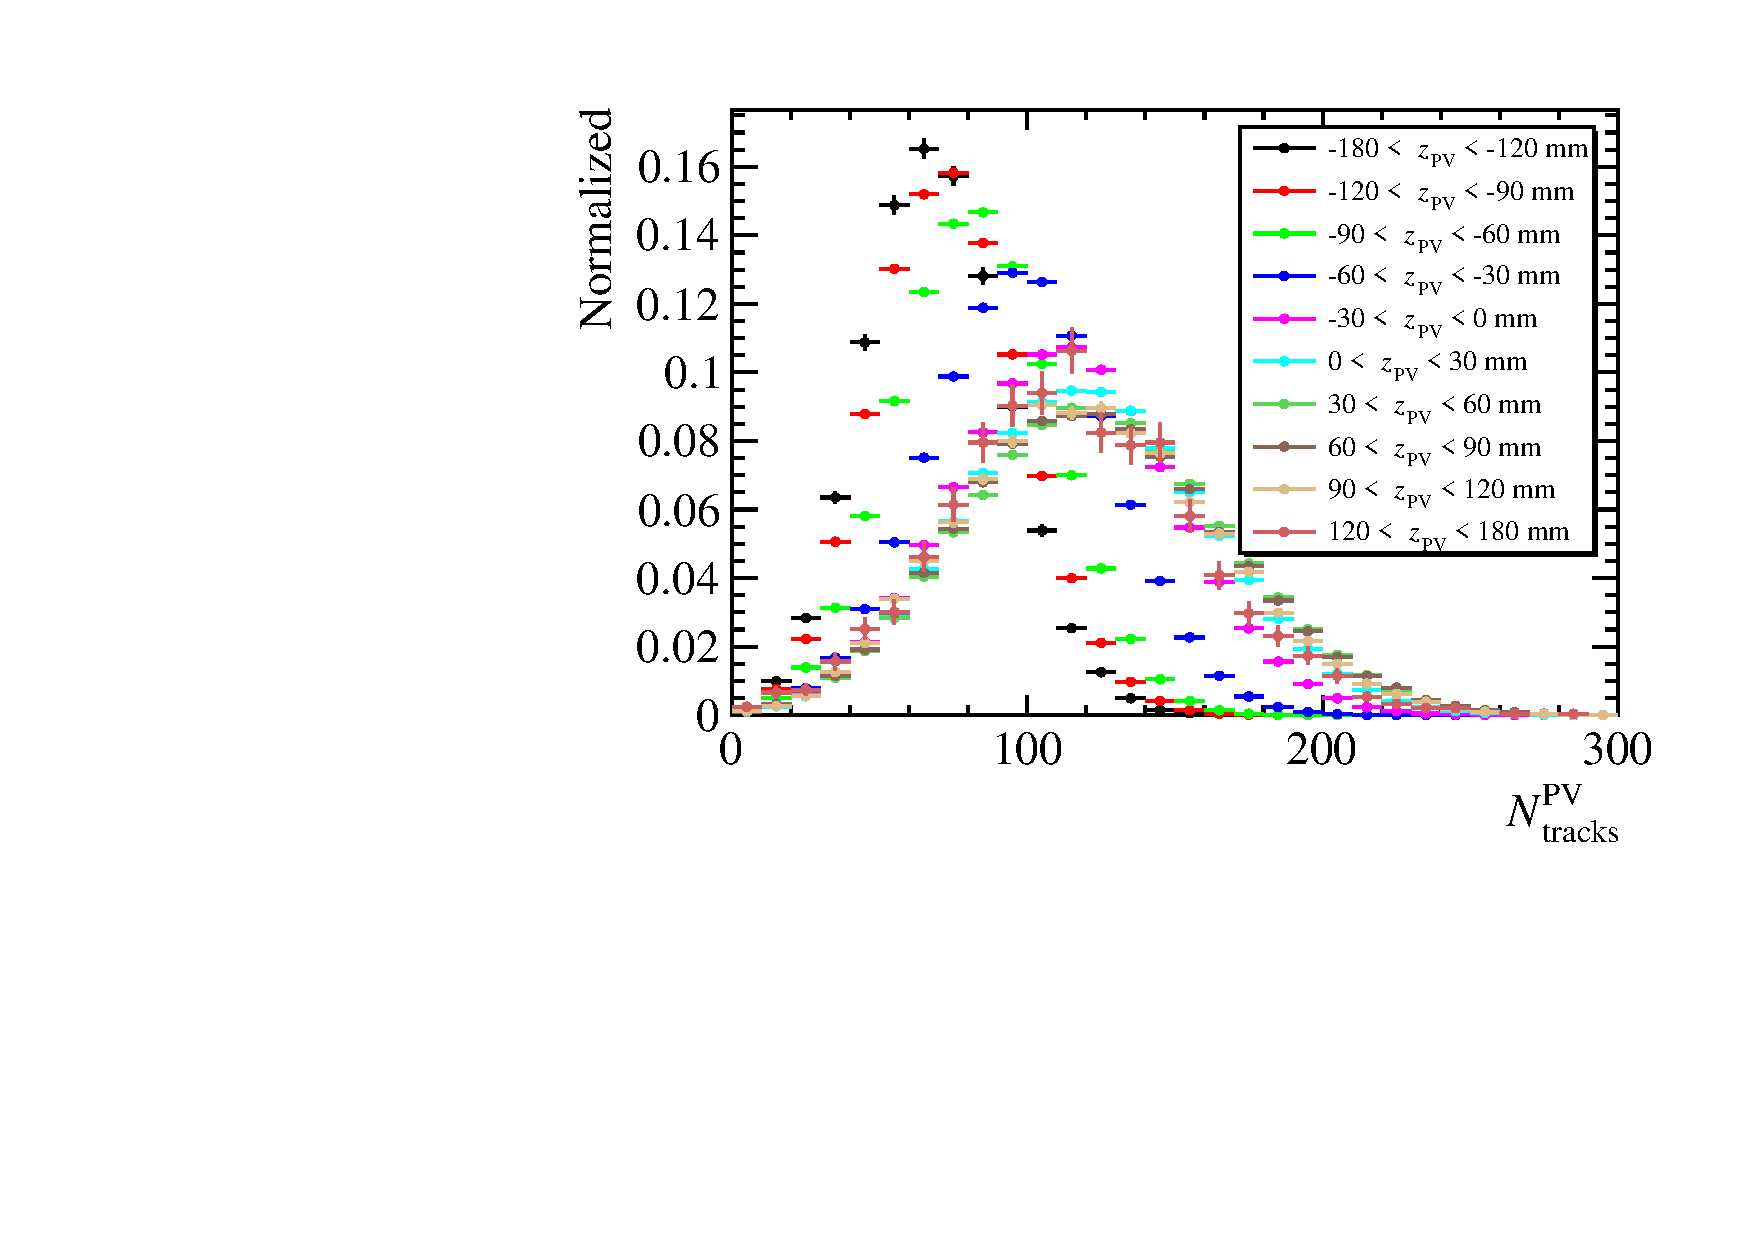
\includegraphics[width=0.49\linewidth]{pdf/pPb/Workdir/PVZvsMul/Jpsi.pdf}
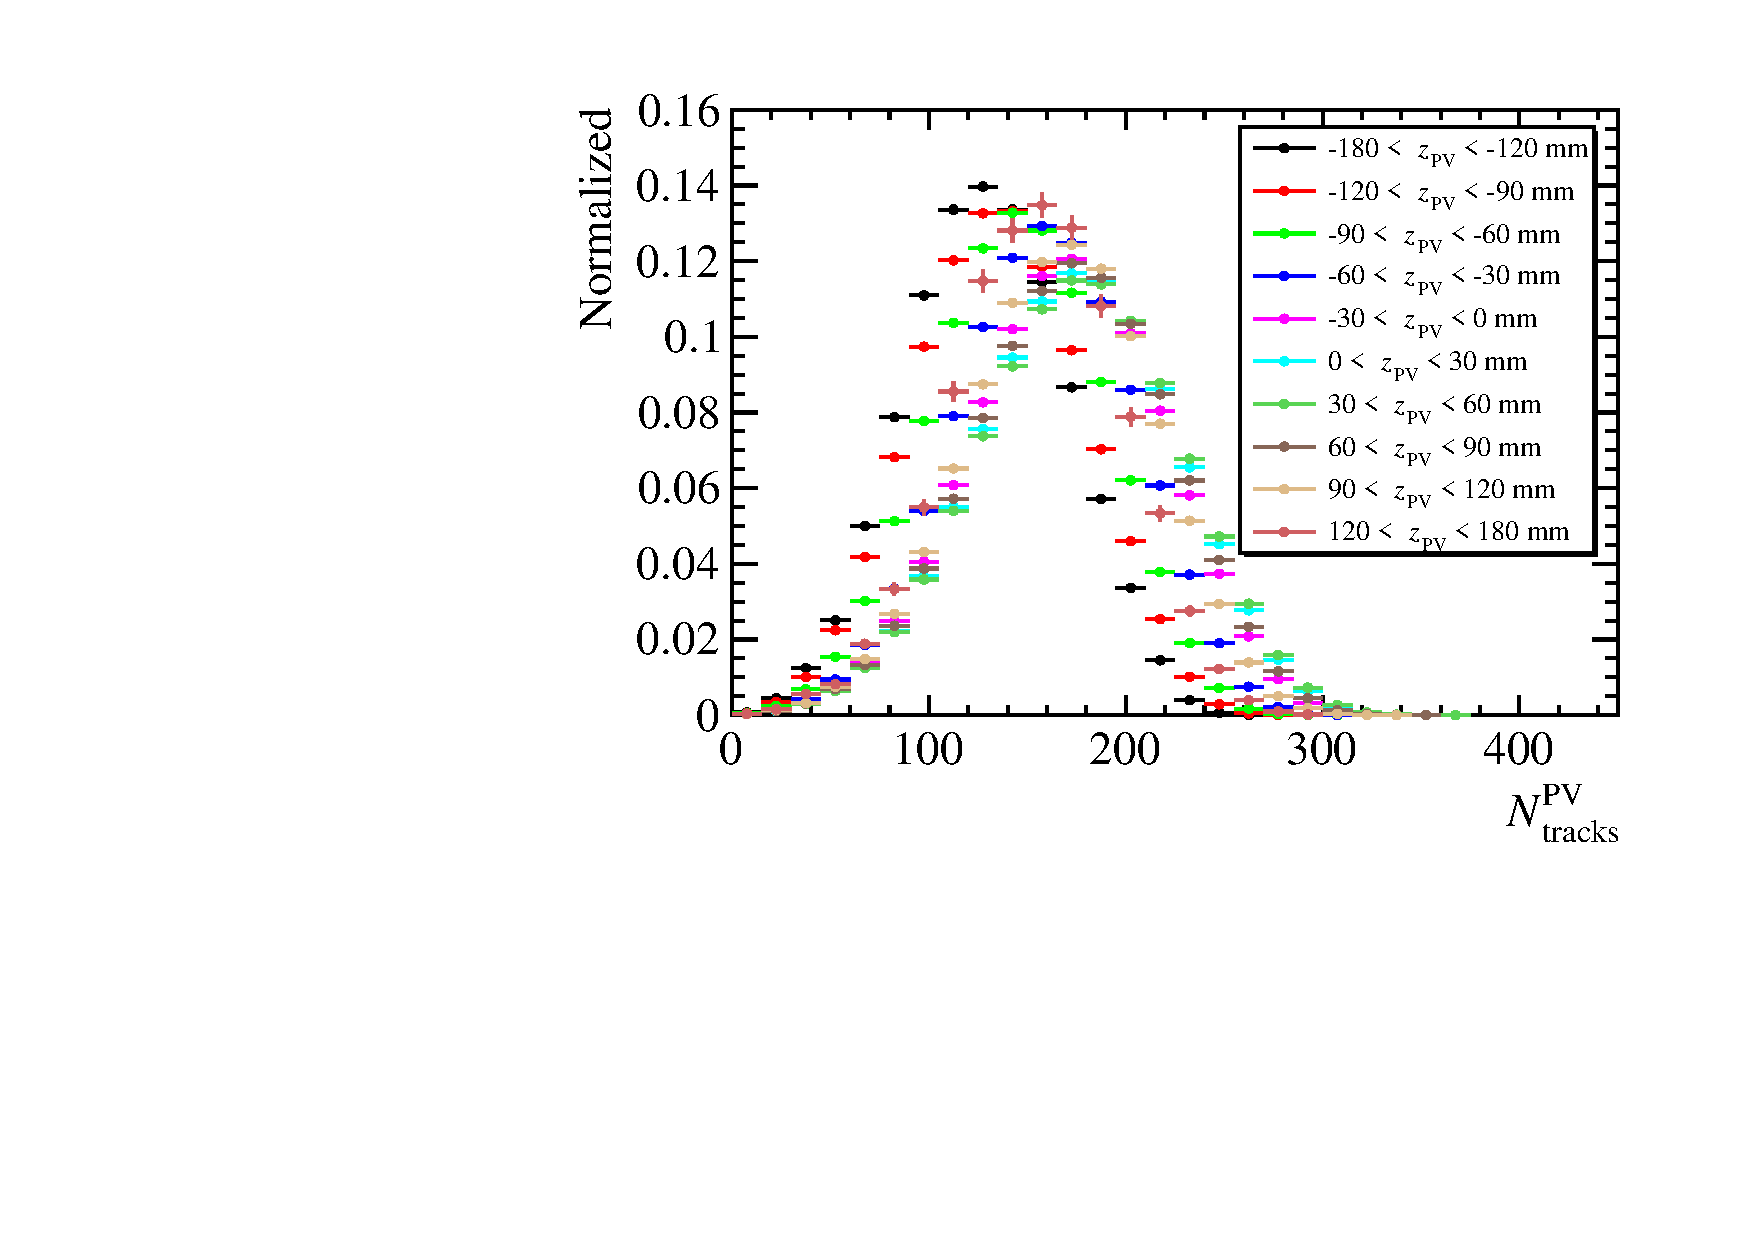
\includegraphics[width=0.49\linewidth]{pdf/Pbp/Workdir/PVZvsMul/Jpsi.pdf}
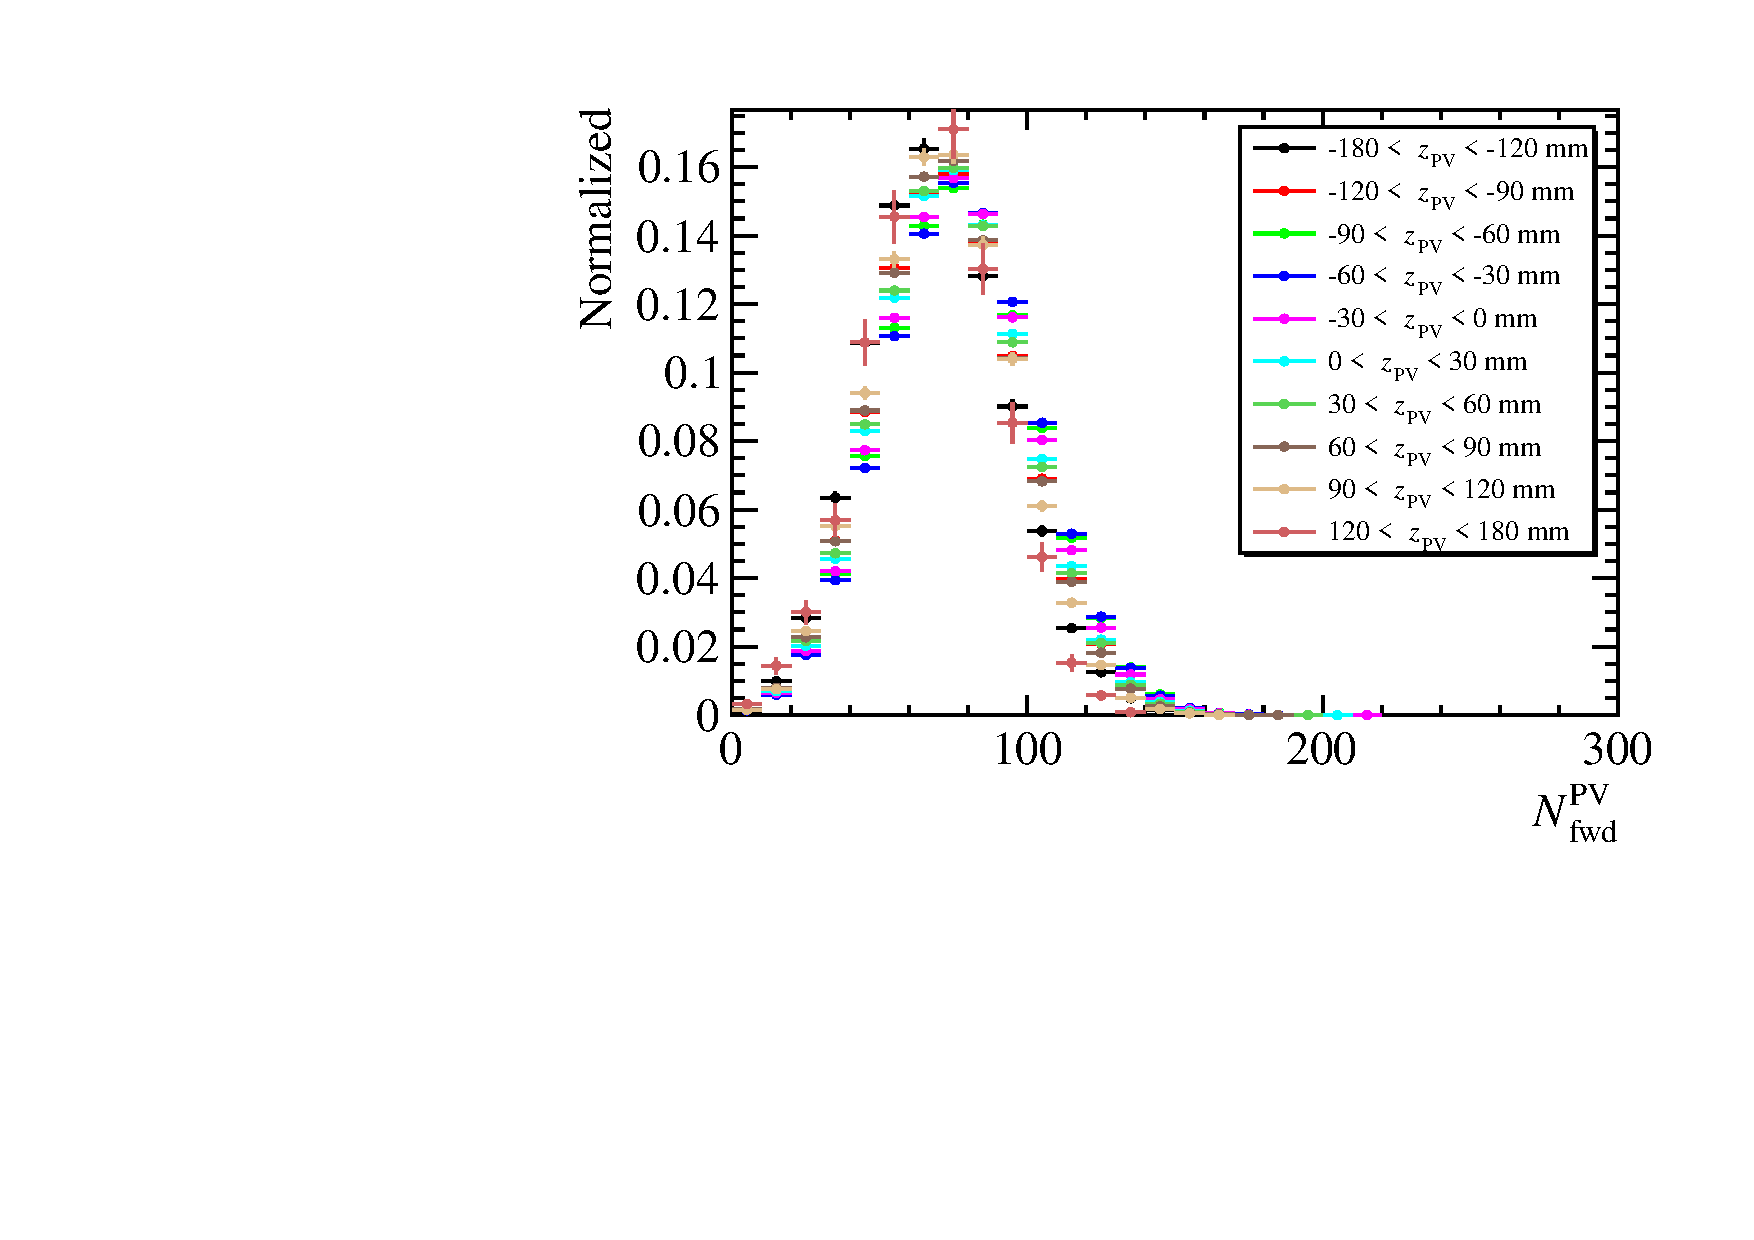
\includegraphics[width=0.49\linewidth]{pdf/pPb/FWorkdir/PVZvsMul/Jpsi.pdf}
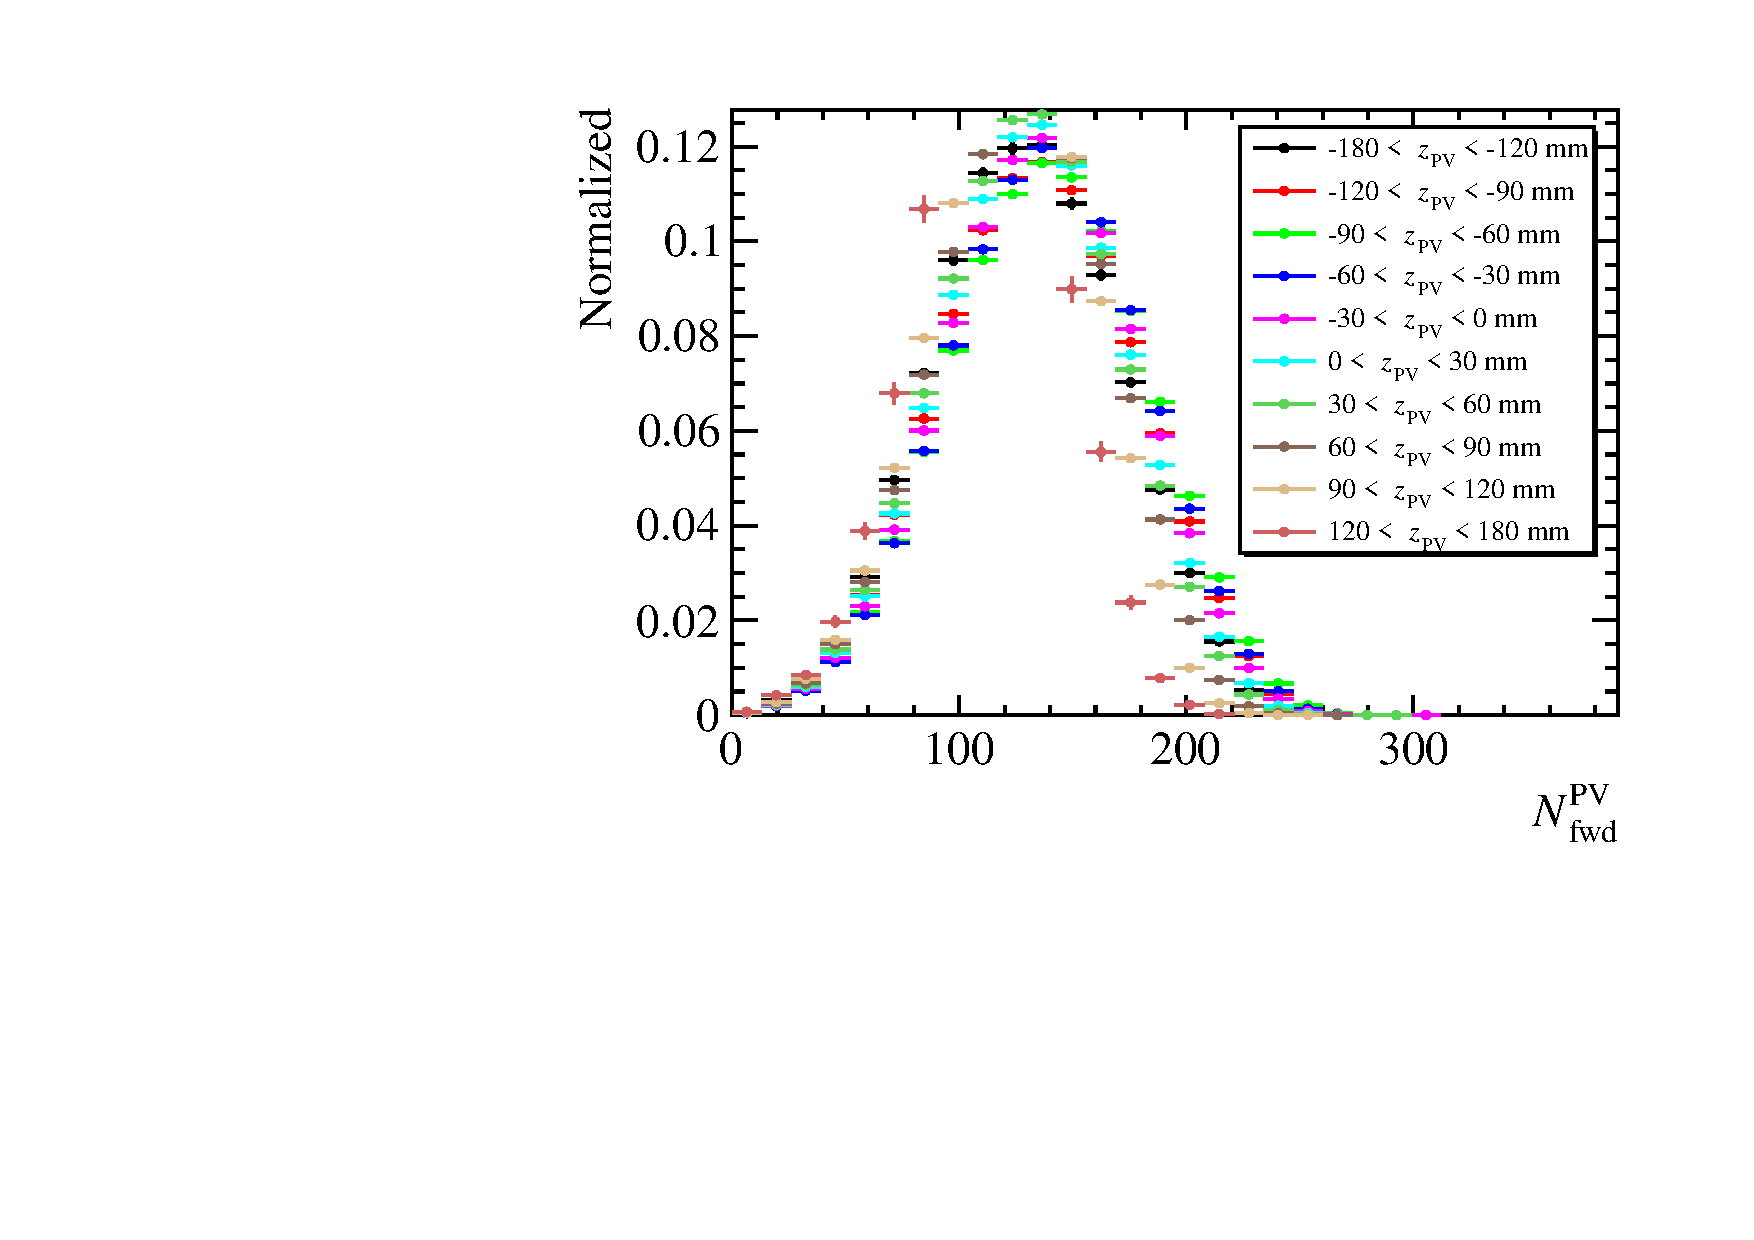
\includegraphics[width=0.49\linewidth]{pdf/Pbp/FWorkdir/PVZvsMul/Jpsi.pdf}
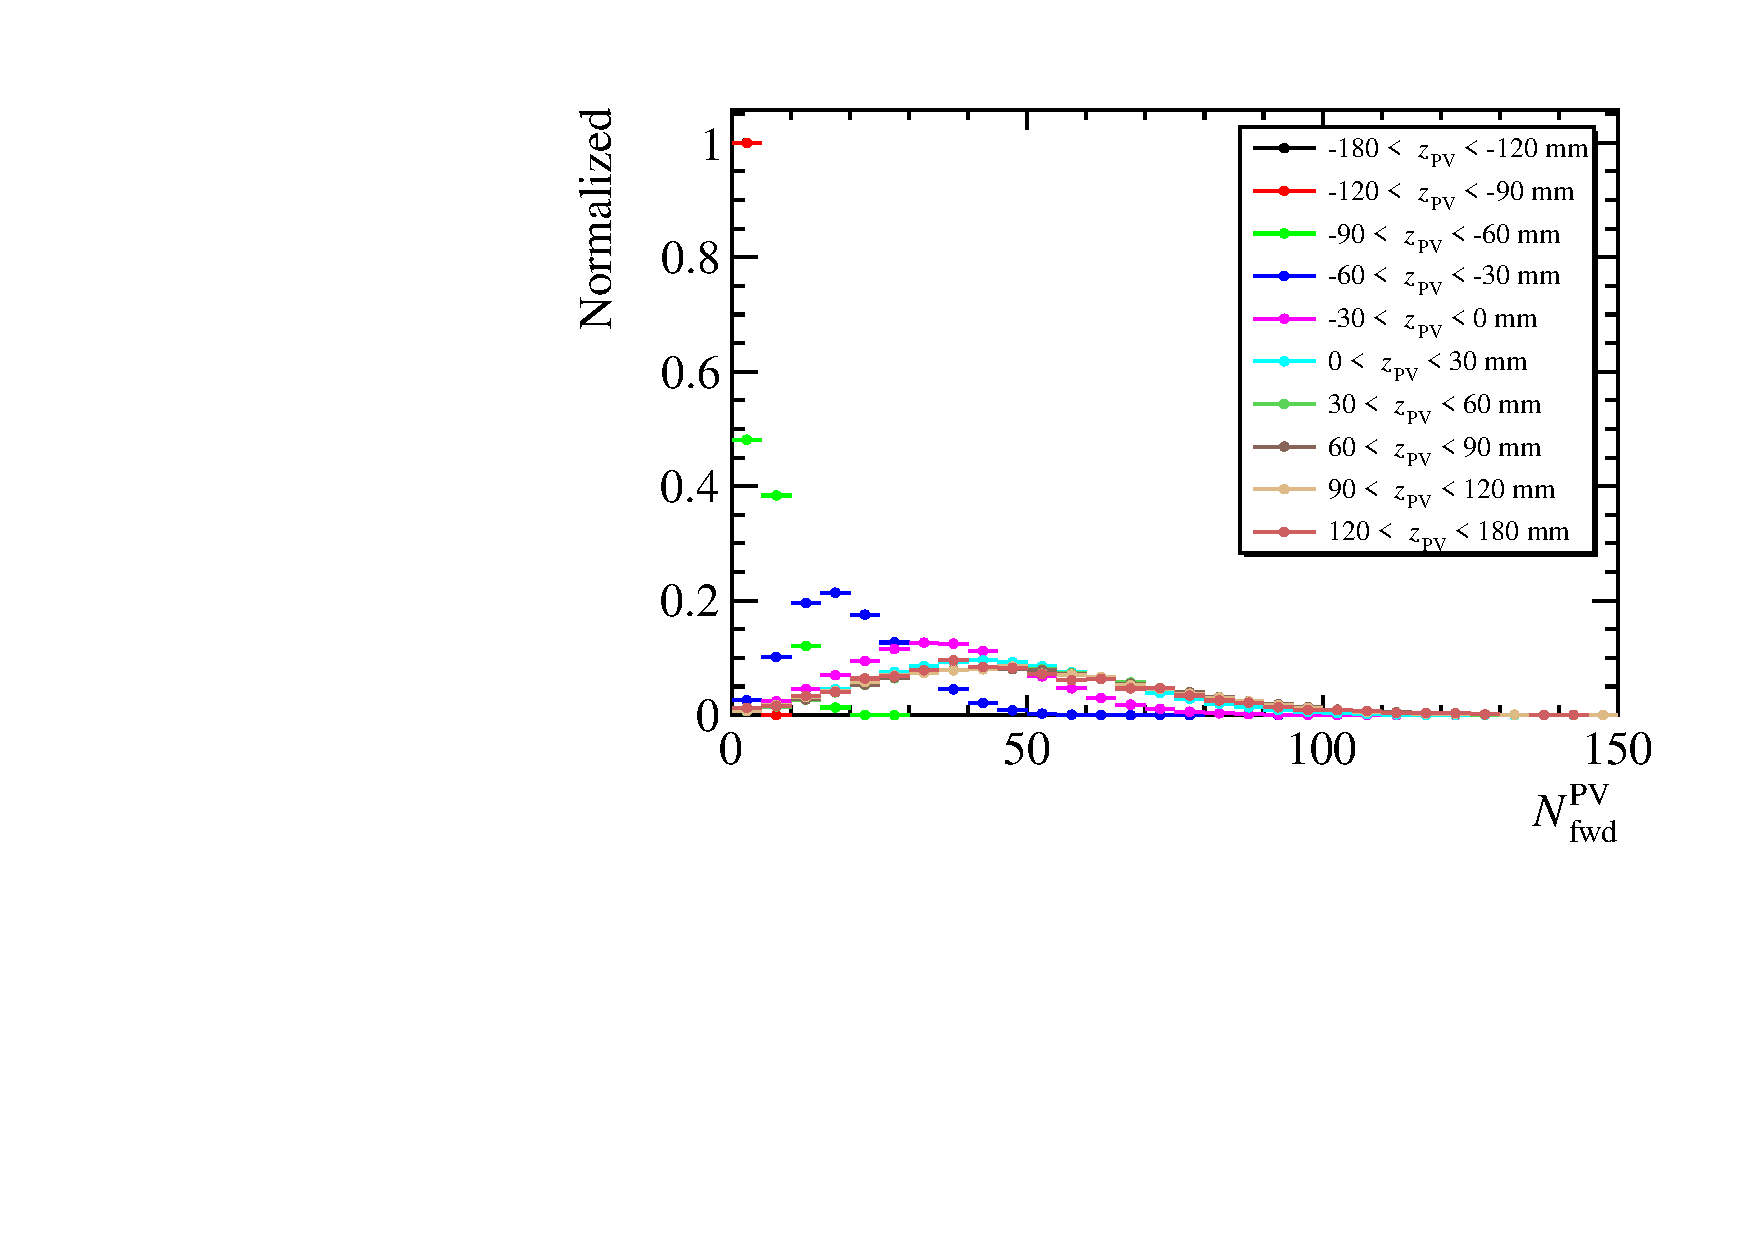
\includegraphics[width=0.49\linewidth]{pdf/pPb/BWorkdir/PVZvsMul/Jpsi.pdf}
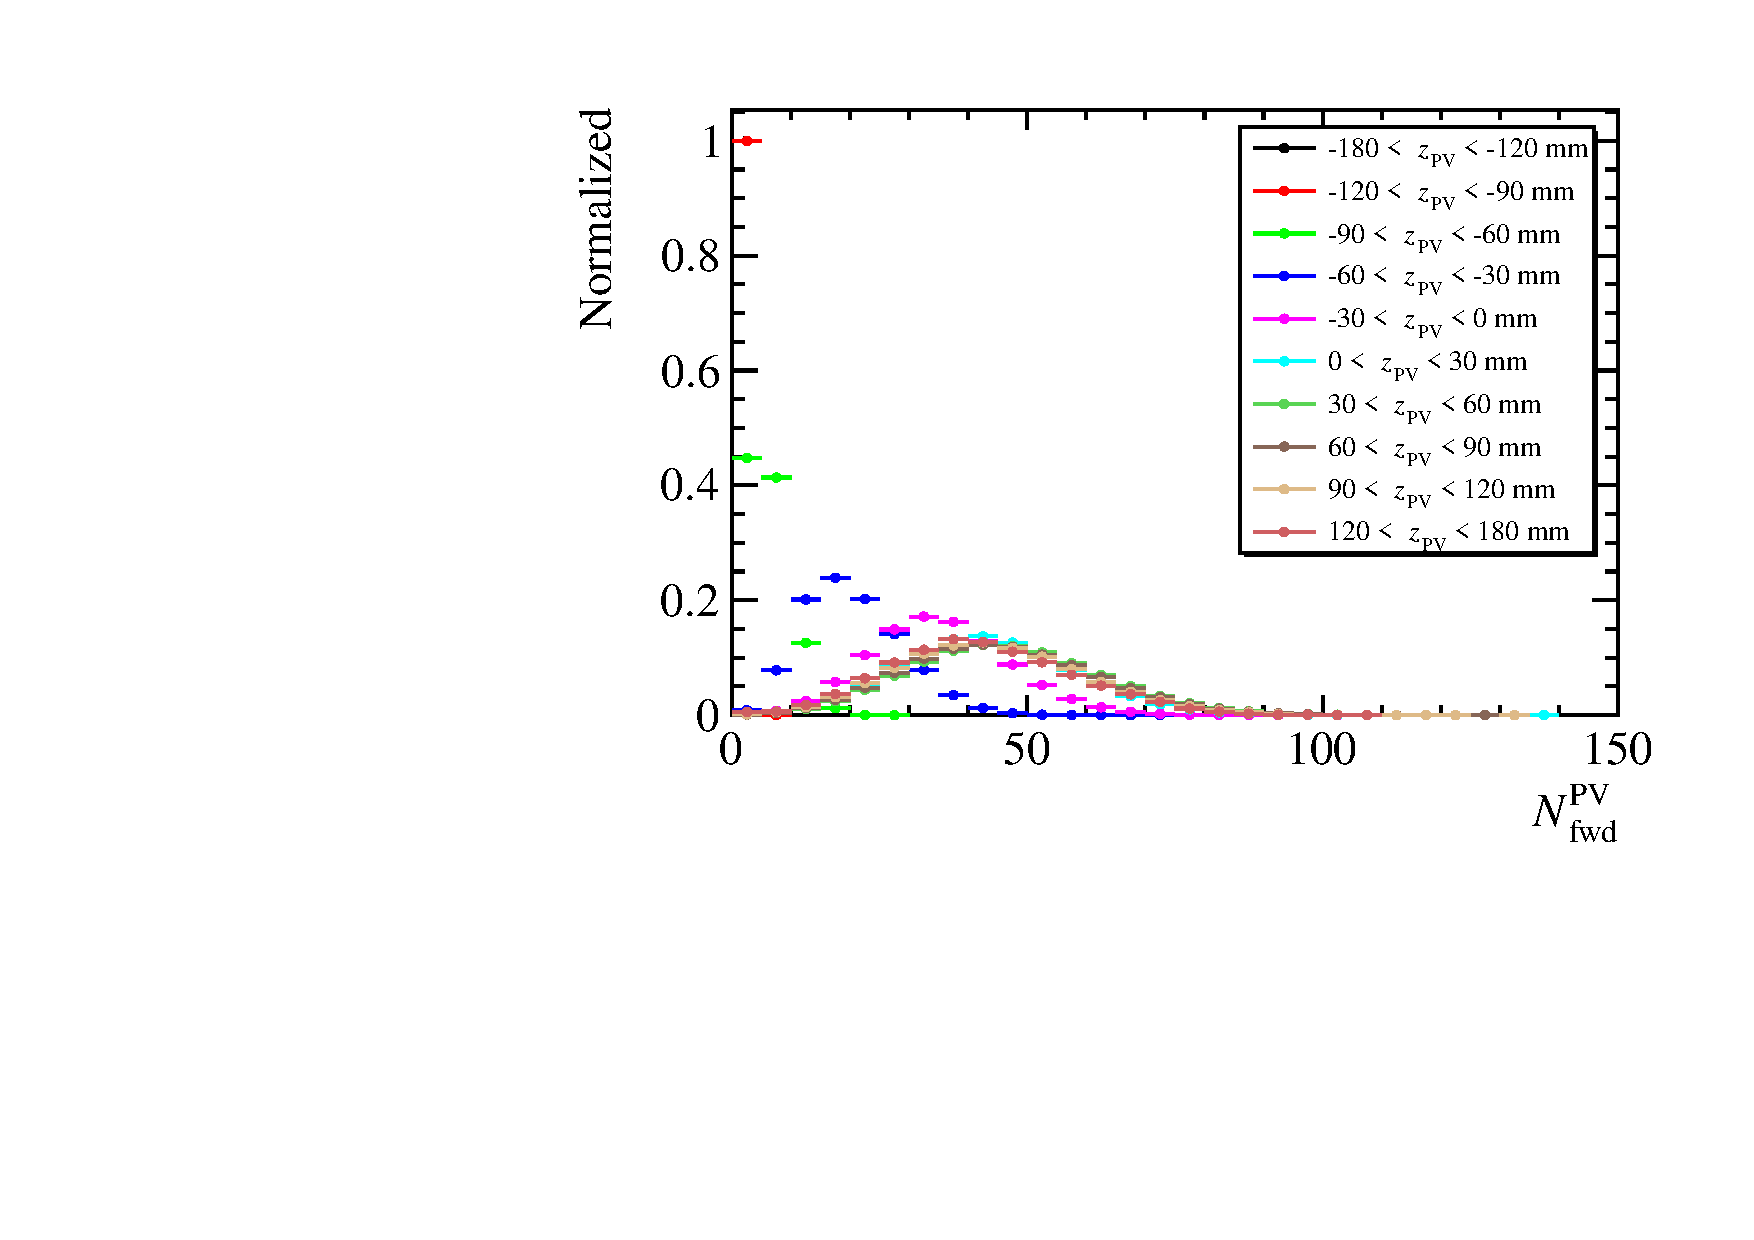
\includegraphics[width=0.49\linewidth]{pdf/Pbp/BWorkdir/PVZvsMul/Jpsi.pdf}
\end{center}
\caption{
    Distribution of (top) $N_{\rm tracks}^{\rm PV}$, (middle)  $N_{\rm fwd}^{\rm PV}$, (bottom) $N_{\rm bwd}^{\rm PV}$ in different $z_{\rm PV}$ ranges for \jpsi in (left) $p$Pb collisions and (right) Pb$p$ collisions.}
\label{JpsiPVZ}
\end{figure}

\subsection{Candidate Selection}
The \jpsi and \psitwos candidates are formed from two oppositely charged muons coming from a common vertex. Both decay modes are using same selection criteria. They are required to be TOS (Trigger On Signal) for the L0Muon and Hlt1DiMuonHighMass trigger lines, i.e. that the reconstructed candidate or its decay products are associated with a trigger object fulfilling the trigger requirements. Then the candidates used are directly the ones selected by the line Hlt2DiMuonJPsiTurbo and Hlt2DiMuonPsi2STurbo lines respectively, in the TURBO stream, without offline reconstruction. 
Additional cuts are applied at the analysis level. Muon tracks have to be in the geometrical acceptance of the spectrometer ($2 < \eta < 5$) and to have \pt $>$ 900 \mevc in order to improve the signal over background ratio. Both tracks are required to have a good fit quality, $\chi^2/ndof < 3$ and a ghost probability less than 0.4. They are identified as muons by requiring ProbNN($\mu$) $>$ 0.9 for both \jpsi and \psitwos. This is a harsh but appropriate PID cut since it can significantly reduce the background of high-multiplicity \psitwos data sample. And for low-multiplicity region, it doesn't remove too much of the signals. We can therefore achieve relative low statistical uncertainties when fitting the invariant mass spectrum and pseudo decay time spectrum, since the dominant uncertainties are statistical uncertainties of \psitwos which will be discussed later. The comparison for high- and low-multiplicity region of loose PID cut (ProbNN($\mu$) $>$ 0.6) and tight PID cut (ProbNN($\mu$) $>$ 0.9) can be seen in Figure~\ref{ProbNNmu}.
In addition, for both \jpsi and \psitwos, the two muons are required to form a good vertex asking the vertex fit probability Prob($\chi^2$) $>$ $0.5\%$. The \psitwos and \jpsi candidates are required to have a mass within 120 \mevcc of the PDG value. All selection criteria are specified in Table~\ref{OfflineSelection}.
\begin{table}[H]
\caption{Offline selection for \jpsi and \psitwos.}
\begin{center}
\begin{tabular}{ll}
\hline
\textbf{Variable} & \textbf{Cuts}\\
\hline
	$\mu^{\pm} \eta$ & $2<\eta<5$\\
	$\mu^{\pm} \pt$ & $>$900 \mevc\\
	ProbNNmu & $>$0.9\\
	TrackGhost Prob. & $<$0.4\\
	Vertex $\chi^2$ Prob. & $>0.5\%$\\
	Track $\chi^2/ndof$ & $<$3\\
	mass window & $\pm$ 120 \mevcc\\
\hline
\end{tabular}
\end{center}
\label{OfflineSelection}
\end{table}
\begin{figure}[!tbp]
\begin{center}
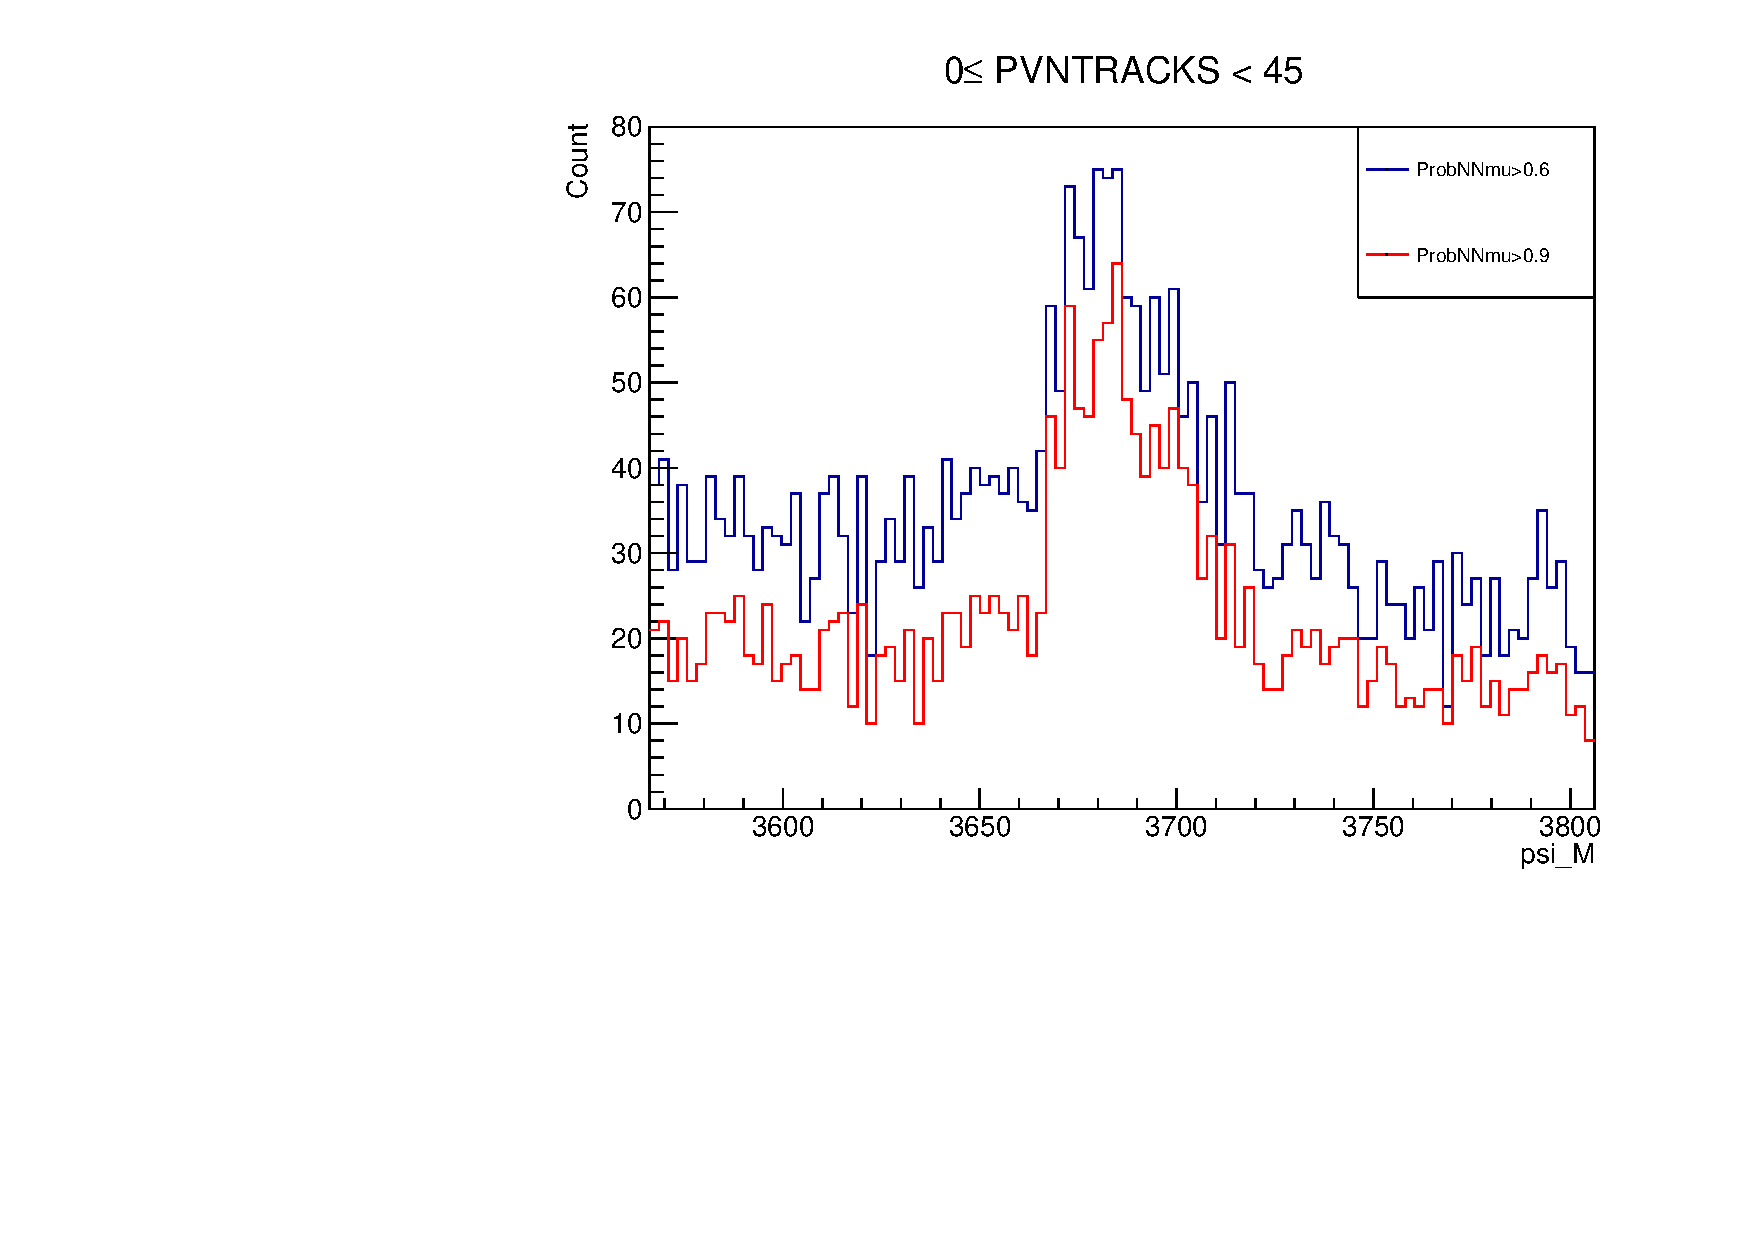
\includegraphics[width=0.7\linewidth]{pdf/pPb/Workdir/Psi_M_ProbNNmu/Low.pdf}
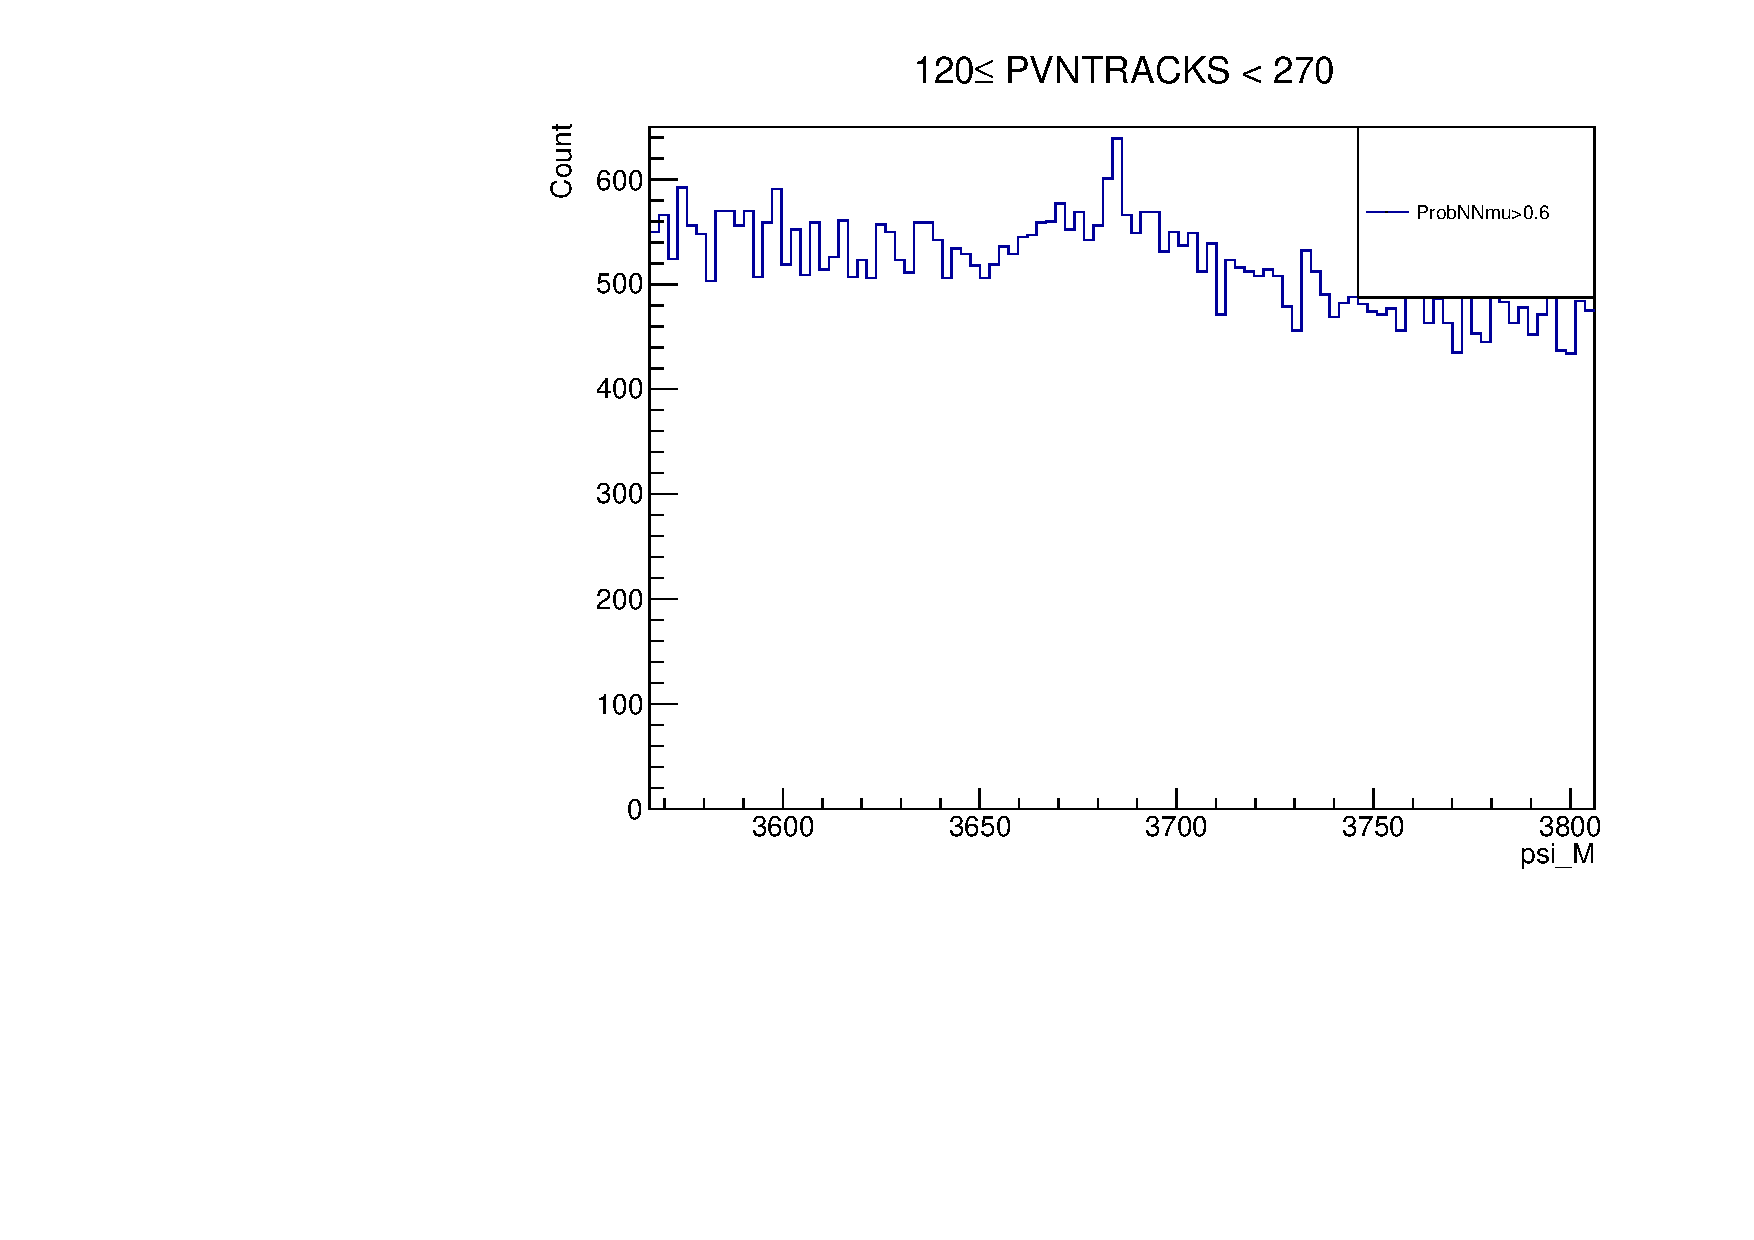
\includegraphics[width=0.49\linewidth]{pdf/pPb/Workdir/Psi_M_ProbNNmu/High1.pdf}
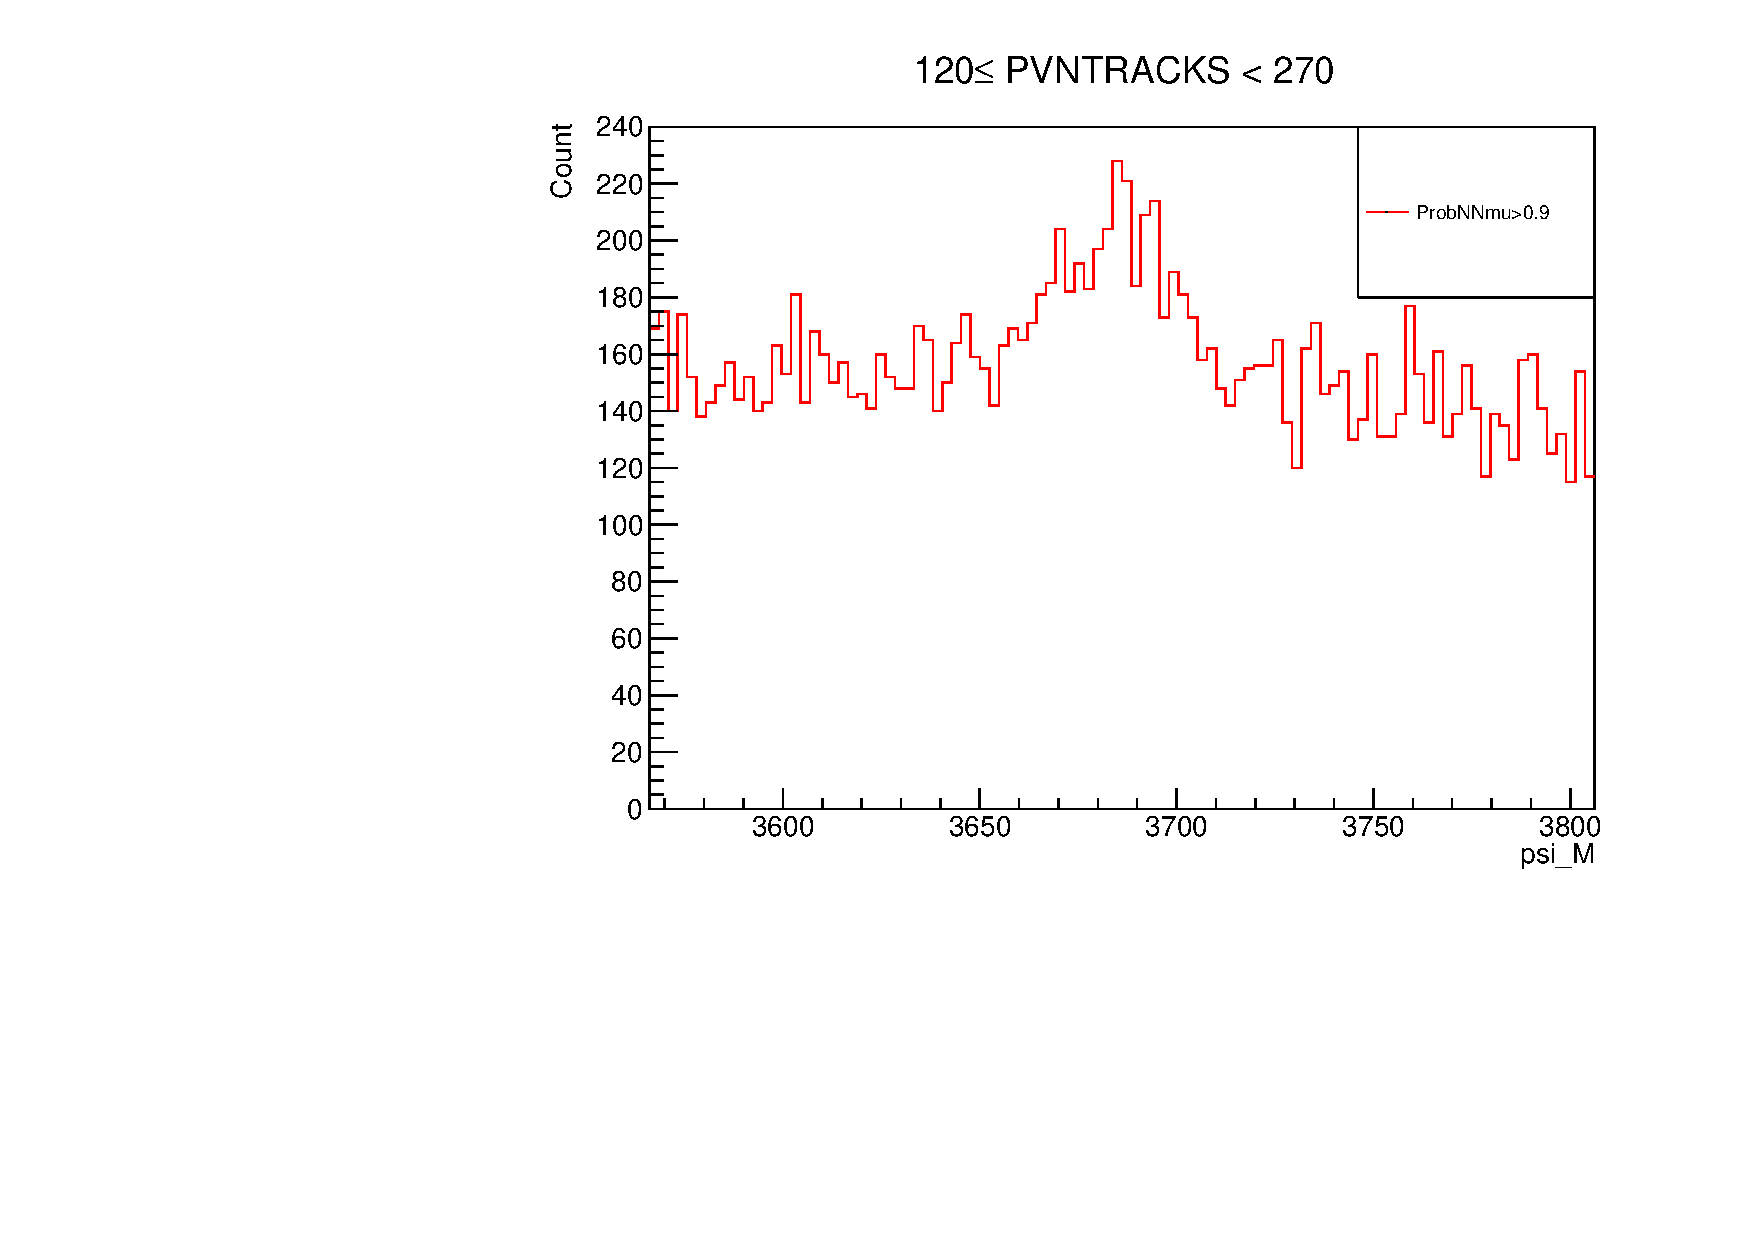
\includegraphics[width=0.49\linewidth]{pdf/pPb/Workdir/Psi_M_ProbNNmu/High2.pdf}
\end{center}
\caption{
	Mass spectrum of \psitwos after online and offline cuts with loose PID cut (blue) and tight PID cut (red). The first row is for lowest-multiplicity class and the second row is for highest-multiplicity class.}
\label{ProbNNmu}
\end{figure}


%%%%%%%%%%%%%%%%%%%%%%%%%%%%%%%%%%%%%%%%%%%%%%%%%%%%%%%%%%%%%%%%%%Multiplicity Variable%%%%%%%%%%%%%%%%%%%%%%%%%%%%%%%%%%%%%%%%%%%%%%%%%%%%%%%%%%%%%%%%%%%%%%%%%%%%%%%%%%
\section{Definition of observables}
\label{Observables}
\def\effTot{\ensuremath{\epsilon_{\mathrm{tot}}}\xspace}
\def\effAcc{\ensuremath{\epsilon_{\mathrm{acc}}}\xspace}
\def\effReco{\ensuremath{\epsilon_{\mathrm{Reco\&Sel}}}\xspace}
\def\effID{\ensuremath{\epsilon_{\mathrm{MuonID}}}\xspace}
\def\effTrigger{\ensuremath{\epsilon_{\mathrm{Trigger}}}\xspace}
All observables involved in this analysis are multiplicity variables, cross-sections and ratios of cross-sections. For cross-sections and the ratios, they require efficiency corrections to event yields obtained from data. The raw event yields are extracted from a combined fit of the di-muon invariant mass and of the pseudo-proper decay time to separate the prompt and the from-$b$ signal contributions, where the pseudo-proper decay time is defined in Eq.~\ref{tz}.
\begin{equation}
	t_z=\frac{(z_{\jpsi(\psitwos)}-z_{PV})\times M_{\jpsi(\psitwos)}}{p_z},   
\label{tz}
\end{equation}
with $z_{\jpsi(\psitwos)}$ the z-coordinate of the \jpsi or \psitwos decay vertex and $z_{\rm PV}$ the z-coordinate of the primary vertex.
\textbf{Prompt} here means produced directly at the nucleon-nucleon interaction, or via a decay of a charmonium produced directly at the interaction (such as a $\chi_c\rightarrow \jpsi \gamma$ decay). \textbf{from-$b$} means a charmonium coming from a $B$ decay (either directly, or via a charmonium decay where the higher charmonium state is produced in a $B$ decay). The observables of the analysis are measured separately for the prompt and from-$b$ production components. Given the large statistics available, the observables are also computed in bin of \pt, the transverse momentum with respect to the beam axis and of $y^*$, the rapidity with respect to the beam axis in the center-of-mass frame, taking the direction of the proton beam to define the polar axis, and neglecting the small angle between the two due to the crossing angle of the two beams at LHCb. The rapidity is related to the rapidity in the lab frame, $y_{lab}$, with $y^* = y_{lab} - 0.465$ for the $p$Pb configuration and with $y^* = -(y_{lab} + 0.465)$ for the Pb$p$ configuration. For $pp$ collisions (used as reference in the various ratios given below), $y^*=y_{lab}$.

\subsection{Multiplicity variables}
For $p$Pb and Pb$p$ configurations, the variables we used to separate multiplicity classes are $N_{\rm tracks}^{\rm PV}$, $N_{\rm bwd}^{\rm PV}$ and $N_{\rm fwd}^{\rm PV}$. Cross-sections and cross-section ratios are calculated in each multiplicity class and then we can get the cross-section ratios as a function of different multiplicity variables. For the \jpsi and \psitwos mesons, cross-sections are extracted in the rapidity range $1.5 < y^* < 4.0 (-5.0 < y^* < -2.5)$ for $p$Pb (Pb$p$), together with the transverse momentum range $0 < \pt < 14\gevc$. In this analysis, we do not separate any rapidity bin or transverse momentum bin due to poor statistics of \psitwos meson. And the systematic uncertainties due to that is discussed thoroughly in chapter for systematic uncertainties. After calculating the ratio of \psitwos-to-\jpsi cross-section ratios in each multiplicity bin, we will further normalized the multiplicity variables by dividing it by the mean values from \textbf{NoBias} data samples.
The binning schemes and mean values from \textbf{NoBias} data samples for different multiplicity variables are summarized in Table~\ref{MultiplicityBin}. This binning schemes are chosen to assure that in each multiplicity bin, there are enough \psitwos signal candidates that can be used in signal extraction. $N_{\rm tracks}^{\rm PV}$ starts at 4 since at least four tracks are required to form a primary vertex. 
\begin{table}[H]
\caption{Binning schemes for different multiplicity variables.}
\begin{center}
\begin{tabular}{c|c|l|c}
\hline
\textbf{Configurations} & \textbf{Mult. Variables} & \textbf{Schemes} & \textbf{Mean (NoBias)}\\
\hline
$p$Pb & $N_{\rm tracks}^{\rm PV}$ & 4, 45, 70, 90, 120, 270 & 60.54\\
\hline
$p$Pb & $N_{\rm fwd}^{\rm PV}$ & 0, 25, 43, 57, 72, 150 & 33.17 \\
\hline
$p$Pb & $N_{\rm bwd}^{\rm PV}$ & 0, 17, 29, 40, 54, 140 & 27.37 \\
\hline
Pb$p$ & $N_{\rm tracks}^{\rm PV}$ & 4, 60, 90, 120, 160, 330 & 69.54\\
\hline
Pb$p$ & $N_{\rm fwd}^{\rm PV}$ & 0, 35, 65, 85, 110, 250 & 47.07\\
\hline
Pb$p$ & $N_{\rm bwd}^{\rm PV}$ & 0, 13, 22, 30, 47, 120 & 22.47\\
\hline
\end{tabular}
\end{center}
\label{MultiplicityBin}
\end{table}

\subsection{Cross-sections and cross-section ratios}
 The absolute double differential cross-sections for \jpsi or \psitwos production are defined in Eq~\ref{CrossSec}.
\begin{equation}
    \frac{\deriv^2\sigma}{\deriv y^*\deriv \pt}\bigg|_{Mult. \ bin}
    = \frac{N}
           {\mathcal{L}\times\effTot\times \BR_{\mu\mu}\times\Delta y^* \times \Delta \pt}\bigg|_{Mult. \ bin}.
  \label{CrossSec}
\end{equation}
where N represents the raw yield of the \jpsi or \psitwos reconstructed in the given multiplicity bin within the rapidity and transverse momentum ranges mentioned above, \effTot the total efficiency, including acceptance, $\BR_{\mu\mu}$ the branching ratio of the \jpsi or \psitwos decay in two muons and $\mathcal{L}$ the integrated luminosity of the given data sample. The values of branching ratio $\BR(\jpsi\rightarrow\mu^+\mu^-)=(5.961\pm0.033)\%$ is the branching fraction of the decay $\jpsi\rightarrow \mu^+ \mu^-$, and $\BR(\psitwos\rightarrow e^+e^-)=(7.93\pm0.17)\times10^{-3}$ is the branching fraction of the decay $\psitwos\rightarrow e^+ e^-$, quoted from the PDG 2022 review~\cite{Workman:2022ynf}. The dielectron branching fraction is used for \psitwos since it has a much smaller uncertainty than the dimuon one. Assuming lepton universality, the $\BR(\psitwos\rightarrow e^+e^-)$ is used to compute the cross-section.
Cross-section ratio is defined in Eq.~\ref{CS_ratio}. The width of rapidity, transverse momentum and integrated luminosity are canceled out.
\begin{equation}
    \frac{\deriv^2\sigma_{\psitwos}/\deriv y^*\deriv \pt}{\deriv^2\sigma_{\jpsi}/\deriv y^*\deriv \pt}\bigg|_{Mult. \ bin}
    =\frac{\BR(\jpsi \rightarrow \mu^+ \mu^-)}{\BR(\psitwos\rightarrow e^+e^-)}\times \frac{N_{\psitwos}}{N_{\jpsi}}\bigg|_{Mult. \ bin}\times \frac{\ensuremath{\epsilon_{\mathrm{tot,\jpsi}}}}{\ensuremath{\epsilon_{\mathrm{tot,\psitwos}}}}\bigg|_{Mult. \ bin}.
\label{CS_ratio}
\end{equation}


%%%%%%%%%%%%%%%%%%%%%%%%%%%%%%%%%%%%%%%%%%%%%%%%%%%%%%%%%%%%%%%%%%%%%Signal Extraction%%%%%%%%%%%%%%%%%%%%%%%%%%%%%%%%%%%%%%%%%%%%%%%%%%%%%%%%%%%%%%%%%%%%%%%%%%%%%%%%%%%
\section{Signal extraction}
\label{Signal extraction}
The numbers of prompt and from-$b$ \jpsi and \psitwos signal candidates are extracted from a simultaneous fit to the invariant mass and pseudo-proper time $t_z$ distributions. For prompt production, $t_z$ is equal to 0 while for charmonium coming from the decay of a $B$ hadron, $t_z$ is a good approximation of the $B$ hadron propertime and should follow an exponential distribution.

\subsection{Mass fit function}
The procedure that is described in the following is very close to the one used in previous $pp$ analyses~\cite{LHCb:2015foc}. The function describing the invariant mass of the signal candidates is a Crystal Ball function defined in Eq.~\ref{CBfunction}.
\begin{equation}
 f_{\mathrm{CB}}(m;\mu,\sigma,\alpha,n) =
 \begin{cases}
      \Big(\frac{n}{|\alpha|}\Big)^n e^{-\frac{1}{2}\alpha^2} (\frac{n}{|\alpha|}-|\alpha|-\frac{m-\mu}{\sigma})^{-n} & \frac{m-\mu}{\sigma} < -|\alpha|\\
   \exp\Bigg( -\frac{1}{2}\Big(\frac{m-\mu}{\sigma}\Big)^2\Bigg) & \frac{m-\mu}{\sigma}>-|\alpha|.
\end{cases}.
\label{CBfunction}
\end{equation}
The value of the parameter n is fixed to 1 following the physics arguments described in Ref.~\cite{LefrancoisTalk}, while the value of the parameter $\alpha$ is constrained from the values of the resolution parameter $\sigma$ following
\begin{equation}
\alpha = 2.066+0.0085\sigma-0.00011\sigma^2,
\label{alphasigma}
\end{equation}
 extracted from toy Monte Carlo studies and where $\sigma$ is expressed in \mev. The background, which is only combinatorial, is described by an exponential function,
\begin{equation}
f_{bkg}(x;p)=e^{-px}.
\end{equation}
For \jpsi mass fit, two crystal ball function with common mean value are applied to describe the signals while for \psitwos, only one is used.
\subsection{Pseudo-propertime fit function}
To determine the signal yields of prompt and from-\bquark components separately, the $t_z$ distribution is used. In each kinematic and multiplicity bin, an unbinned extended maximum likelihood fit to the two-dimensional distributions of invariant mass $m(\mumu)$ and $t_z$ is performed to separate prompt component from that from \bquark.
At the generator level, the $t_z$ distribution of the prompt component is a Dirac delta function, $\delta(t_z)$, while that from $\bquark$ follows an exponential function as seen from simulation. For \jpsi and \psitwos signals, the detector resolution is taken into account by convolving a resolution function, which is described by the sum of two Gaussian functions with a common mean and resolution parameters $\sigma$ and $2\sigma$ respectively:
\begin{equation}
f_\mathrm{resolution}(t_z;\mu,\sigma,\beta) = \frac{\beta}{\sqrt{2\pi}\sigma} e^{-\frac{(t_z-\mu)^2}{2\sigma^2}}
+\frac{1-\beta}{2\sqrt{2\pi}\sigma} e^{-\frac{(t_z-\mu)^2}{8\sigma^2}}.
\end{equation}
The background control sample consists of random combinations of muons from semi-leptonic $\bquark$ and $\cquark$ decays, which tend to produce positive $t_z$ values, as well as mis-reconstructed tracks from decays-in-flight of kaons and pions, which contribute both to positive and negative $t_z$ values. The $t_z$ distribution of the background is therefore modeled with an empirical function, composed of a Dirac delta function and five exponentials (three for positive $t_z$ and two for negative $t_z$, with one positive $t_z$ and one negative sharing the same slope parameter). This function is convolved with the sum of two Gaussian functions as a resolution function, which has different parameters as for signals. The fit function for $t_z$ background is as follows,
\begin{align}
f_\mathrm{background} &=
\left[(1-f_1-f_2-f_3-f_4)\delta(t_z)+\theta(t_z)(\frac{f_1}{\tau_1}e^{-t_z/\tau_1}+\frac{f_2}{\tau_2}e^{-t_z/\tau_2})\right.
\nonumber\\
&\left. +\theta(-t_z)\frac{f_3}{\tau_3}e^{t_z/\tau_3}+\frac{f_4}{2\tau_4}e^{-|t_z|/\tau_4}
\right]\ast \left(\frac{\beta'}{\sqrt{2\pi}S^{'}_1\sigma} e^{-\frac{(t_z-\mu)^2}{2S^{'2}_1\sigma^2}}
  +\frac{1-\beta'}{\sqrt{2\pi}S^{'}_2\sigma} e^{-\frac{(t_z-\mu)^2}{2S^{'2}_2\sigma^2}}\right).
\label{eq:TzBKG}
\end{align}
The shape of the background is chosen empirically based on the shape seen in the $t_z$ distribution of the \jpsi and \psitwos mass side-bands, which are at 50 \mevcc away from the mass values from the PDG.
The fit procedures are as follows,
\begin{itemize}
\item First step, the one-dimensional fit to the mass spectrum is performed to estimate the yield and the parameters of inclusive (sum of prompt and from-$b$) signal candidates, the background yield and of the exponent of the background function.
\item Second step, the mass sideband candidates ($|M-M^{PDG}|>50\mevcc$) are used to fit the $t_z$ distribution for the background. 
\item Last step, a simultaneous fit to the mass and the pseudo-proper decay time distributions is then performed.
\end{itemize}

As examples, the $t_z$ background fit for \jpsi and \psitwos are shown in Figure~\ref{fig_tzbkg} for $4\leq N_{\rm tracks}^{\rm PV} < 45$ in $p$Pb  configuration and the 2-dimensional fit projected in mass spectrum and $t_z$ spectrum are shown in Figure~\ref{fig_2DFit} for $4\leq N_{\rm tracks}^{\rm PV} < 45$ in  $p$Pb configuration. The fit results for other multiplicity class in $p$Pb and Pb$p$ configurations can be found in appendix.
\begin{figure}[!tbp]
\begin{center}
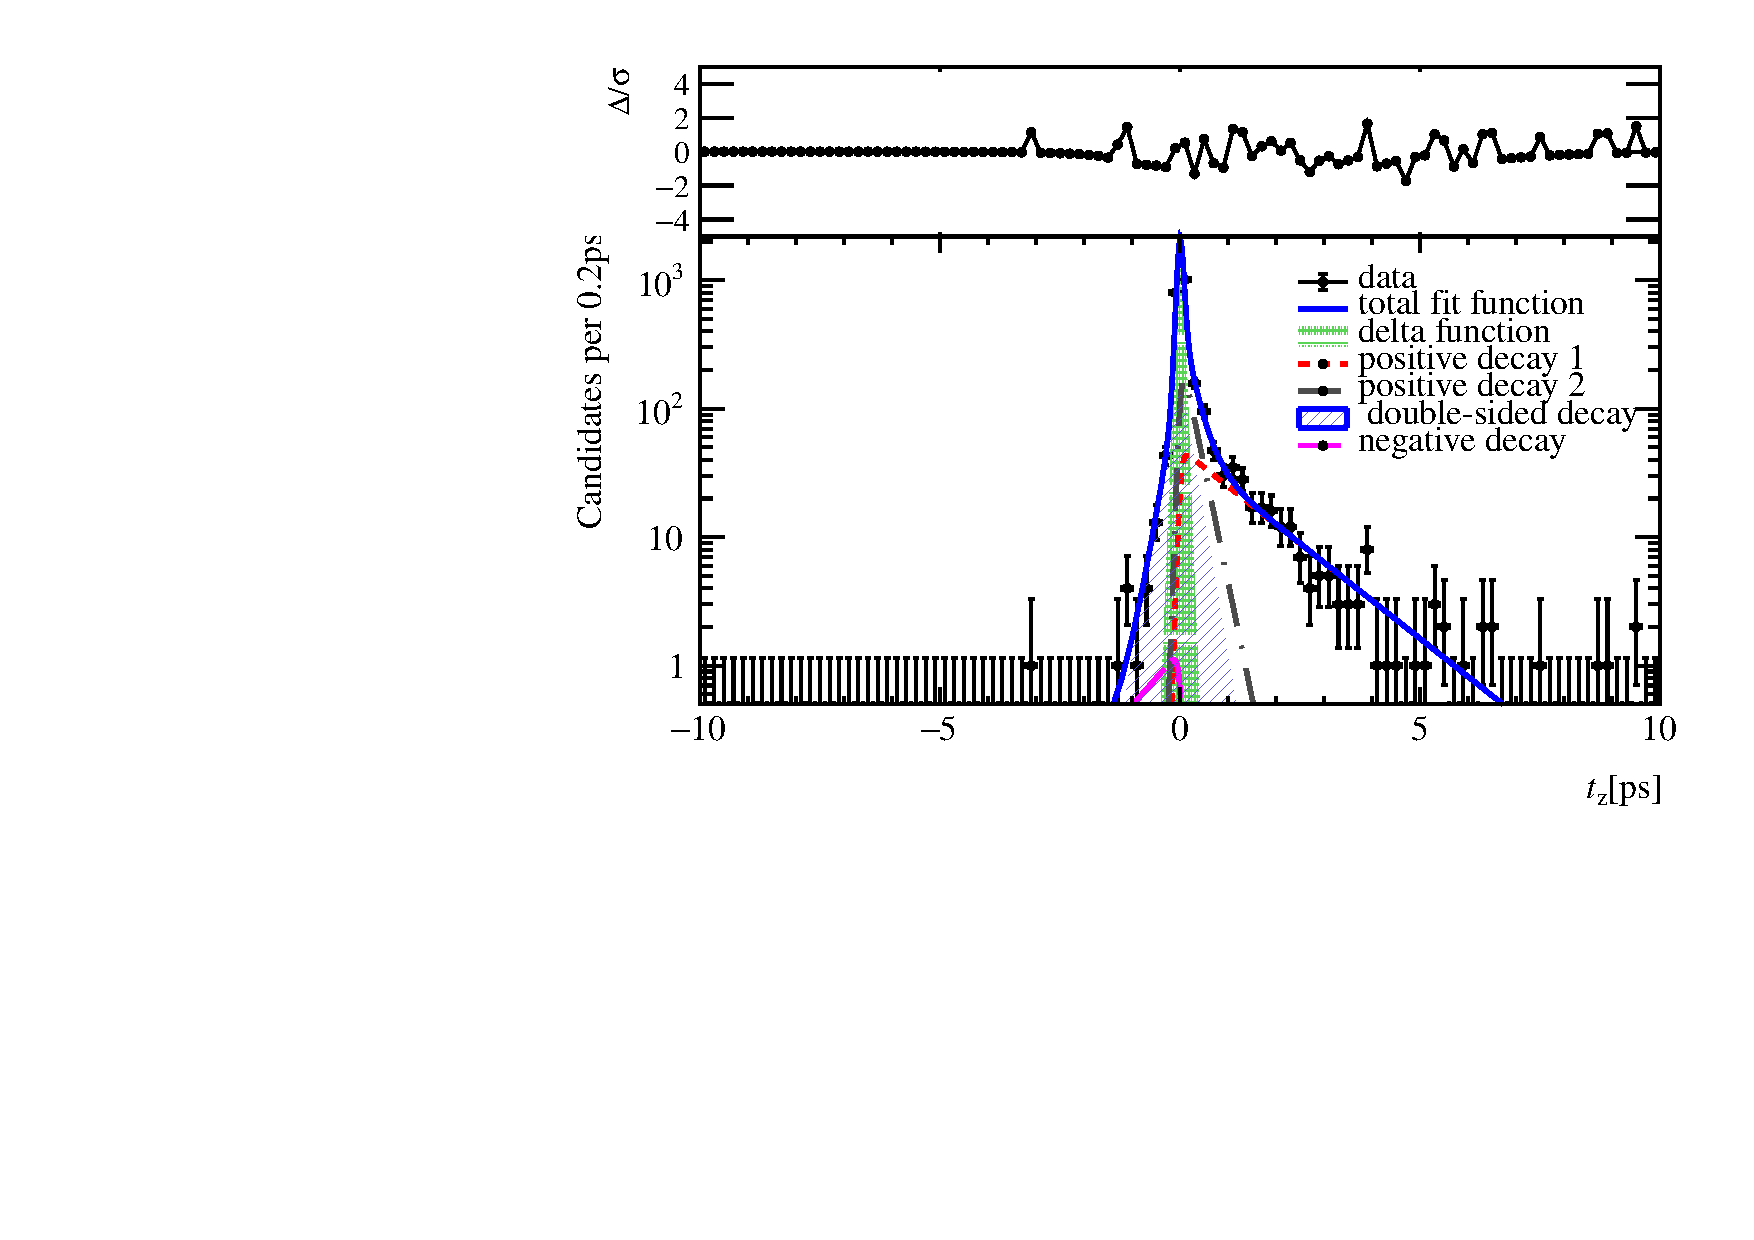
\includegraphics[width=0.49\linewidth]{pdf/pPb/Workdir/TzbkgFit/Jpsi_n1y1pt1.pdf}
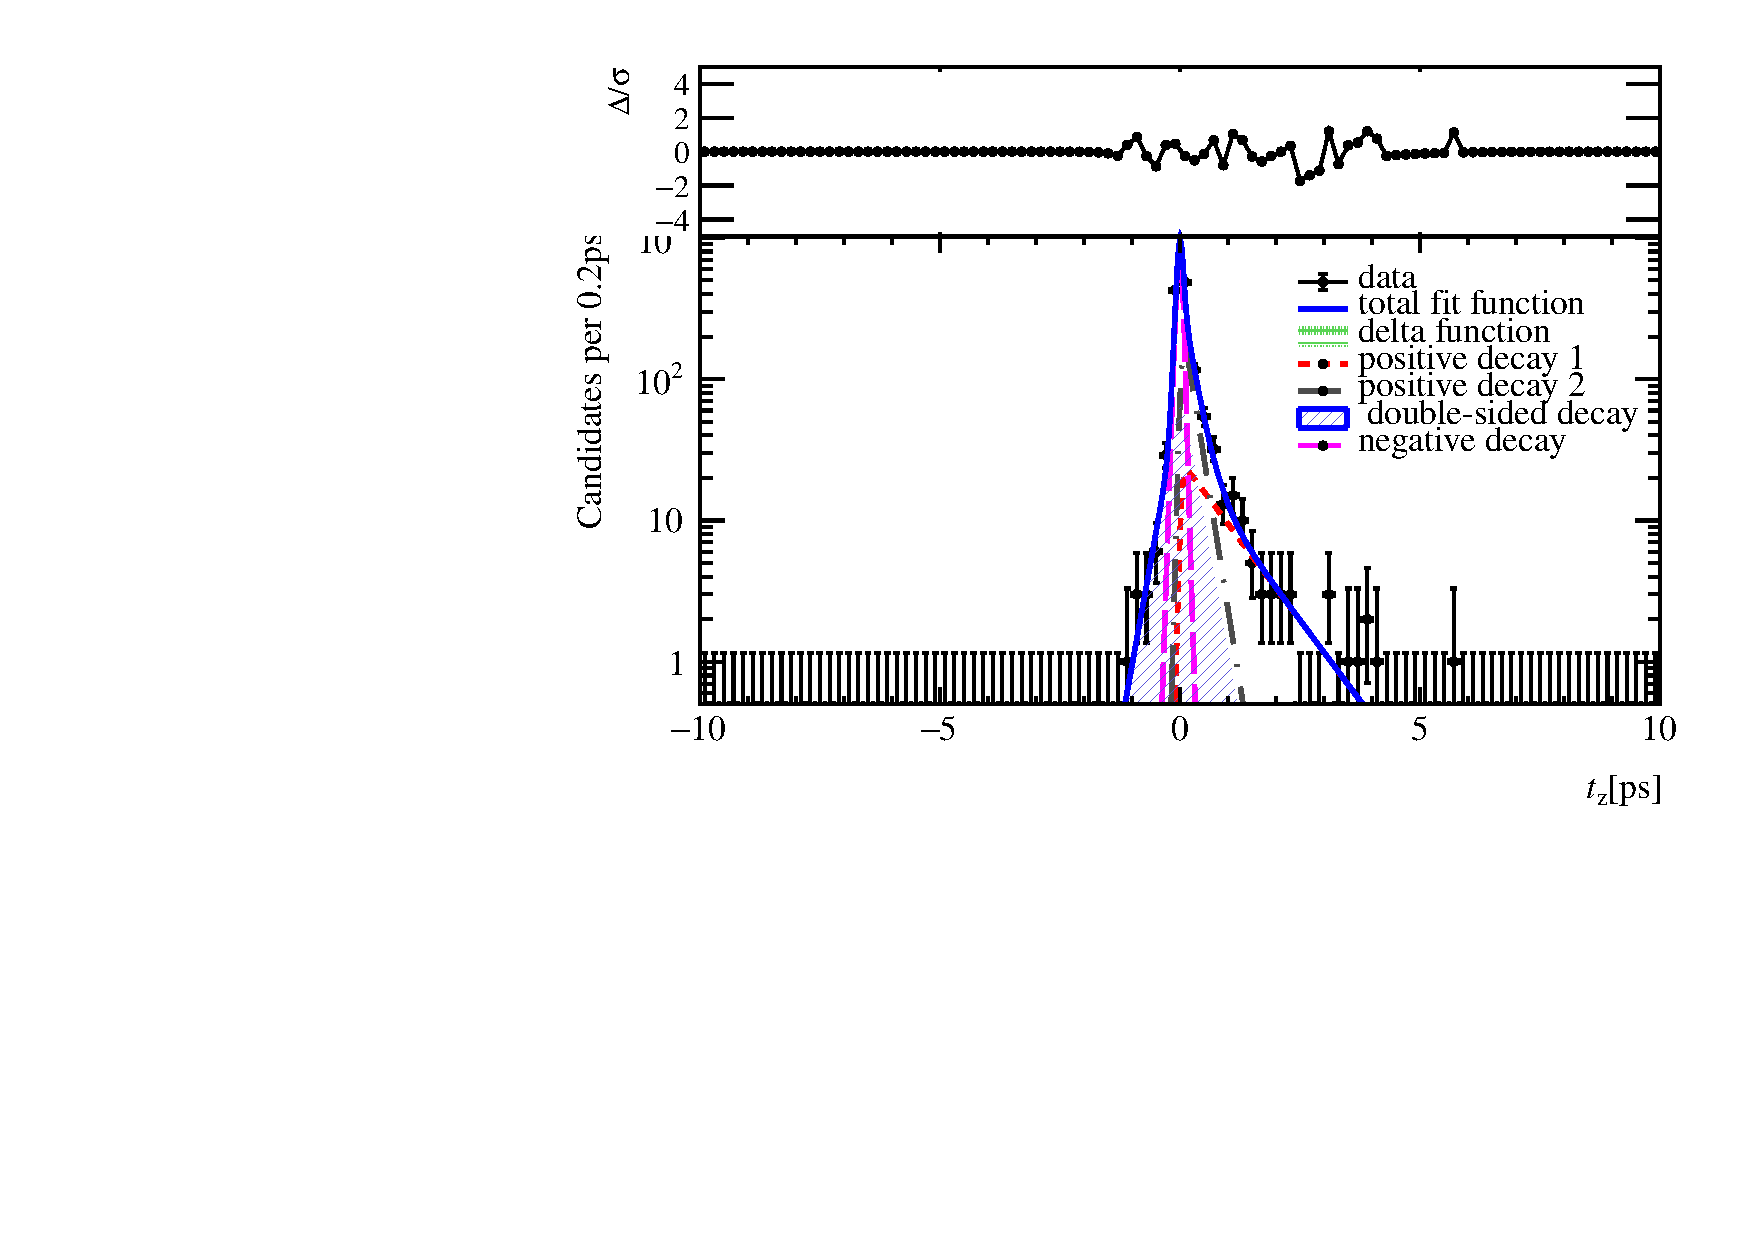
\includegraphics[width=0.49\linewidth]{pdf/pPb/Workdir/TzbkgFit/Psi2S_n1y1pt1.pdf}
\end{center}
\caption{
	$t_z$ background fit for \jpsi (left) and \psitwos (right) for $4\leq N_{\rm tracks}^{\rm PV} < 45$ in $p$Pb configuration.}
\label{fig_tzbkg}
\end{figure}
\begin{figure}[!tbp]
\begin{center}
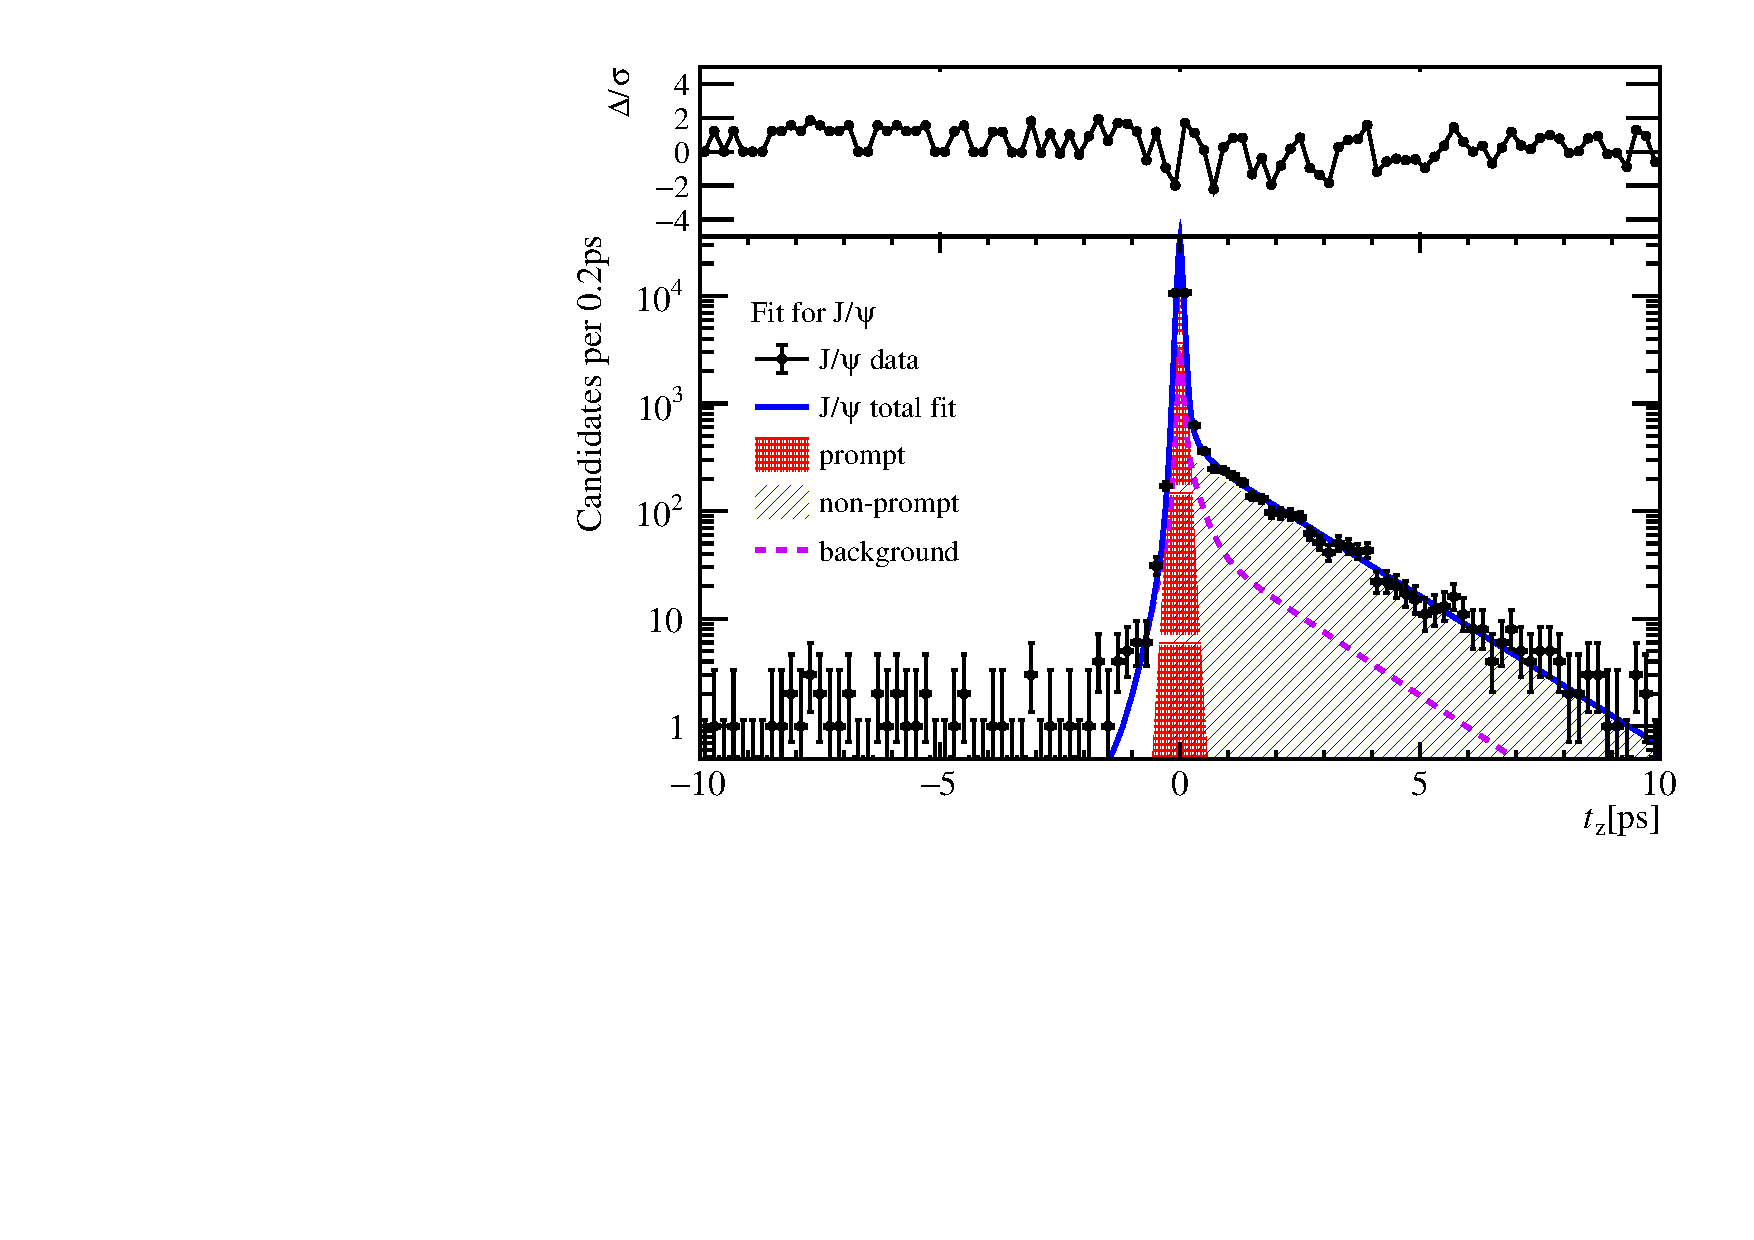
\includegraphics[width=0.49\linewidth]{pdf/pPb/Workdir/TwoDimFit/ProjTz/Jpsi_n1y1pt1.pdf}
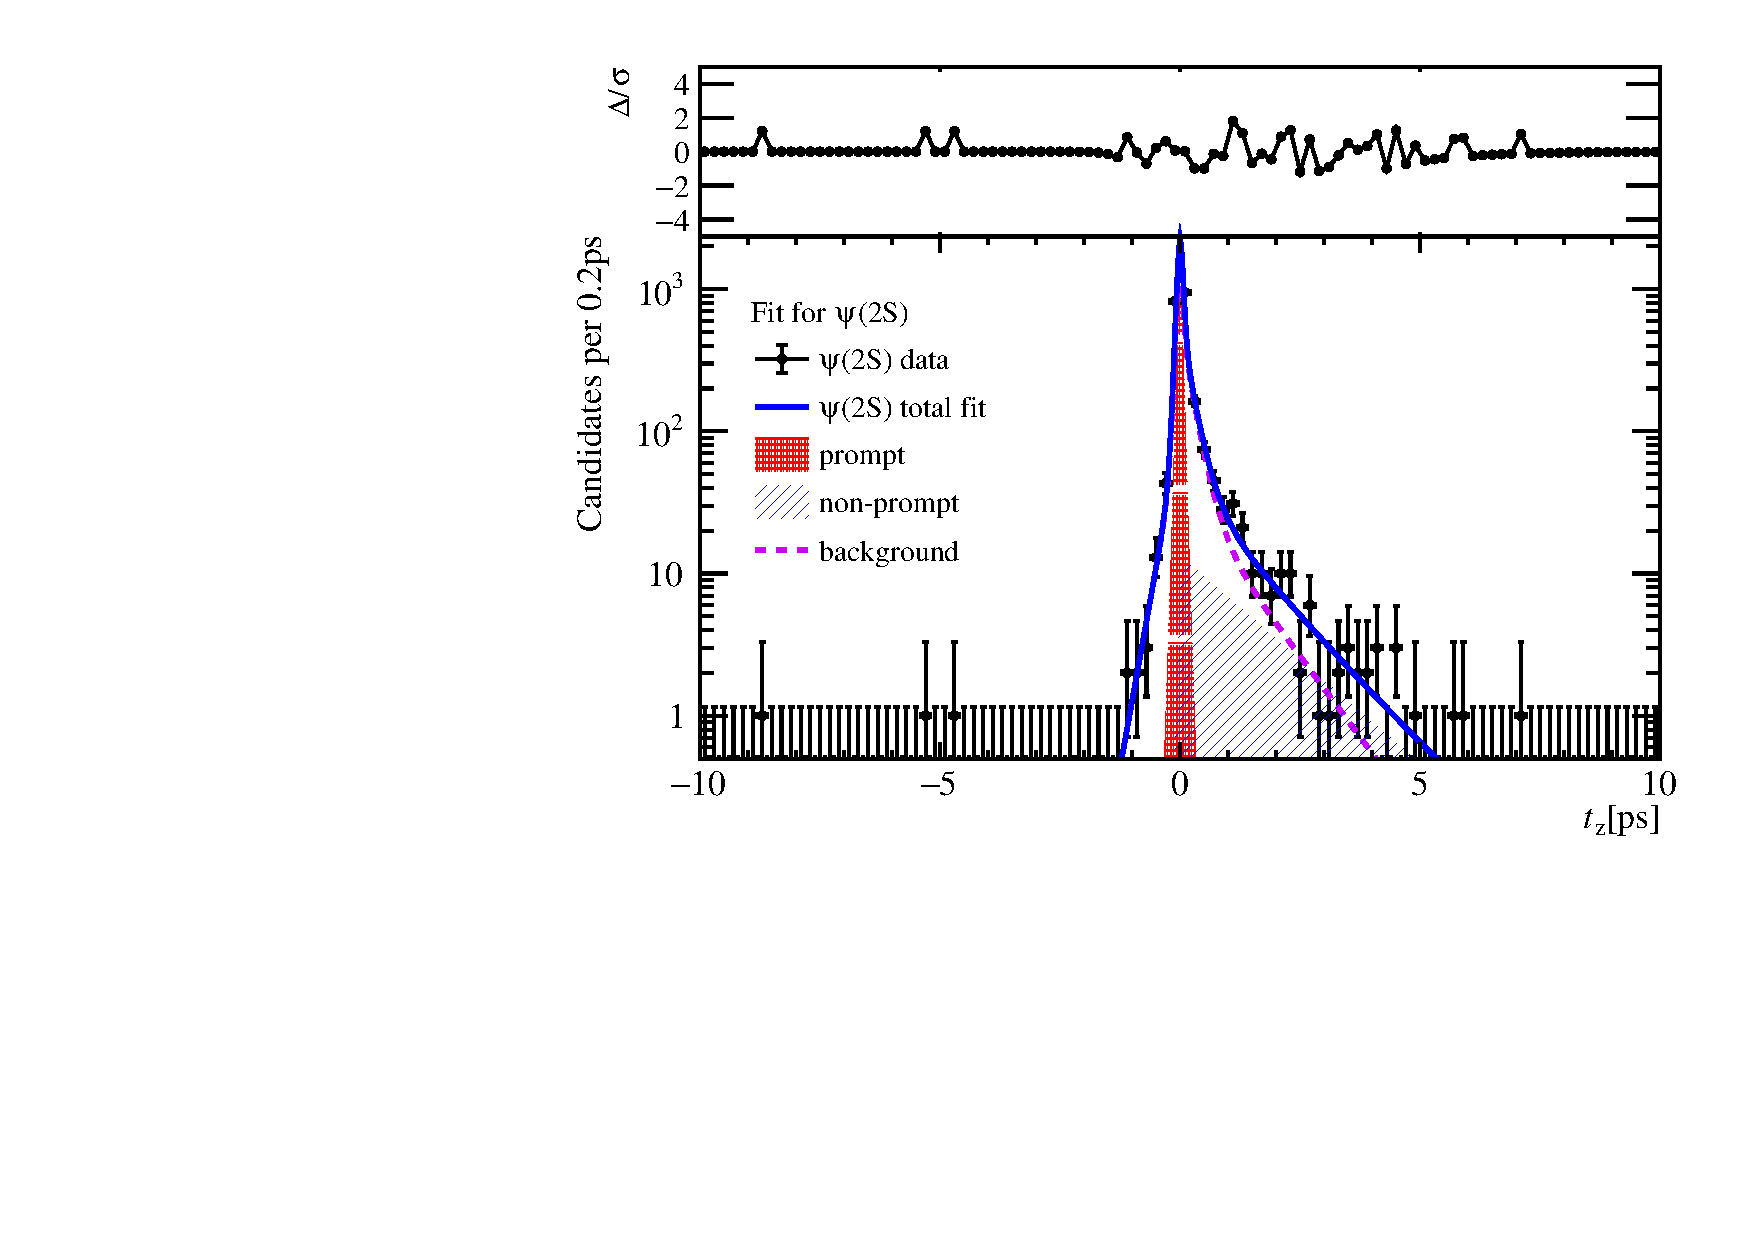
\includegraphics[width=0.49\linewidth]{pdf/pPb/Workdir/TwoDimFit/ProjTz/Psi2S_n1y1pt1.pdf}
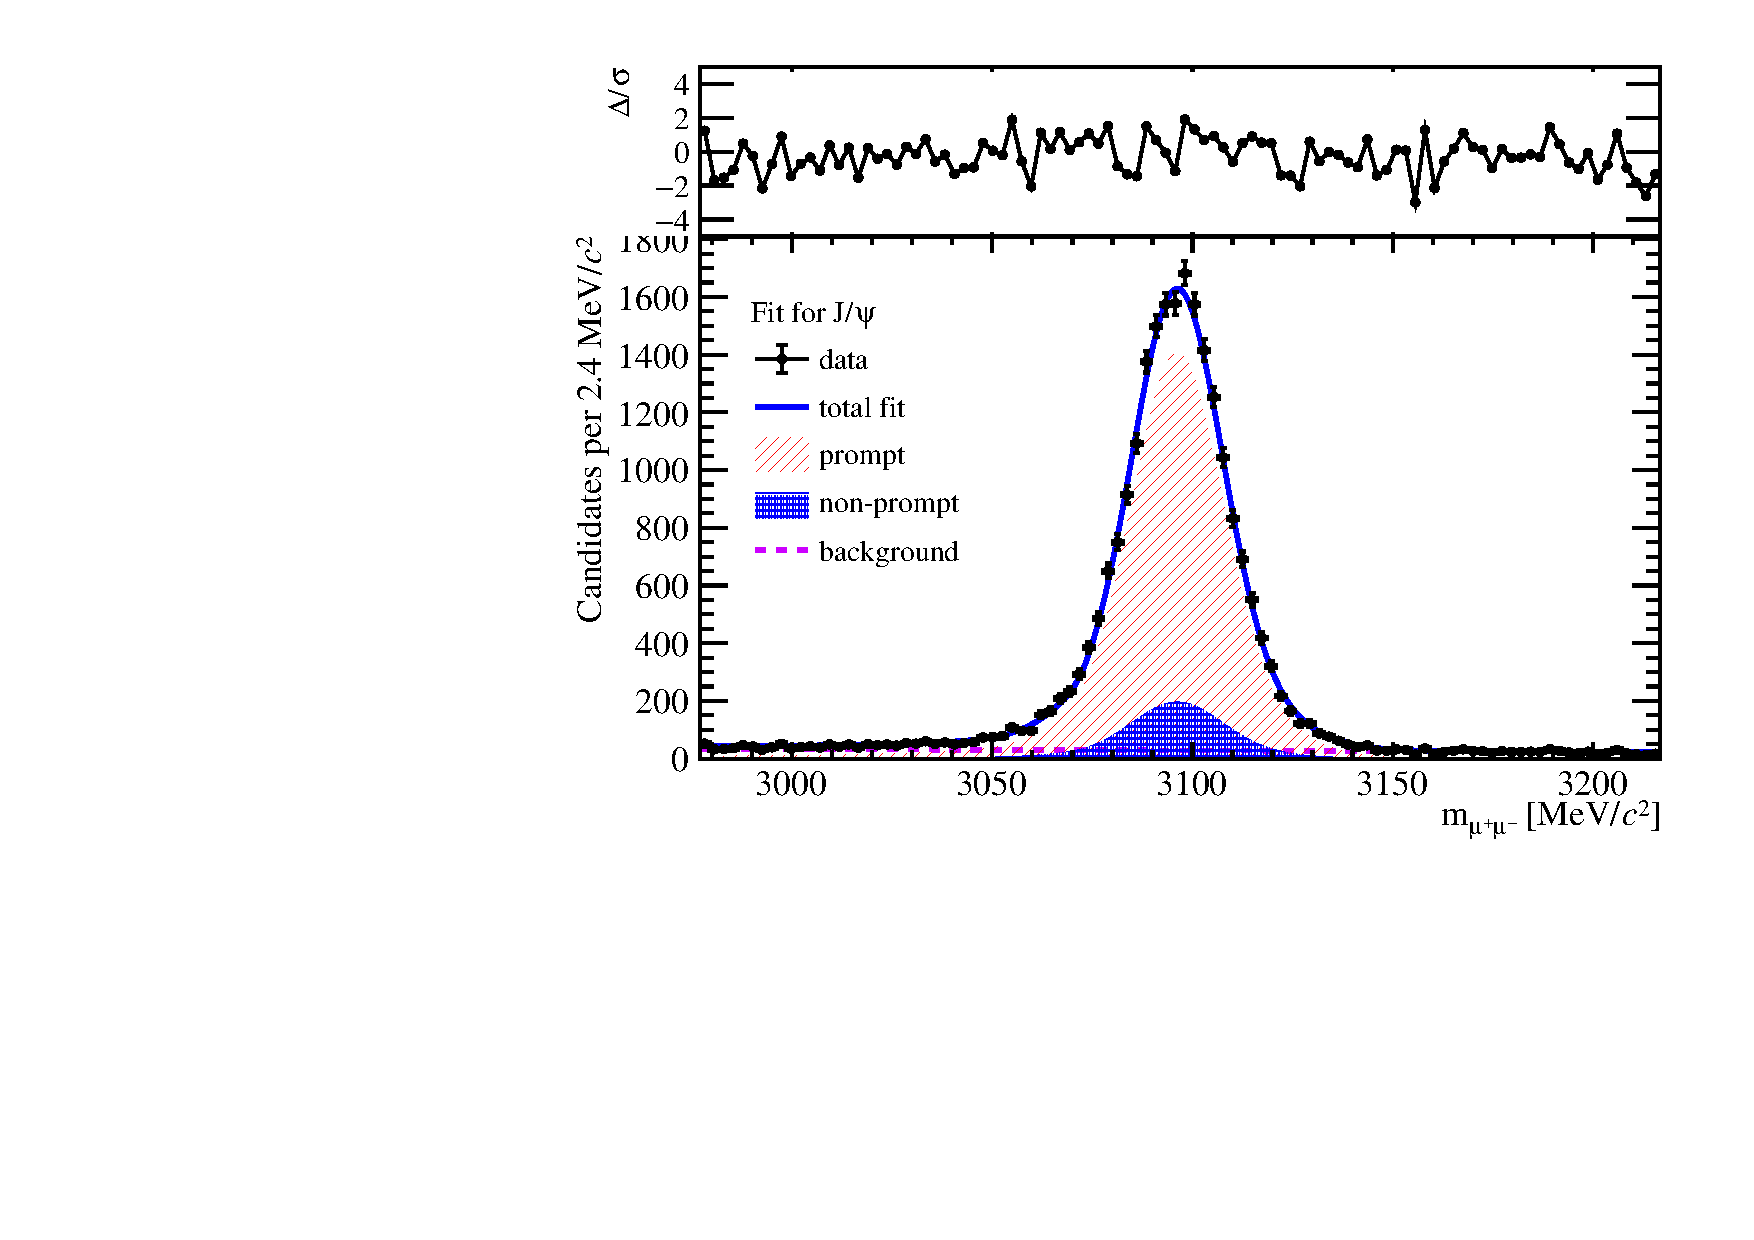
\includegraphics[width=0.49\linewidth]{pdf/pPb/Workdir/TwoDimFit/ProjMass/Jpsi_n1y1pt1.pdf}
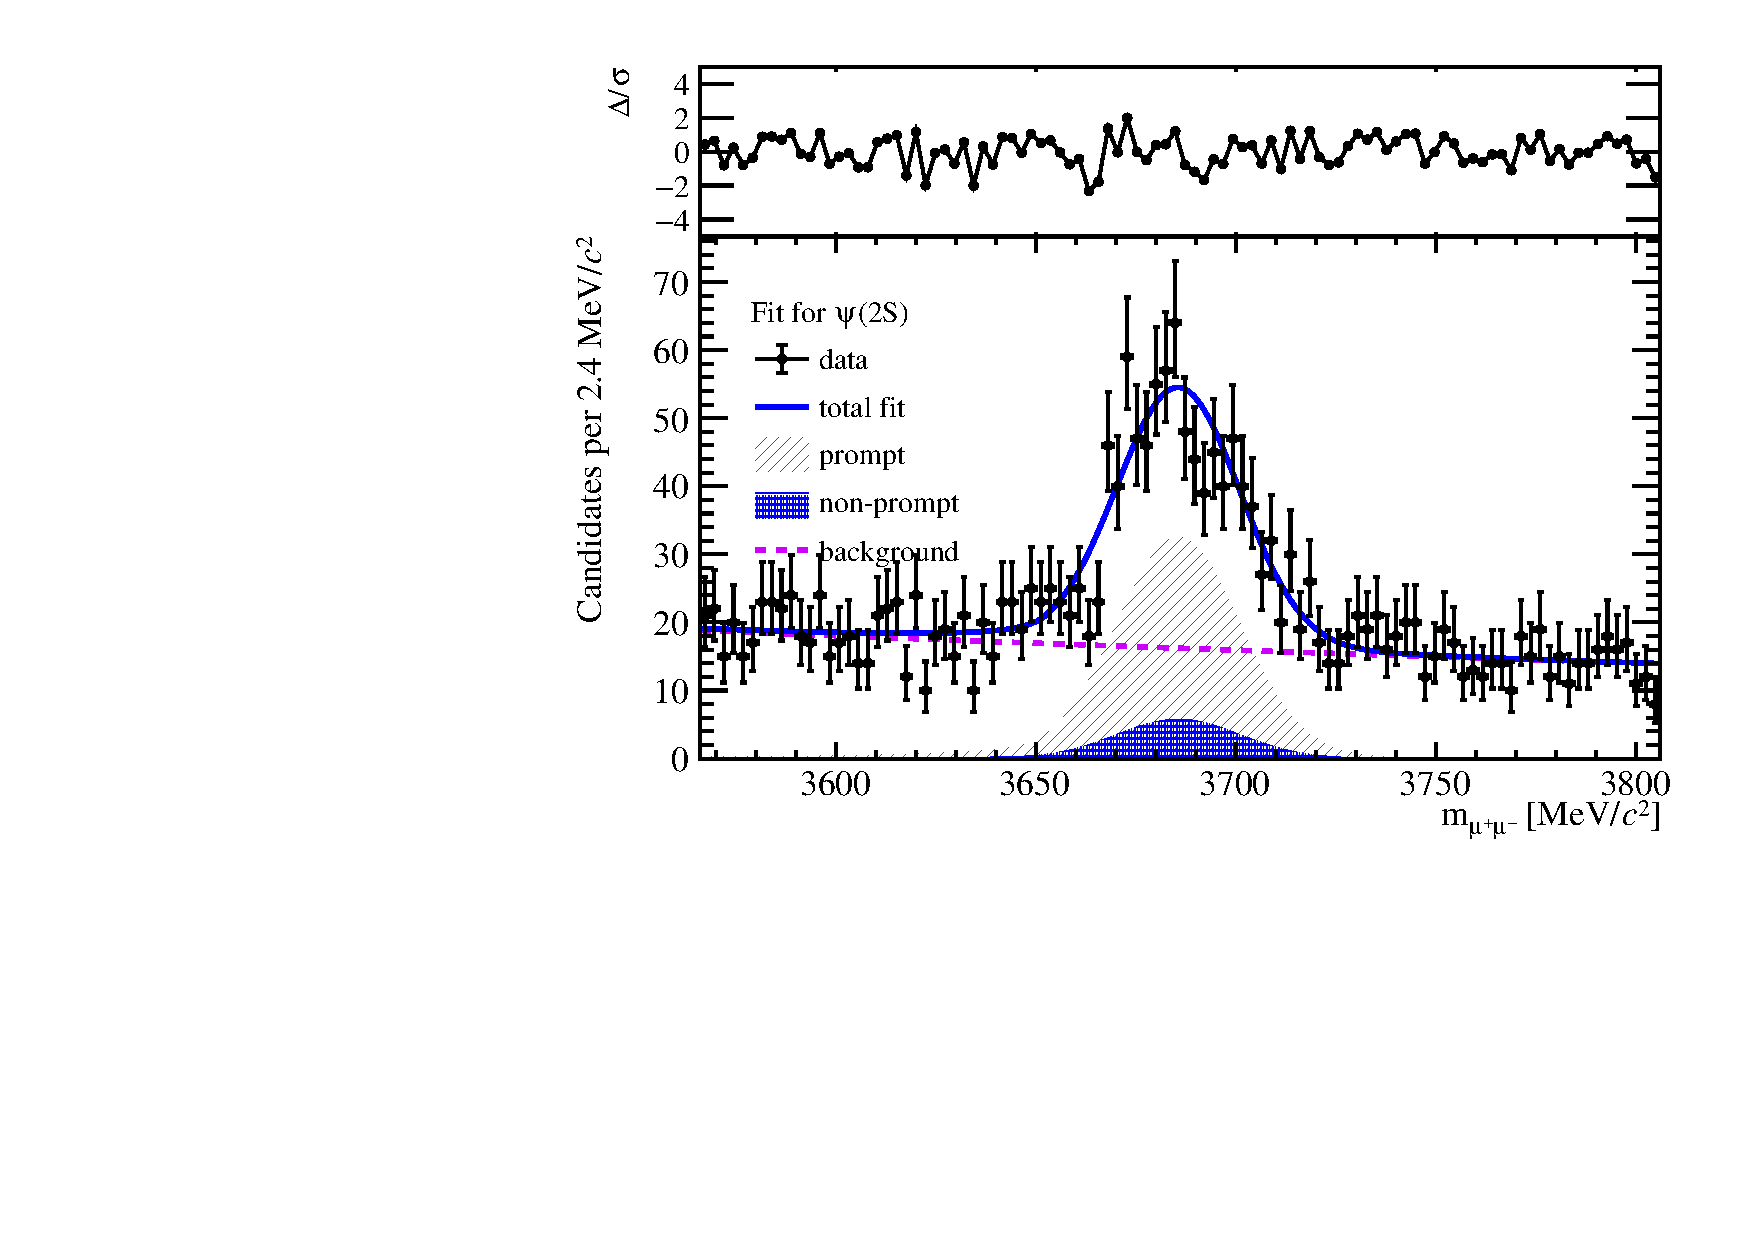
\includegraphics[width=0.49\linewidth]{pdf/pPb/Workdir/TwoDimFit/ProjMass/Psi2S_n1y1pt1.pdf}
\end{center}
\caption{
	2-Dimensional fit projected on $t_z$ spectrum (first row)  and mass spectrum (second row) for \jpsi (left) and \psitwos (right) for $4\leq N_{\rm tracks}^{\rm PV} < 45$ in $p$Pb configuration.}
\label{fig_2DFit}
\end{figure}





%%%%%%%%%%%%%%%%%%%%%%%%%%%%%%%%%%%%%%%%%%%%%%%%%%%%%%%%%%%%%%%%%%%%%%%Efficiency%%%%%%%%%%%%%%%%%%%%%%%%%%%%%%%%%%%%%%%%%%%%%%%%%%%%%%%%%%%%%%%%%%%%%%%%%%%%%%%%%%%%%%%%
\section{Efficiency determination}
\label{Efficiency determination}
The number of signal candidates are corrected by the total efficiency to obtain the \psitwos-to-\jpsi cross-section ratio measurements. The efficiencies are assumed to be equal for prompt and from-$b$ signals as can be seen for example in the measurement of \jpsi cross-section at 13 TeV~\cite{LHCb-PAPER-2015-037}. The total efficiency is the product of the acceptance efficiency (\effAcc), the reconstruction and selection efficiency (\effReco), the particle identification efficiency (\effID), and the trigger efficiency (\effTrigger). The acceptance efficiency is calculated for all multiplicity classes. The others are calculated in each multiplicity class. And according to Eq.~\ref{CS_ratio}, we are going to find the efficiency ratio in each multiplicity class. The ratio of total efficiencies for \jpsi and \psitwos is defined in the following equation~\ref{EffRatio}.
\begin{equation}
\begin{split}
R_{tot}=&\frac{\ensuremath{\epsilon_{\mathrm{tot,\jpsi}}}}{\ensuremath{\epsilon_{\mathrm{tot,\psitwos}}}}\bigg|_{Mult. \ bin} \\
= &\frac{\ensuremath{\epsilon_{\mathrm{acc,\jpsi}}}}{\ensuremath{\epsilon_{\mathrm{acc,\psitwos}}}}\times \frac{\ensuremath{\epsilon_{\mathrm{Reco\&Sel,\jpsi}}}\cdot\ensuremath{\epsilon_{\mathrm{MuonID,\jpsi}}}\cdot\ensuremath{\epsilon_{\mathrm{Trigger,\jpsi}}}}{\ensuremath{\epsilon_{\mathrm{Reco\&Sel,\psitwos}}}\cdot\ensuremath{\epsilon_{\mathrm{MuonID,\psitwos}}}\cdot\ensuremath{\epsilon_{\mathrm{Trigger,\psitwos}}}}\bigg|_{Mult. \ bin} \\
= &R_{acc}\times R_{eff}|_{Mult. \ bin},
\end{split}
\label{EffRatio}
\end{equation}
where $R_{acc}$ is the ratio of acceptance efficiencies of \jpsi to \psitwos and $R_{eff}$ is the ratio of the remaining efficiencies of \jpsi and \psitwos. 
All steps are determined from simulation, with truth matched signal decays, except for the tracking efficiency and the particle identification, where data driven methods are used to correct the efficiencies obtained from the simulation. Their exact definitions are given in the following subsections. In the simulation, \jpsi and \psitwos mesons are assumed produced without polarization. For the simulation samples used for this analysis, the truth matching efficiency is equal to $99.5 \pm 0.1\%$ for both $p$Pb and Pb$p$ samples. It is assumed to be independent of \pt and $y^*$.

\subsection{Re-weight on Monte Carlo sample}
\label{reweight}
\subsubsection{Multiplicity distribution}
Even though the simulated sample used here is multiplicity-fixed sample, which is introduced in Sec~\ref{subsecMC}, there are still differences between the multiplicity distribution in simulated samples and data. Before calculating efficiencies using the simulated sample, we need to reweight the multiplicity distribution in simulated sample to match that in signal sample extracted from data by sPlot method~\cite{Pivk:2004ty}. However, due to the small statistics for \psitwos sample, the reweight on multiplicity can introduce large systematic uncertainty. When the variation in the ratio of efficiency caused by the difference in multiplicity distribution is small, there is no reason to introduce a large uncertainty for it. To see whether the reweight on multiplicity has a huge effect on efficiency ratio, we can compare the distribution in simulated sample and signal sample. If the multiplicity distributions for \jpsi and \psitwos are almost the same in simulated sample and signal sample, we can conclude that, the weight in each multiplicity bin is the same, then when calculating the ratio of efficiency, the variation caused by the differences in simulated and signal sample is expected to cancel.

The distribution of $N_{\rm tracks}^{\rm PV}$, $N_{\rm fwd}^{\rm PV}$ and $N_{\rm bwd}^{\rm PV}$ of simulated and signal sample for both \jpsi and \psitwos in $p$Pb and Pb$p$ configurations are compared. As an example, we draw the distributions for simulated and signal sample in $p$Pb configuration in Figure~\ref{MulReweight}. We can see that the multiplicity distribution for \jpsi and \psitwos signals both in simulated and signal sample are compatible within uncertainties. And what we want in the end is the ratio of total efficiencies. The bias in the ratio of efficiency caused by the difference in multiplicity should be canceled.
\begin{figure}[H]
\begin{center}
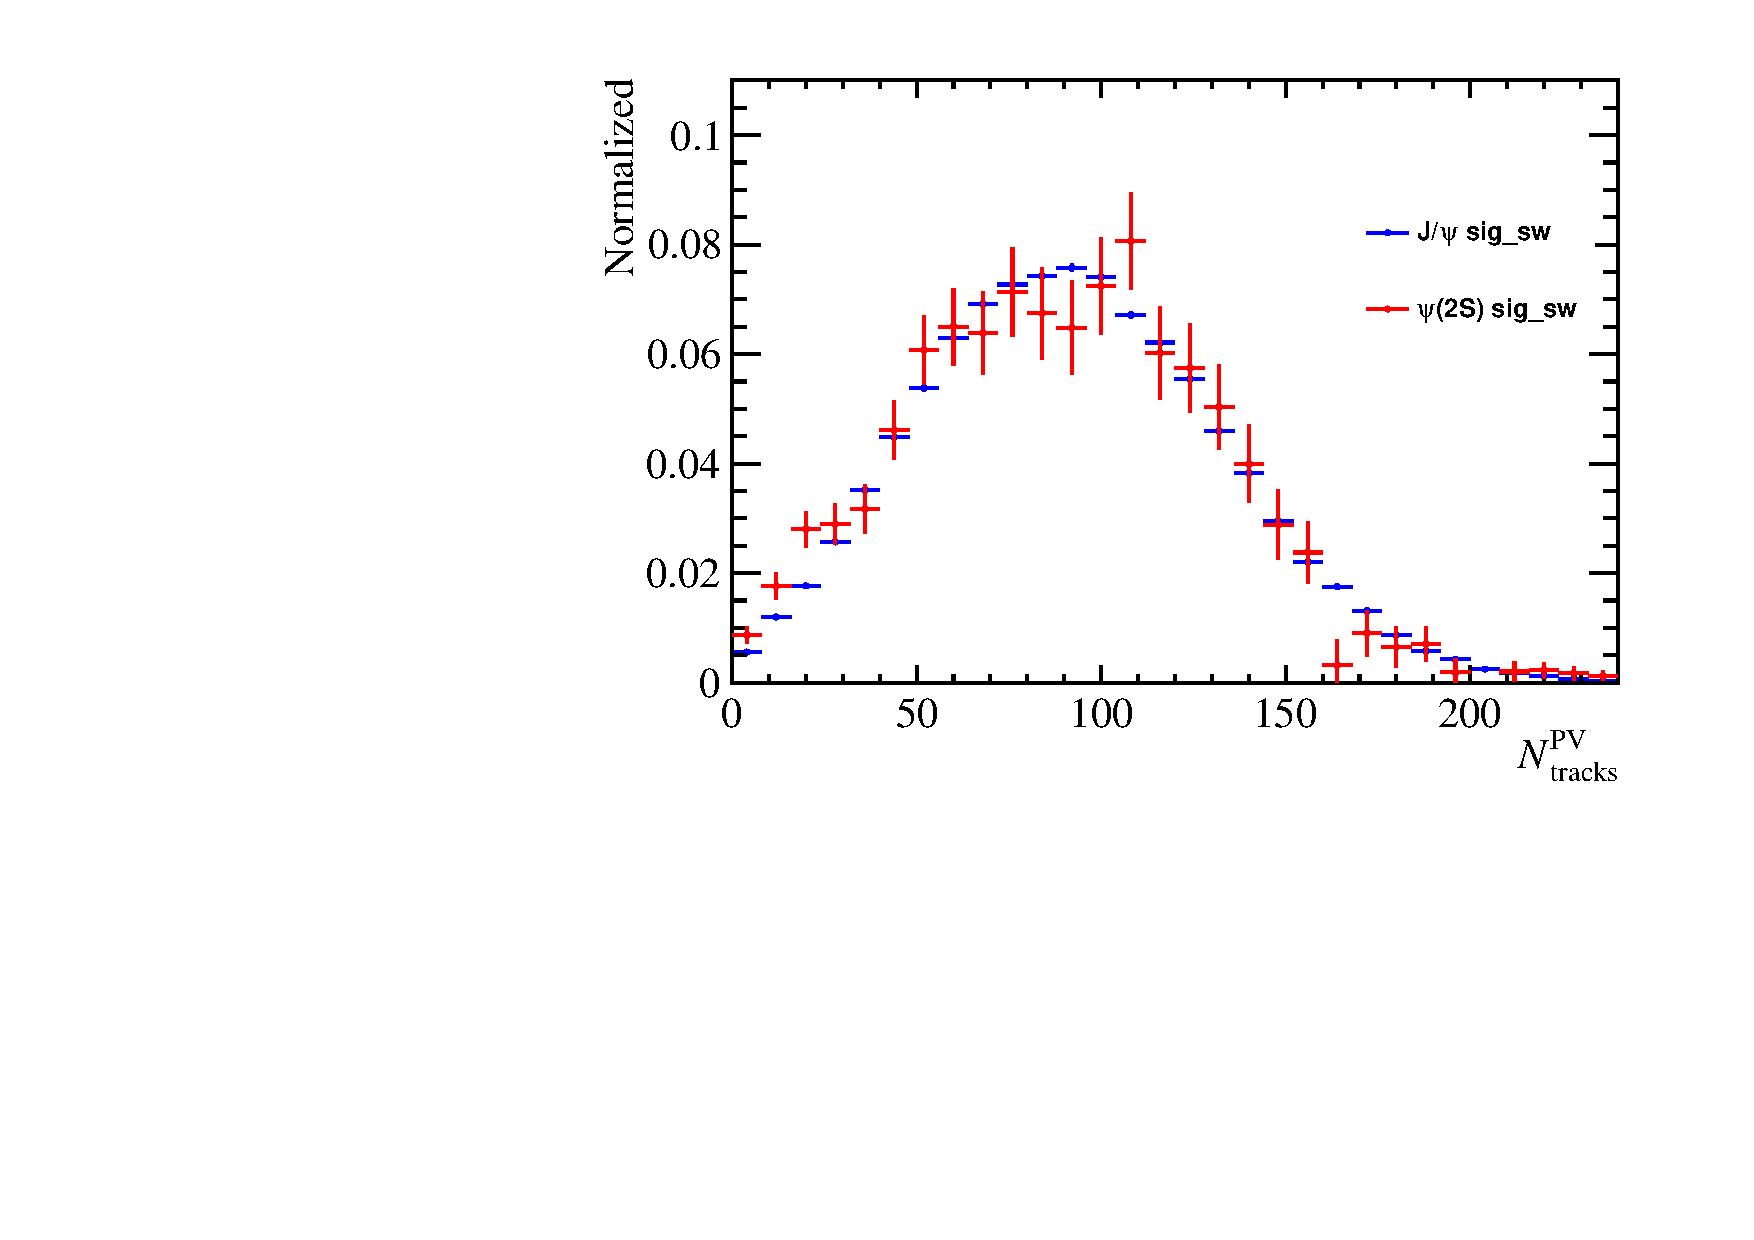
\includegraphics[width=0.32\linewidth]{pdf/pPb/Workdir/Reweight/sWeightMul.pdf}
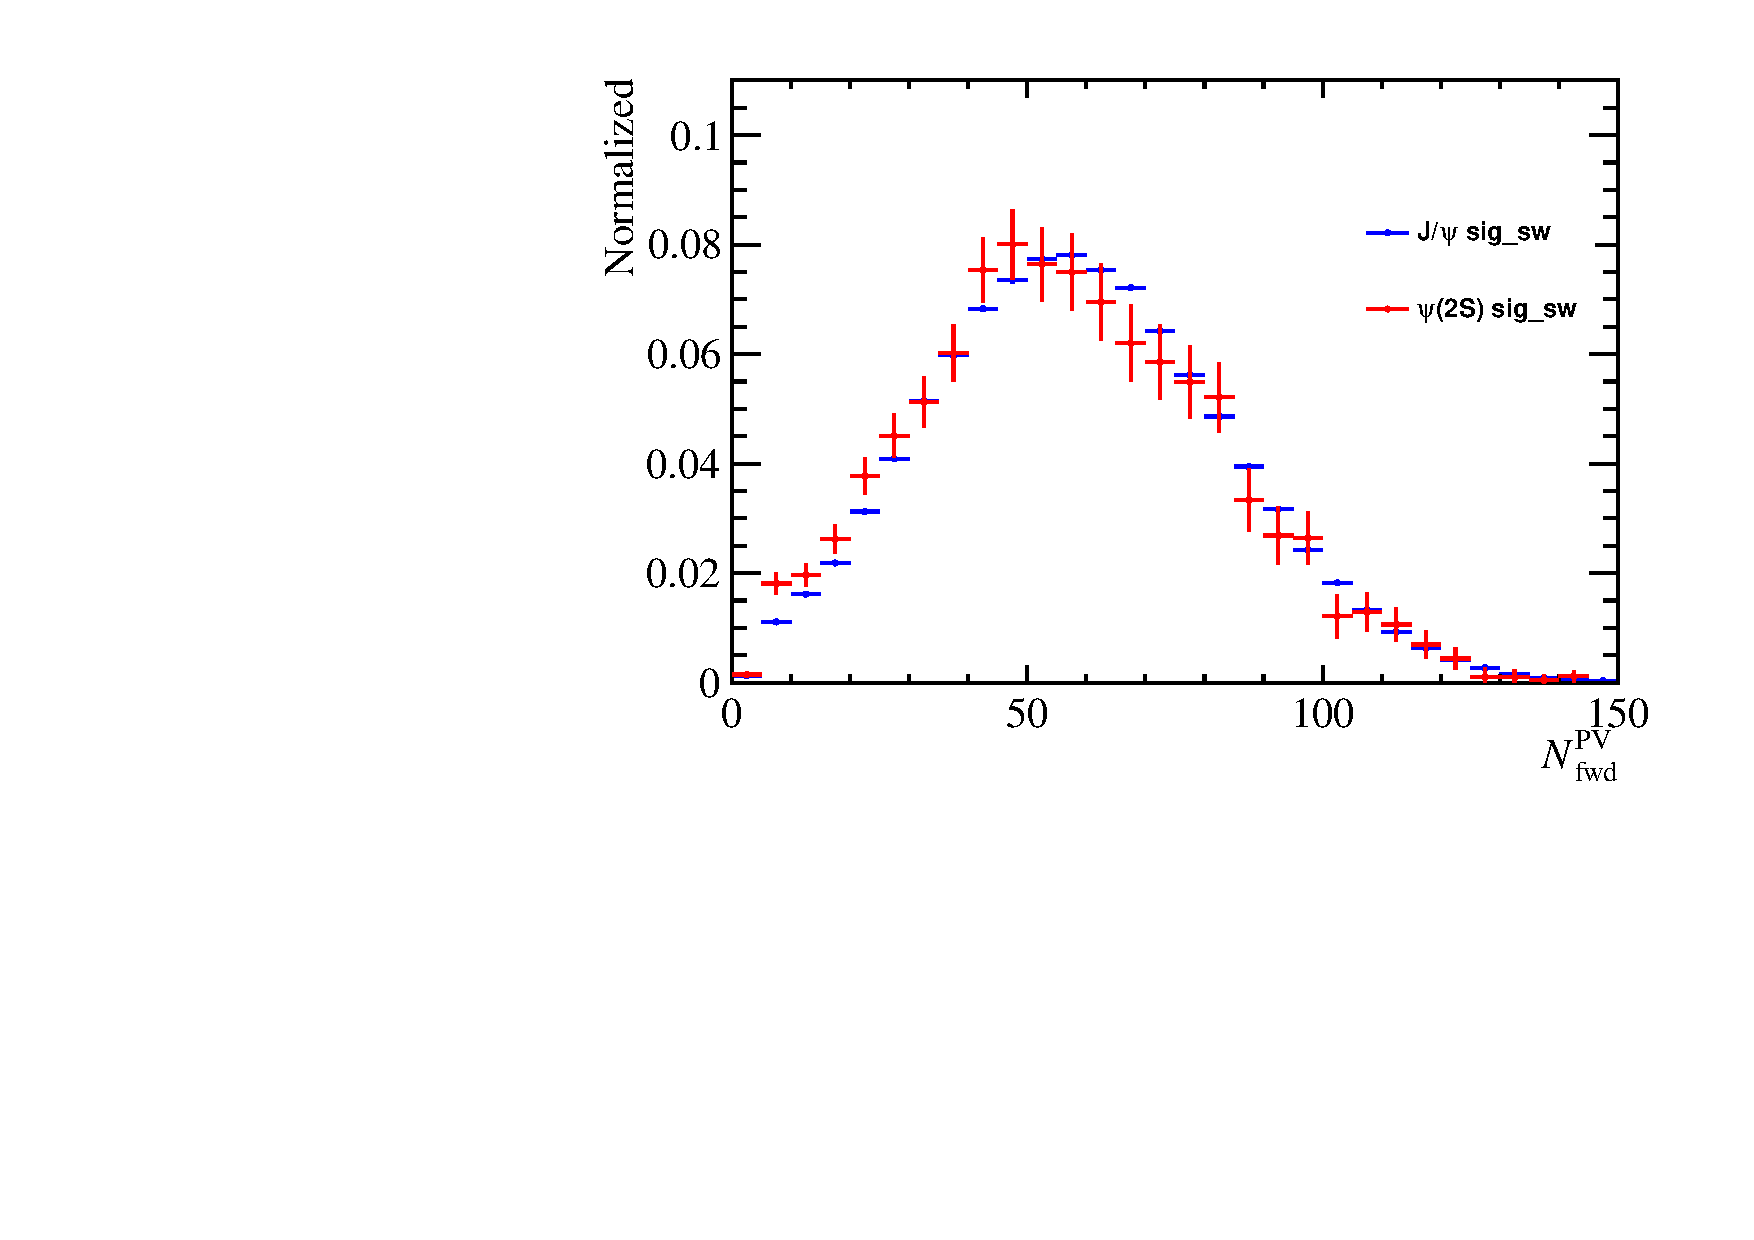
\includegraphics[width=0.32\linewidth]{pdf/pPb/FWorkdir/Reweight/sWeightMul.pdf}
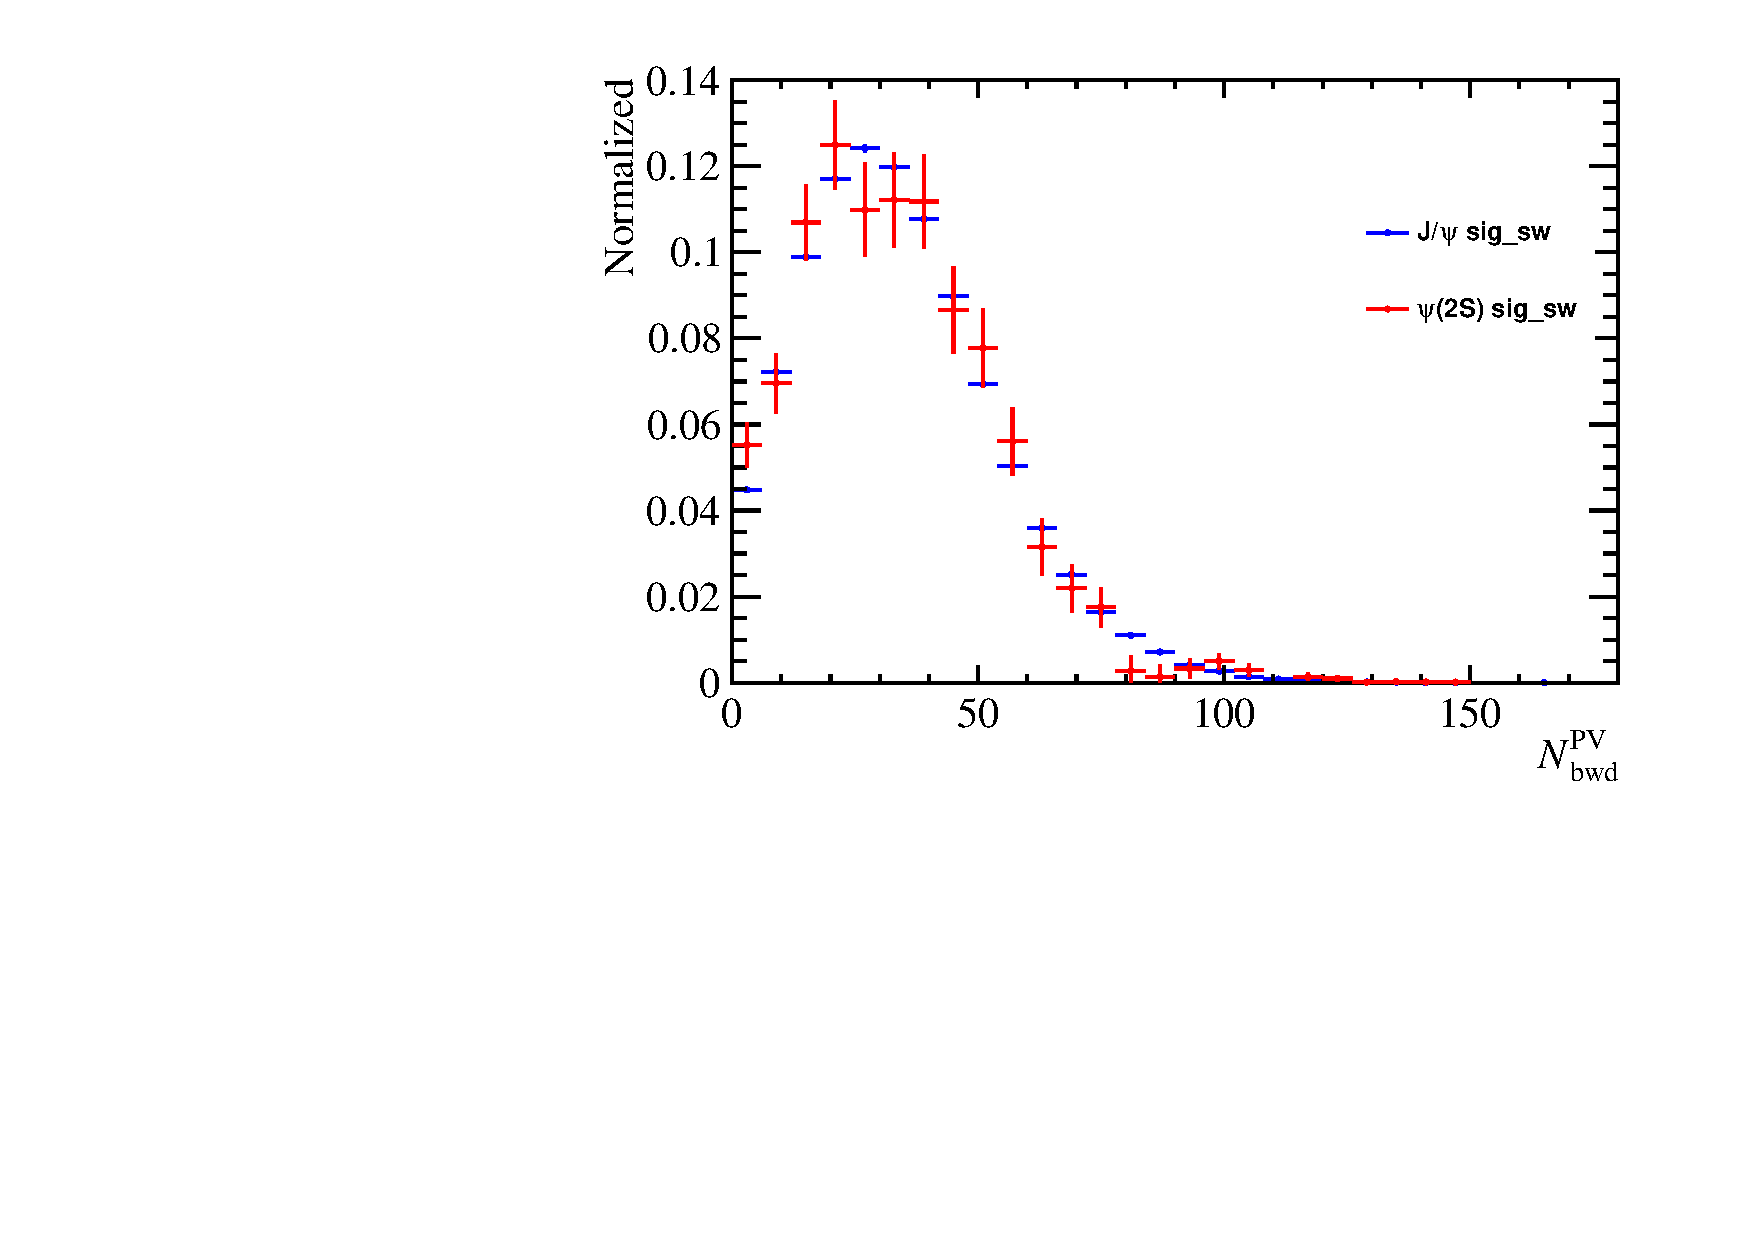
\includegraphics[width=0.32\linewidth]{pdf/pPb/BWorkdir/Reweight/sWeightMul.pdf}
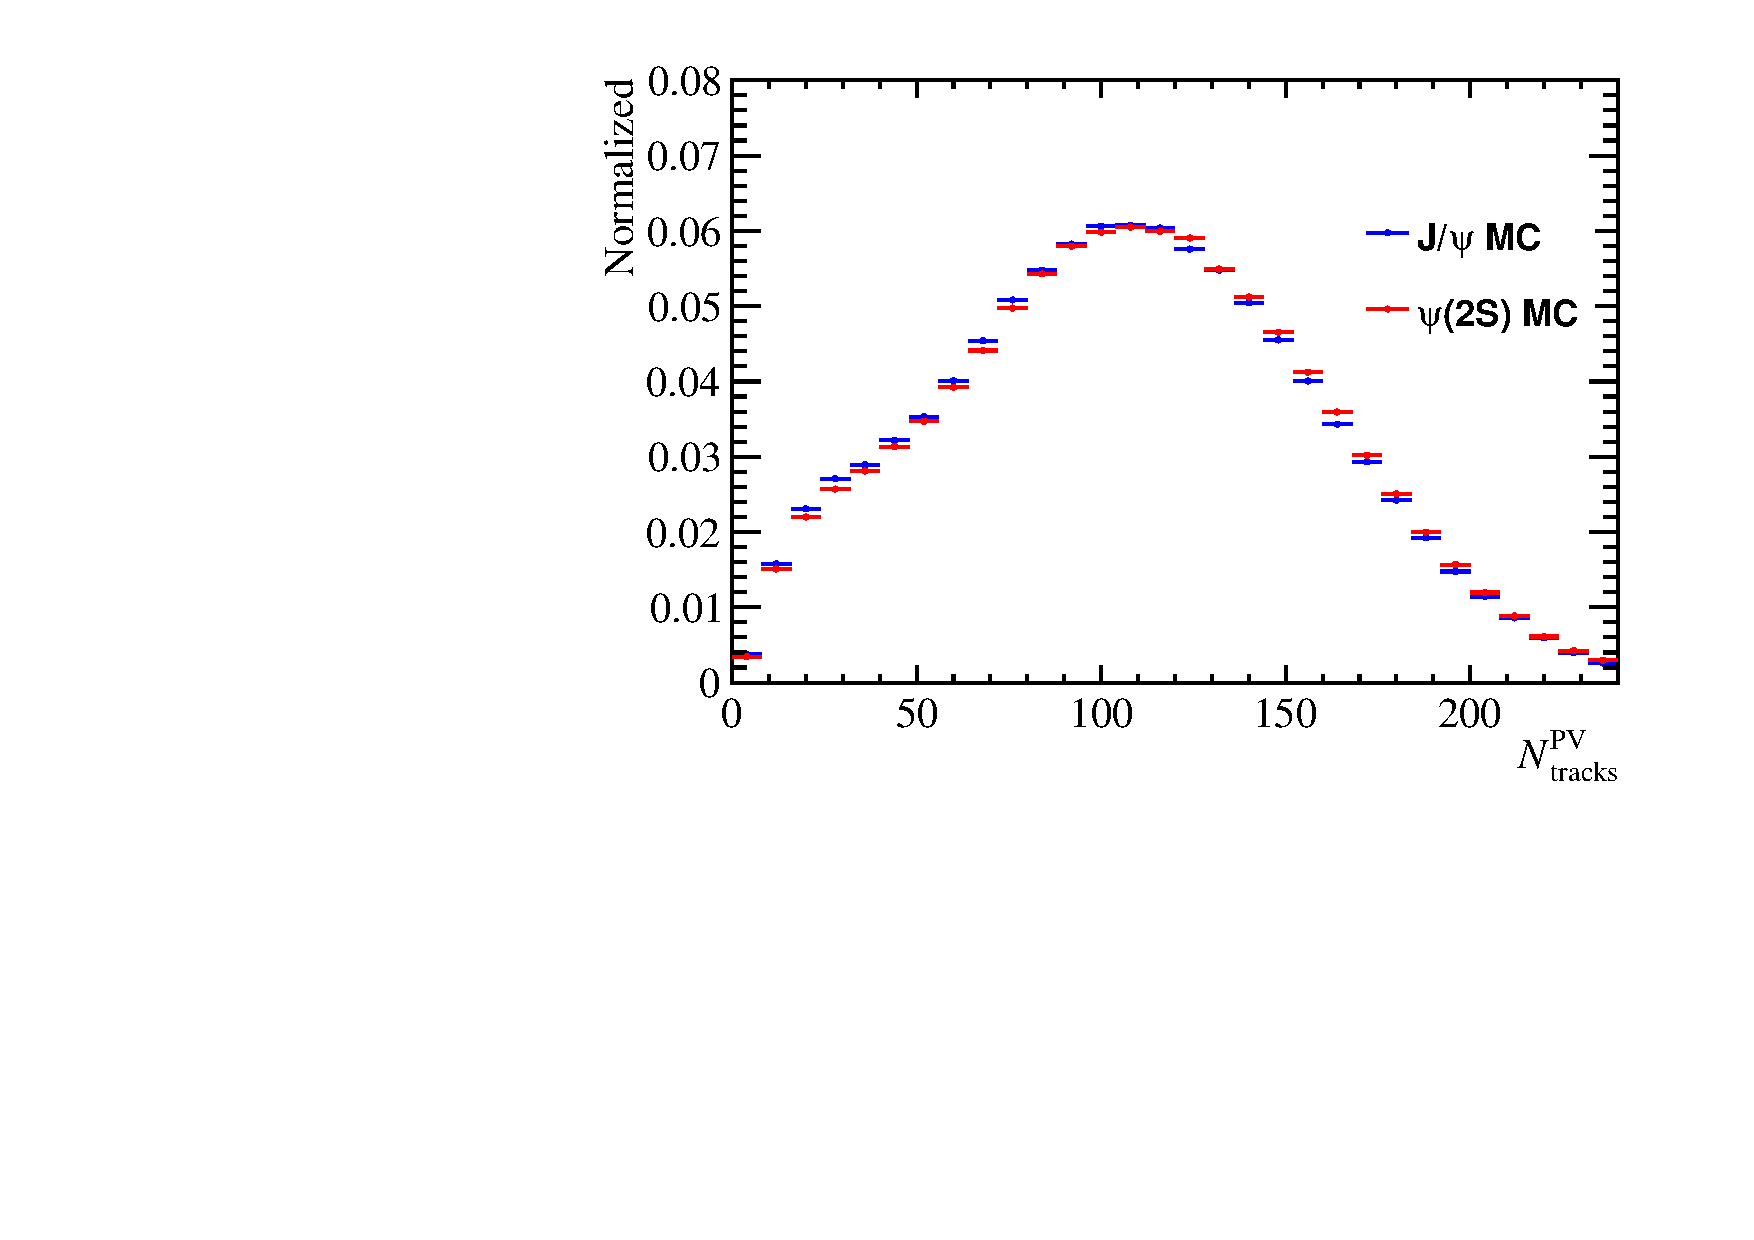
\includegraphics[width=0.32\linewidth]{pdf/pPb/Workdir/Reweight/MCMul.pdf}
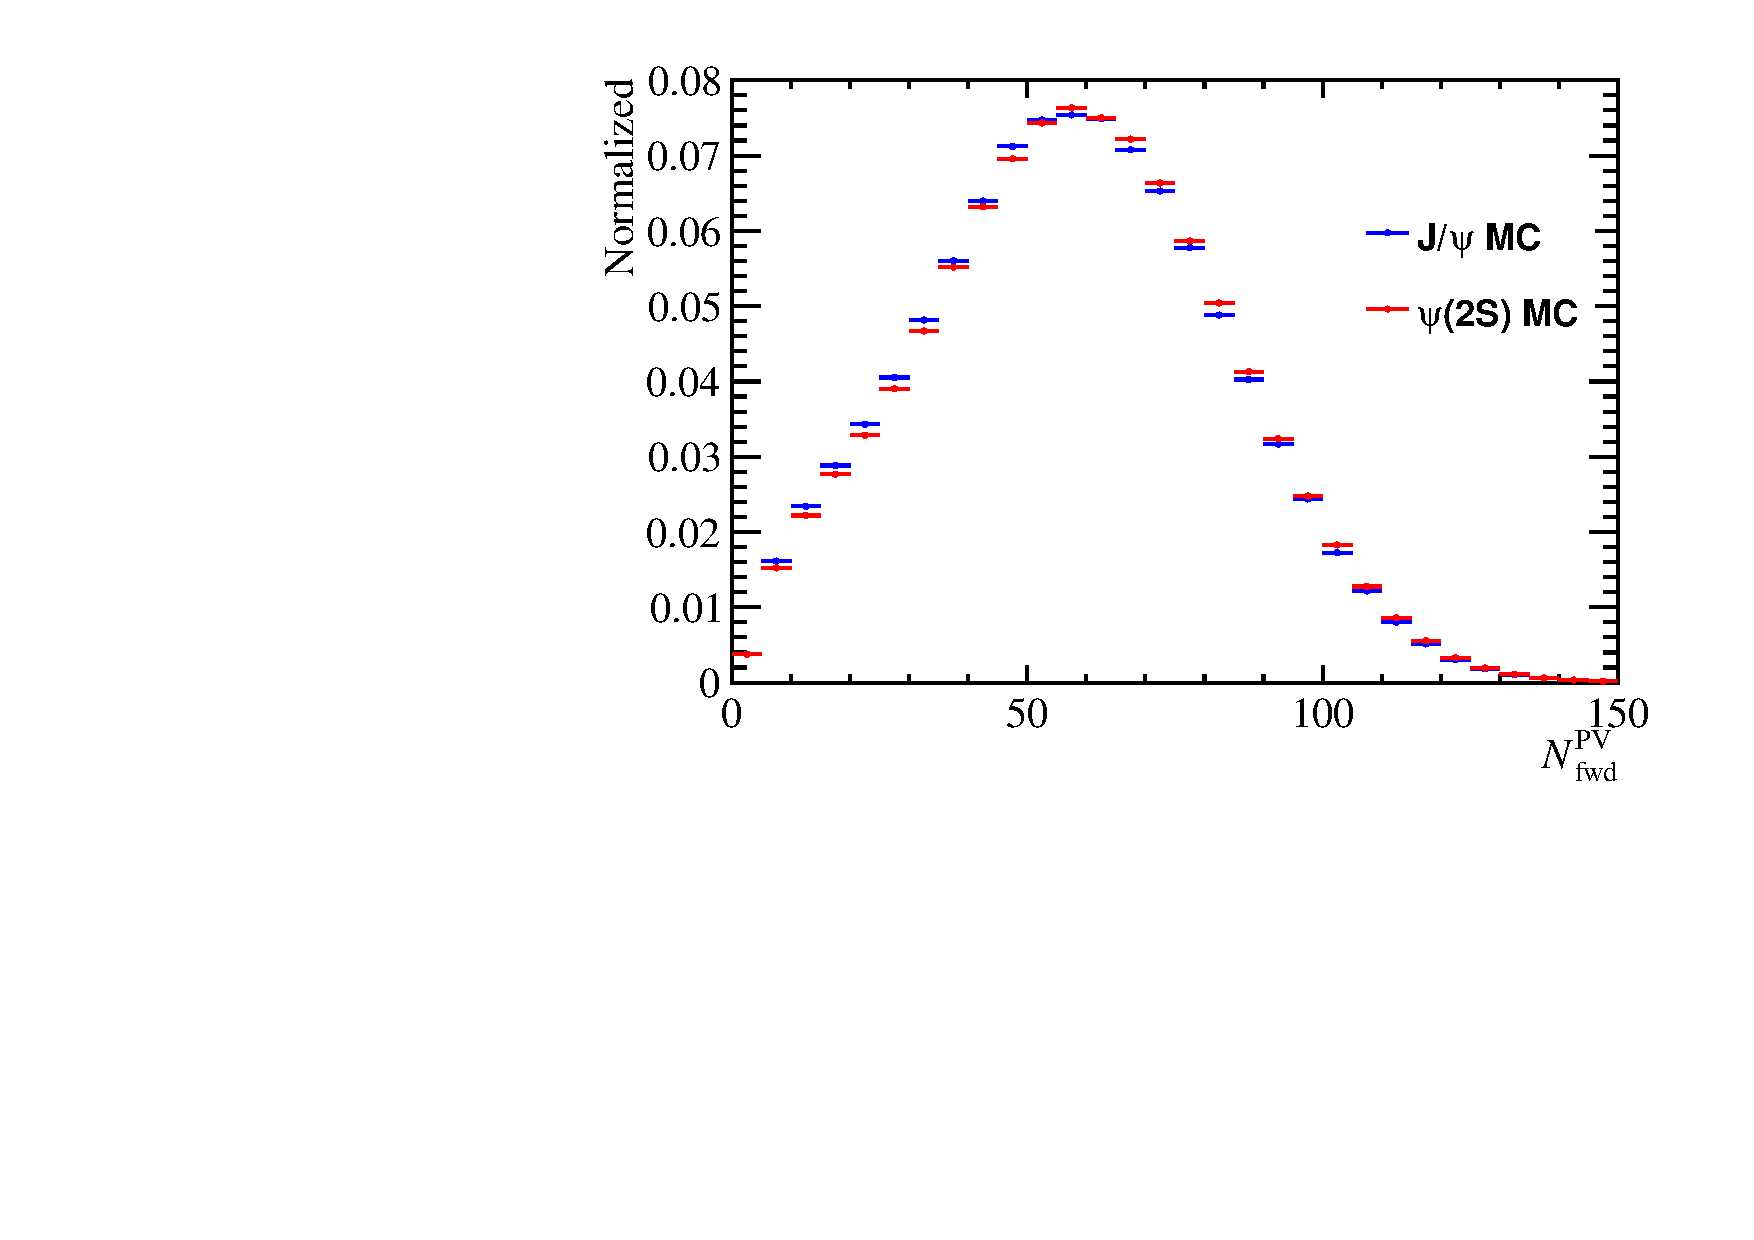
\includegraphics[width=0.32\linewidth]{pdf/pPb/FWorkdir/Reweight/MCMul.pdf}
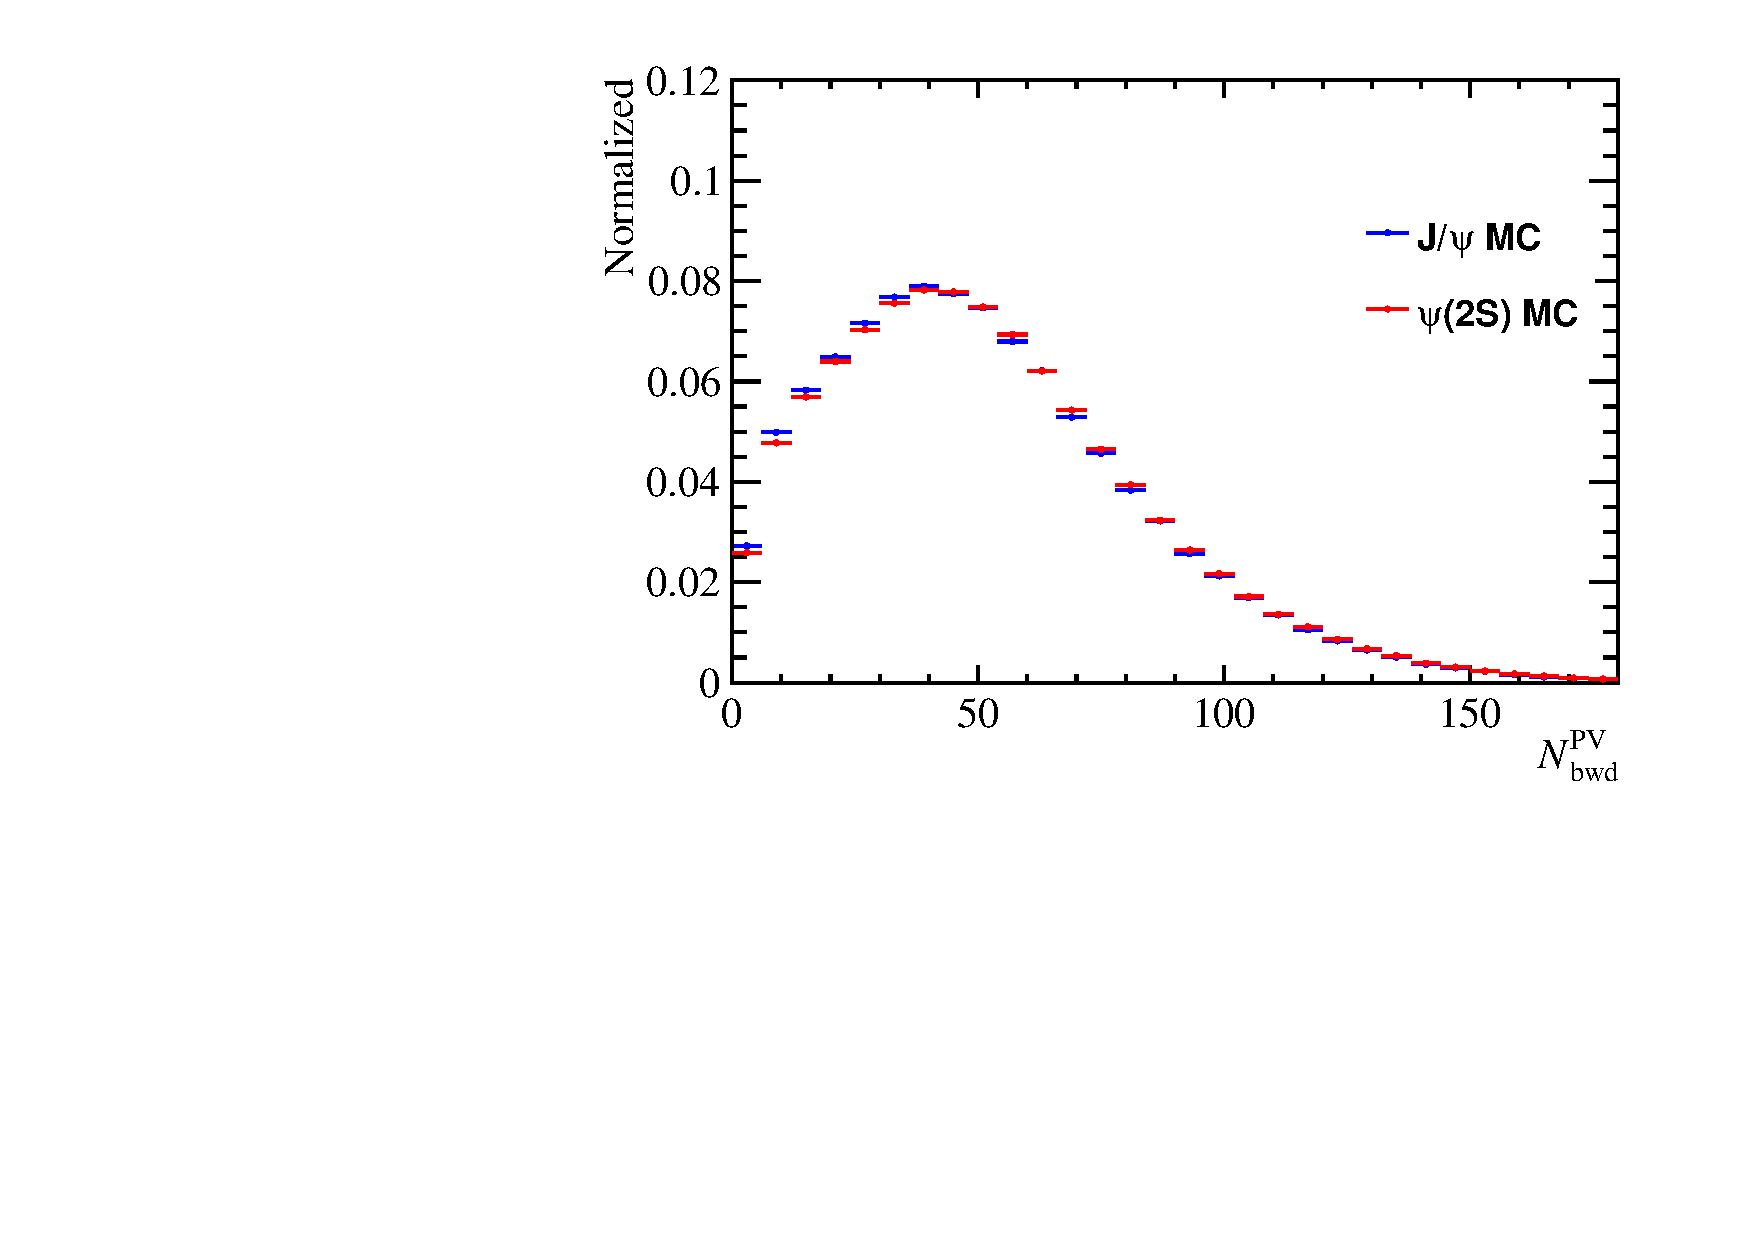
\includegraphics[width=0.32\linewidth]{pdf/pPb/BWorkdir/Reweight/MCMul.pdf}
\end{center}
\caption{
	Distribution of multiplicity variables for s-weight data (first row) and MC (second row) in $p$Pb configuration.}
\label{MulReweight}
\end{figure}

\subsubsection{\pt and $y$ distribution}
The differences in distribution of \pt and $y^*$ in simulated and signal samples are not negligible. Due to the fact that \pt and $y^*$ are slightly correlated to multiplicity, the reweight procedures are done in high- and low- multiplicity simulated and signal samples for both \jpsi and \psitwos. The high- and low-multiplicity samples are separated by the mean values of multiplicity variables in signal sample according to the multiplicity variable we used. As an example, the re-weight of \pt and $y^*$ for high- and low-multiplicity \jpsi samples when taking $N_{\rm tracks}^{\rm PV}$ as multiplicity variable is shown in Figure~\ref{PTYReweightJ}. And that for \psitwos is shown in Figure~\ref{PTYReweightP}.
\begin{figure}[H]
\begin{center}
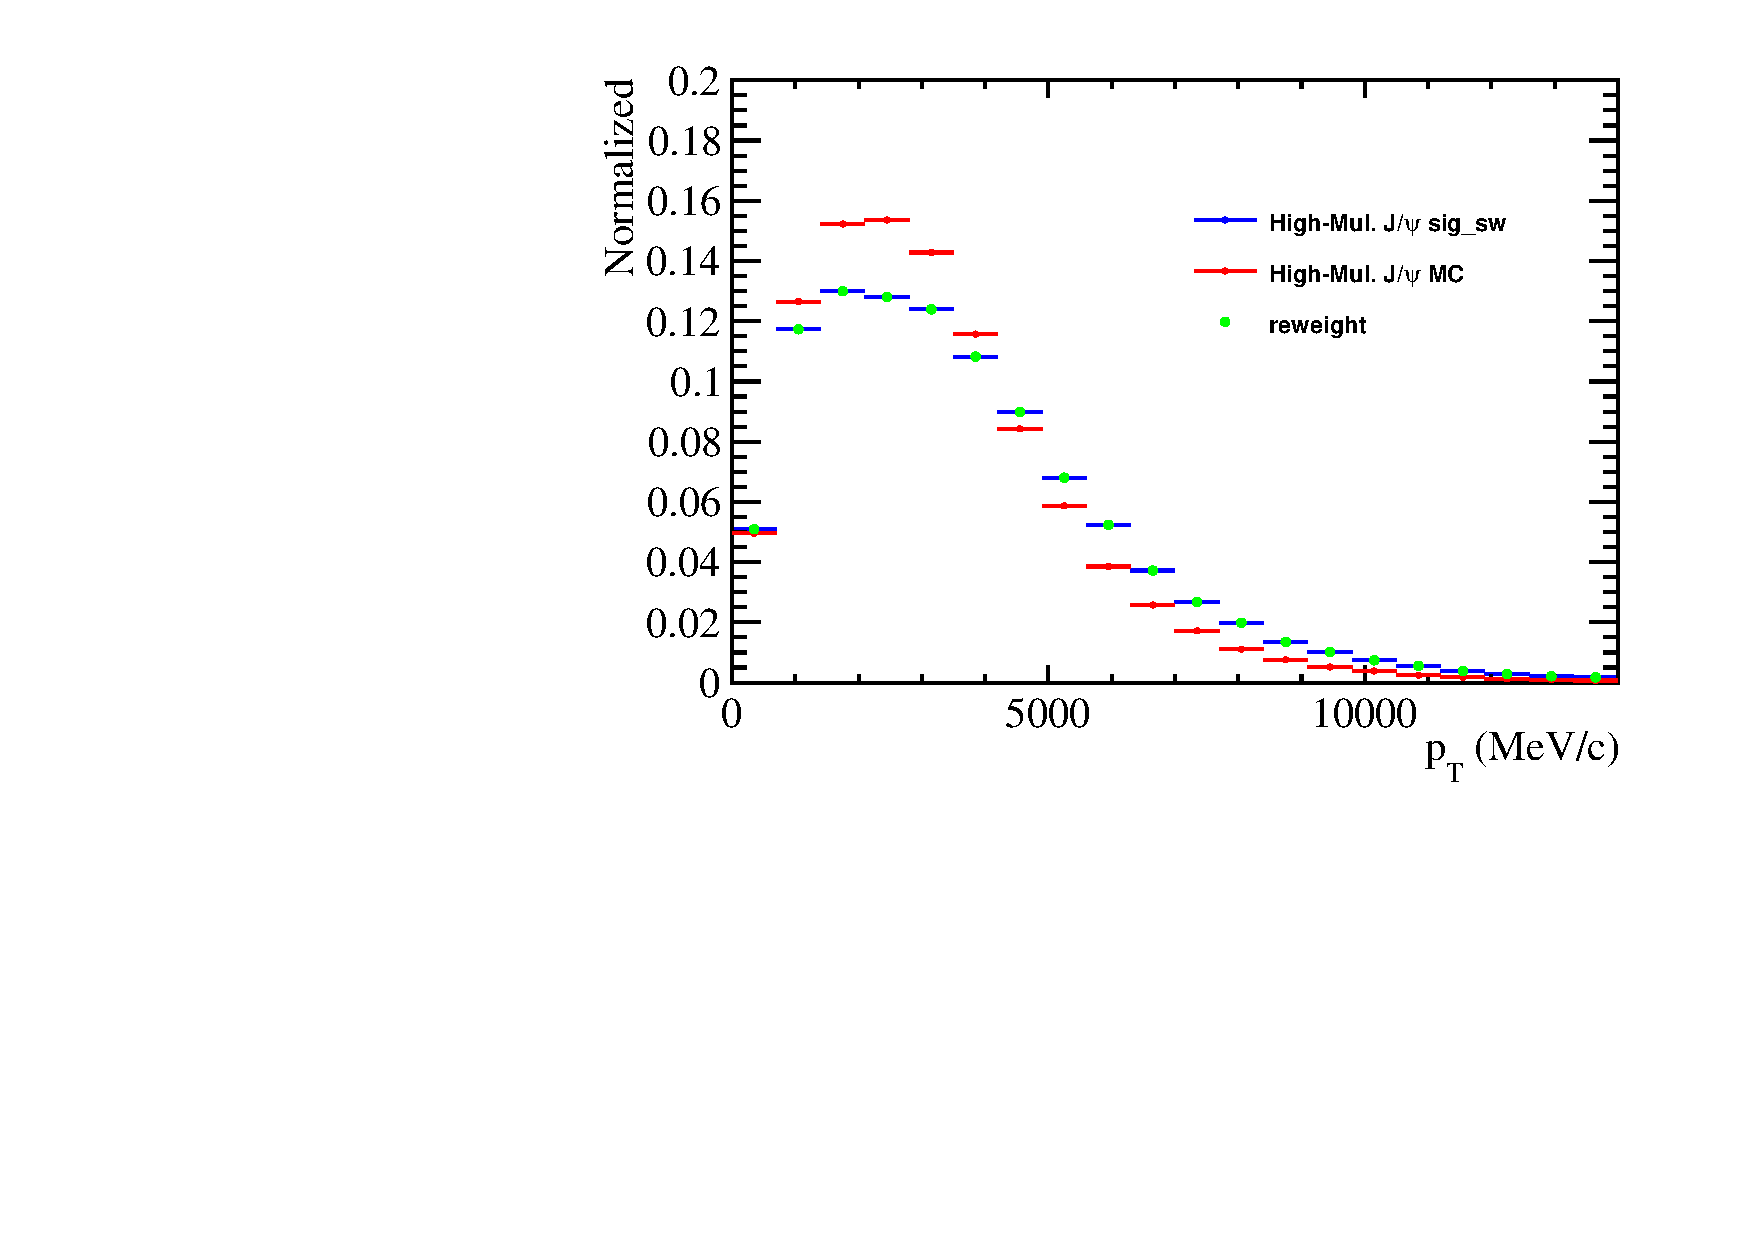
\includegraphics[width=0.37\linewidth]{pdf/pPb/Workdir/Reweight/JpsiHighMulPT.pdf}
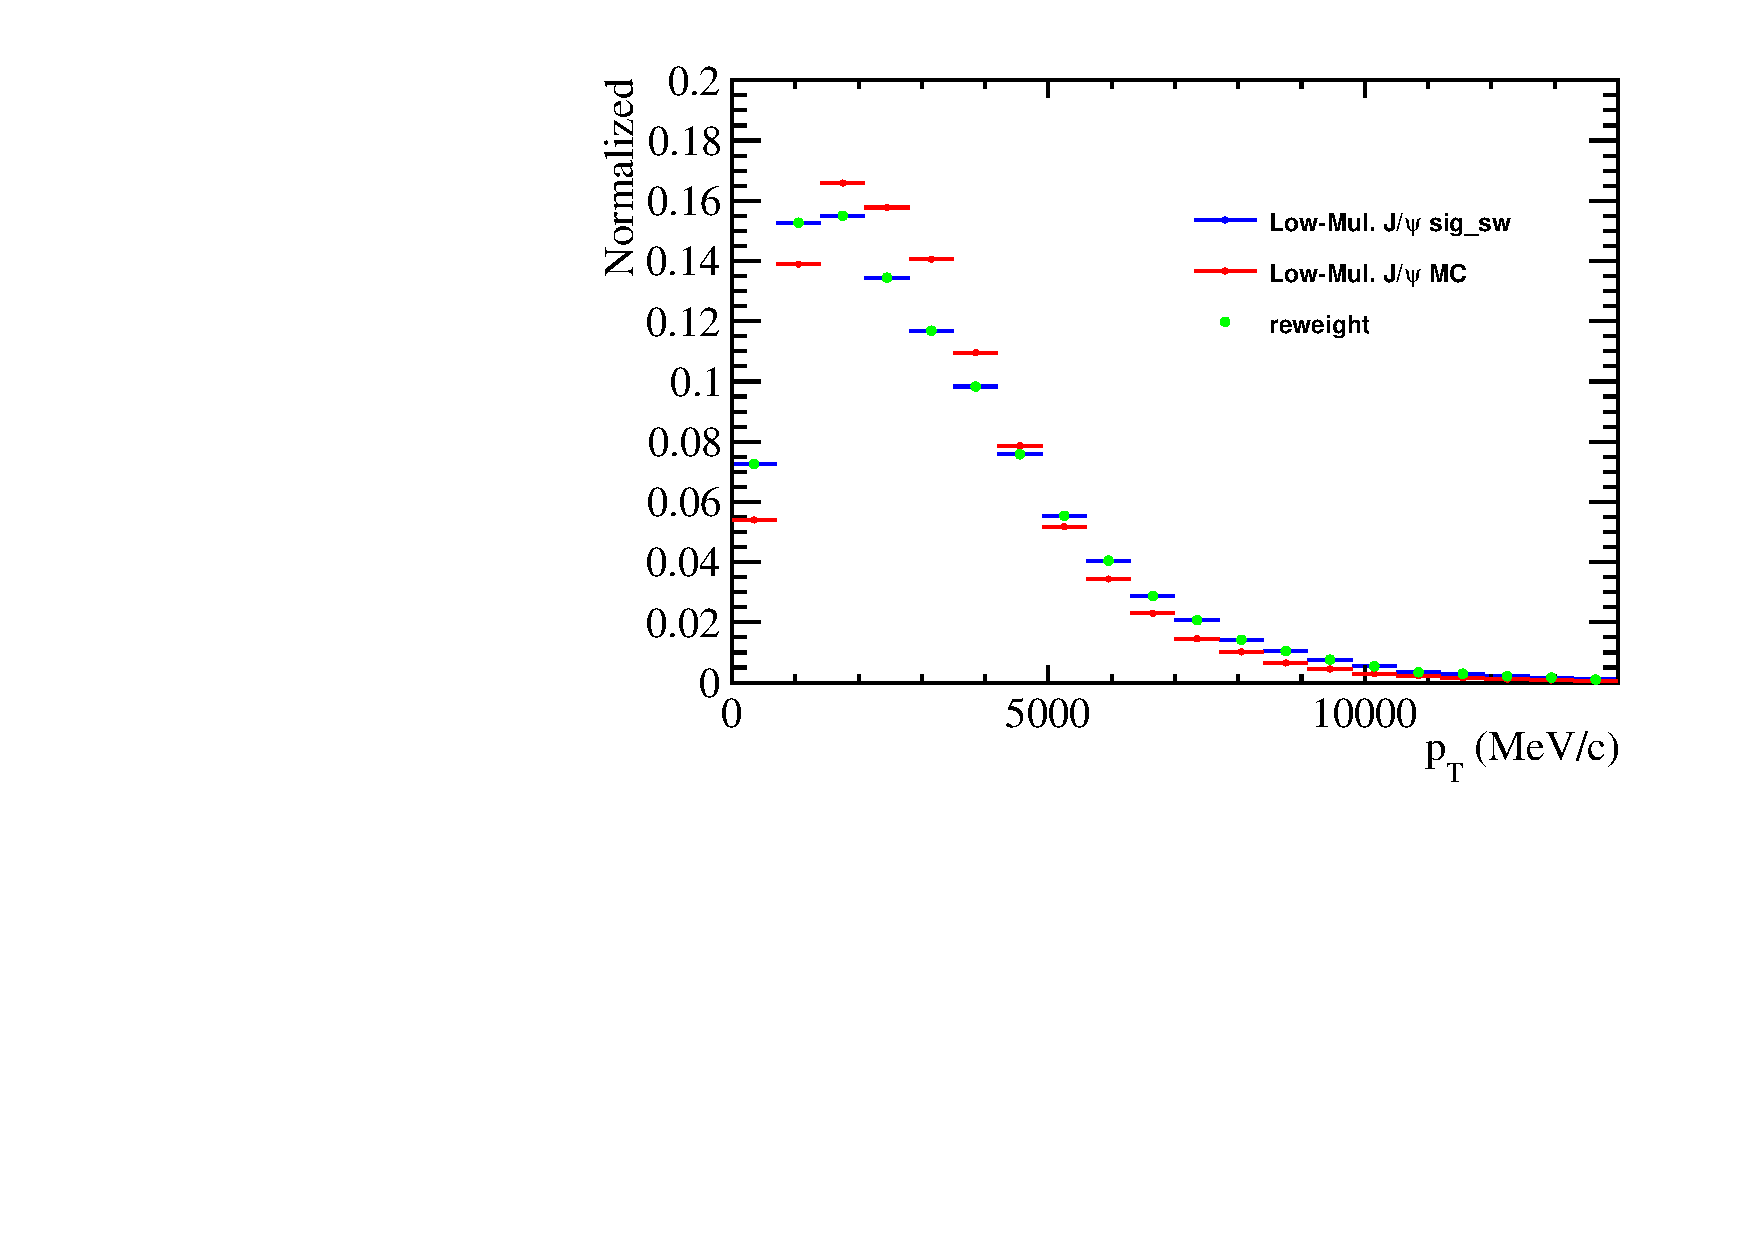
\includegraphics[width=0.37\linewidth]{pdf/pPb/Workdir/Reweight/JpsiLowMulPT.pdf}
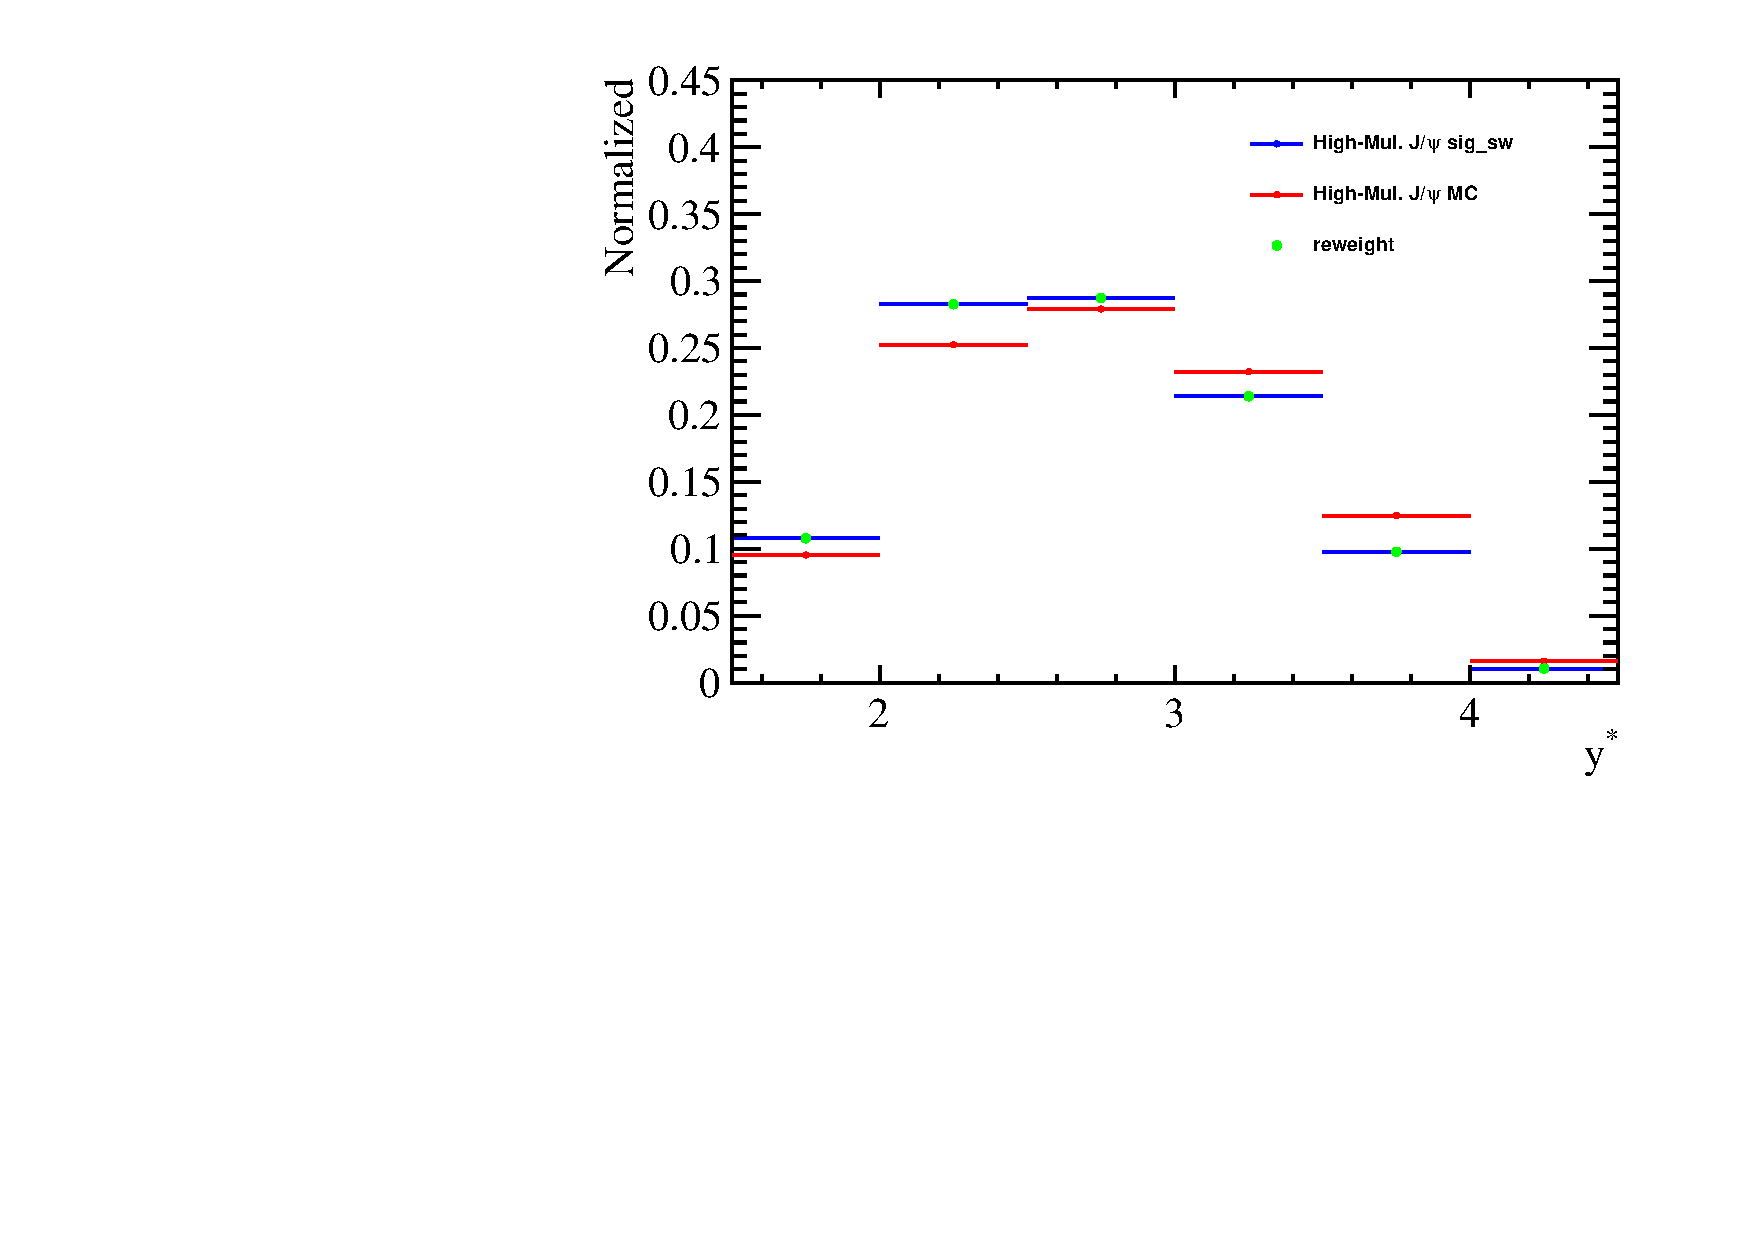
\includegraphics[width=0.37\linewidth]{pdf/pPb/Workdir/Reweight/JpsiHighMulY.pdf}
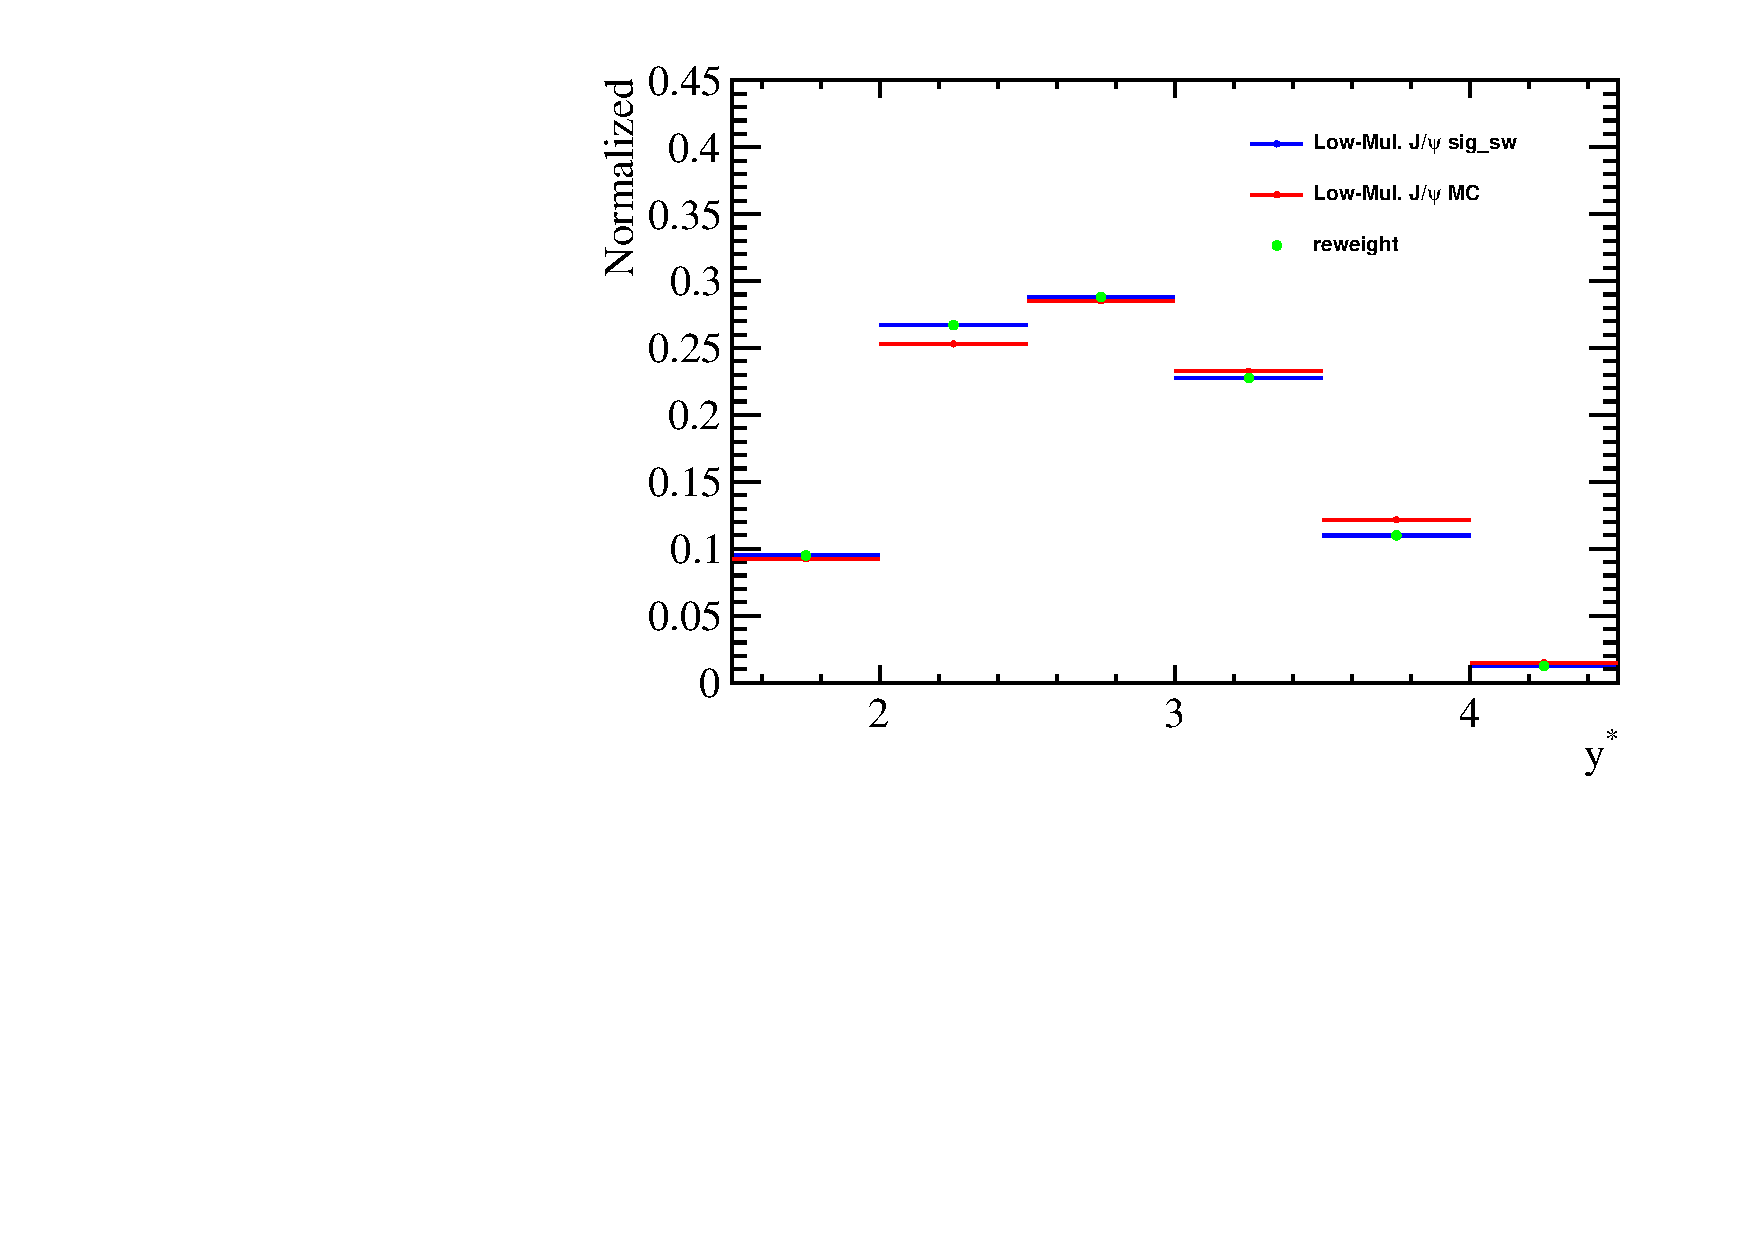
\includegraphics[width=0.37\linewidth]{pdf/pPb/Workdir/Reweight/JpsiLowMulY.pdf}
\end{center}
\caption{
        Re-weight of \pt (first row) and $y^*$ (second row) for high- (left) and low-multiplicity (right) \jpsi samples in $p$Pb configuration.}
\label{PTYReweightJ}
\end{figure}

\begin{figure}[H]
\begin{center}
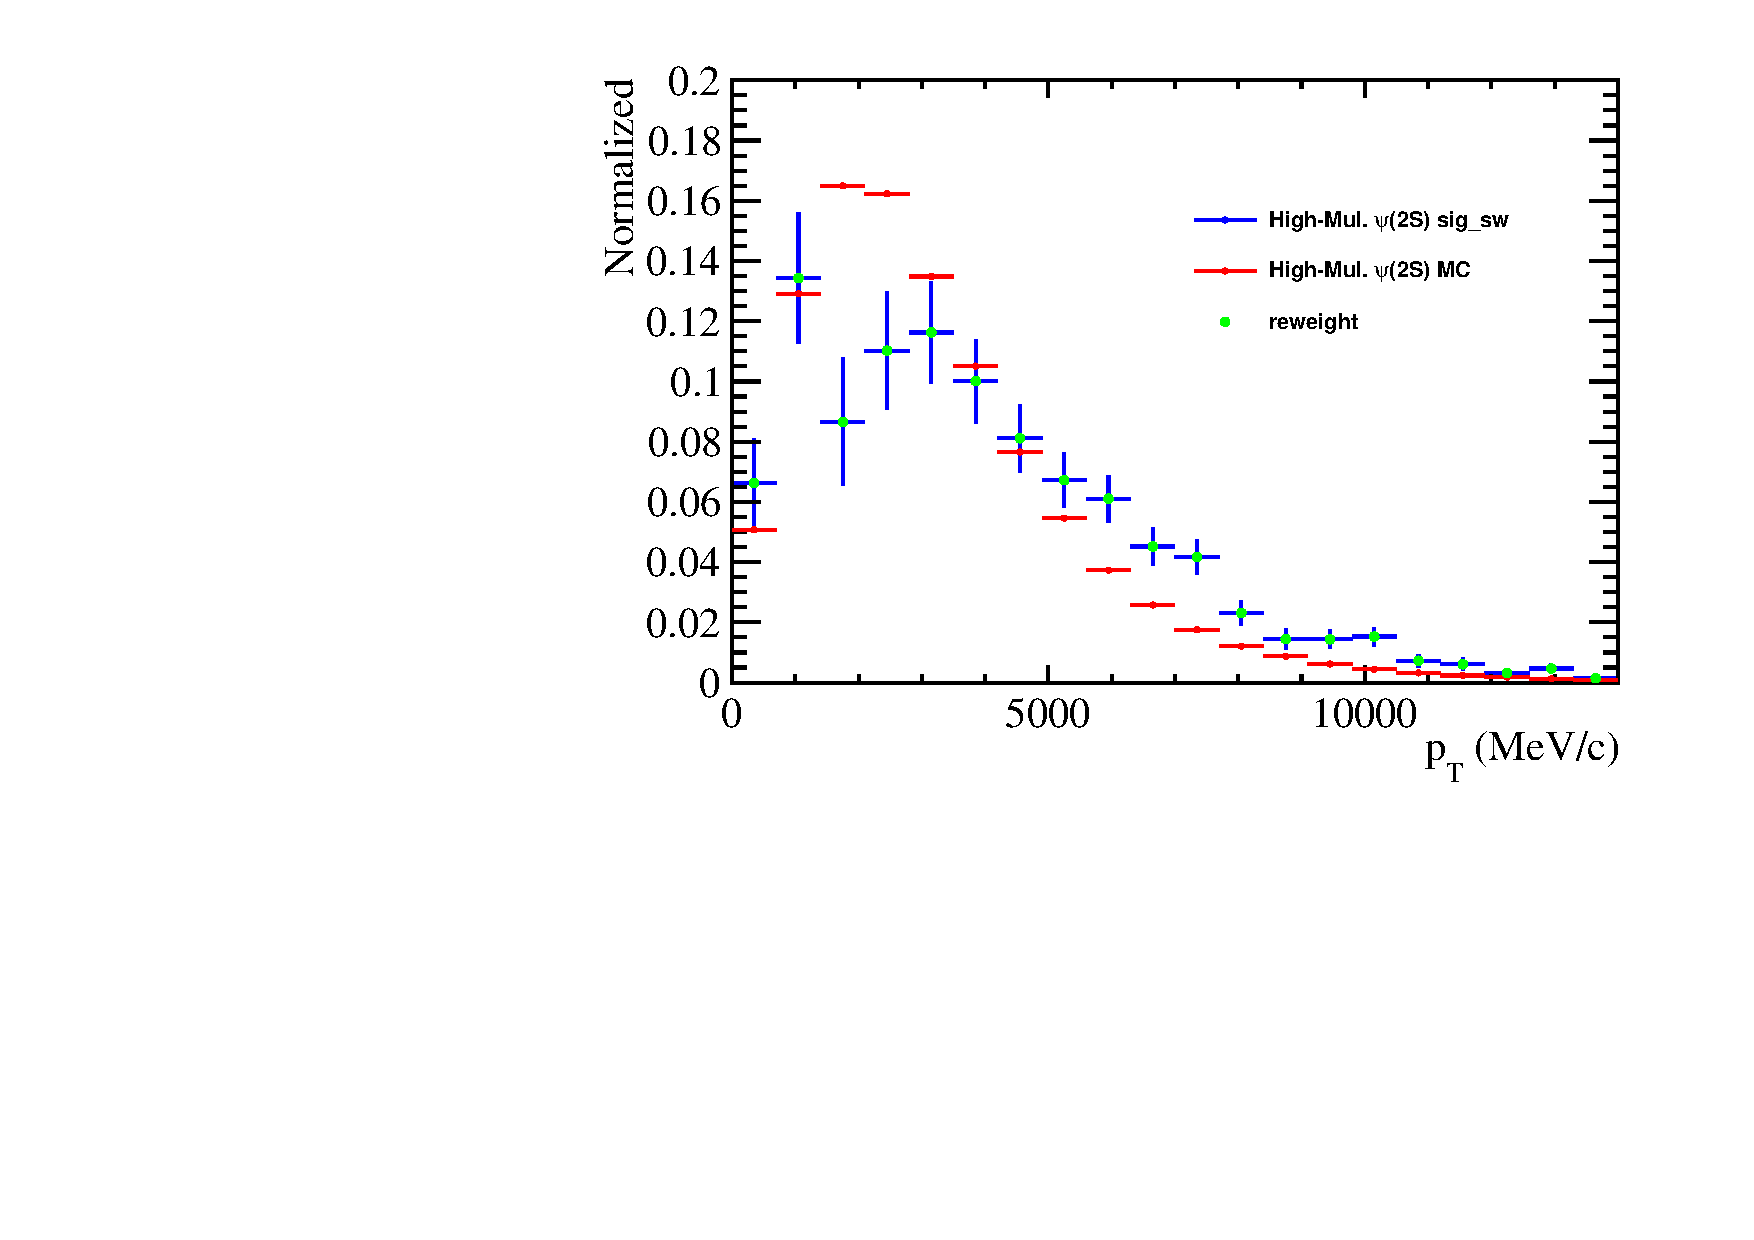
\includegraphics[width=0.37\linewidth]{pdf/pPb/Workdir/Reweight/Psi2SHighMulPT.pdf}
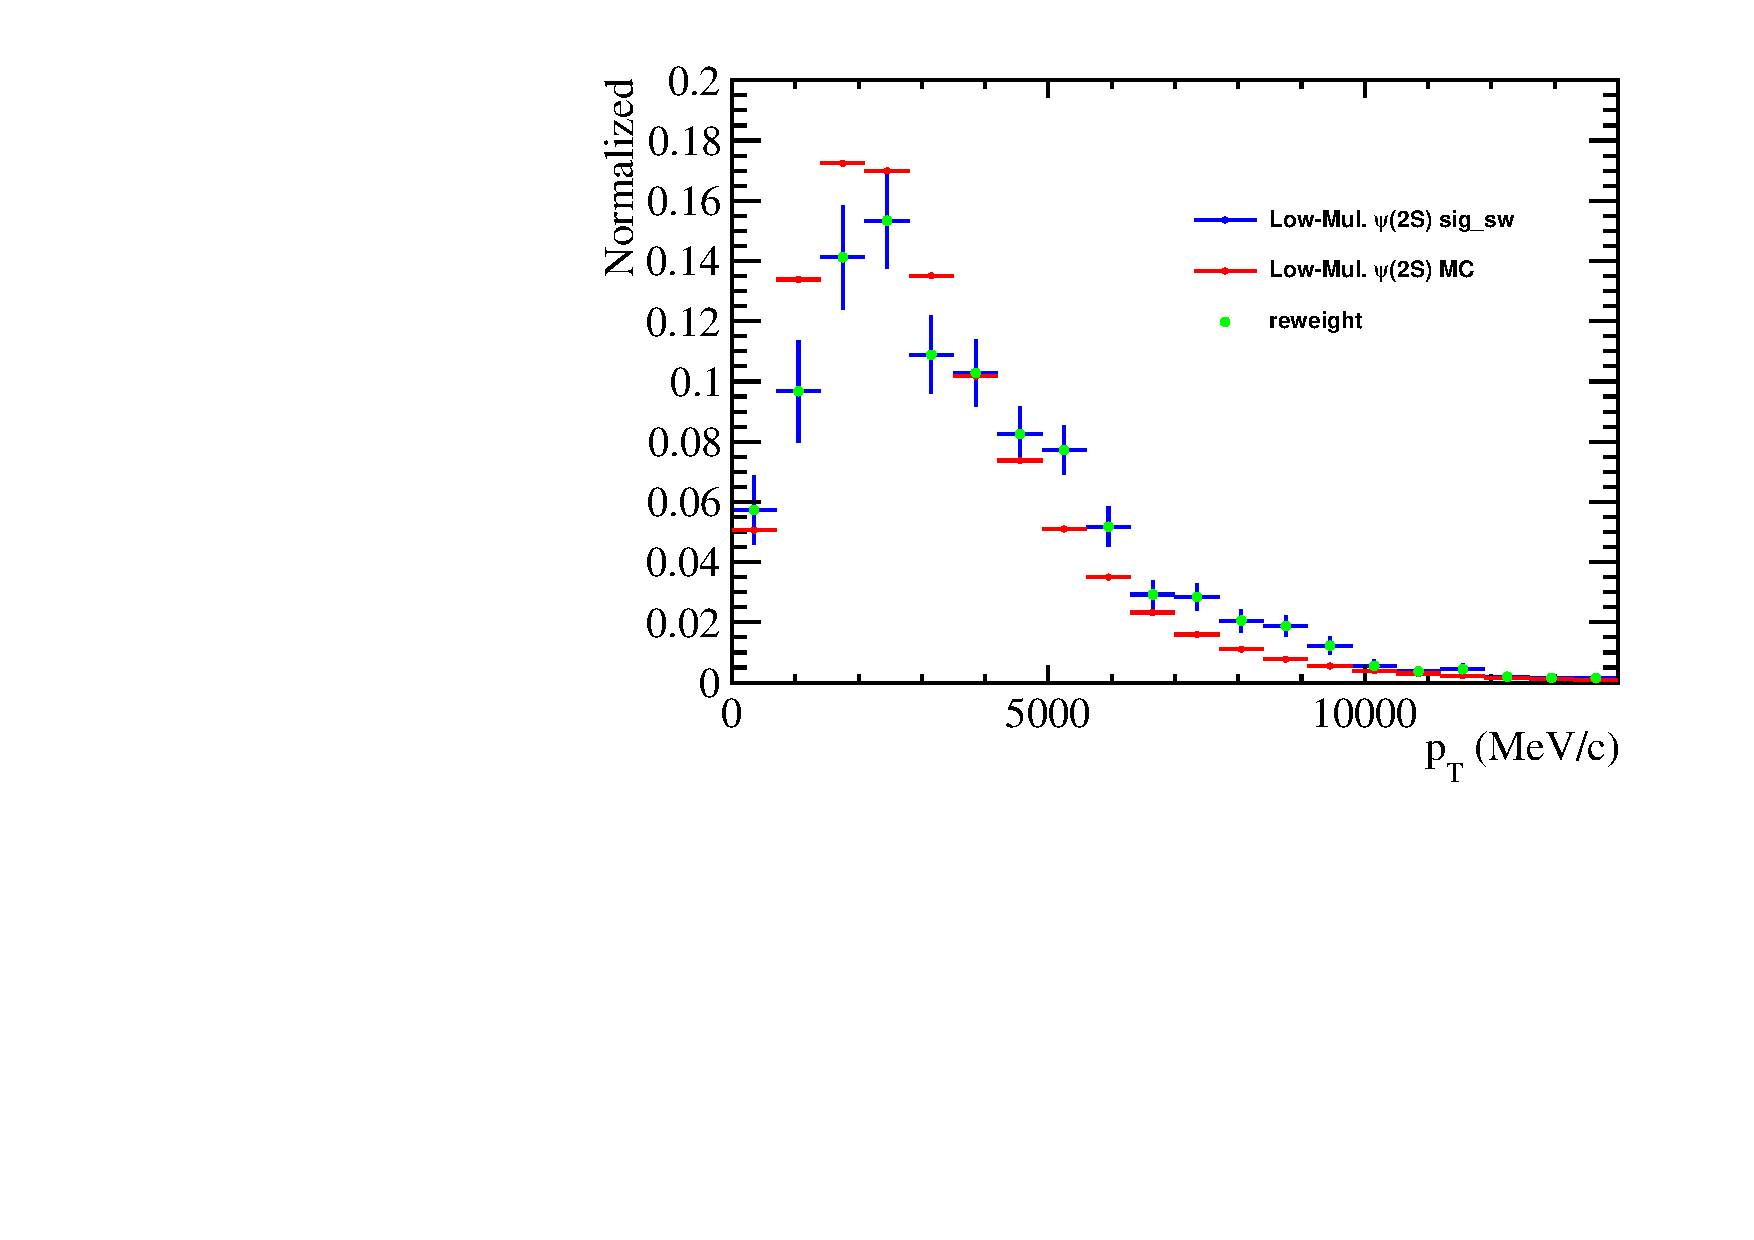
\includegraphics[width=0.37\linewidth]{pdf/pPb/Workdir/Reweight/Psi2SLowMulPT.pdf}
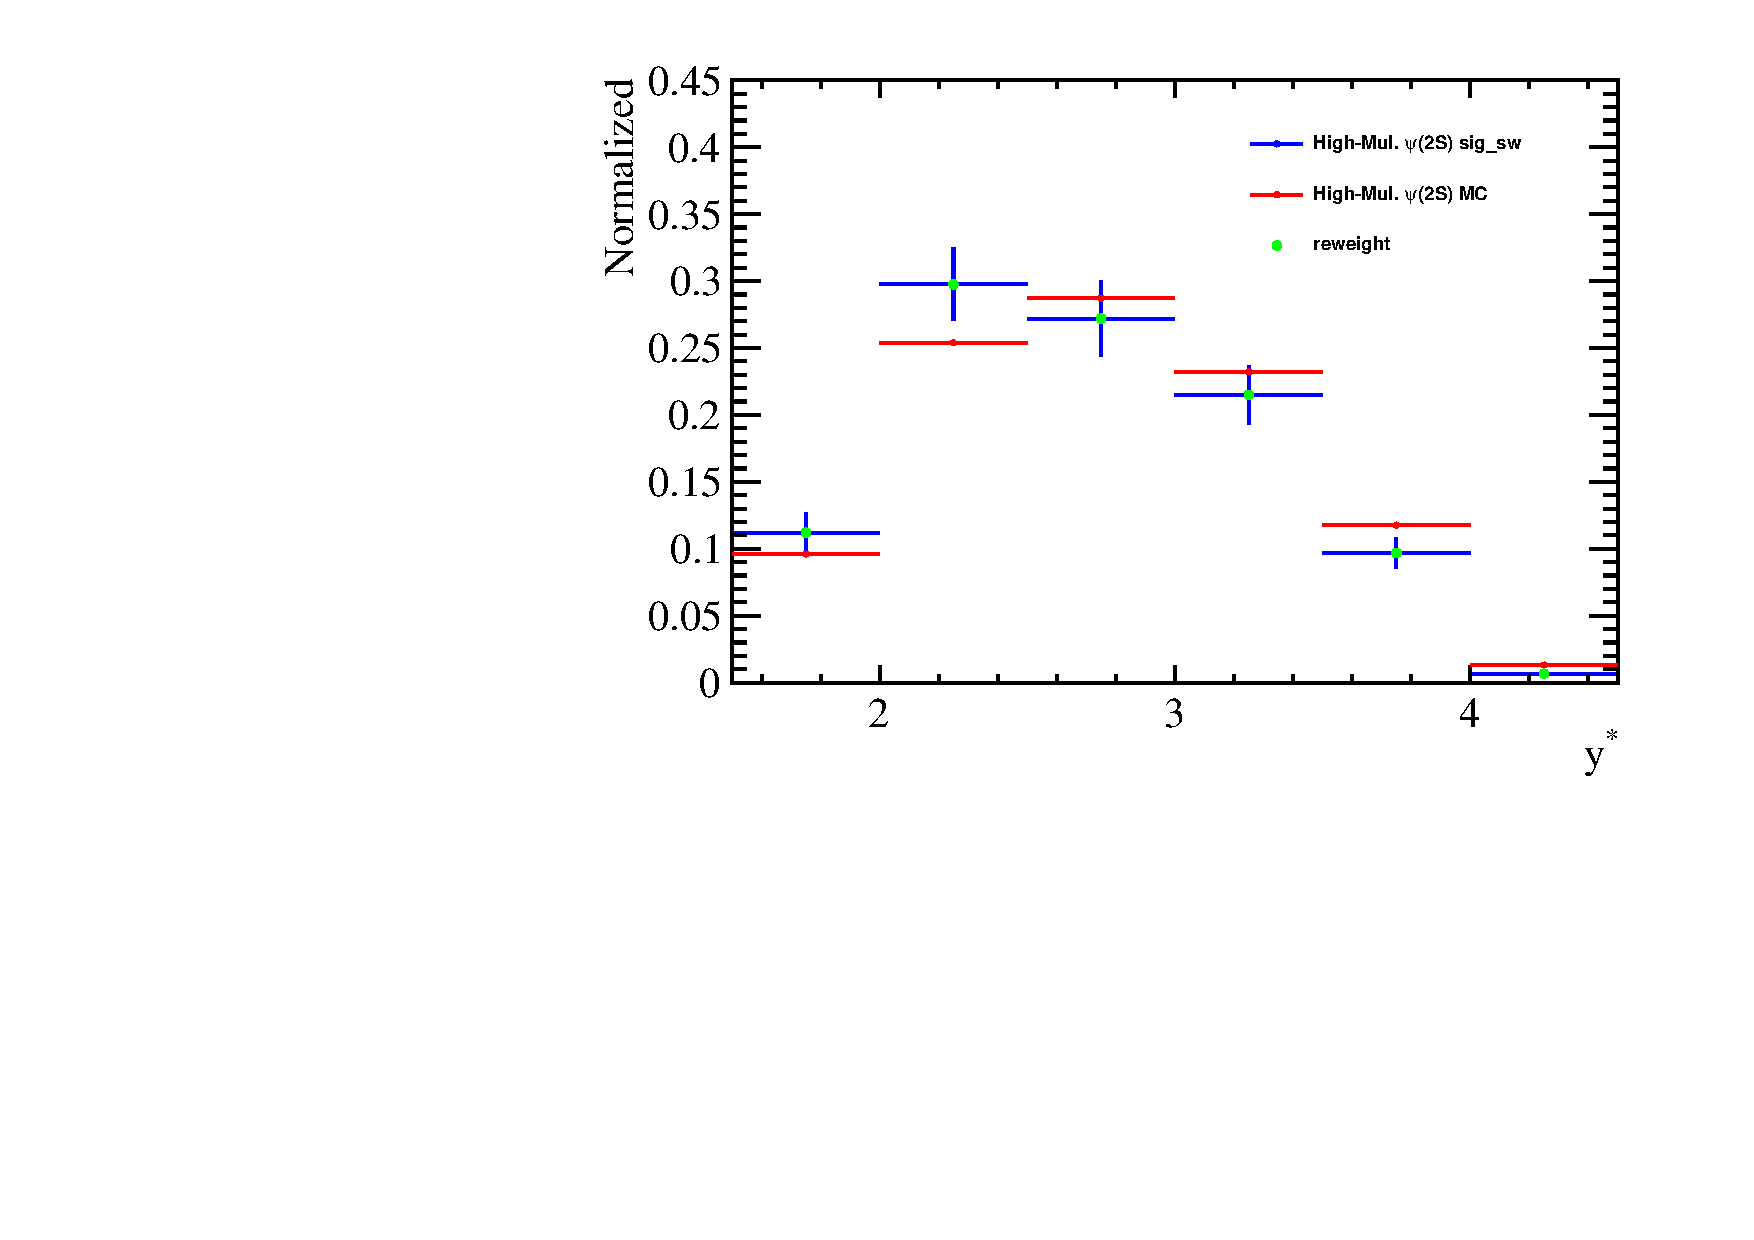
\includegraphics[width=0.37\linewidth]{pdf/pPb/Workdir/Reweight/Psi2SHighMulY.pdf}
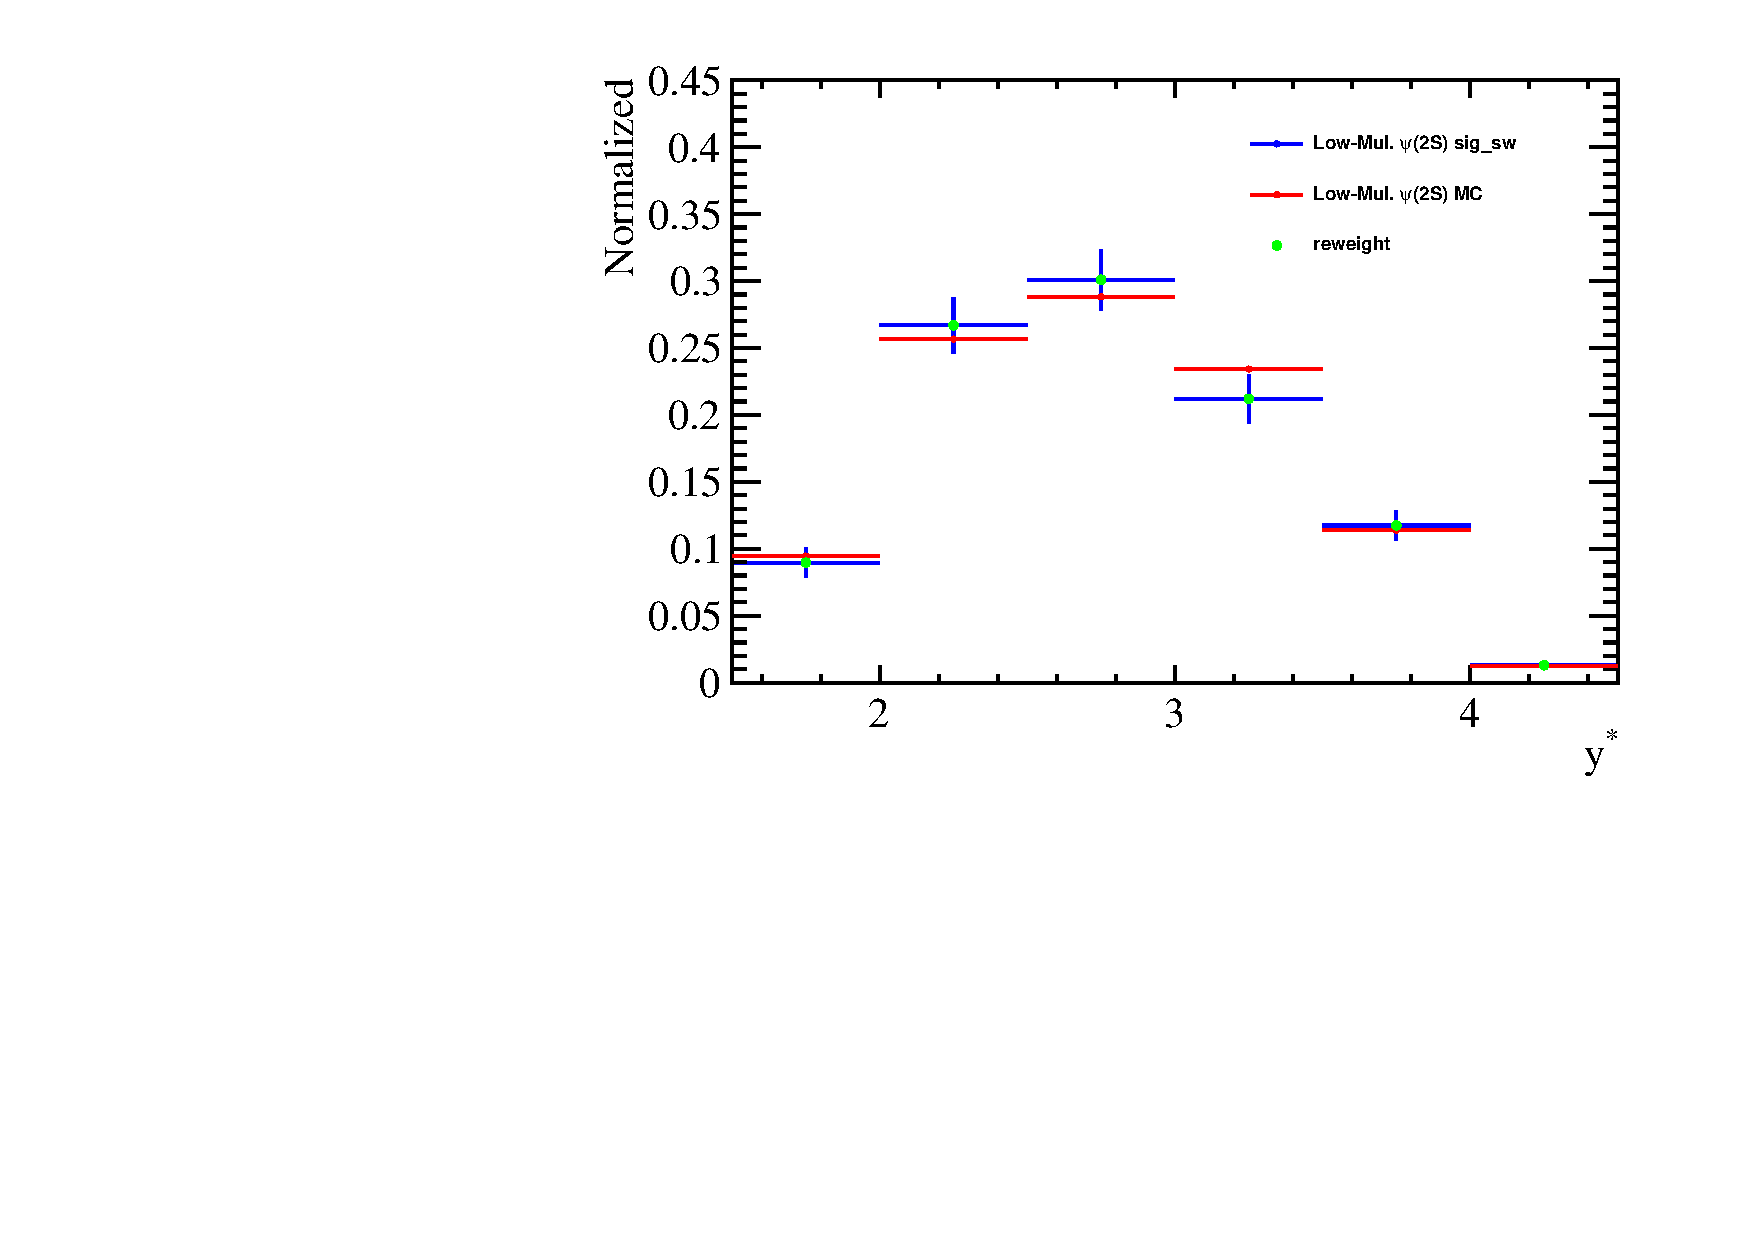
\includegraphics[width=0.37\linewidth]{pdf/pPb/Workdir/Reweight/Psi2SLowMulY.pdf}
\end{center}
\caption{
	Re-weight of \pt (first row) and $y^*$ (second row) for high- (left) and low-multiplicity (right) \psitwos samples in $p$Pb configuration.}
\label{PTYReweightP}
\end{figure}

An example of the \pt reweight table can be find in Fig~\ref{weight}. By assigning each event a corresponding weight according to which \pt bin this event belong to, the \pt distribution for simulated sample can be matched to signal sample, as shown in first plot of Fig~\ref{PTYReweightP}.
\begin{figure}[H]
\begin{center}
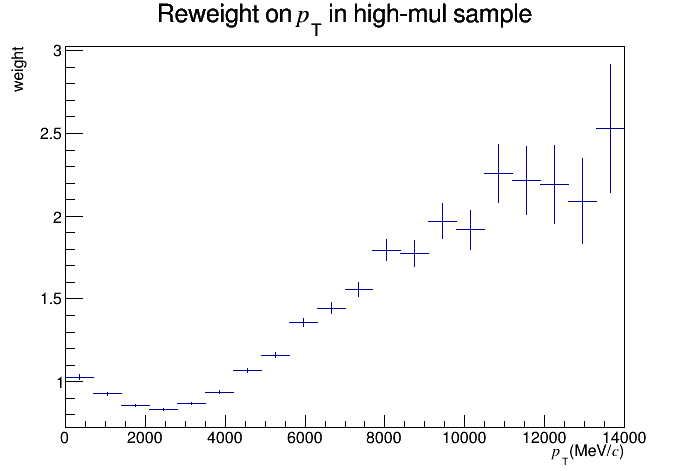
\includegraphics[width=0.49\linewidth]{LHCb-latex-template/latest/latex/figs/w.png}
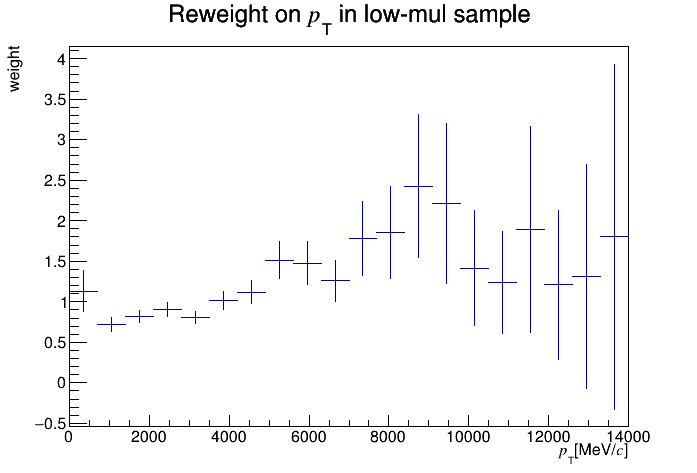
\includegraphics[width=0.49\linewidth]{LHCb-latex-template/latest/latex/figs/wl.png}
\end{center}
\caption{
	Weight in each \pt bin for (left) high-multiplicity and (left) low-multiplicity sample of \jpsi in $p$Pb collisions.}
\label{weight}
\end{figure}

\subsection{Acceptance}
The acceptance efficiency is defined as
\begin{equation}
    \effAcc(\pt,y^*)=\frac{\jpsi(\psitwos) \mathrm{ \ in \  bin \ } (\pt,y^*) \mathrm{ \ with  \ both \ } \mu \mathrm{ \ in \  LHCb \ }}{\jpsi(\psitwos) \mathrm{ \ generated \ in \ bin \ }(\pt,y^*)}
\end{equation}
 It is estimated from generator-level only simulations, using the settings described in Sect~\ref{Data and Monte Carlo samples}. Both $\mu$ in LHCb means here that they have a pseudo-rapidity $\eta$ between 2 and 5, before the magnet. In this analysis we only care about the ratio of acceptance efficiencies $R_{acc}$. When calculating the ratio of acceptance efficiencies, 50 random re-weight tables of \pt (as shown in Fig~\ref{weight}) and $y$ from high- and low-multiplicity samples are generated (100 in total) for both \jpsi and \psitwos. The random table is generated in the following way: Within each bin, a Gaussian random number is generated with mean being the content and sigma being the uncertainty in that bin. Then the 100 tables are introduced as correction to acceptance efficiencies. Then 100 ratios of acceptance efficiencies are calculated. Fit 100 $R_{acc}$ values with a Gaussian function we get the mean value as the ratio of acceptance efficiencies and the sigma be its systematic uncertainty. As an example, the fit result for $R_{acc}$ is shown in Figure~\ref{EffAccRatio}. The value is as follows,
\begin{equation}
	R_{acc}=\frac{\ensuremath{\epsilon_{\mathrm{acc,\jpsi}}}}{\ensuremath{\epsilon_{\mathrm{acc,\psitwos}}}}=0.991\pm 0.012.
\end{equation}
\begin{figure}[H]
\begin{center}
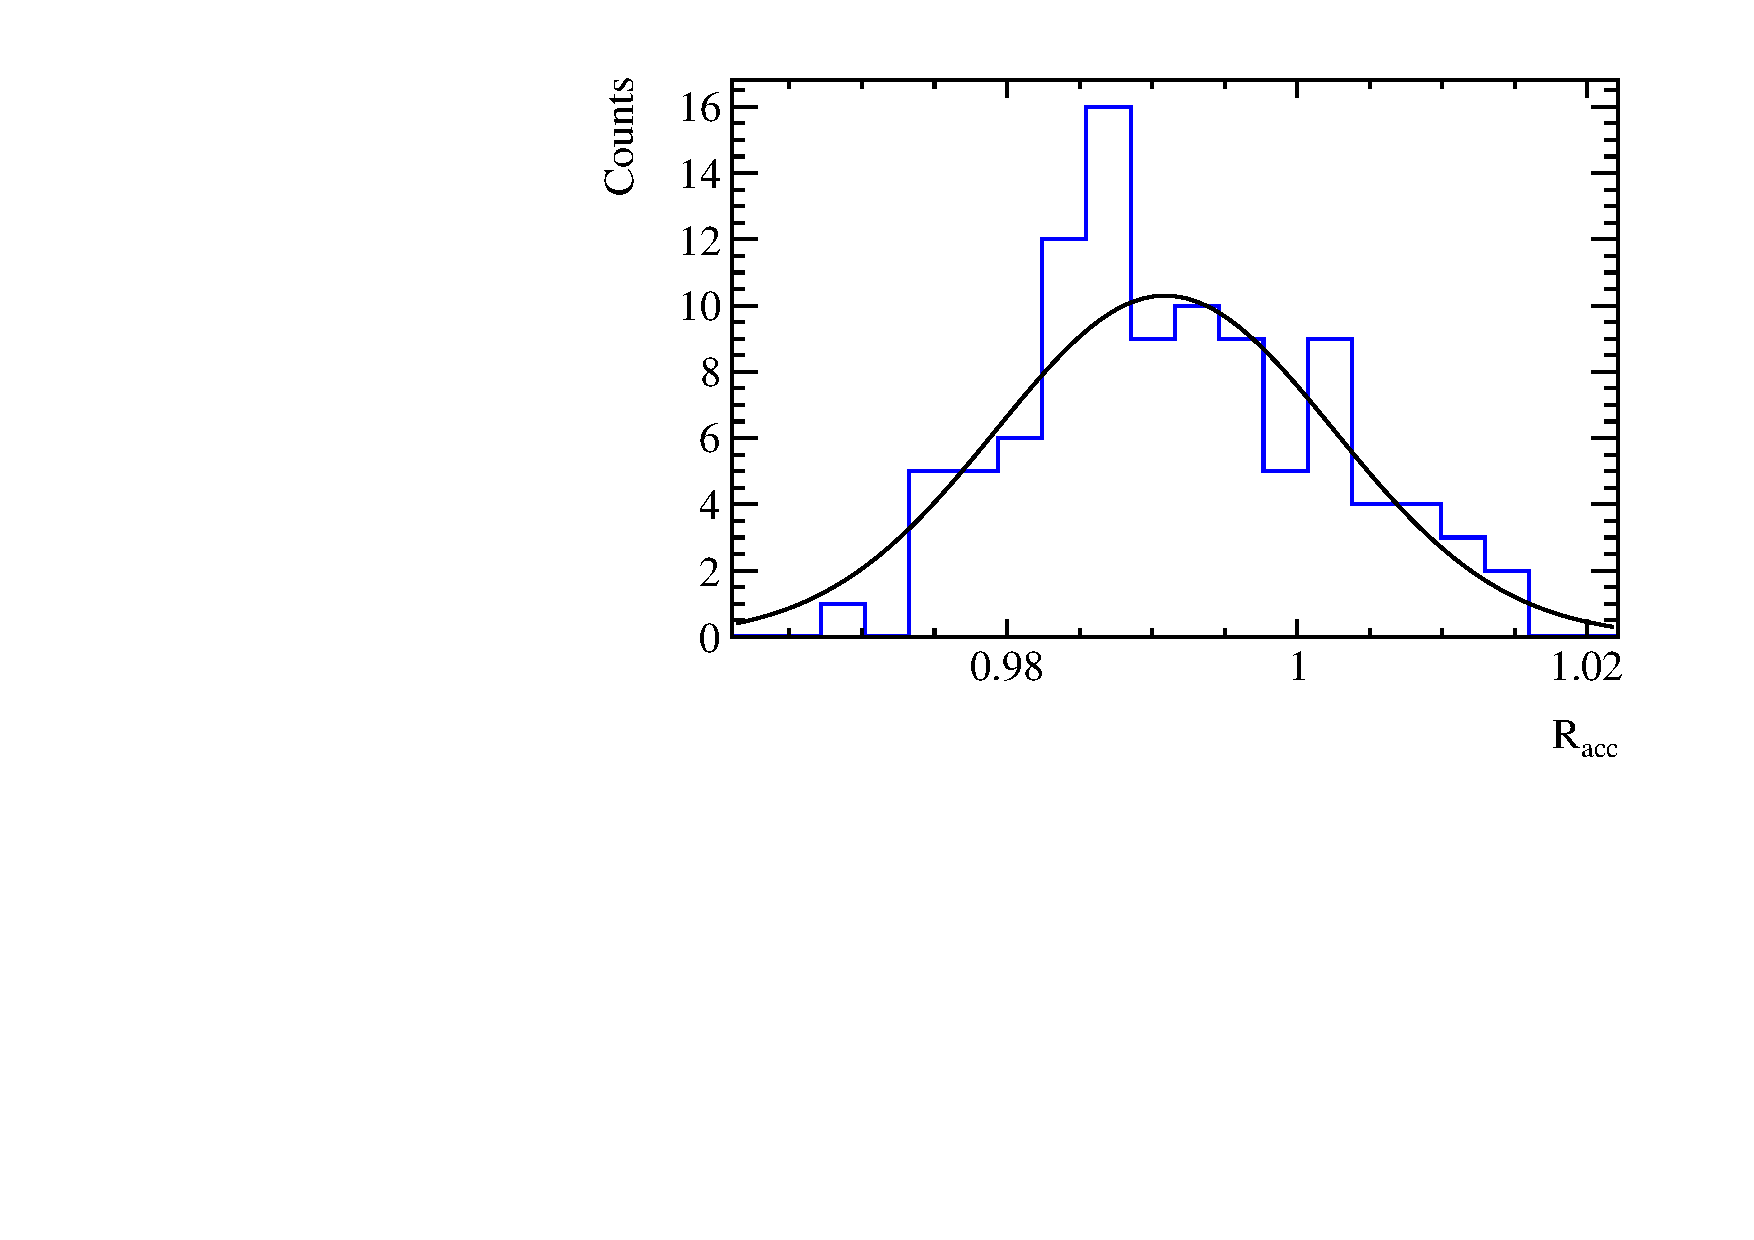
\includegraphics[width=0.5\linewidth]{pdf/pPb/Workdir/Eff_RecselPIDTrigger/Racc.pdf}
\end{center}
\caption{
	Fit Gaussian function on the distribution of $R_{acc}$ in $p$Pb collisions from 100 trials with global cuts for $N_{\rm tracks}^{\rm PV}$ as multiplicity variable.}
\label{EffAccRatio}
\end{figure}


 \subsection{Reconstruction and selection efficiency}
 The reconstruction and selection efficiency is defined as the fraction of \jpsi (\psitwos) in the acceptance, where both muons are reconstructed as long tracks and then pass the offline selections,
 \begin{equation}
    \effReco(\pt,y^*)=\frac{\jpsi(\psitwos) \mathrm{ \ in \  bin \ } (\pt,y^*) \mathrm{ \ with  \ both \ } \mu \mathrm{ \ reconstructed \ and \ selected}}{\jpsi(\psitwos) \mathrm{ \ in \  bin \ } (\pt,y^*) \mathrm{ \ with  \ both \ } \mu \mathrm{ \ in \  LHCb \ }}.
\end{equation}
%The tracking efficiency is computed using the simulation samples, and this efficiency is corrected using the reconstruction efficiency per-track estimated in data. The long method with tag-probe strategy for tracking efficiency calibration is implemented. In this method, a probe track is reconstructed only with hits in the TT and MUON stations. This probe muon track is combined with a standard long muon track to form a \jpsi candidate, and these candidates build a “pre-matched” sample. This standard long track has the same reconstruction algorithm as the signal tracks in our analysis, so they have the same tracking efficiency when they are in the same phase space. 
An additional standard long track, identified as a muon and with the same charge as the probe track, is combined with the \jpsi in the ”pre-matched” sample to form a good vertex. If this third track shares with the probe track more than $40\%$ of the hits in both the TT and MUON stations, the probe track is referred to as “matched”. The \jpsi candidates in the ”pre-match” sample that have the probe track matched, form the ”matched” sample. 
The tracking efficiency is computed as the matching efficiency, which is the fraction of probe tracks that match standard long tracks. The number of signal probe tracks and those matched to long tracks are estimated from the number of \jpsi signal candidates, measured by fitting to the $\mu^+\mu^-$ invariant mass distribution in the ”pre-matched” sample and the ”matched” sample, respectively. The reconstruction of the probe tracks, of the \jpsi candidates and the implementation of the matching are done at the trigger (HLT) level, available in both pp and proton-lead data. The relevant trigger lines are called $\textbf{Hlt2TrackEffDiMuonMuonTT(Minus|Plus)^*}$ (which selects the “pre-matched” samples), where Plus (Minus) means that the $\mu^+(\mu^-)$ is the probe track. These calibration events are processed via the TurboCalib stream. Due to higher multiplicity in proton-lead data, especially in the backward configuration, additional offline selections are applied to the \jpsi candidates out of TurboCalib stream. The tag track of the \jpsi candidates is required to have a good muon-pion separation with $PID(\mu)$ > 3, and the probe track is required to have a better fit quality with $Prob(\chi_{trk}^2) > 0.2$. The effect of these extra selections is studied with the proton-lead forward data sample ($p$Pb), where a better signal purity is obtained. 
Simulated \jpsi samples are produced with the same trigger processing as data for the calibration. The reconstruction software is identical to those used to reconstruct the simulated signals used in the analysis. 
The signal extraction fits to the mass distributions are implemented in bins of $\eta$ and $p$ of the probe tracks, allowing to determine the track reconstruction efficiency in the same bins. The bin boundaries are 1.9, 3.2 and 5.0 for $\eta$ and 6, 10, 20, 40, 100 and 500 $\gevc$ for $p$. No binning in detector occupancy is implemented due to limited statistics. However, since for both data and simulation, the occupancy distribution in the analysis samples and the calibration samples are consistent with each other,  the binning in detector occupancy is not necessary. 
The $\mu^+$ and $\mu^-$ probe tracks are fit separately. Thus for each kinematic bins, there are eight fits: $\mu^+$ or $\mu^-$ as the probe track; in the ”pre-matched” or ”matched” sample; for $p$Pb or Pb$p$. For the fits, the same signal shape is used for bins of the same $(p, \eta)$ interval: a Gaussian function plus a Crystal Ball function. The background is described by an exponential function. 
The procedure performed on data is applied identically to the $p$Pb and Pb$p$ simulation calibration samples. The tracking efficiencies for $\mu^+$ and $\mu^-$ are averaged, as for the cross-section measurements charge conjugated states are added together.
Finally, we calculate the ratio of single track reconstructions efficiencies between data and simulation. The results are given in Figure~{TrackTable}. The corresponding uncertainty for each value is also shown. The ratio reconstruction and selection efficiency is then computed from the full simulation, and correcting the efficiency using the per-track efficiency ratios detailed above.
Then the reconstruction efficiency is further corrected using the data-over-simulation single tracking efficiency ratio. The ratio of tracking efficiencies for a single track in data and simulation determined with the Long Tag-Probe method is shown in Figure~\ref{TrackTable} which was given by the tracking group~\cite{Trackweb}. For a given event the correction factor is determined by multiplying the efficiency ratios for each of the tracks in the final state.
\begin{figure}[!tbp]
\begin{center}
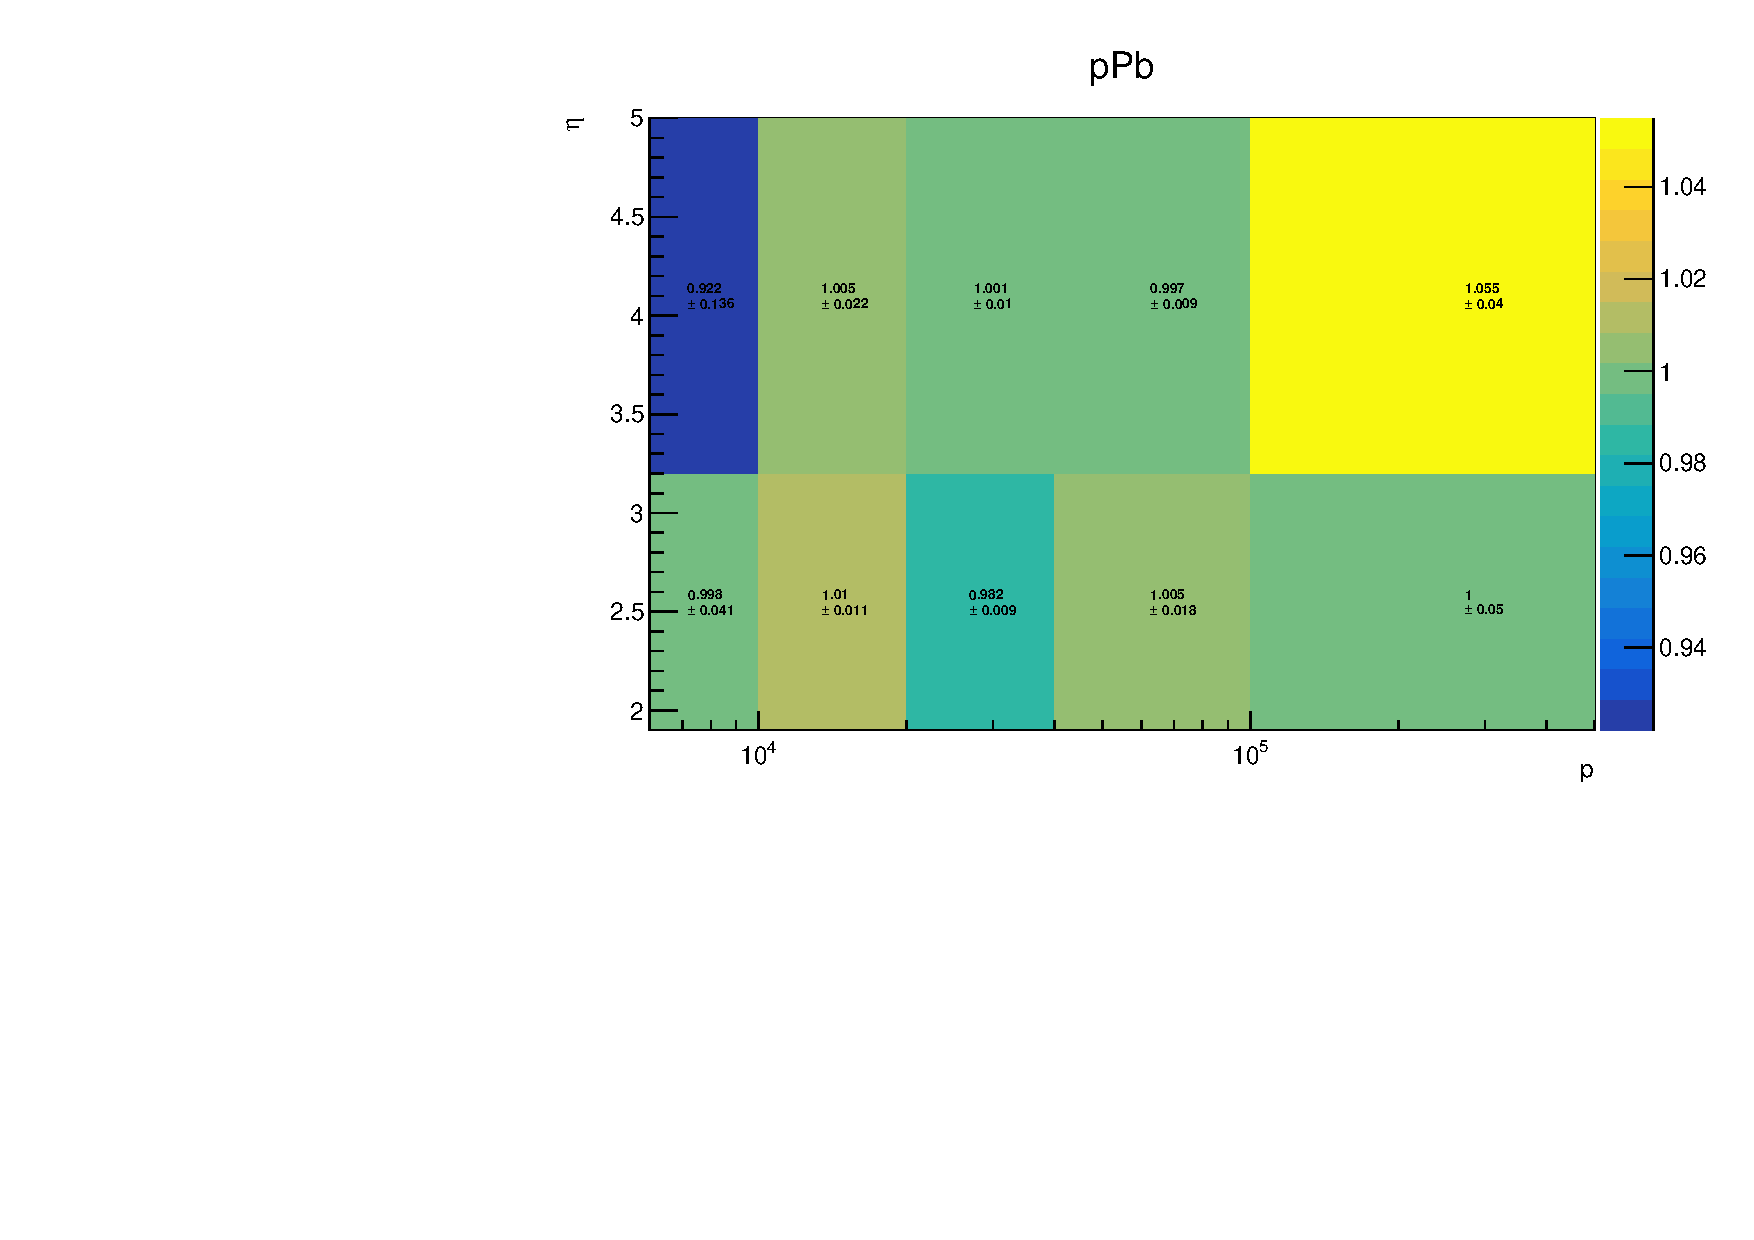
\includegraphics[width=0.49\linewidth]{pdf/pPb/Workdir/TrackCalib/pPb.pdf}
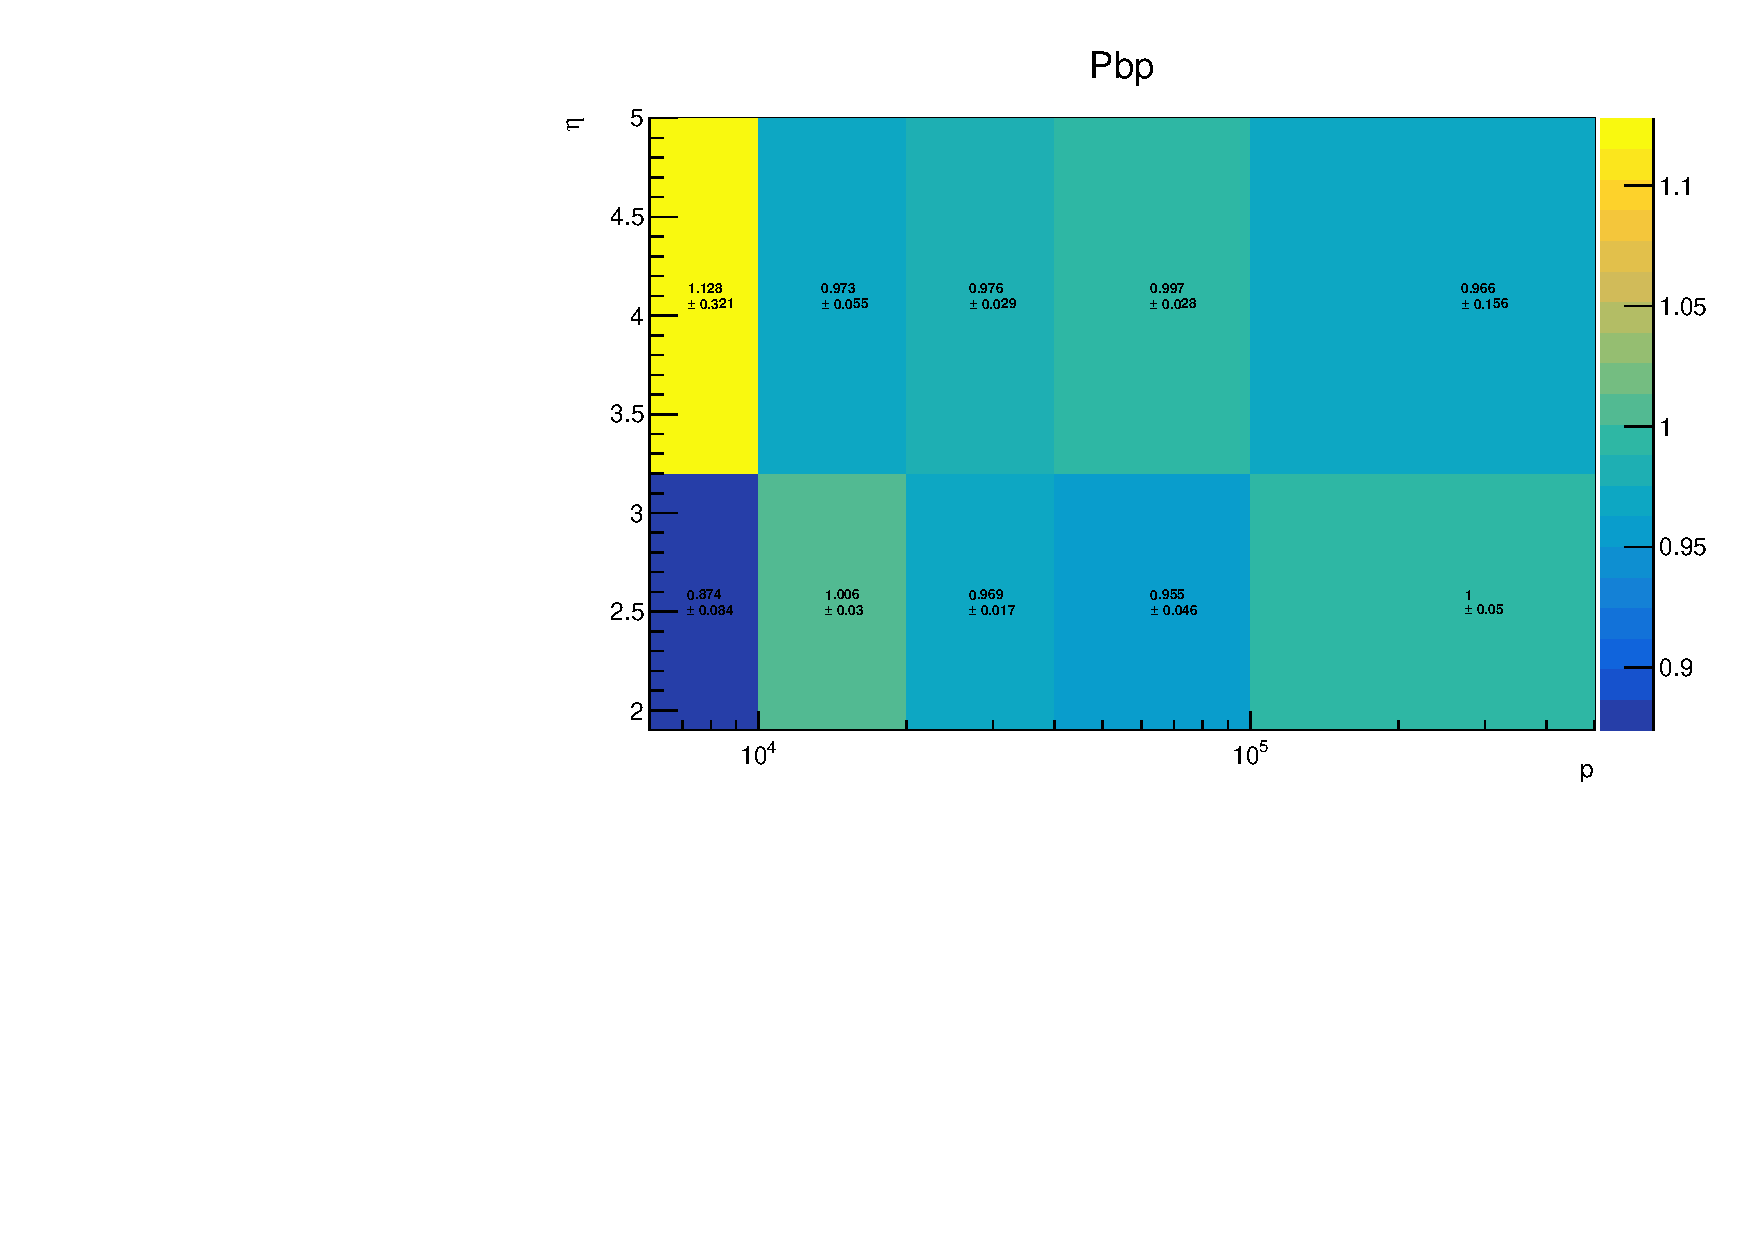
\includegraphics[width=0.49\linewidth]{pdf/pPb/Workdir/TrackCalib/Pbp.pdf}
\end{center}
	\caption{Ratio between data and $p$Pb (left) and Pb$p$ simulation of per-track tracking efficiency in bins of the track $\eta$ and $p$.
    }
\label{TrackTable}
\end{figure}

From Eq.~\ref{EffRatio} we can see that, we calculate the ratio of all the efficiencies $R_{eff}$ (except for acceptance efficiencies) as a whole part, since they are all calculated with full-simulation Monte Carlo sample. Another reason is, when calculating \effReco, \effID and \effTrigger, 500 random tables of \pt and $y^*$ from high- and low-multiplicity samples are generated (1000 in total) for both \jpsi and \psitwos in $p$Pb and Pb$p$ configurations and introduced to correct the imperfection on simulation to data. For a certain trial, the re-weight on \pt (or $y^*$) may under- or over-estimate  \effReco, \effID and \effTrigger simultaneously, it is hard to determine the dependence between these efficiencies. So a good way is to calculate them as a whole, each time a certain random re-weight table is introduced. The definition of $R_{eff}$ is in Eq.~\ref{Reff}.
\begin{equation}
R_{eff}\bigg|_{Mult. \ bin} = 
\frac{\ensuremath{\epsilon_{\mathrm{Reco\&Sel,\jpsi}}}\cdot\ensuremath{\epsilon_{\mathrm{MuonID,\jpsi}}}\cdot\ensuremath{\epsilon_{\mathrm{Trigger,\jpsi}}}}{\ensuremath{\epsilon_{\mathrm{Reco\&Sel,\psitwos}}}\cdot\ensuremath{\epsilon_{\mathrm{MuonID,\psitwos}}}\cdot\ensuremath{\epsilon_{\mathrm{Trigger,\psitwos}}}}\bigg|_{Mult. \ bin}.
\label{Reff}
\end{equation}
Similarly, 1000 random tables for data-over-simulation single tracking efficiency ratio are generated and introduced into the 1000 trials, and 1000 random tables for efficiency table obtained from PIDCalib package~\cite{Archilli:2013npa} are introduced in each trial as well to calculate PID efficiencies, and hence, $R_{eff}$, as stated in the following part. So we will give an overall estimation (values and uncertainties) for $R_{eff}$ after introduced \effID and \effTrigger.

\subsection{PID efficiency}
The PID efficiency is defined as 
\begin{equation}
    \effID(\pt,y^*)=\frac{\jpsi(\psitwos) \mathrm{ \ satisfying \ PID \ selection \ in \ bin \ }(\pt,y^*)}{\jpsi(\psitwos)\mathbf{ \ selected \ in \ bin \ }(\pt,y^*)}.
\end{equation}
The PID efficiency for muons is taken from data using calibration tables (PIDCalib tables) obtained from control samples, namely \jpsi candidates. These calibration tables give the efficiency of the PID selections as a function of the pseudo-rapidity, of the total momentum of the muon tracks and of the track multiplicity of the event estimated from the number of hits in the SPD. They are available for the $pp$, $p$Pb and Pb$p$ data taking. 
The muon ID efficiency in each $(\pt,y^*)$ bin is then calculated by averaging the muon ID efficiency of each candidate in the bin, which is the product of the muon ID efficiencies of the two muons from the efficiency table, according to their $(p, \eta, nSPDhits)$ values. As mentioned above, calculation on \effID for \jpsi and \psitwos is only a component of calculation of $R_{eff}$. So 1000 random tables are generated from the PIDCalib efficiency table and introduced to each trial of $R_{eff}$ calculations.

\subsection{Trigger efficiency}
The trigger efficiency is defined as follows
\begin{equation}
    \effTrigger(\pt,y^*)=\frac{\jpsi(\psitwos)\mathrm{ \ TOS of \ L0 \ and \ HLT1 \ in \ bin \ }(\pt,y^*)}{\jpsi(\psitwos)\mathbf{ \ selected \ in \ bin \ }(\pt,y^*)},
\end{equation}
where the selection includes the PID requirements. The efficiencies are computed with the simulated samples, with the PID cut 
requirements to both the numerator and denominator. Note that since the analysis is done on the TURBO candidates, the efficiency of the HLT2 is included in the reconstruction, PID and selection efficiencies. When calculating the trigger efficiencies for \jpsi and \psitwos, same random tables generated from re-weight tables of \pt and $y^*$ are used as that used in \effReco and \effID above for each one of the 1000 trials.

\subsection{Total efficiency}
Finally, the 1000 ratios of all the efficiencies except geometric acceptance $R_{eff}$'s are fitted with a Gaussian function. Hence, we can calculate the ratio of total efficiencies $R_{tot}=R_{acc}\times R_{eff}$ with the following systematic uncertainties considered,
\begin{itemize}
    \item re-weight of \pt distribution from high- and low-multiplicity samples,
    \item re-weight of $y^*$ distribution from high- and low-multiplicity samples,
    \item uncertainties due to the limit calibration sample size in PIDCalib efficiency table,
    \item uncertainties of data-over-simulation ratio of per tracking efficiency.
\end{itemize}
Systematic uncertainties from other sources will be discussed in Sec~\ref{Systematic uncertainty}. As an example, the fit results for $R_{eff}$ in different $N_{\rm tracks}^{\rm PV}$ classes for $p$Pb configuration are shown in Figure~\ref{ReffPlots}. The corresponding values of $R_{eff}$ with uncertainties mentioned above are summarized in Table~\ref{ReffTable_PVNTRACKS_pPb}. The summary tables for other multiplicity variables and configurations can be found in appendix.
\begin{figure}[!tpb]
\begin{center}
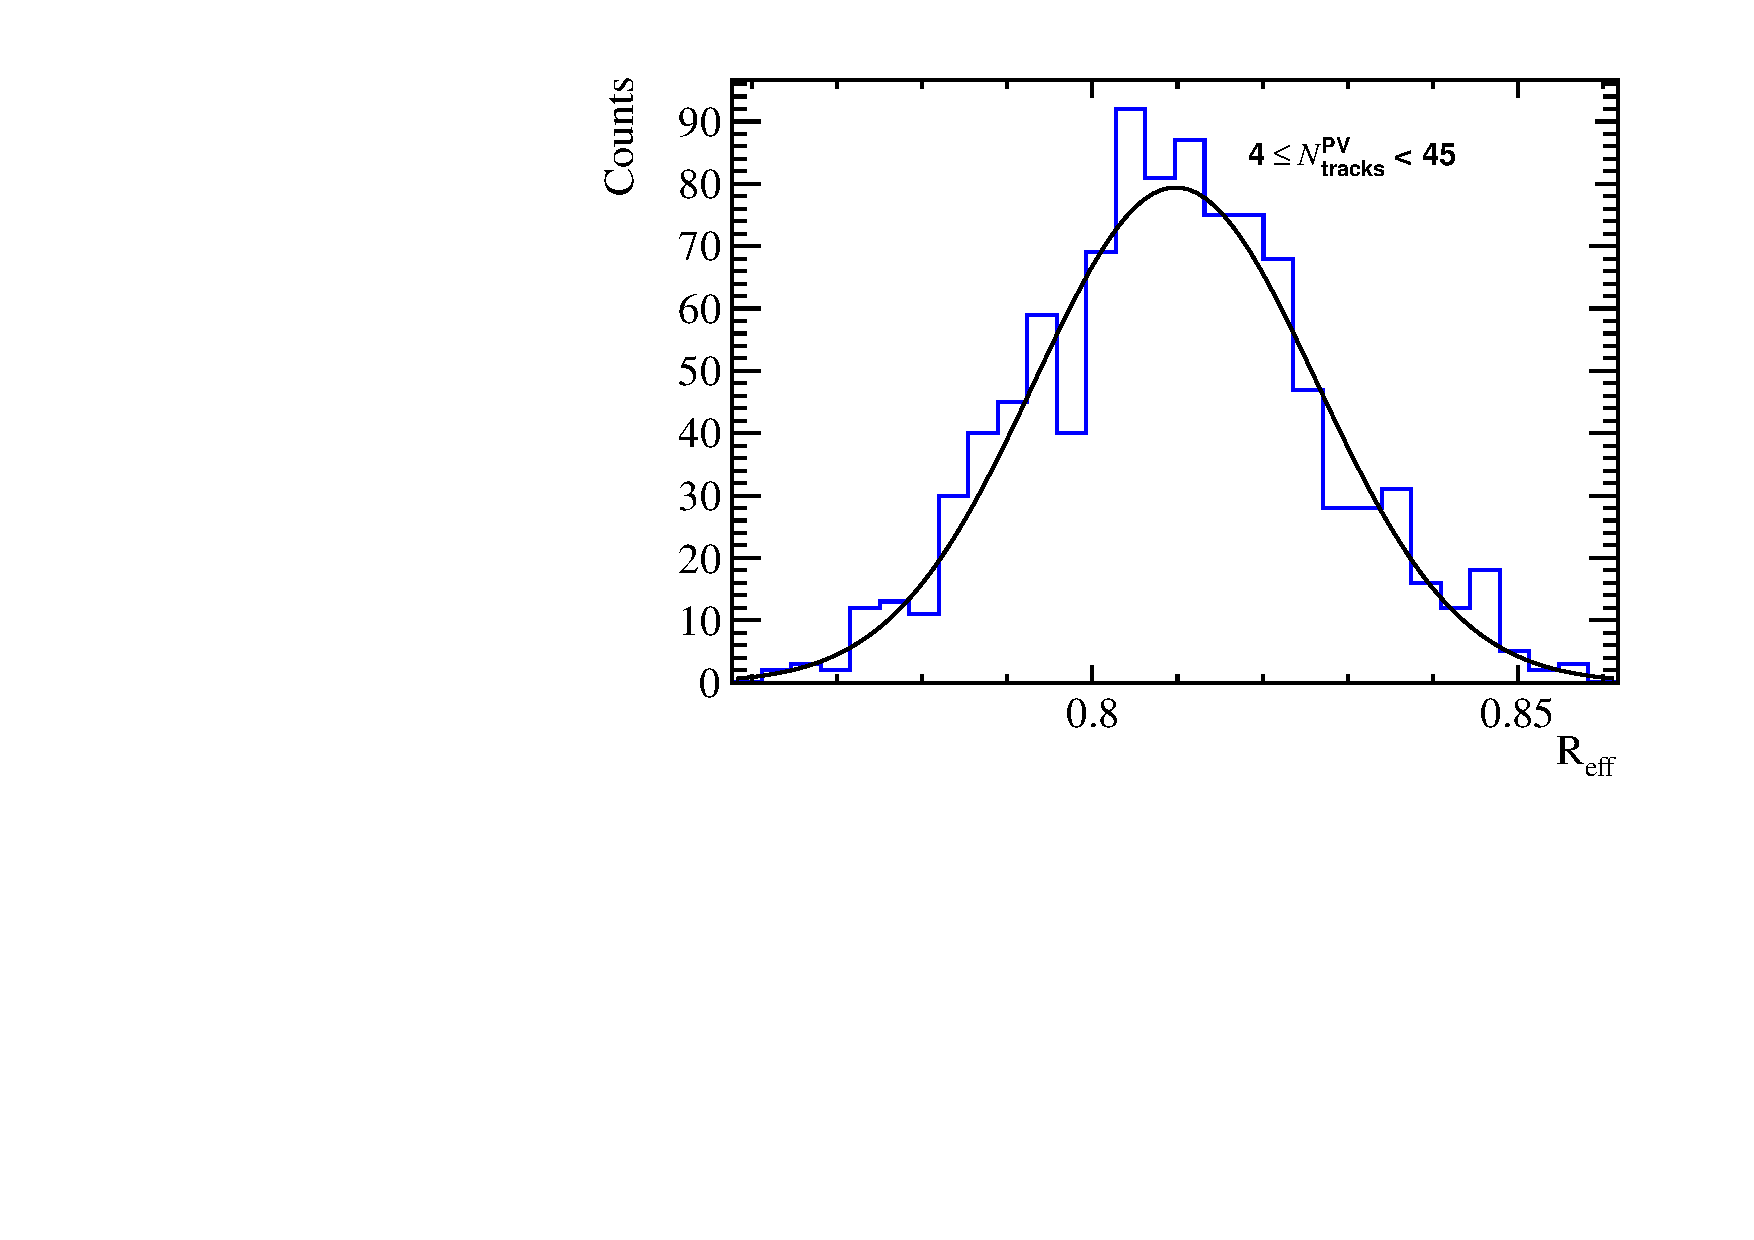
\includegraphics[width=0.49\linewidth]{pdf/pPb/Workdir/Eff_RecselPIDTrigger/n1.pdf}
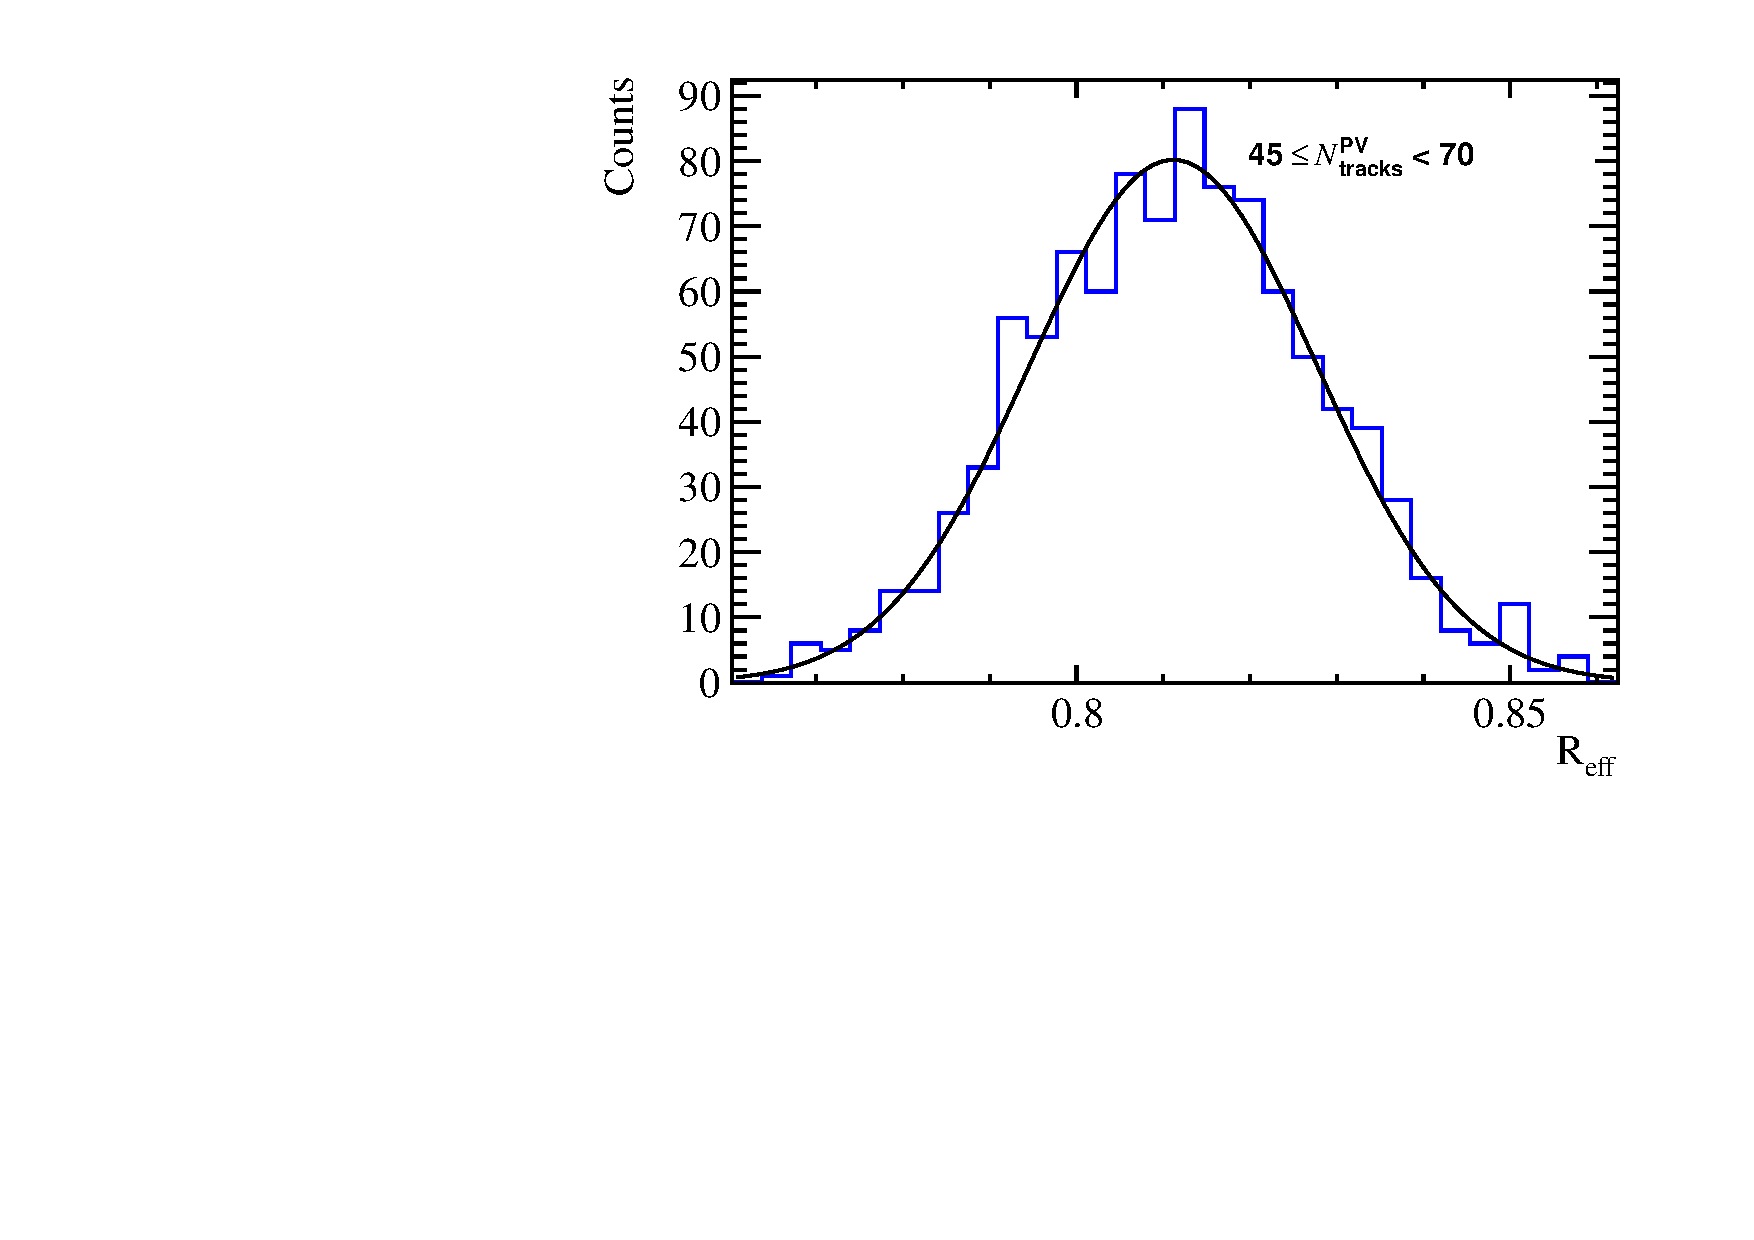
\includegraphics[width=0.49\linewidth]{pdf/pPb/Workdir/Eff_RecselPIDTrigger/n2.pdf}
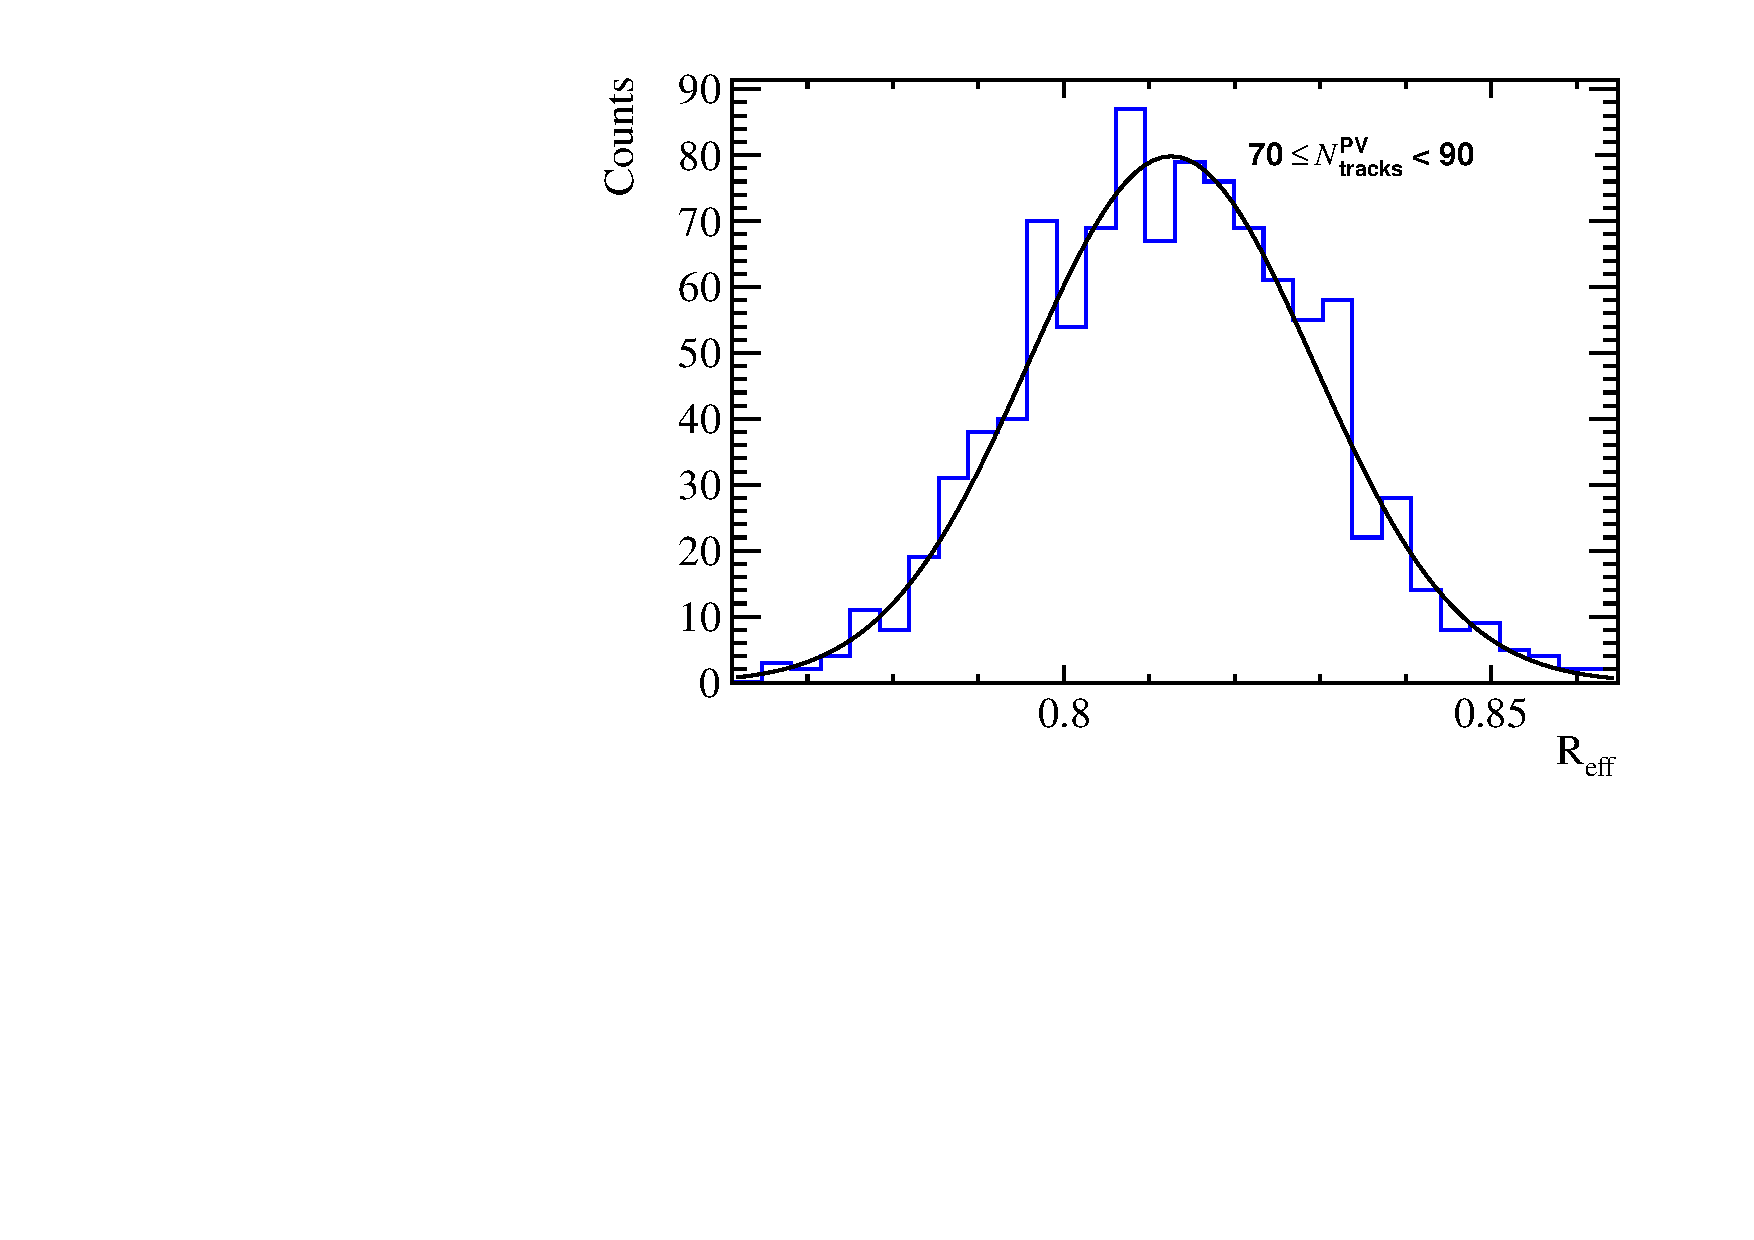
\includegraphics[width=0.49\linewidth]{pdf/pPb/Workdir/Eff_RecselPIDTrigger/n3.pdf}
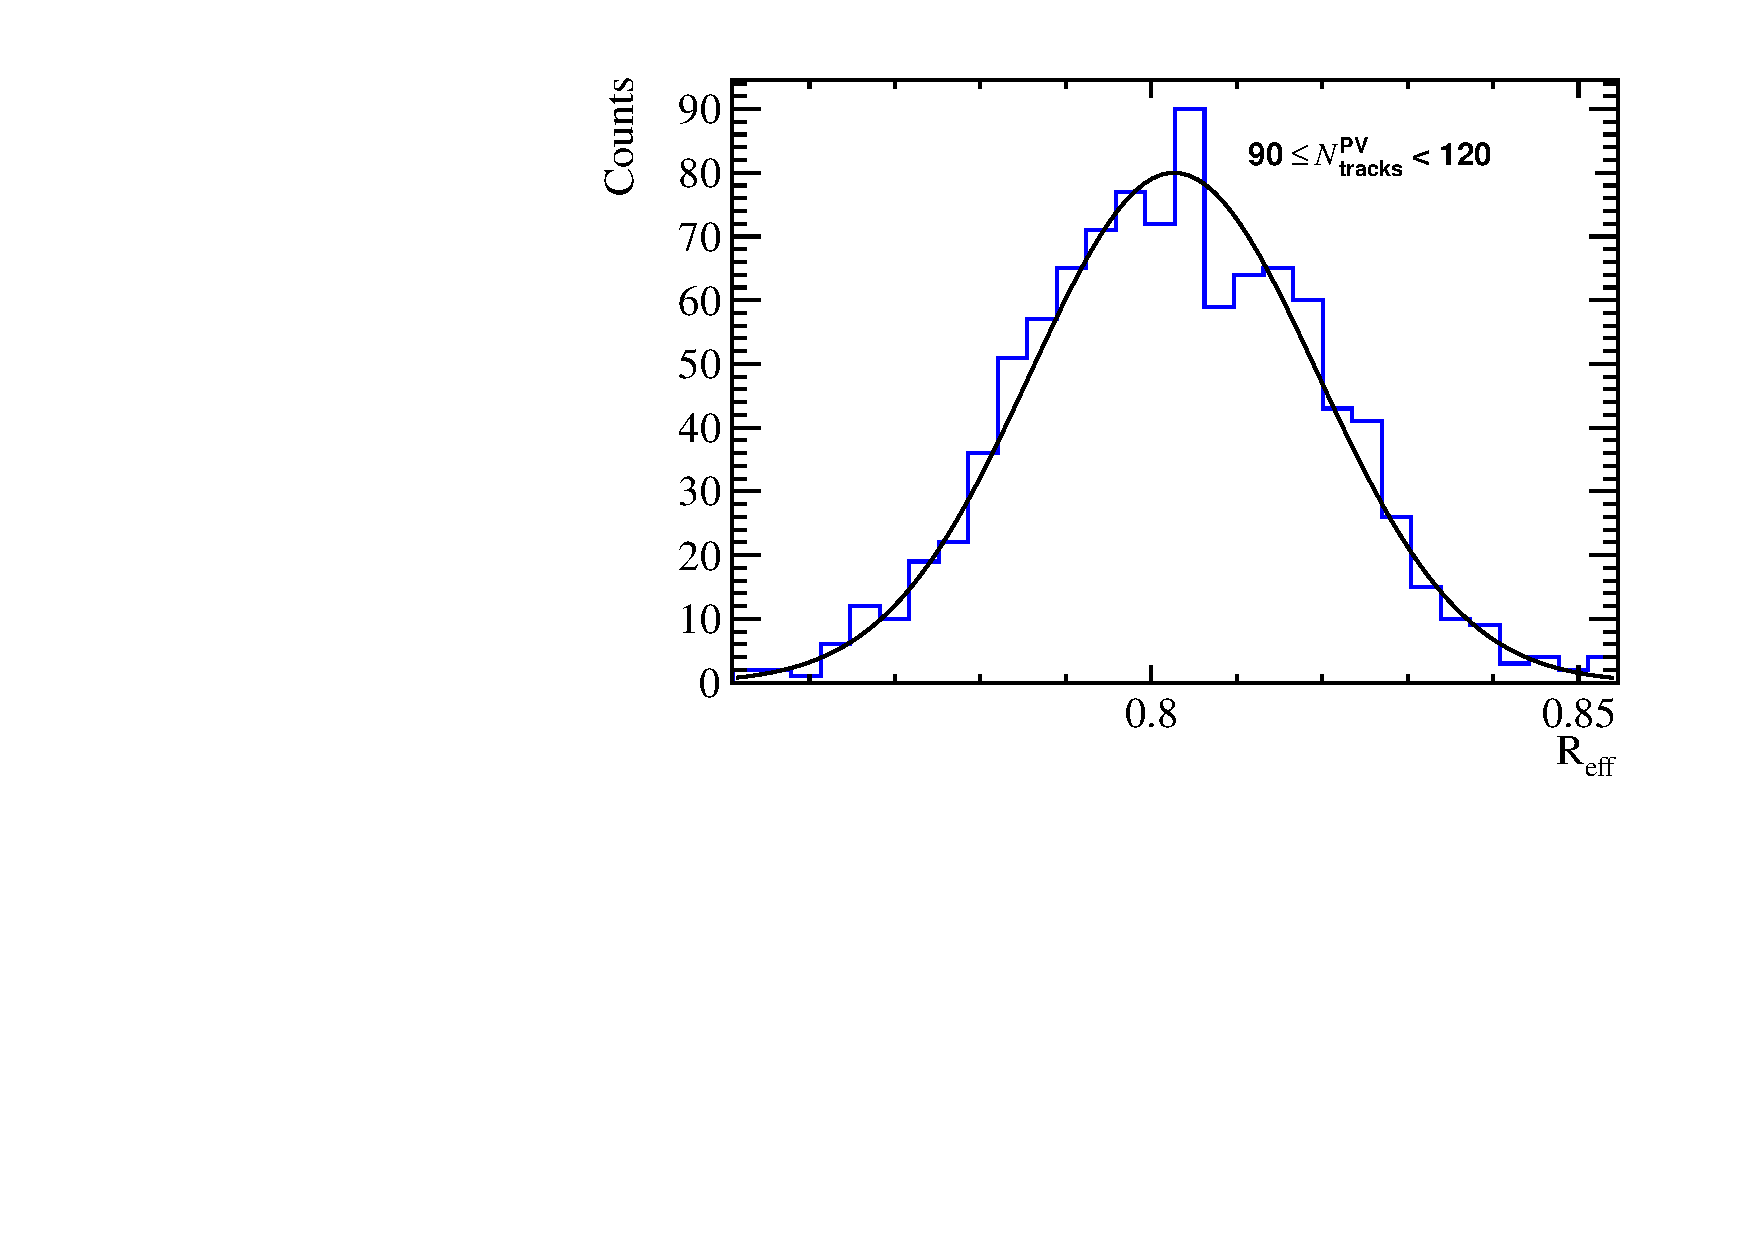
\includegraphics[width=0.49\linewidth]{pdf/pPb/Workdir/Eff_RecselPIDTrigger/n4.pdf}
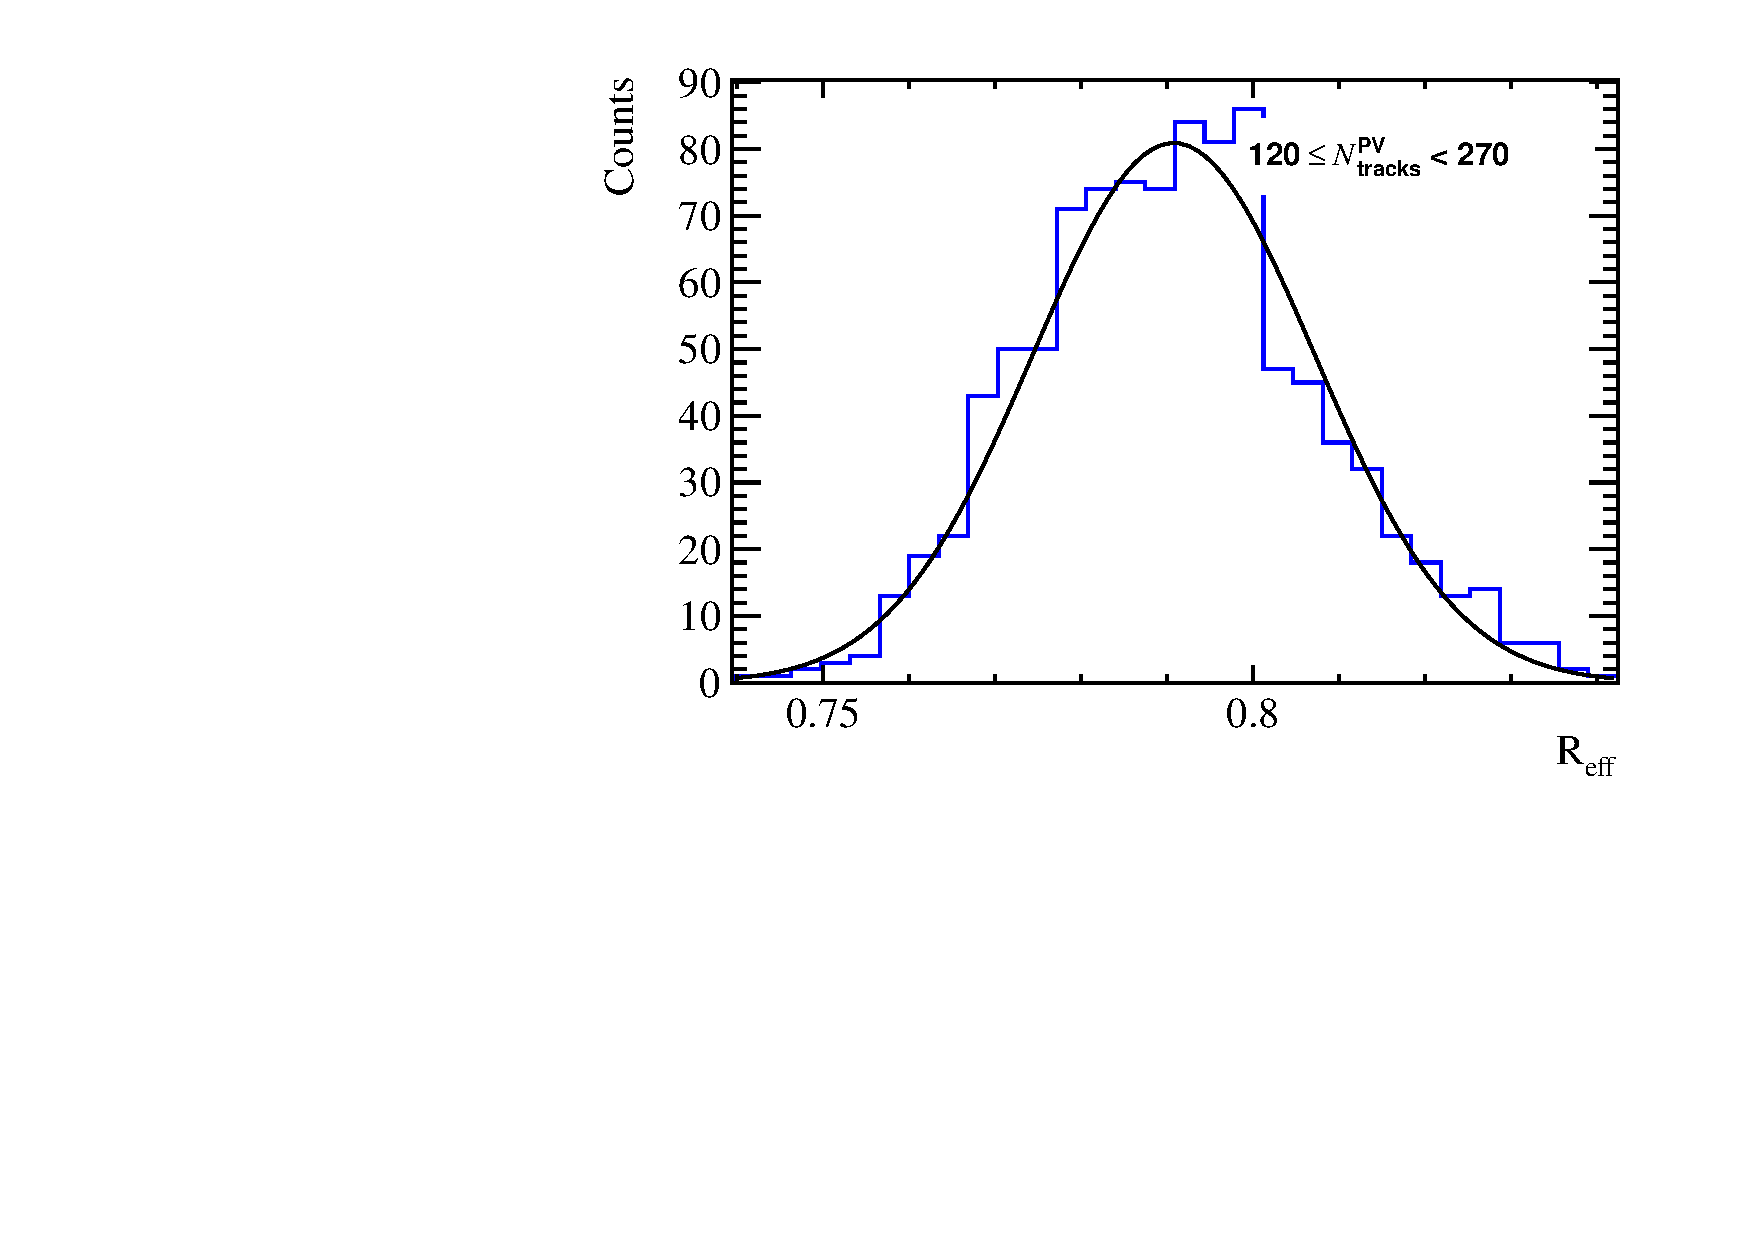
\includegraphics[width=0.49\linewidth]{pdf/pPb/Workdir/Eff_RecselPIDTrigger/n5.pdf}
\end{center}
\caption{
	Fit Gaussian functions on the distributions of 1000-trial $R_{eff}$ in different $N_{\rm tracks}^{\rm PV}$ bins in $p$Pb collisions.}
\label{ReffPlots}
\end{figure}


\begin{table}[H]
\centering
\caption{$R_{eff}$ in different $N_{\rm tracks}^{\rm PV}$ regions in $p$Pb configuration.}
\begin{center}
\begin{tabular}{c|c}
\hline
$4 \leq \mathrm{N_{\rm tracks}^{\rm PV}} < 45$ & $0.810 \pm 0.021$ \\
\hline
$45 \leq \mathrm{N_{\rm tracks}^{\rm PV}} < 70$ & $0.811 \pm 0.020$ \\
\hline
$70 \leq \mathrm{N_{\rm tracks}^{\rm PV}} < 90$ & $0.813 \pm 0.021$ \\
\hline
$90 \leq \mathrm{N_{\rm tracks}^{\rm PV}} < 120$ & $0.803 \pm 0.021$ \\
\hline
$120 \leq \mathrm{N_{\rm tracks}^{\rm PV}} < 270$ & $0.791 \pm 0.021$ \\
\hline
\end{tabular}
\end{center}
\label{ReffTable_PVNTRACKS_pPb}
\end{table}



%%%%%%%%%%%%%%%%%%%%%%%%%%%%%%%%%%%%%%%%%%%%%%%%%%%%%%%%%%%%%%%%%%%%%%%Uncertainty%%%%%%%%%%%%%%%%%%%%%%%%%%%%%%%%%%%%%%%%%%%%%%%%%%%%%%%%%%%%%%%%%%%%%%%%%%%%%%%%%%%%%%%
\section{Other Systematic uncertainties}
\label{Systematic uncertainty}
Before we proceed this section, we state some systematic uncertainties mentioned in previous sections, and add some conclusions on those which are simple to handle as follow,
\begin{itemize}
    \item re-weight of \pt distribution from high- and low-multiplicity samples (for ratios of \effAcc and the other efficiencies),
    \item re-weight of $y^*$ distribution from high- and low-multiplicity samples (for ratios of \effAcc and the other efficiencies),
    \item uncertainties due to the limit calibration sample size in PIDCalib efficiency table (for ratios of efficiencies except \effAcc),
    \item uncertainties of data-over-simulation ratio of per tracking efficiency(for ratios of efficiencies except \effAcc),
    \item global cut of nVeloClusters $<8000$ (negligible),
    \item uncertainty of luminosity is canceled when calculating the ratio of \psitwos-to-\jpsi production,
    \item relative uncertainty due to branching fraction is calculated to be $2.2\%$, this term is not considered when calculating the normalized ratio as function of multiplicity, but when we compare ratio in forward and backward regions, we do not normalize the ratio, hence, need to consider it in this case.
\end{itemize}

Other systematic uncertainties are reported in this section.
\subsection{Monte Carlo statistics}
This uncertainty is the statistical error on the ratio of efficiencies in different multiplicity bins, due to the finite size of the simulation samples. The uncertainty varies from $0.02\%$ to $0.2\%$ over all multiplicity classes divided by three multiplicity variables and in $p$Pb and Pb$p$ configurations, which is negligible compared to other systematic uncertainties.
\subsection{Signal extraction}
The choice of the fit model for the mass and $t_z$ distributions affects the number of events. In Sec~\ref{Signal extraction} we have mentioned that two CB functions with common mean are used for \jpsi mass fit while only one is used for \psitwos. The uncertainty associated with the choice of the signal mass function is estimated using a different function of two CB functions for \psitwos. Two CB functions have common mean, the $\alpha$ values for both CB functions are determined by the Eq.~\ref{alphasigma}. And the width of wider CB function is determined by $\sigma_2=sigma_1+25.7$, the ratio of the narrower one is fixed to 0.96 according to the study in 13.TeV $pp$ collisions~\cite{LHCb:2019eaj}.
New fit model for \psitwos mass spectrum is introduced and then a new two-dimensional fit for mass and $t_z$ is performed. Then the difference in ratio of \psitwos-to-\jpsi ratio and the statistical uncertainty of the ratio in each $N_{\rm tracks}^{\rm PV}$ bin are shown in Figure~\ref{StatsAndFit}.
\begin{figure}[H]
\begin{center}
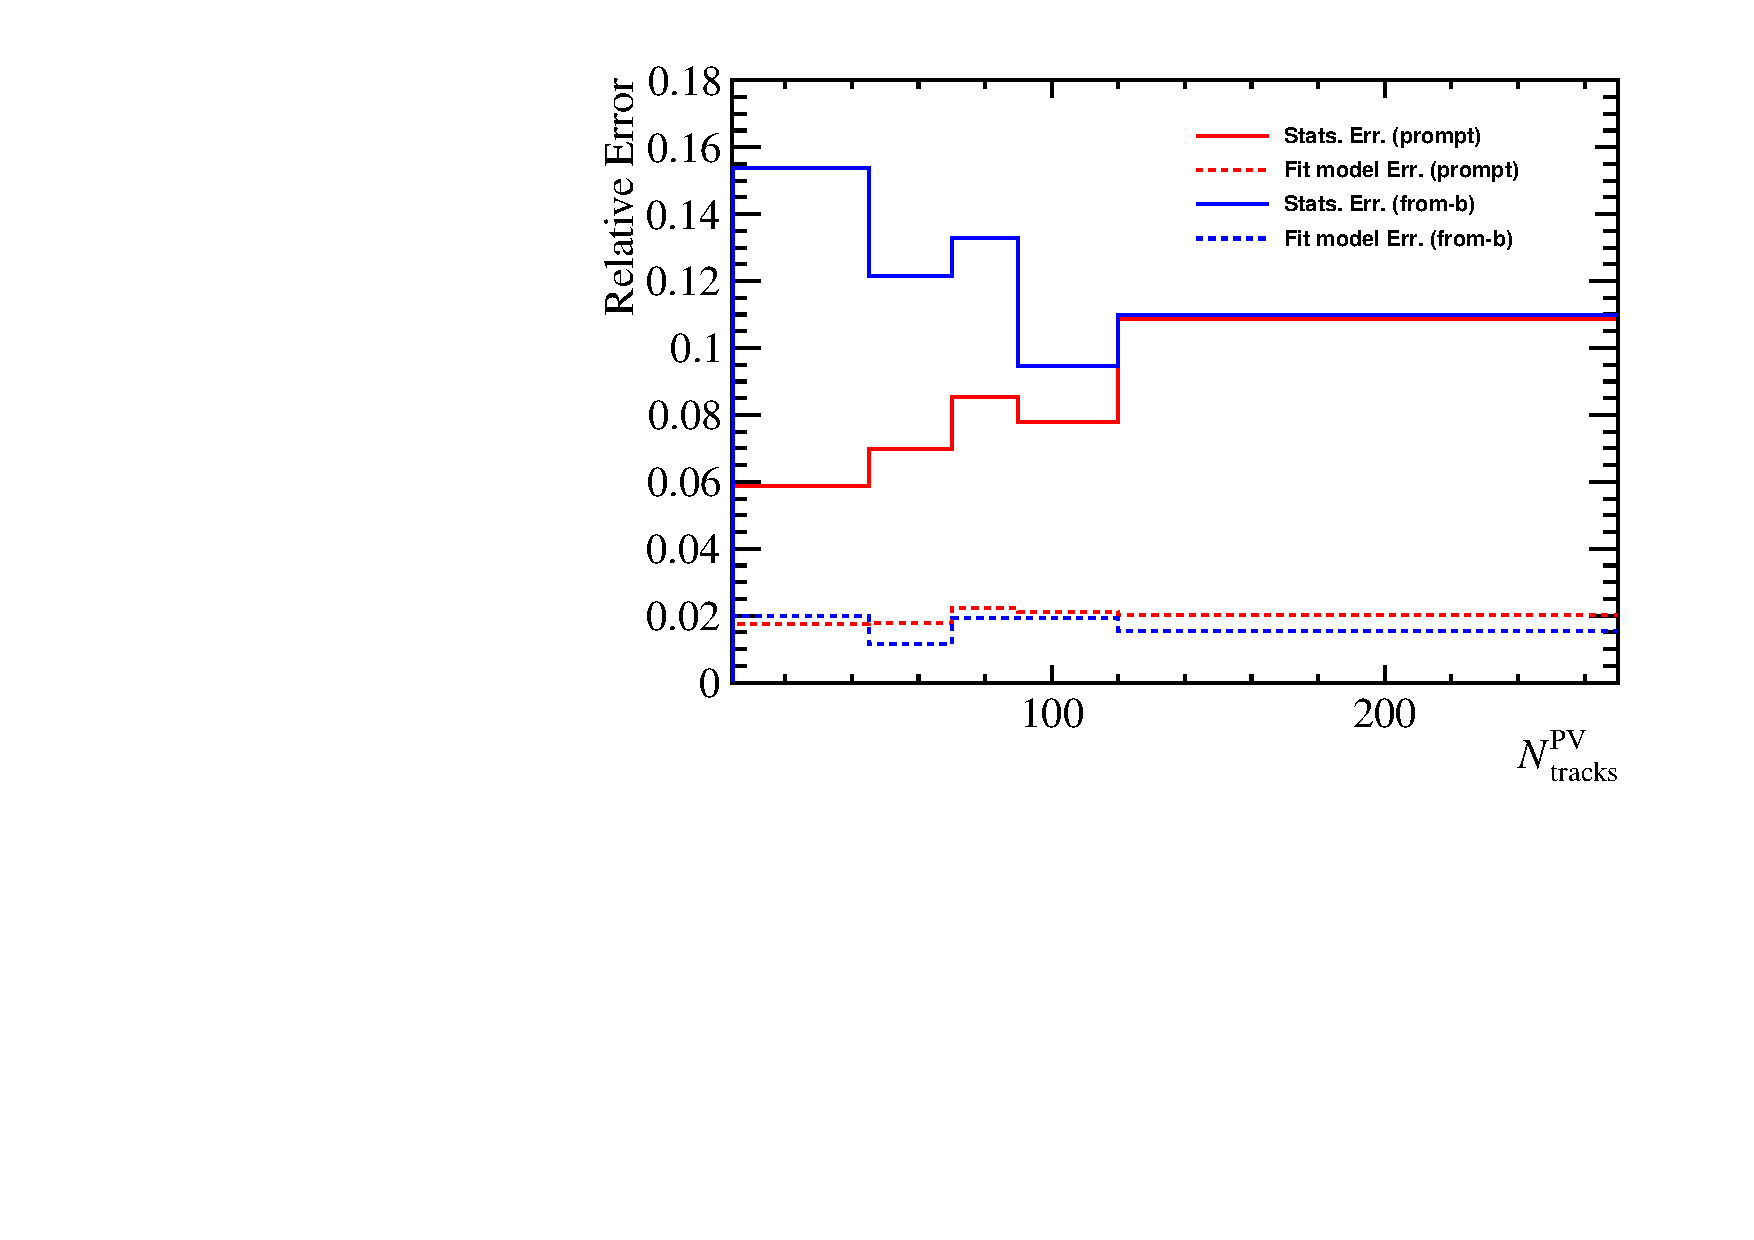
\includegraphics[width=0.7\linewidth]{pdf/pPb/Workdir/SysErr/FitModel.pdf}
\end{center}
\caption{
        The statistical uncertainties and the systematic uncertainty arised from different fit model of \psitwos-to-\jpsi ratio.}
\label{StatsAndFit}
\end{figure}
The variations caused by different fit model (dashed line) are totally overwhelmed by the statistical uncertainties (solid line), the statistical uncertainty is larger than the uncertainty caused by fit model by at least a factor of 3. Which means we can completely treat the difference caused by fit model as statistical fluctuation, hence, negligible.

\subsection{Trigger efficiency}
The trigger efficiency in simulation is cross-checked with data, and the resulting difference in the ratio of \effTrigger between simulation and data is quoted as a systematic uncertainty. If the statistical uncertainties of the ratio arised from fitting the TIS and TISTOS sample of \jpsi and \psitwos are larger, then it will be quoted as systematic uncertainty. 
For both L0Muon and Hlt1DiMuonHighMass the TISTOS method is used to evaluate the efficiency for L0Muon \&\& Hlt1DiMuonHighMass both in simulation and data. We use L0Global as the TIS line. As the data sample size is limited by the number of the TIS events of \psitwos sample, the TISTOS efficiencies are derived from data and Monte Carlo sample integrated over all multiplicity and kinematic region. Due to the different global cuts under different multiplicity schemes and configurations, TISTOS method is carried out in each case and the result is summarized in Table~\ref{TISTOStable}.
\begin{table}[H]
\caption{Systematic uncertainty of \effTrigger by TISTOS method.}
\begin{center}
\begin{tabular}{lllll}
\hline
\textbf{Configuration} & \textbf{Mult. Variable} & \textbf{Variation} & \textbf{Stats. Err.} & \textbf{Syst. Err. quoted}  \\
\hline
	$p$Pb & $N_{\rm tracks}^{\rm PV}$ & 2.7\% & 3.9\% & 3.9\%\\
	$p$Pb & $N_{\rm fwd}^{\rm PV}$ & 3.2\% & 3.0\% & 3.2\%\\
	$p$Pb & $N_{\rm bwd}^{\rm PV}$ & 2.7\% & 3.9\% & 3.9\% \\
        Pb$p$ & $N_{\rm tracks}^{\rm PV}$ & 2.0\% & 3.8\% & 3.8\% \\
        Pb$p$ & $N_{\rm fwd}^{\rm PV}$ &  1.7\% & 3.6\% & 3.6\%\\
        Pb$p$ & $N_{\rm bwd}^{\rm PV}$ &  2.7\% & 4.1\% & 4.1\%\\
\hline
\end{tabular}
\label{TISTOStable}
\end{center}
\end{table}
\subsection{Binning scheme of PID table}
Uncertainty due to binning scheme of the calibration sample, studied by varying the binning method in $p_\mu$, $\eta_\mu$, and nSPDHits respectively. The default one and the two alternative binning schemes could be found below. The nominal binning scheme of the muon ID efficiency for muons we use to calculate the muon ID efficiency of \jpsi and \psitwos mesons is defined:
\begin{itemize}
  \item $p_\mu$ boundaries [\gevc]: 3, 10, 20, 25, 30, 35, 40, 45, 50, 60, 70, 80, 100, 1000.
  \item $\eta$ boundaries: 2.0, 2.5, 3.0, 3.5, 4.0, 4.5, 5.0.
  \item nSPDhits boundaries: 0, 300, 500, 700, 1400.
\end{itemize}

One of the two alternative binning schemes is defined:
\begin{itemize}
  \item $p_\mu$ boundaries [\gevc]: 3, 12.5, 22.5, 27.5, 32.5, 37.5, 42.5, 47.5, 55, 65, 75, 85, 100, 1000.
  \item $\eta$ boundaries: 2.0, 2.6, 2.9, 3.6, 3.9, 4.5, 5.0.
  \item nSPDhits boundaries: 0, 250, 450, 650, 1400.
\end{itemize}

The other one binning schemes is defined:
\begin{itemize}
  \item $p_\mu$ boundaries [\gevc]: 3, 9, 19, 24, 29, 34, 39, 44, 49, 59, 69, 79, 100, 1000.
  \item $\eta$ boundaries: 2.0, 2.4, 3.1, 3.4, 3.9, 4.5, 5.0.
  \item nSPDhits boundaries: 0, 320, 480, 720, 1400.
\end{itemize}
The maximum difference between the two new ratios calculated and the nominal ratio is quoted as the systematic uncertainty. The uncertainties are from 0.1\% to 1.8\%.

\subsection{Summary of systematic uncertainties}
All the systematic uncertainties are summarized in Table~\ref{AllSysErr}.
\begin{table}[H]
\caption{Summary of systematic uncertainties on \psitwos-to-\jpsi cross-section ratio.}
\begin{center}
\begin{tabular}{llll}
\hline
\textbf{source} & \textbf{$p$Pb} & \textbf{Pb$p$} \\
\hline
L0\&HLT & 3.2\%-3.9\% & 3.6\%-4.1\% \\
\hline
	Tracking Table Uncertainty\& & & \\
	PID Table Uncertainty\& & & \\
	\pt spectrum\& & & \\
	$y$ spectrum & 1.7\%-3.6\% & 2.1\%-3.6\% \\
\hline
	PID Table scheme & 0.4\%-1.7\% & 0.1\%-1.8\% \\
\hline
	Imperfectly simulating acceptance & 0.8\%-1.2\% & 0.9\%-1.3\% \\
\hline
	$\frac{\BR(\jpsi\rightarrow\mu^+\mu^-)}{\BR(\psitwos\rightarrow\mu^+\mu^-}$(canceled if normalized) & 2.2\% &2.2\% \\
\hline
	Fit model & negligible & negligible \\
\hline
	MC sample size & negligible & negligible \\
\hline
	Multiplicity global cut & negligible & negligible \\
\hline
\end{tabular}
\label{AllSysErr}
\end{center}
\end{table}


%%%%%%%%%%%%%%%%%%%%%%%%%%%%%%%%%%%%%%%%%%%%%%%%%%%%%%%%%%%%%%%%%%%%%%%%%Result%%%%%%%%%%%%%%%%%%%%%%%%%%%%%%%%%%%%%%%%%%%%%%%%%%%%%%%%%%%%%%%%%%%%%%%%%%%%%%%%%%%%%%%%%%
\section{Results}
\label{Results}
\subsection{\psitwos-to-\jpsi ratio as function of multiplicity}
With the signal yields determined from the fitting to dimuon invariant mass distributions, the efficiency ratios estimated from simulation and calibrated control samples, and the systematic uncertainties, the ratio of \psitwos and \jpsi production cross-sections are measured as a function of different multiplicity variables. As mentioned in Sec~\ref{Efficiency determination}, the multiplicity distribution of \jpsi and \psitwos can be treated as the same, and due to the large uncertainty of \psitwos multiplicity distribution, the x-coordinate representing the multiplicity is directly the mean value of \jpsi multiplicity distribution in each bin, normalized by the mean value of multiplicity of NoBias data. The box represents systematic uncertainty and the error bar represents the statistical uncertainty. In this analysis statistical uncertainty dominates.
The normalized \psitwos-to-\jpsi ratio as function of $N_{\rm tracks}^{\rm PV}$ in $p$Pb and Pb$p$ collisions is shown in Figure~\ref{NormPVN}.
\begin{figure}[H]
\begin{center}
\includegraphics[width=0.49\linewidth]{pdf/pPb/Workdir/Result/All.pdf}
\includegraphics[width=0.49\linewidth]{pdf/Pbp/Workdir/Result/All.pdf}
\end{center}
\caption{Normalized \psitwos-to-\jpsi ratio as function of normalized $N_{\rm tracks}^{\rm PV}$ in $p$Pb (left) Pb$p$ (right).}
\label{NormPVN}
\end{figure}
We can conclude that in $p$Pb collisions the prompt ratio decrease with increasing $N_{\rm tracks}^{\rm PV}$, while in Pb$p$ collisions, we can not conclude any significant trend with $N_{\rm tracks}^{\rm PV}$. For \jpsi and \psitwos from $b$ we do not find any dependence between the ratio and multiplicity.
If we compare the prompt ratio (not normalized), we should include the uncertainties due to the branching fraction and the comparison is in Figure~\ref{ComparePVN}.
\begin{figure}[H]
\begin{center}
\includegraphics[width=0.7\linewidth]{pdf/pPb/Workdir/Result/Norm.pdf}
\end{center}
\caption{\psitwos-to-\jpsi ratio as function of normalized $N_{\rm tracks}^{\rm PV}$.}
\label{ComparePVN}
\end{figure}
We find the ratio in Pb$p$ is generally lower than that in $p$Pb collisions. This could results from the higher charged particle multiplicity in Pb$p$ collisions, where \psitwos, with lower binding energy, is easier to dissociate when interacting with higher amount of co-moving particles. But if this is valid, we should also observe a decreasing trend of the ratio with increasing multiplicity, which is indeed not seen.
We further measure the normalized ratio and ratio as functions of $N_{\rm fwd}^{\rm PV}$, as shown in Figure~\ref{NormFor}. It agrees with the results when measuring by $N_{\rm tracks}^{\rm PV}$. The ratio of non-prompt signals is roughly constant with multiplicity in $p$Pb and Pb$p$ collisions. And ratio of prompt signals decreases with increasing $N_{\rm fwd}^{\rm PV}$ in $p$Pb, but not in Pb$p$ collisions. 
If we compare the ratio in $p$Pb and Pb$p$ collisions, the ratios in Pb$p$ collisions are generally lower than that in p$Pb$ collisions. But still, we do not observe a decreasing trend like in $p$Pb collisions. Some extra mechanisms might be needed to explain the phenomenon. Since for both $N_{\rm tracks}^{\rm PV}$ and $N_{\rm fwd}^{\rm PV}$ as multiplicity variables, we get the similar outcomes.
\begin{figure}[H]
\begin{center}
\includegraphics[width=0.49\linewidth]{pdf/pPb/FWorkdir/Result/All.pdf}
\includegraphics[width=0.49\linewidth]{pdf/Pbp/FWorkdir/Result/All.pdf}
\includegraphics[width=0.7\linewidth]{pdf/pPb/FWorkdir/Result/Norm.pdf}
\end{center}
\caption{Normalized \psitwos-to-\jpsi ratio as function of normalized $N_{\rm fwd}^{\rm PV}$ in $p$Pb (left) Pb$p$ (right).}
\label{NormFor}
\end{figure}
When multiplicity is measured by $N_{\rm bwd}^{\rm PV}$, as shown in Figure~\ref{NormBack}, for ratio of prompt signals, the decreasing trend is much slower with increasing $N_{\rm bwd}^{\rm PV}$ in $p$Pb collisions, and for Pb$p$, the ratio for both prompt and non-prompt signals are roughly constant. Since the $N_{\rm bwd}^{\rm PV}$ are measured in backward direction, where the rapidity range is non-overlapping with charmonia measurements, no decreasing trend will be observed due to comover effect. Additionally, if QGP is not produced, the ratio should keep constant with $N_{\rm bwd}^{\rm PV}$. The subtle decreasing trend for ratio of prompt signals could result from the correlation between $N_{\rm bwd}^{\rm PV}$ and  $N_{\rm fwd}^{\rm PV}$ in $p$Pb collisions. Similarly, there is an overall reduction on the ratio in Pb$p$ collisions since the mean value of charged particle multiplicity is higher, which results in an overall larger amount of co-moving particles. But still, in Pb$p$ collisions, no dependence was found between ratio and $N_{\rm bwd}^{\rm PV}$.
\begin{figure}[H]
\begin{center}
\includegraphics[width=0.49\linewidth]{pdf/pPb/BWorkdir/Result/All.pdf}
\includegraphics[width=0.49\linewidth]{pdf/Pbp/BWorkdir/Result/All.pdf}
\includegraphics[width=0.7\linewidth]{pdf/pPb/BWorkdir/Result/Norm.pdf}
\end{center}
\caption{Normalized \psitwos-to-\jpsi ratio as function of normalized $N_{\rm bwd}^{\rm PV}$ in $p$Pb (left) Pb$p$ (right).}
\label{NormBack}
\end{figure}

\subsection{Comparison in different collision systems}
The multiplicity dependence of \psitwos to \jpsi ratio in different collision systems is compared as shown in Fig~\ref{pppPb}. 
\begin{figure}[H]
  \begin{center}
  \includegraphics[width=0.7\linewidth]{LHCb-latex-template/latest/latex/pdf/pPb/FWorkdir/Result/pppPb.pdf}
  \end{center}
  \caption{Comparisons on the ratio of \psitwos/\jpsi in $pp$, $p$Pb (Pb$p$) and PbPb collisions~\cite{ALICE:2022jeh}.}
\label{pppPb}
\end{figure}
The multiplicity dependence in $p$Pb collisions is consistent with that in $pp$ result, suggesting a similar environment in the final stages in both collision systems. It is within expectation since both are measured in the $p$ going direction, suggesting a similar environment. However, in Pb$p$ collisions, where the charmonia and multiplicity are measured in the $Pb$-going direction, a higher baryon density will achieve, resulting in an environment closer to PbPb collisions. Therefore, a slower decreasing trend is observed in Pb$p$ collisions, which is very close to the result in PbPb collisions measured by ALICE~\cite{ALICE:2022jeh}. A transition phenomenon from small collision systems to large systems is observed.


%%%%%%%%%%%%%%%%%%%%%%%%%%%%%%%%%%%%%%%%%%%%%%%%%%%%%%%%%%%%%%%%%%%%%Conclusion%%%%%%%%%%%%%%%%%%%%%%%%%%%%%%%%%%%%%%%%%%%%%%%%%%%%%%%%%%%%%%%%%%%%%%%%%%%%%%%%%%%%%%%%%%
\section{Conclusion}
\label{conclusion}
The ratio of production cross-sections of \psitwos to \jpsi in $p$Pb and Pb$p$ collisions at a center-of-mass energy $\sqrt{s_{NN}}=8.16\tev$ are reported with a data sample corresponding to an integrated luminosity of $13.6\pm0.3$nb$^{-1}$ for $p$Pb and $20.8\pm0.5$nb$^{-1}$ for Pb$p$ collected by the \lhcb detector in 2016. The (normalized) ratios of prompt and non-prompt \psitwos-to-\jpsi production, as functions of different multiplicity variables, are measured in region of $0\gev<\pt<14\gev$ and $1.5<y^*<4.5$ for $p$Pb and $-5.5<y^*<-2.5$ for Pb$p$. In $p$Pb collisions, we see an obvious decreasing trend for ratio of prompt production as a function of $N_{\rm tracks}^{\rm PV}$ and $N_{\rm fwd}^{\rm PV}$ in $p$Pb and a slower decrease as a function of $N_{\rm bwd}^{\rm PV}$. In Pb$p$ collisions, even though the ratios have an overall lower value compared to $p$Pb with same multiplicity scheme, the prompt and non-prompt \psitwos-to-\jpsi ratio does not show an obvious decrease as in $p$Pb. The overall ratios in $p$Pb and Pb$p$ show good agreements with other measurements in different collision systems at different energies.





\appendix
\clearpage
\section{Table of ratios}
\label{Table of ratios}
In the appendix, we attach the ratios only, one can easily get the normalized ratios by simple calculations. Remember to cut off 2.2$\%$ relative systematic uncertainties from uncertainties of branching ratios.
\begin{table}[H]
\caption{Ratio(\%) of production cross-section for \psitwos to \jpsi. The first uncertainties are statistical, the second are the systematic uncertainties.}
\centering
\resizebox{\linewidth}{!}{
\begin{tabular}{|c|c|c|c|c|c|}
\hline
\multicolumn{6}{|c|}{$p$Pb}\\\hline
$N_{\rm tracks}^{\rm PV}$ & \ 4\~45 & 45\~70 & 70\~90 & 90\~120 & 120\~270 \\
\hline
prompt & $0.172\pm0.010\pm0.008$ & $0.142\pm0.010\pm0.006$ & $0.112\pm0.010\pm0.005$ & $0.124\pm0.010\pm0.006$ & $0.101\pm0.011\pm0.005$ \\
\hline
non-prompt & $0.219\pm0.034\pm0.012$ & $0.230\pm0.028\pm0.011$ & $0.195\pm0.026\pm0.009$ & $0.265\pm0.025\pm0.011$ & $0.243\pm0.027\pm0.010$ \\
\hline
\multicolumn{6}{|c|}{Pb$p$}\\\hline
$N_{\rm tracks}^{\rm PV}$ & \ 4\~60 & 60\~90 & 90\~120 & 120\~160 & 160\~330 \\
\hline
prompt & $0.118\pm0.006\pm0.006$ & $0.093\pm0.006\pm0.004$ & $0.112\pm0.008\pm0.005$ & $0.090\pm0.009\pm0.004$ & $0.126\pm0.017\pm0.006$ \\
\hline
non-prompt & $0.240\pm0.023\pm0.012$ & $0.193\pm0.021\pm0.009$ & $0.197\pm0.020\pm0.010$ & $0.216\pm0.022\pm0.009$ & $0.304\pm0.040\pm0.013$ \\
\hline
\end{tabular}
}
\label{RatioPVN}
\end{table}

\begin{table}[H]
\caption{Ratio(\%) of production cross-section for \psitwos to \jpsi. The first uncertainties are statistical, the second are the systematic uncertainties.}
\centering
\resizebox{\linewidth}{!}{
\begin{tabular}{|c|c|c|c|c|c|}
\hline
\multicolumn{6}{|c|}{$p$Pb}\\\hline
$N_{\rm fwd}^{\rm PV}$ & \ 0~25 & 25~43 & 43~57 & 57~72 & 72~150 \\
\hline
prompt & $0.183\pm0.010\pm0.007$ & $0.136\pm0.007\pm0.005$ & $0.144\pm0.008\pm0.005$ & $0.111\pm0.008\pm0.004$ & $0.114\pm0.008\pm0.004$ \\
\hline
non-prompt & $0.192\pm0.034\pm0.009$ & $0.236\pm0.021\pm0.009$ & $0.216\pm0.021\pm0.009$ & $0.262\pm0.022\pm0.009$ & $0.222\pm0.018\pm0.008$ \\
\hline
\multicolumn{6}{|c|}{Pb$p$}\\\hline
$N_{\rm fwd}^{\rm PV}$ & \ 0~35 & 35~65 & 65~85 & 85~110 & 110~250 \\
\hline
prompt & $0.121\pm0.006\pm0.006$ & $0.097\pm0.006\pm0.004$ & $0.104\pm0.007\pm0.004$ & $0.098\pm0.008\pm0.004$ & $0.099\pm0.012\pm0.004$ \\
\hline
non-prompt & $0.262\pm0.028\pm0.012$ & $0.199\pm0.018\pm0.009$ & $0.225\pm0.022\pm0.010$ & $0.198\pm0.021\pm0.009$ & $0.255\pm0.027\pm0.010$ \\
\hline
\end{tabular}
}
\label{RatioFor}
\end{table}

\begin{table}[H]
\caption{Ratio(\%) of production cross-section for \psitwos to \jpsi. The first uncertainties are statistical, the second are the systematic uncertainties.}
\centering
\resizebox{\linewidth}{!}{
\begin{tabular}{|c|c|c|c|c|c|}
\hline
\multicolumn{6}{|c|}{$p$Pb}\\\hline
$N_{\rm bwd}^{\rm PV}$ & \ 0~17 & 17~29 & 29~40 & 40~54 & 54~180 \\
\hline
prompt & $0.151\pm0.009\pm0.007$ & $0.120\pm0.009\pm0.005$ & $0.128\pm0.010\pm0.006$ & $0.132\pm0.012\pm0.006$ & $0.093\pm0.012\pm0.004$ \\
\hline
non-prompt & $0.219\pm0.027\pm0.011$ & $0.220\pm0.024\pm0.010$ & $0.238\pm0.026\pm0.011$ & $0.252\pm0.029\pm0.011$ & $0.242\pm0.033\pm0.009$ \\
\hline
\multicolumn{6}{|c|}{Pb$p$}\\\hline
$N_{\rm bwd}^{\rm PV}$ & \ 0~13 & 13~22 & 22~30 & 30~47 & 47~120 \\
\hline
prompt & $0.118\pm0.008\pm0.006$ & $0.103\pm0.008\pm0.005$ & $0.106\pm0.009\pm0.006$ & $0.097\pm0.008\pm0.005$ & $0.113\pm0.018\pm0.006$ \\
\hline
non-prompt & $0.209\pm0.032\pm0.012$ & $0.219\pm0.025\pm0.011$ & $0.217\pm0.024\pm0.012$ & $0.243\pm0.023\pm0.012$ & $0.239\pm0.041\pm0.012$ \\
\hline
\end{tabular}
}
\label{RatioBack}
\end{table}


\clearpage
\section{Table of efficiency ratios $R_eff$}
\begin{table}[H]
\centering
\caption{$R_{eff}$ in different $N_{\rm tracks}^{\rm PV}$ regions in $p$Pb configuration.}
\begin{center}
\begin{tabular}{c|c}
\hline
$4 \leq \mathrm{N_{\rm tracks}^{\rm PV}} < 45$ & $0.810 \pm 0.021$ \\
\hline
$45 \leq \mathrm{N_{\rm tracks}^{\rm PV}} < 70$ & $0.811 \pm 0.020$ \\
\hline
$70 \leq \mathrm{N_{\rm tracks}^{\rm PV}} < 90$ & $0.813 \pm 0.021$ \\
\hline
$90 \leq \mathrm{N_{\rm tracks}^{\rm PV}} < 120$ & $0.803 \pm 0.021$ \\
\hline
$120 \leq \mathrm{N_{\rm tracks}^{\rm PV}} < 270$ & $0.791 \pm 0.021$ \\
\hline
\end{tabular}
\end{center}
\label{ReffTable_PVN_pPb}
\end{table}

\begin{table}[H]
\centering
\caption{$R_{eff}$ in different $N_{\rm tracks}^{\rm PV}$ regions in $p$Pb configuration.}
\begin{center}
\begin{tabular}{c|c}
\hline
$0 \leq \mathrm{N_{\rm tracks}^{\rm PV}} < 17$ & $0.810 \pm 0.022$ \\
\hline
$17 \leq \mathrm{N_{\rm tracks}^{\rm PV}} < 29$ & $0.808 \pm 0.022$ \\
\hline
$29 \leq \mathrm{N_{\rm tracks}^{\rm PV}} < 40$ & $0.809 \pm 0.022$ \\
\hline
$40 \leq \mathrm{N_{\rm tracks}^{\rm PV}} < 54$ & $0.800 \pm 0.022$ \\
\hline
$54 \leq \mathrm{N_{\rm tracks}^{\rm PV}} < 140$ & $0.795 \pm 0.022$ \\
\hline
\end{tabular}
\end{center}
\label{ReffTable_NBack_pPb}
\end{table}

\input{Table/Eff/Eff_Nfor.tex}
\begin{table}[H]
\centering
\caption{$R_{eff}$ in different $N_{\rm tracks}^{\rm PV}$ regions in Pb$p$ configuration.}
\begin{center}
\begin{tabular}{c|c}
\hline
$0 \leq \mathrm{N_{\rm tracks}^{\rm PV}} < 60$ & $0.814 \pm 0.024$ \\
\hline
$60 \leq \mathrm{N_{\rm tracks}^{\rm PV}} < 90$ & $0.806 \pm 0.023$ \\
\hline
$90 \leq \mathrm{N_{\rm tracks}^{\rm PV}} < 120$ & $0.789 \pm 0.022$ \\
\hline
$120 \leq \mathrm{N_{\rm tracks}^{\rm PV}} < 160$ & $0.773 \pm 0.022$ \\
\hline
$160 \leq \mathrm{N_{\rm tracks}^{\rm PV}} < 330$ & $0.727 \pm 0.024$ \\
\hline
\end{tabular}
\end{center}
\label{ReffTable_PVN_Pbp}
\end{table}

\begin{table}[H]
\centering
\caption{$R_{eff}$ in different $N_{\rm tracks}^{\rm PV}$ regions in Pb$p$ configuration.}
\begin{center}
\begin{tabular}{c|c}
\hline
$0 \leq \mathrm{N_{\rm tracks}^{\rm PV}} < 13$ & $0.826 \pm 0.026$ \\
\hline
$13 \leq \mathrm{N_{\rm tracks}^{\rm PV}} < 22$ & $0.793 \pm 0.027$ \\
\hline
$22 \leq \mathrm{N_{\rm tracks}^{\rm PV}} < 30$ & $0.789 \pm 0.029$ \\
\hline
$30 \leq \mathrm{N_{\rm tracks}^{\rm PV}} < 47$ & $0.773 \pm 0.028$ \\
\hline
$47 \leq \mathrm{N_{\rm tracks}^{\rm PV}} < 100$ & $0.740 \pm 0.027$ \\
\hline
\end{tabular}
\end{center}
\label{ReffTable_NBack_Pbp}
\end{table}

\input{Table/Eff/PbpEff_Nfor.tex}

\clearpage
\section{Fit plots}
Two-dimensional fit for $p$Pb collisions:
\label{Fit plots}
\begin{figure}[H]
\begin{center}
\includegraphics[width=0.45\linewidth]{pdf/pPb/Workdir/TwoDimFit/ProjMass/Jpsi_n1y1pt1.pdf}
\includegraphics[width=0.45\linewidth]{pdf/pPb/Workdir/TwoDimFit/ProjTz/Jpsi_n1y1pt1.pdf}
\vspace*{-0.5cm}
\includegraphics[width=0.45\linewidth]{pdf/pPb/Workdir/TwoDimFit/ProjMass/Psi2S_n1y1pt1.pdf}
\includegraphics[width=0.45\linewidth]{pdf/pPb/Workdir/TwoDimFit/ProjTz/Psi2S_n1y1pt1.pdf}
\vspace*{-0.5cm}
\end{center}
\caption{Fit results in $0\gevc<\pt<14\gevc$, $1.5<y^*<4.5$ and 4$\leq$$N_{\rm tracks}^{\rm PV}$$<$45.}
\end{figure}
\begin{figure}[H]
\begin{center}
\includegraphics[width=0.45\linewidth]{pdf/pPb/Workdir/TwoDimFit/ProjMass/Jpsi_n2y1pt1.pdf}
\includegraphics[width=0.45\linewidth]{pdf/pPb/Workdir/TwoDimFit/ProjTz/Jpsi_n2y1pt1.pdf}
\vspace*{-0.5cm}
\includegraphics[width=0.45\linewidth]{pdf/pPb/Workdir/TwoDimFit/ProjMass/Psi2S_n2y1pt1.pdf}
\includegraphics[width=0.45\linewidth]{pdf/pPb/Workdir/TwoDimFit/ProjTz/Psi2S_n2y1pt1.pdf}
\vspace*{-0.5cm}
\end{center}
\caption{Fit results in $0\gevc<\pt<14\gevc$, $1.5<y^*<4.5$ and 45$\leq$$N_{\rm tracks}^{\rm PV}$$<70$.}
\end{figure}
\begin{figure}[H]
\begin{center}
\includegraphics[width=0.45\linewidth]{pdf/pPb/Workdir/TwoDimFit/ProjMass/Jpsi_n3y1pt1.pdf}
\includegraphics[width=0.45\linewidth]{pdf/pPb/Workdir/TwoDimFit/ProjTz/Jpsi_n3y1pt1.pdf}
\vspace*{-0.5cm}
\includegraphics[width=0.45\linewidth]{pdf/pPb/Workdir/TwoDimFit/ProjMass/Psi2S_n3y1pt1.pdf}
\includegraphics[width=0.45\linewidth]{pdf/pPb/Workdir/TwoDimFit/ProjTz/Psi2S_n3y1pt1.pdf}
\vspace*{-0.5cm}
\end{center}
\caption{Fit results in $0\gevc<\pt<14\gevc$, $1.5<y^*<4.5$ and 70$\leq$$N_{\rm tracks}^{\rm PV}$$<$90.}
\end{figure}
\begin{figure}[H]
\begin{center}
\includegraphics[width=0.45\linewidth]{pdf/pPb/Workdir/TwoDimFit/ProjMass/Jpsi_n4y1pt1.pdf}
\includegraphics[width=0.45\linewidth]{pdf/pPb/Workdir/TwoDimFit/ProjTz/Jpsi_n4y1pt1.pdf}
\vspace*{-0.5cm}
\includegraphics[width=0.45\linewidth]{pdf/pPb/Workdir/TwoDimFit/ProjMass/Psi2S_n4y1pt1.pdf}
\includegraphics[width=0.45\linewidth]{pdf/pPb/Workdir/TwoDimFit/ProjTz/Psi2S_n4y1pt1.pdf}
\vspace*{-0.5cm}
\end{center}
\caption{Fit results in $0\gevc<\pt<14\gevc$, $1.5<y^*<4.5$ and 90$\leq$$N_{\rm tracks}^{\rm PV}$$<$120.}
\end{figure}
\begin{figure}[H]
\begin{center}
\includegraphics[width=0.45\linewidth]{pdf/pPb/Workdir/TwoDimFit/ProjMass/Jpsi_n5y1pt1.pdf}
\includegraphics[width=0.45\linewidth]{pdf/pPb/Workdir/TwoDimFit/ProjTz/Jpsi_n5y1pt1.pdf}
\vspace*{-0.5cm}
\includegraphics[width=0.45\linewidth]{pdf/pPb/Workdir/TwoDimFit/ProjMass/Psi2S_n5y1pt1.pdf}
\includegraphics[width=0.45\linewidth]{pdf/pPb/Workdir/TwoDimFit/ProjTz/Psi2S_n5y1pt1.pdf}
\vspace*{-0.5cm}
\end{center}
\caption{Fit results in $0\gevc<\pt<14\gevc$, $1.5<y^*<4.5$ and 120$\leq$$N_{\rm tracks}^{\rm PV}$$<$270.}
\end{figure}

\begin{figure}[H]
\begin{center}
\includegraphics[width=0.45\linewidth]{pdf/pPb/FWorkdir/TwoDimFit/ProjMass/Jpsi_n1y1pt1.pdf}
\includegraphics[width=0.45\linewidth]{pdf/pPb/FWorkdir/TwoDimFit/ProjTz/Jpsi_n1y1pt1.pdf}
\vspace*{-0.5cm}
\includegraphics[width=0.45\linewidth]{pdf/pPb/FWorkdir/TwoDimFit/ProjMass/Psi2S_n1y1pt1.pdf}
\includegraphics[width=0.45\linewidth]{pdf/pPb/FWorkdir/TwoDimFit/ProjTz/Psi2S_n1y1pt1.pdf}
\vspace*{-0.5cm}
\end{center}
\caption{Fit results in $0\gevc<\pt<14\gevc$, $1.5<y^*<4.5$ and 0$\leq$$N_{\rm fwd}^{\rm PV}$$<$25.}
\end{figure}
\begin{figure}[H]
\begin{center}
\includegraphics[width=0.45\linewidth]{pdf/pPb/FWorkdir/TwoDimFit/ProjMass/Jpsi_n2y1pt1.pdf}
\includegraphics[width=0.45\linewidth]{pdf/pPb/FWorkdir/TwoDimFit/ProjTz/Jpsi_n2y1pt1.pdf}
\vspace*{-0.5cm}
\includegraphics[width=0.45\linewidth]{pdf/pPb/FWorkdir/TwoDimFit/ProjMass/Psi2S_n2y1pt1.pdf}
\includegraphics[width=0.45\linewidth]{pdf/pPb/FWorkdir/TwoDimFit/ProjTz/Psi2S_n2y1pt1.pdf}
\vspace*{-0.5cm}
\end{center}
\caption{Fit results in $0\gevc<\pt<14\gevc$, $1.5<y^*<4.5$ and 25$\leq$$N_{\rm fwd}^{\rm PV}$$<43$.}
\end{figure}
\begin{figure}[H]
\begin{center}
\includegraphics[width=0.45\linewidth]{pdf/pPb/FWorkdir/TwoDimFit/ProjMass/Jpsi_n3y1pt1.pdf}
\includegraphics[width=0.45\linewidth]{pdf/pPb/FWorkdir/TwoDimFit/ProjTz/Jpsi_n3y1pt1.pdf}
\vspace*{-0.5cm}
\includegraphics[width=0.45\linewidth]{pdf/pPb/FWorkdir/TwoDimFit/ProjMass/Psi2S_n3y1pt1.pdf}
\includegraphics[width=0.45\linewidth]{pdf/pPb/FWorkdir/TwoDimFit/ProjTz/Psi2S_n3y1pt1.pdf}
\vspace*{-0.5cm}
\end{center}
\caption{Fit results in $0\gevc<\pt<14\gevc$, $1.5<y^*<4.5$ and 43$\leq$$N_{\rm fwd}^{\rm PV}$$<$57.}
\end{figure}
\begin{figure}[H]
\begin{center}
\includegraphics[width=0.45\linewidth]{pdf/pPb/FWorkdir/TwoDimFit/ProjMass/Jpsi_n4y1pt1.pdf}
\includegraphics[width=0.45\linewidth]{pdf/pPb/FWorkdir/TwoDimFit/ProjTz/Jpsi_n4y1pt1.pdf}
\vspace*{-0.5cm}
\includegraphics[width=0.45\linewidth]{pdf/pPb/FWorkdir/TwoDimFit/ProjMass/Psi2S_n4y1pt1.pdf}
\includegraphics[width=0.45\linewidth]{pdf/pPb/FWorkdir/TwoDimFit/ProjTz/Psi2S_n4y1pt1.pdf}
\vspace*{-0.5cm}
\end{center}
\caption{Fit results in $0\gevc<\pt<14\gevc$, $1.5<y^*<4.5$ and 57$\leq$$N_{\rm fwd}^{\rm PV}$$<$72.}
\end{figure}
\begin{figure}[H]
\begin{center}
\includegraphics[width=0.45\linewidth]{pdf/pPb/FWorkdir/TwoDimFit/ProjMass/Jpsi_n5y1pt1.pdf}
\includegraphics[width=0.45\linewidth]{pdf/pPb/FWorkdir/TwoDimFit/ProjTz/Jpsi_n5y1pt1.pdf}
\vspace*{-0.5cm}
\includegraphics[width=0.45\linewidth]{pdf/pPb/FWorkdir/TwoDimFit/ProjMass/Psi2S_n5y1pt1.pdf}
\includegraphics[width=0.45\linewidth]{pdf/pPb/FWorkdir/TwoDimFit/ProjTz/Psi2S_n5y1pt1.pdf}
\vspace*{-0.5cm}
\end{center}
\caption{Fit results in $0\gevc<\pt<14\gevc$, $1.5<y^*<4.5$ and 72$\leq$$N_{\rm fwd}^{\rm PV}$$<$150.}
\end{figure}



\begin{figure}[H]
\begin{center}
\includegraphics[width=0.45\linewidth]{pdf/pPb/BWorkdir/TwoDimFit/ProjMass/Jpsi_n1y1pt1.pdf}
\includegraphics[width=0.45\linewidth]{pdf/pPb/BWorkdir/TwoDimFit/ProjTz/Jpsi_n1y1pt1.pdf}
\vspace*{-0.5cm}
\includegraphics[width=0.45\linewidth]{pdf/pPb/BWorkdir/TwoDimFit/ProjMass/Psi2S_n1y1pt1.pdf}
\includegraphics[width=0.45\linewidth]{pdf/pPb/BWorkdir/TwoDimFit/ProjTz/Psi2S_n1y1pt1.pdf}
\vspace*{-0.5cm}
\end{center}
\caption{Fit results in $0\gevc<\pt<14\gevc$, $1.5<y^*<4.5$ and 0$\leq$$N_{\rm bwd}^{\rm PV}$$<$17.}
\end{figure}
\begin{figure}[H]
\begin{center}
\includegraphics[width=0.45\linewidth]{pdf/pPb/BWorkdir/TwoDimFit/ProjMass/Jpsi_n2y1pt1.pdf}
\includegraphics[width=0.45\linewidth]{pdf/pPb/BWorkdir/TwoDimFit/ProjTz/Jpsi_n2y1pt1.pdf}
\vspace*{-0.5cm}
\includegraphics[width=0.45\linewidth]{pdf/pPb/BWorkdir/TwoDimFit/ProjMass/Psi2S_n2y1pt1.pdf}
\includegraphics[width=0.45\linewidth]{pdf/pPb/BWorkdir/TwoDimFit/ProjTz/Psi2S_n2y1pt1.pdf}
\vspace*{-0.5cm}
\end{center}
\caption{Fit results in $0\gevc<\pt<14\gevc$, $1.5<y^*<4.5$ and 17$\leq$$N_{\rm bwd}^{\rm PV}$$<29$.}
\end{figure}
\begin{figure}[H]
\begin{center}
\includegraphics[width=0.45\linewidth]{pdf/pPb/BWorkdir/TwoDimFit/ProjMass/Jpsi_n3y1pt1.pdf}
\includegraphics[width=0.45\linewidth]{pdf/pPb/BWorkdir/TwoDimFit/ProjTz/Jpsi_n3y1pt1.pdf}
\vspace*{-0.5cm}
\includegraphics[width=0.45\linewidth]{pdf/pPb/BWorkdir/TwoDimFit/ProjMass/Psi2S_n3y1pt1.pdf}
\includegraphics[width=0.45\linewidth]{pdf/pPb/BWorkdir/TwoDimFit/ProjTz/Psi2S_n3y1pt1.pdf}
\vspace*{-0.5cm}
\end{center}
\caption{Fit results in $0\gevc<\pt<14\gevc$, $1.5<y^*<4.5$ and 29$\leq$$N_{\rm bwd}^{\rm PV}$$<$40.}
\end{figure}
\begin{figure}[H]
\begin{center}
\includegraphics[width=0.45\linewidth]{pdf/pPb/BWorkdir/TwoDimFit/ProjMass/Jpsi_n4y1pt1.pdf}
\includegraphics[width=0.45\linewidth]{pdf/pPb/BWorkdir/TwoDimFit/ProjTz/Jpsi_n4y1pt1.pdf}
\vspace*{-0.5cm}
\includegraphics[width=0.45\linewidth]{pdf/pPb/BWorkdir/TwoDimFit/ProjMass/Psi2S_n4y1pt1.pdf}
\includegraphics[width=0.45\linewidth]{pdf/pPb/BWorkdir/TwoDimFit/ProjTz/Psi2S_n4y1pt1.pdf}
\vspace*{-0.5cm}
\end{center}
\caption{Fit results in $0\gevc<\pt<14\gevc$, $1.5<y^*<4.5$ and 40$\leq$$N_{\rm bwd}^{\rm PV}$$<$54.}
\end{figure}
\begin{figure}[H]
\begin{center}
\includegraphics[width=0.45\linewidth]{pdf/pPb/BWorkdir/TwoDimFit/ProjMass/Jpsi_n5y1pt1.pdf}
\includegraphics[width=0.45\linewidth]{pdf/pPb/BWorkdir/TwoDimFit/ProjTz/Jpsi_n5y1pt1.pdf}
\vspace*{-0.5cm}
\includegraphics[width=0.45\linewidth]{pdf/pPb/BWorkdir/TwoDimFit/ProjMass/Psi2S_n5y1pt1.pdf}
\includegraphics[width=0.45\linewidth]{pdf/pPb/BWorkdir/TwoDimFit/ProjTz/Psi2S_n5y1pt1.pdf}
\vspace*{-0.5cm}
\end{center}
\caption{Fit results in $0\gevc<\pt<14\gevc$, $1.5<y^*<4.5$ and 54$\leq$$N_{\rm bwd}^{\rm PV}$$<$180.}
\end{figure}


Two-dimensional fit for Pb$p$ collisions:
\begin{figure}[H]
\begin{center}
\includegraphics[width=0.45\linewidth]{pdf/Pbp/Workdir/TwoDimFit/ProjMass/Jpsi_n1y1pt1.pdf}
\includegraphics[width=0.45\linewidth]{pdf/Pbp/Workdir/TwoDimFit/ProjTz/Jpsi_n1y1pt1.pdf}
\vspace*{-0.5cm}
\includegraphics[width=0.45\linewidth]{pdf/Pbp/Workdir/TwoDimFit/ProjMass/Psi2S_n1y1pt1.pdf}
\includegraphics[width=0.45\linewidth]{pdf/Pbp/Workdir/TwoDimFit/ProjTz/Psi2S_n1y1pt1.pdf}
\vspace*{-0.5cm}
\end{center}
\caption{Fit results in $0\gevc<\pt<14\gevc$, $1.5<y^*<4.5$ and 4$\leq$$N_{\rm tracks}^{\rm PV}$$<$45.}
\end{figure}
\begin{figure}[H]
\begin{center}
\includegraphics[width=0.45\linewidth]{pdf/Pbp/Workdir/TwoDimFit/ProjMass/Jpsi_n2y1pt1.pdf}
\includegraphics[width=0.45\linewidth]{pdf/Pbp/Workdir/TwoDimFit/ProjTz/Jpsi_n2y1pt1.pdf}
\vspace*{-0.5cm}
\includegraphics[width=0.45\linewidth]{pdf/Pbp/Workdir/TwoDimFit/ProjMass/Psi2S_n2y1pt1.pdf}
\includegraphics[width=0.45\linewidth]{pdf/Pbp/Workdir/TwoDimFit/ProjTz/Psi2S_n2y1pt1.pdf}
\vspace*{-0.5cm}
\end{center}
\caption{Fit results in $0\gevc<\pt<14\gevc$, $1.5<y^*<4.5$ and 45$\leq$$N_{\rm tracks}^{\rm PV}$$<70$.}
\end{figure}
\begin{figure}[H]
\begin{center}
\includegraphics[width=0.45\linewidth]{pdf/Pbp/Workdir/TwoDimFit/ProjMass/Jpsi_n3y1pt1.pdf}
\includegraphics[width=0.45\linewidth]{pdf/Pbp/Workdir/TwoDimFit/ProjTz/Jpsi_n3y1pt1.pdf}
\vspace*{-0.5cm}
\includegraphics[width=0.45\linewidth]{pdf/Pbp/Workdir/TwoDimFit/ProjMass/Psi2S_n3y1pt1.pdf}
\includegraphics[width=0.45\linewidth]{pdf/Pbp/Workdir/TwoDimFit/ProjTz/Psi2S_n3y1pt1.pdf}
\vspace*{-0.5cm}
\end{center}
\caption{Fit results in $0\gevc<\pt<14\gevc$, $1.5<y^*<4.5$ and 70$\leq$$N_{\rm tracks}^{\rm PV}$$<$90.}
\end{figure}
\begin{figure}[H]
\begin{center}
\includegraphics[width=0.45\linewidth]{pdf/Pbp/Workdir/TwoDimFit/ProjMass/Jpsi_n4y1pt1.pdf}
\includegraphics[width=0.45\linewidth]{pdf/Pbp/Workdir/TwoDimFit/ProjTz/Jpsi_n4y1pt1.pdf}
\vspace*{-0.5cm}
\includegraphics[width=0.45\linewidth]{pdf/Pbp/Workdir/TwoDimFit/ProjMass/Psi2S_n4y1pt1.pdf}
\includegraphics[width=0.45\linewidth]{pdf/Pbp/Workdir/TwoDimFit/ProjTz/Psi2S_n4y1pt1.pdf}
\vspace*{-0.5cm}
\end{center}
\caption{Fit results in $0\gevc<\pt<14\gevc$, $1.5<y^*<4.5$ and 90$\leq$$N_{\rm tracks}^{\rm PV}$$<$120.}
\end{figure}
\begin{figure}[H]
\begin{center}
\includegraphics[width=0.45\linewidth]{pdf/Pbp/Workdir/TwoDimFit/ProjMass/Jpsi_n5y1pt1.pdf}
\includegraphics[width=0.45\linewidth]{pdf/Pbp/Workdir/TwoDimFit/ProjTz/Jpsi_n5y1pt1.pdf}
\vspace*{-0.5cm}
\includegraphics[width=0.45\linewidth]{pdf/Pbp/Workdir/TwoDimFit/ProjMass/Psi2S_n5y1pt1.pdf}
\includegraphics[width=0.45\linewidth]{pdf/Pbp/Workdir/TwoDimFit/ProjTz/Psi2S_n5y1pt1.pdf}
\vspace*{-0.5cm}
\end{center}
\caption{Fit results in $0\gevc<\pt<14\gevc$, $1.5<y^*<4.5$ and 120$\leq$$N_{\rm tracks}^{\rm PV}$$<$270.}
\end{figure}

\begin{figure}[H]
\begin{center}
\includegraphics[width=0.45\linewidth]{pdf/Pbp/FWorkdir/TwoDimFit/ProjMass/Jpsi_n1y1pt1.pdf}
\includegraphics[width=0.45\linewidth]{pdf/Pbp/FWorkdir/TwoDimFit/ProjTz/Jpsi_n1y1pt1.pdf}
\vspace*{-0.5cm}
\includegraphics[width=0.45\linewidth]{pdf/Pbp/FWorkdir/TwoDimFit/ProjMass/Psi2S_n1y1pt1.pdf}
\includegraphics[width=0.45\linewidth]{pdf/Pbp/FWorkdir/TwoDimFit/ProjTz/Psi2S_n1y1pt1.pdf}
\vspace*{-0.5cm}
\end{center}
\caption{Fit results in $0\gevc<\pt<14\gevc$, $1.5<y^*<4.5$ and 0$\leq$$N_{\rm fwd}^{\rm PV}$$<$25.}
\end{figure}
\begin{figure}[H]
\begin{center}
\includegraphics[width=0.45\linewidth]{pdf/Pbp/FWorkdir/TwoDimFit/ProjMass/Jpsi_n2y1pt1.pdf}
\includegraphics[width=0.45\linewidth]{pdf/Pbp/FWorkdir/TwoDimFit/ProjTz/Jpsi_n2y1pt1.pdf}
\vspace*{-0.5cm}
\includegraphics[width=0.45\linewidth]{pdf/Pbp/FWorkdir/TwoDimFit/ProjMass/Psi2S_n2y1pt1.pdf}
\includegraphics[width=0.45\linewidth]{pdf/Pbp/FWorkdir/TwoDimFit/ProjTz/Psi2S_n2y1pt1.pdf}
\vspace*{-0.5cm}
\end{center}
\caption{Fit results in $0\gevc<\pt<14\gevc$, $1.5<y^*<4.5$ and 25$\leq$$N_{\rm fwd}^{\rm PV}$$<43$.}
\end{figure}
\begin{figure}[H]
\begin{center}
\includegraphics[width=0.45\linewidth]{pdf/Pbp/FWorkdir/TwoDimFit/ProjMass/Jpsi_n3y1pt1.pdf}
\includegraphics[width=0.45\linewidth]{pdf/Pbp/FWorkdir/TwoDimFit/ProjTz/Jpsi_n3y1pt1.pdf}
\vspace*{-0.5cm}
\includegraphics[width=0.45\linewidth]{pdf/Pbp/FWorkdir/TwoDimFit/ProjMass/Psi2S_n3y1pt1.pdf}
\includegraphics[width=0.45\linewidth]{pdf/Pbp/FWorkdir/TwoDimFit/ProjTz/Psi2S_n3y1pt1.pdf}
\vspace*{-0.5cm}
\end{center}
\caption{Fit results in $0\gevc<\pt<14\gevc$, $1.5<y^*<4.5$ and 43$\leq$$N_{\rm fwd}^{\rm PV}$$<$57.}
\end{figure}
\begin{figure}[H]
\begin{center}
\includegraphics[width=0.45\linewidth]{pdf/Pbp/FWorkdir/TwoDimFit/ProjMass/Jpsi_n4y1pt1.pdf}
\includegraphics[width=0.45\linewidth]{pdf/Pbp/FWorkdir/TwoDimFit/ProjTz/Jpsi_n4y1pt1.pdf}
\vspace*{-0.5cm}
\includegraphics[width=0.45\linewidth]{pdf/Pbp/FWorkdir/TwoDimFit/ProjMass/Psi2S_n4y1pt1.pdf}
\includegraphics[width=0.45\linewidth]{pdf/Pbp/FWorkdir/TwoDimFit/ProjTz/Psi2S_n4y1pt1.pdf}
\vspace*{-0.5cm}
\end{center}
\caption{Fit results in $0\gevc<\pt<14\gevc$, $1.5<y^*<4.5$ and 57$\leq$$N_{\rm fwd}^{\rm PV}$$<$72.}
\end{figure}
\begin{figure}[H]
\begin{center}
\includegraphics[width=0.45\linewidth]{pdf/Pbp/FWorkdir/TwoDimFit/ProjMass/Jpsi_n5y1pt1.pdf}
\includegraphics[width=0.45\linewidth]{pdf/Pbp/FWorkdir/TwoDimFit/ProjTz/Jpsi_n5y1pt1.pdf}
\vspace*{-0.5cm}
\includegraphics[width=0.45\linewidth]{pdf/Pbp/FWorkdir/TwoDimFit/ProjMass/Psi2S_n5y1pt1.pdf}
\includegraphics[width=0.45\linewidth]{pdf/Pbp/FWorkdir/TwoDimFit/ProjTz/Psi2S_n5y1pt1.pdf}
\vspace*{-0.5cm}
\end{center}
\caption{Fit results in $0\gevc<\pt<14\gevc$, $1.5<y^*<4.5$ and 72$\leq$$N_{\rm fwd}^{\rm PV}$$<$150.}
\end{figure}



\begin{figure}[H]
\begin{center}
\includegraphics[width=0.45\linewidth]{pdf/Pbp/BWorkdir/TwoDimFit/ProjMass/Jpsi_n1y1pt1.pdf}
\includegraphics[width=0.45\linewidth]{pdf/Pbp/BWorkdir/TwoDimFit/ProjTz/Jpsi_n1y1pt1.pdf}
\vspace*{-0.5cm}
\includegraphics[width=0.45\linewidth]{pdf/Pbp/BWorkdir/TwoDimFit/ProjMass/Psi2S_n1y1pt1.pdf}
\includegraphics[width=0.45\linewidth]{pdf/Pbp/BWorkdir/TwoDimFit/ProjTz/Psi2S_n1y1pt1.pdf}
\vspace*{-0.5cm}
\end{center}
\caption{Fit results in $0\gevc<\pt<14\gevc$, $1.5<y^*<4.5$ and 0$\leq$$N_{\rm bwd}^{\rm PV}$$<$17.}
\end{figure}
\begin{figure}[H]
\begin{center}
\includegraphics[width=0.45\linewidth]{pdf/Pbp/BWorkdir/TwoDimFit/ProjMass/Jpsi_n2y1pt1.pdf}
\includegraphics[width=0.45\linewidth]{pdf/Pbp/BWorkdir/TwoDimFit/ProjTz/Jpsi_n2y1pt1.pdf}
\vspace*{-0.5cm}
\includegraphics[width=0.45\linewidth]{pdf/Pbp/BWorkdir/TwoDimFit/ProjMass/Psi2S_n2y1pt1.pdf}
\includegraphics[width=0.45\linewidth]{pdf/Pbp/BWorkdir/TwoDimFit/ProjTz/Psi2S_n2y1pt1.pdf}
\vspace*{-0.5cm}
\end{center}
\caption{Fit results in $0\gevc<\pt<14\gevc$, $1.5<y^*<4.5$ and 17$\leq$$N_{\rm bwd}^{\rm PV}$$<29$.}
\end{figure}
\begin{figure}[H]
\begin{center}
\includegraphics[width=0.45\linewidth]{pdf/Pbp/BWorkdir/TwoDimFit/ProjMass/Jpsi_n3y1pt1.pdf}
\includegraphics[width=0.45\linewidth]{pdf/Pbp/BWorkdir/TwoDimFit/ProjTz/Jpsi_n3y1pt1.pdf}
\vspace*{-0.5cm}
\includegraphics[width=0.45\linewidth]{pdf/Pbp/BWorkdir/TwoDimFit/ProjMass/Psi2S_n3y1pt1.pdf}
\includegraphics[width=0.45\linewidth]{pdf/Pbp/BWorkdir/TwoDimFit/ProjTz/Psi2S_n3y1pt1.pdf}
\vspace*{-0.5cm}
\end{center}
\caption{Fit results in $0\gevc<\pt<14\gevc$, $1.5<y^*<4.5$ and 29$\leq$$N_{\rm bwd}^{\rm PV}$$<$40.}
\end{figure}
\begin{figure}[H]
\begin{center}
\includegraphics[width=0.45\linewidth]{pdf/Pbp/BWorkdir/TwoDimFit/ProjMass/Jpsi_n4y1pt1.pdf}
\includegraphics[width=0.45\linewidth]{pdf/Pbp/BWorkdir/TwoDimFit/ProjTz/Jpsi_n4y1pt1.pdf}
\vspace*{-0.5cm}
\includegraphics[width=0.45\linewidth]{pdf/Pbp/BWorkdir/TwoDimFit/ProjMass/Psi2S_n4y1pt1.pdf}
\includegraphics[width=0.45\linewidth]{pdf/Pbp/BWorkdir/TwoDimFit/ProjTz/Psi2S_n4y1pt1.pdf}
\vspace*{-0.5cm}
\end{center}
\caption{Fit results in $0\gevc<\pt<14\gevc$, $1.5<y^*<4.5$ and 40$\leq$$N_{\rm bwd}^{\rm PV}$$<$54.}
\end{figure}
\begin{figure}[H]
\begin{center}
\includegraphics[width=0.45\linewidth]{pdf/Pbp/BWorkdir/TwoDimFit/ProjMass/Jpsi_n5y1pt1.pdf}
\includegraphics[width=0.45\linewidth]{pdf/Pbp/BWorkdir/TwoDimFit/ProjTz/Jpsi_n5y1pt1.pdf}
\vspace*{-0.5cm}
\includegraphics[width=0.45\linewidth]{pdf/Pbp/BWorkdir/TwoDimFit/ProjMass/Psi2S_n5y1pt1.pdf}
\includegraphics[width=0.45\linewidth]{pdf/Pbp/BWorkdir/TwoDimFit/ProjTz/Psi2S_n5y1pt1.pdf}
\vspace*{-0.5cm}
\end{center}
\caption{Fit results in $0\gevc<\pt<14\gevc$, $1.5<y^*<4.5$ and 54$\leq$$N_{\rm bwd}^{\rm PV}$$<$180.}
\end{figure}


\clearpage
% Do not include this in any draft (just for information in the template)
%\section{Acknowledgements paragraph}

Include the following text in the Acknowledgements section in all paper
drafts. It is not needed for analysis notes or conference reports.

The text below are the acknowledgements as approved by the collaboration
board. Extending the acknowledgements to include individuals from outside the
collaboration who have contributed to the analysis should be approved by the
EB. The extra acknowledgements are normally placed before the standard 
acknowledgements, unless it matches better with the text of the standard 
acknowledgements to put them elsewhere. They should be included in the draft 
for the first circulation. Except in exceptional circumstances, to be approved by the
EB chair, authors of the paper should not be named in extended acknowledgements.

%\vspace{1cm}

\section*{Acknowledgements}
%
% These Acknowledgements valid from 3-May-2019
%
We express our gratitute to Elena Gonzalez Ferreiro for the co-mover model predictions and YanQing Ma for the NRQCD model predictions.
We express our gratitude to our colleagues in the CERN
accelerator departments for the excellent performance of the LHC. We
thank the technical and administrative staff at the LHCb
institutes.
We acknowledge support from CERN and from the national agencies:
CAPES, CNPq, FAPERJ and FINEP (Brazil); 
MOST and NSFC (China); 
CNRS/IN2P3 (France); 
BMBF, DFG and MPG (Germany); 
INFN (Italy); 
NWO (Netherlands); 
MNiSW and NCN (Poland); 
MCID/IFA (Romania); 
%MSHE (Russia); 
MICINN (Spain); 
SNSF and SER (Switzerland); 
NASU (Ukraine); 
STFC (United Kingdom); 
DOE NP and NSF (USA).
We acknowledge the computing resources that are provided by CERN, IN2P3
(France), KIT and DESY (Germany), INFN (Italy), SURF (Netherlands),
PIC (Spain), GridPP (United Kingdom), 
%RRCKI and Yandex LLC (Russia), 
CSCS (Switzerland), IFIN-HH (Romania), CBPF (Brazil),
and Polish WLCG (Poland).
We are indebted to the communities behind the multiple open-source
software packages on which we depend.
Individual groups or members have received support from
ARC and ARDC (Australia);
Key Research Program of Frontier Sciences of CAS, CAS PIFI, CAS CCEPP, 
Fundamental Research Funds for the Central Universities, 
and Sci. \& Tech. Program of Guangzhou (China);
Minciencias (Colombia);
EPLANET, Marie Sk\l{}odowska-Curie Actions, ERC and NextGenerationEU (European Union);
A*MIDEX, ANR, IPhU and Labex P2IO, and R\'{e}gion Auvergne-Rh\^{o}ne-Alpes (France);
%RFBR, RSF and Yandex LLC (Russia);
AvH Foundation (Germany);
ICSC (Italy); 
GVA, XuntaGal, GENCAT, Inditex, InTalent and Prog.~Atracci\'on Talento, CM (Spain);
SRC (Sweden);
the Leverhulme Trust, the Royal Society
 and UKRI (United Kingdom).

% Comment this in for paper drafts; do not include this in analysis note, conference and figure reports
%\section*{Acknowledgements}
%
% These Acknowledgements valid from 3-May-2019
%
We express our gratitute to Elena Gonzalez Ferreiro for the co-mover model predictions and YanQing Ma for the NRQCD model predictions.
We express our gratitude to our colleagues in the CERN
accelerator departments for the excellent performance of the LHC. We
thank the technical and administrative staff at the LHCb
institutes.
We acknowledge support from CERN and from the national agencies:
CAPES, CNPq, FAPERJ and FINEP (Brazil); 
MOST and NSFC (China); 
CNRS/IN2P3 (France); 
BMBF, DFG and MPG (Germany); 
INFN (Italy); 
NWO (Netherlands); 
MNiSW and NCN (Poland); 
MCID/IFA (Romania); 
%MSHE (Russia); 
MICINN (Spain); 
SNSF and SER (Switzerland); 
NASU (Ukraine); 
STFC (United Kingdom); 
DOE NP and NSF (USA).
We acknowledge the computing resources that are provided by CERN, IN2P3
(France), KIT and DESY (Germany), INFN (Italy), SURF (Netherlands),
PIC (Spain), GridPP (United Kingdom), 
%RRCKI and Yandex LLC (Russia), 
CSCS (Switzerland), IFIN-HH (Romania), CBPF (Brazil),
and Polish WLCG (Poland).
We are indebted to the communities behind the multiple open-source
software packages on which we depend.
Individual groups or members have received support from
ARC and ARDC (Australia);
Key Research Program of Frontier Sciences of CAS, CAS PIFI, CAS CCEPP, 
Fundamental Research Funds for the Central Universities, 
and Sci. \& Tech. Program of Guangzhou (China);
Minciencias (Colombia);
EPLANET, Marie Sk\l{}odowska-Curie Actions, ERC and NextGenerationEU (European Union);
A*MIDEX, ANR, IPhU and Labex P2IO, and R\'{e}gion Auvergne-Rh\^{o}ne-Alpes (France);
%RFBR, RSF and Yandex LLC (Russia);
AvH Foundation (Germany);
ICSC (Italy); 
GVA, XuntaGal, GENCAT, Inditex, InTalent and Prog.~Atracci\'on Talento, CM (Spain);
SRC (Sweden);
the Leverhulme Trust, the Royal Society
 and UKRI (United Kingdom).
%\section{Inclusion of supplementary material}
\label{sec:Supplementary}

Three types of supplementary material should be distinguished:
\begin{itemize}
\item{A regular appendix: lengthy equations or long tables are sometimes
better put in an appendix in order not to interrupt the main flow of a paper.
Appendices will appear in the final paper, on arXiv
and on the CDS record and should be considered integral
part of a paper, and are thus to be reviewed like the rest of the paper.
An example of an LHCb paper with an appendix is Ref.~\cite{LHCb-PAPER-2013-070}.
}
\item{Supplementary material for CDS: plots or tables that 
would make the paper exceed the page limit or are
not appropriate to include in the paper itself,
but are desirable to be shown in public
should be added to the paper drafts in an appendix, and
removed from the paper before submitting to arXiv or the journal.
See Appendix~\ref{sec:Supplementary-App} for further instructions.
Examples are: comparison plots of the new result with older results,
plots that illustrate cross-checks.
An example of an LHCb paper with supplementary material for CDS 
is Ref.~\cite{LHCb-PAPER-2013-035}.
Supplementary material for CDS cannot be referenced in the paper.
Supplementary material should be included in the draft paper to be
reviewed by the collaboration.
}
\item{Supplementary material for the paper. This is usually called ``supplemental material'', which distinguishes it from supplementary material for CDS only. Most journals allow
to submit files along with the paper that will not be part of the
text of the article, but will be stored on the journal server.
Examples are plain text files with numerical data corresponding to the plots
in the paper. 
The supplemental material should be cited in the paper by including a reference
which should say ``See supplemental material at [link] for [give brief description of material].''
The journal will insert a specific link for [link]. The arXiv version will usually include the supplemental material as part of the paper and so should not contain the words ``at [link]''.
Supplemental material should be included in the draft paper to be
reviewed by the collaboration.
An example of an LHCb paper with supplemental material 
is Ref.~\cite{LHCb-PAPER-2015-029}
}
\end{itemize}


%% ===============================================================================
% Purpose: appendix to the standard template: standard symbol alises from Ulrik
% Author: Tomasz Skwarnicki
% Created on: 2009-09-24
% ===============================================================================

%{\noindent\normalfont\bfseries\Large Appendices}
\section*{Appendices}

\appendix

\section{Standard References}
\label{sec:StandardReferences}
Below is a list of common references, as
well as a list of all \lhcb publications.
As they are already in prepared bib files, they can be used as simply as
\texttt{\textbackslash cite\{LHCb-DP-2008-001\}} to get the \lhcb detector paper.
The references are defined in the files \texttt{main.bib},  \texttt{LHCb-PAPER.bib},
\texttt{LHCb-CONF.bib}, \texttt{LHCb-DP.bib} \texttt{LHCb-TDR.bib} files, with obvious contents.
Each of these have their \texttt{LHCb-ZZZ-20XX-0YY} number as their cite code.
If you believe there is a problem with the formatting or
content of one of the entries, then get in contact with the Editorial
Board rather than just editing it in your local file,
since you are likely to need the latest version just before submitting the article.

%%%%%%%%%%%%%%%%%%%%%%%%%%%%%%%%%%
\newcommand{\showcite}[1]{\texttt{#1}~\cite{#1}}%
\newcommand{\revshowcite}[1]{\begin{minipage}{1cm}\cite{#1}\end{minipage}\texttt{#1}}%
%%%%%%%%%%%%%%%%%%%%%%%%%%%%%%%%%%
\begin{center}
  \begin{longtable}{ll}
\caption{\small Standard references.}\label{tab:Refs}
\endfirsthead
\multicolumn{2}{c}{ -- continued from previous page.}
\endhead
\endfoot
\endlastfoot
\hline
Description & \begin{minipage}{1cm}Ref.\end{minipage}\texttt{cite} code \\
\hline % standard physics papers
Lee, Weinberg, Zumino & \revshowcite{Lee:1967iu}  \\ % {Weinberg:1967} \\
Cabibbo, Kobayashi, Maskawa & \revshowcite{Cabibbo:1963yz,*Kobayashi:1973fv}  \\ % {Cabibbo:1963yz,*Kobayashi:1973fv} \\
Gell-Mann, Zweig & \revshowcite{GellMann:1964nj,*Zweig:352337}  \\ % {GellMann:1964nj,*Zweig:352337} \\
Baryon asymmetry \& SM \CP &  \revshowcite{Gavela:1994dt}  \\ % {Gavela:1994dt} \\
Baryon asymmetry \& SM \CP &  \revshowcite{Gavela:1993ts}  \\ % {Gavela:1993ts} \\
EW Baryogenesis \& \CP &  \revshowcite{Huet:1994jb}  \\ % {Huet:1994jb} \\
Dalitz Plot\footnote{Dalitz invented the method, Fabri added relativistic corrections.} & \revshowcite{Dalitz:1953cp,*Fabri:1954zz} \\
\hline % physics resources
PDG 2020  & \revshowcite{PDG2020} \\
PDG 2019  & \revshowcite{PDG2019} \\
PDG 2018 & \revshowcite{PDG2018} \\
PDG 2016 & \revshowcite{PDG2016}  \\ % {PDG2016} \\
PDG 2014 & \revshowcite{PDG2014}  \\ % {PDG2014} \\
HFlav 2018 & \revshowcite{HFLAV18}  \\ 
HFlav 2016 & \revshowcite{HFLAV16}  \\ 
HFlav (pre-2016)  & \revshowcite{Amhis:2014hma}  \\ 
CKMfitter group & \revshowcite{CKMfitter2005}  \\ % {CKMfitter2005} \\
CKMfitter group & \revshowcite{CKMfitter2015}  \\ % {CKMfitter2015} \\
UTfit (Standard Model/CKM) & \revshowcite{UTfit-UT}  \\ % {UTfit-UT} \\
UTfit (New Physics) & \revshowcite{UTfit-NP}  \\ % {UTfit-NP} \\
\hline % computing
\pythia & \revshowcite{Sjostrand:2007gs,*Sjostrand:2006za}  \\ 
\lhcb \pythia tuning & \revshowcite{LHCb-PROC-2010-056}  \\ % {LHCb-PROC-2010-056} \\
\evtgen & \revshowcite{Lange:2001uf}   \\ % {Lange:2001uf} \\
%\photos & \revshowcite{Golonka:2005pn}   \\ % {Golonka:2005pn} \\
\photos & \revshowcite{davidson2015photos}   \\ % {davidson2015photos} \\
\geant & \revshowcite{Allison:2006ve, *Agostinelli:2002hh}  \\ % {Allison:2006ve, *Agostinelli:2002hh} \\
\lhcb simulation & \revshowcite{LHCb-PROC-2011-006}  \\ % {LHCb-PROC-2011-006} \\
RapidSim & \revshowcite{Cowan:2016tnm}  \\ % {Cowan:2016tnm} \\
\dirac & \revshowcite{Tsaregorodtsev:2010zz,*BelleDIRAC}  \\ % {Tsaregorodtsev:2010zz, *BelleDIRAC}  \\
\hline % LHCb-specific
HLT2 topological trigger & \revshowcite{BBDT}  \\ % {BBDT} \\
Topological trigger reoptimization --- Run 2 & \revshowcite{LHCb-PROC-2015-018}\\
Turbo and real-time alignment --- Run 2 & \revshowcite{LHCb-PROC-2015-011}  \\
TisTos method & \revshowcite{LHCb-PUB-2014-039}  \\
Allen &  \revshowcite{Aaij:2019zbu}  \\
PIDCalib (for Run~1) & \revshowcite{LHCb-PUB-2016-021}  \\ % {LHCb-PUB-2016-021} \\
Ghost probability & \revshowcite{DeCian:2255039}  \\ % {DeCian:2255039}\\
Primary vertex reconstruction & \revshowcite{Kucharczyk:1756296} \\
DecayTreeFitter & \revshowcite{Hulsbergen:2005pu}  \\ % {Hulsbergen:2005pu} \\
SMOG & \revshowcite{FerroLuzzi:2005em}  \\ % {FerroLuzzi:2005em} \\
Run-2 tagging & \revshowcite{Fazzini:2018dyq}\\
OS \kaon, \muon, \electron and VS tagging & \revshowcite{LHCb-PAPER-2011-027}\\
OS charm tagging & \revshowcite{LHCb-PAPER-2015-027}\\
SS kaon tagging & \revshowcite{LHCb-PAPER-2015-056}\\
SS proton and pion tagging & \revshowcite{LHCb-PAPER-2016-039}\\
Reommendations for multiple candidates & \revshowcite{Koppenburg:2017zsh} \\
\multicolumn{2}{l}{See also Table~\ref{tab:LHCb-DPs} for LHCb performance references.}\\
\hline % selection
\sPlot & \revshowcite{Pivk:2004ty}  \\ % {Pivk:2004ty} \\
sFit & \revshowcite{Xie:2009rka}  \\ % {Xie:2009rka} \\
Punzi's optimization & \revshowcite{Punzi:2003bu}  \\ % {Punzi:2003bu} \\
BDT & \revshowcite{Breiman}  \\ % {Breiman} \\
BDT training & \revshowcite{AdaBoost}  \\ % {AdaBoost} \\
TMVA\footnote{Do not cite this instead of the actual reference for the MVA being used.}  & \revshowcite{Hocker:2007ht,*TMVA4}  \\ % {Hocker:2007ht,*TMVA4} \\
RooUnfold & \revshowcite{Adye:2011gm}  \\ % {Adye:2011gm} \\
scikit-learn & \revshowcite{Scikit-learn-paper}  \\ % {Scikit-learn-paper} \\
\textsc{Laura}$^{++}$ & \revshowcite{Back:2017zqt}  \\ % {Back:2017zqt} \\
\texttt{hep\_ml} & \revshowcite{Rogozhnikov:2016bdp}  \\ % {Rogozhnikov:2016bdp} \\
\texttt{root\_numpy} & \revshowcite{root-numpy}  \\
\texttt{GammaCombo}\footnote{Always cite this along with Ref.~\cite{LHCb-PAPER-2016-032} as {\tt\textbackslash{}cite\{GammaCombo,*LHCb-PAPER-2016-032\}} (unless {\tt LHCb-PAPER-2016-032} is cited elsewhere).} & \revshowcite{GammaCombo}  \\
\tensorflow & \revshowcite{tensorflow2015-whitepaper}  \\ % {tensorflow2015-whitepaper} \\
\hline % Fits
Crystal Ball function\footnote{A valid alternative for most papers where the normalisation is not critical is to use the expression``Gaussian function with a low-mass power-law tail'' or ``Gaussian function with power-law tails''. In that case, no citation is needed} & \revshowcite{Skwarnicki:1986xj}  \\ % {Skwarnicki:1986xj} \\
Hypatia function & \revshowcite{Santos:2013gra}  \\ % {Santos:2013gra}\\
Modified Novosibirsk function & \revshowcite{Ikeda:1999aq} \\
Bukin function & \revshowcite{Bukin:2007} \\
Wilks' theorem & \revshowcite{Wilks:1938dza}  \\ % {Wilks:1938dza}\\
CL$_s$ method & \revshowcite{CLs}  \\ % {CLs} \\
BLUE method & \revshowcite{Nisius:2020jmf}  \\ 
Bootstrapping & \revshowcite{efron:1979}  \\ % {efron:1979} \\
Blatt--Weisskopf barrier & \revshowcite{Blatt:1952ije}  \\ % {Blatt:1952ije} \\
\hline % LHC
$f_s/f_d$ at 7--8\tev & \revshowcite{fsfd}  \\ % {fsfd} \\
LHC beam energy uncertainty  & \revshowcite{PhysRevAccelBeams.20.081003}  \\ % {PhysRevAccelBeams.20.081003}\\
\hline
\end{longtable}
%  \end{tabular}
\end{center}

\begin{center}
\begin{longtable}{ll}
\caption{\small LHCb detector performance papers.}\label{tab:LHCb-DPs}
\endfirsthead
\multicolumn{2}{c}{ -- continued from previous page.}
\endhead
\endfoot
\endlastfoot
\hline
    \hline
    \texttt{LHCb-DP} number & Title \\
    \hline
    \showcite{LHCb-DP-2021-005} &  {\small TBD}\\
    \showcite{LHCb-DP-2021-004} &  {\small TBD}\\
    \showcite{LHCb-DP-2021-003} &  {\small TBD}\\
    \showcite{LHCb-DP-2021-002} &  {\small Centrality determination in heavy-ion collisions with the LHCb detector}\\
    \showcite{LHCb-DP-2021-001} &  {\small TBD}\\
    \showcite{LHCb-DP-2020-003} &  {\small TBD}\\
    \showcite{LHCb-DP-2020-002} &  {\small TBD}\\
    \showcite{LHCb-DP-2020-001} &  {\small TBD}\\
    \showcite{LHCb-DP-2019-006} &  {\small TBD}\\
    \showcite{LHCb-DP-2019-005} &  {\small TBD}\\
    \showcite{LHCb-DP-2019-004} &  {\small Diphoton discrimination}\\
    \showcite{LHCb-DP-2019-003} &  {\small Electron reconstruction efficiency}\\
    \showcite{LHCb-DP-2019-002} &  {\small Real-Time analysis}\\
    \showcite{LHCb-DP-2019-001} &  {\small Run~2 trigger performance}\\
    \showcite{LHCb-DP-2018-004} &  {\small ReDecay}\\
    \showcite{LHCb-DP-2018-003} &  {\small Radiation damage in TT}\\
    \showcite{LHCb-DP-2018-002} &  {\small VeLo material map using SMOG}\\
    \showcite{LHCb-DP-2018-001} &  {\small PIDCalib for Run 2 (use Ref.~\cite{LHCb-PUB-2016-021} for Run~1)} \\
    \showcite{LHCb-DP-2017-001} &  {\small Performance of the Outer Tracker --- Run 2}\\
    \showcite{LHCb-DP-2016-003} &  {\small HeRSCheL} \\
    \showcite{LHCb-DP-2016-001} &  {\small TESLA project --- Run 2} \\
    \showcite{LHCb-DP-2014-002} &  {\small LHCb detector performance} \\
    \showcite{LHCb-DP-2014-001} &  {\small Performance of the LHCb Vertex Locator} \\
%    \showcite{LHCb-DP-2013-004} &  {\small Performance of the LHCb calorimeters} \\
    \showcite{LHCb-DP-2013-003} &  {\small Performance of the LHCb Outer Tracker --- Run 1} \\
    \showcite{LHCb-DP-2013-002} &  {\small Measurement of the track reconstruction efficiency at LHCb} \\
    \showcite{LHCb-DP-2013-001} &  {\small Performance of the muon identification at LHCb} \\
    \showcite{LHCb-DP-2012-005} &  {\small Radiation damage in the LHCb Vertex Locator} \\
    \showcite{LHCb-DP-2012-004} &  {\small The \lhcb trigger and its performance in 2011} \\
    \showcite{LHCb-DP-2012-003} &  {\small Performance of the \lhcb RICH detector at the LHC} \\
    \showcite{LHCb-DP-2012-002} &  {\small Performance of the LHCb muon system} \\
    \showcite{LHCb-DP-2012-001} &  {\small Radiation hardness of the LHCb Outer Tracker} \\
    \showcite{LHCb-DP-2011-002} &  {\small Simulation of machine induced background \dots} \\
    \showcite{LHCb-DP-2011-001} &  {\small Performance of the LHCb muon system with cosmic rays} \\
    \showcite{LHCb-DP-2010-001} &  {\small First spatial alignment of the LHCb VELO \dots} \\
    \showcite{LHCb-DP-2008-001} &  {\small \lhcb detector} \\
    \hline
  \end{longtable}
\end{center}

\begin{center}
\begin{longtable}{ll}
\caption{\small LHCb TDRs.}\label{tab:LHCb-TDRs}
\endfirsthead
\multicolumn{2}{c}{ -- continued from previous page.}
\endhead
\endfoot
\endlastfoot
    \hline
    \texttt{LHCb-TDR} number & Title \\
    \hline
    \showcite{LHCb-TDR-023} & {\small Framework TDR for LHCb Upgrade II} \\
    \showcite{LHCb-TDR-022} & {\small PLUME} \\
    \showcite{LHCb-TDR-021} & {\small Allen} \\
    \showcite{LHCb-TDR-020} & {\small SMOG Upgrade} \\
    \showcite{LHCb-TDR-018} & {\small Upgrade computing model} \\
    \showcite{LHCb-PII-Physics} & {\small Phase-II upgrade physics case} \\
    \showcite{LHCb-PII-EoI} & {\small Expression of interest for Phase-II upgrade} \\
    \showcite{LHCb-TDR-017} & {\small Upgrade software and computing} \\
    \showcite{LHCb-TDR-016} & {\small Trigger and online upgrade} \\
    \showcite{LHCb-TDR-015} & {\small Tracker upgrade} \\
    \showcite{LHCb-TDR-014} & {\small PID upgrade} \\
    \showcite{LHCb-TDR-013} & {\small VELO upgrade} \\
    \showcite{LHCb-TDR-012} & {\small Framework TDR for the upgrade} \\
    \showcite{LHCb-TDR-011} & {\small Computing} \\
    \showcite{LHCb-TDR-010} & {\small Trigger} \\
    \showcite{LHCb-TDR-009} & {\small Reoptimized detector} \\
    \showcite{LHCb-TDR-008} & {\small Inner Tracker} \\
    \showcite{LHCb-TDR-007} & {\small Online, DAQ, ECS} \\
    \showcite{LHCb-TDR-006} & {\small Outer Tracker} \\
    \showcite{LHCb-TDR-005} & {\small VELO} \\
    \showcite{LHCb-TDR-004} & {\small Muon system} \\
    \showcite{LHCb-TDR-003} & {\small RICH} \\
    \showcite{LHCb-TDR-002} & {\small Calorimeters} \\
    \showcite{LHCb-TDR-001} & {\small Magnet} \\
    \hline
  \end{longtable}
\end{center}

{\tiny\begin{center}
%  \begin{tabular}{l|l}
\begin{longtable}{lllll}
\caption{\small
  LHCb-PAPERs (which have their identifier as their cite code).
  DNE: Does not exist.
}
\label{tab:LHCb-PAPERs}
\endfirsthead
\multicolumn{5}{c}{ -- continued from previous page.}
\endhead
\endfoot
\endlastfoot
\showcite{LHCb-PAPER-2022-020}  &
\showcite{LHCb-PAPER-2022-019}  &
\showcite{LHCb-PAPER-2022-018}  &
\showcite{LHCb-PAPER-2022-017}  &
\showcite{LHCb-PAPER-2022-016} \\
\showcite{LHCb-PAPER-2022-015}  &
\showcite{LHCb-PAPER-2022-014}  &
\showcite{LHCb-PAPER-2022-013}  &
\showcite{LHCb-PAPER-2022-012}  &
\showcite{LHCb-PAPER-2022-011}  \\
\showcite{LHCb-PAPER-2022-010}  &
\showcite{LHCb-PAPER-2022-009}  &
\showcite{LHCb-PAPER-2022-008}  &
\showcite{LHCb-PAPER-2022-007}  &
\showcite{LHCb-PAPER-2022-006} \\
\showcite{LHCb-PAPER-2022-005}  &
\showcite{LHCb-PAPER-2022-004}  &
\showcite{LHCb-PAPER-2022-003}  &
\showcite{LHCb-PAPER-2022-002}  &
\showcite{LHCb-PAPER-2022-001}  \\
\showcite{LHCb-PAPER-2021-053}  &
\showcite{LHCb-PAPER-2021-052}  &
\showcite{LHCb-PAPER-2021-051} \\
\showcite{LHCb-PAPER-2021-050}  &
\showcite{LHCb-PAPER-2021-049}  &
\showcite{LHCb-PAPER-2021-048}  &
\showcite{LHCb-PAPER-2021-047}  &
\showcite{LHCb-PAPER-2021-046} \\
\showcite{LHCb-PAPER-2021-045}  &
\showcite{LHCb-PAPER-2021-044}  &
\showcite{LHCb-PAPER-2021-043}  &
\showcite{LHCb-PAPER-2021-042}  &
\showcite{LHCb-PAPER-2021-041} \\
\showcite{LHCb-PAPER-2021-040}  &
\showcite{LHCb-PAPER-2021-039}  &
\showcite{LHCb-PAPER-2021-038}  &
\showcite{LHCb-PAPER-2021-037}  &
\showcite{LHCb-PAPER-2021-036} \\
\showcite{LHCb-PAPER-2021-035}  &
\showcite{LHCb-PAPER-2021-034}  &
\showcite{LHCb-PAPER-2021-033}  &
\showcite{LHCb-PAPER-2021-032}  &
\showcite{LHCb-PAPER-2021-031} \\
\showcite{LHCb-PAPER-2021-030}  &
\showcite{LHCb-PAPER-2021-029}  &
\showcite{LHCb-PAPER-2021-028}  &
\showcite{LHCb-PAPER-2021-027}  &
\showcite{LHCb-PAPER-2021-026} \\
\showcite{LHCb-PAPER-2021-025}  &
\showcite{LHCb-PAPER-2021-024}  &
\showcite{LHCb-PAPER-2021-023}  &
\showcite{LHCb-PAPER-2021-022}  &
\showcite{LHCb-PAPER-2021-021} \\
\showcite{LHCb-PAPER-2021-020}  &
\showcite{LHCb-PAPER-2021-019}  &
\showcite{LHCb-PAPER-2021-018}  &
\showcite{LHCb-PAPER-2021-017}  &
\showcite{LHCb-PAPER-2021-016} \\
\showcite{LHCb-PAPER-2021-015}  &
\showcite{LHCb-PAPER-2021-014}  &
\showcite{LHCb-PAPER-2021-013}  &
\showcite{LHCb-PAPER-2021-012}  &
\showcite{LHCb-PAPER-2021-011} \\
\showcite{LHCb-PAPER-2021-010}  &
\showcite{LHCb-PAPER-2021-009}  &
\showcite{LHCb-PAPER-2021-008}  &
\showcite{LHCb-PAPER-2021-007}  &
\showcite{LHCb-PAPER-2021-006} \\
\showcite{LHCb-PAPER-2021-005}  &
\showcite{LHCb-PAPER-2021-004}  &
\showcite{LHCb-PAPER-2021-003}  &
\showcite{LHCb-PAPER-2021-002}  &
\showcite{LHCb-PAPER-2021-001} \\
\showcite{LHCb-PAPER-2020-048}  &
\showcite{LHCb-PAPER-2020-047}  &
\showcite{LHCb-PAPER-2020-046}  \\
\showcite{LHCb-PAPER-2020-045}  &
\showcite{LHCb-PAPER-2020-044}  &
\showcite{LHCb-PAPER-2020-043}  &
\showcite{LHCb-PAPER-2020-042}  &
\showcite{LHCb-PAPER-2020-041} \\
\showcite{LHCb-PAPER-2020-040}  &
\showcite{LHCb-PAPER-2020-039}  &
\showcite{LHCb-PAPER-2020-038}  &
\showcite{LHCb-PAPER-2020-037}  &
\showcite{LHCb-PAPER-2020-036} \\
\showcite{LHCb-PAPER-2020-035}  &
\showcite{LHCb-PAPER-2020-034}  &
\showcite{LHCb-PAPER-2020-033}  &
\showcite{LHCb-PAPER-2020-032}  &
\showcite{LHCb-PAPER-2020-031} \\
\showcite{LHCb-PAPER-2020-030}  &
\showcite{LHCb-PAPER-2020-029}  &
\showcite{LHCb-PAPER-2020-028}  &
\showcite{LHCb-PAPER-2020-027}  &
\showcite{LHCb-PAPER-2020-026} \\
\showcite{LHCb-PAPER-2020-025}  &
\showcite{LHCb-PAPER-2020-024}  &
\showcite{LHCb-PAPER-2020-023}  &
\showcite{LHCb-PAPER-2020-022}  &
\showcite{LHCb-PAPER-2020-021} \\
\showcite{LHCb-PAPER-2020-020}  &
\showcite{LHCb-PAPER-2020-019}  &
\showcite{LHCb-PAPER-2020-018}  &
\showcite{LHCb-PAPER-2020-017}  &
\showcite{LHCb-PAPER-2020-016} \\
\showcite{LHCb-PAPER-2020-015}  &
\showcite{LHCb-PAPER-2020-014}  &
\showcite{LHCb-PAPER-2020-013}  &
\showcite{LHCb-PAPER-2020-012}  &
\showcite{LHCb-PAPER-2020-011} \\
\showcite{LHCb-PAPER-2020-010}  &
\showcite{LHCb-PAPER-2020-009}  &
\showcite{LHCb-PAPER-2020-008}  &
\showcite{LHCb-PAPER-2020-007}  &
\showcite{LHCb-PAPER-2020-006} \\
\showcite{LHCb-PAPER-2020-005}  &
\showcite{LHCb-PAPER-2020-004}  &
\showcite{LHCb-PAPER-2020-003}  &
\showcite{LHCb-PAPER-2020-002}  &
\showcite{LHCb-PAPER-2020-001} \\
\hline
\showcite{LHCb-PAPER-2019-046} \\
\showcite{LHCb-PAPER-2019-045}  &
\showcite{LHCb-PAPER-2019-044}  &
\showcite{LHCb-PAPER-2019-043}  &
\showcite{LHCb-PAPER-2019-042}  &
\showcite{LHCb-PAPER-2019-041} \\
\showcite{LHCb-PAPER-2019-040}  &
\showcite{LHCb-PAPER-2019-039}  &
\showcite{LHCb-PAPER-2019-038}  &
\showcite{LHCb-PAPER-2019-037}  &
\showcite{LHCb-PAPER-2019-036} \\
\showcite{LHCb-PAPER-2019-035}  &
\showcite{LHCb-PAPER-2019-034}  &
\showcite{LHCb-PAPER-2019-033}  &
\showcite{LHCb-PAPER-2019-032}  &
\showcite{LHCb-PAPER-2019-031} \\
\showcite{LHCb-PAPER-2019-030}  &
\showcite{LHCb-PAPER-2019-029}  &
\showcite{LHCb-PAPER-2019-028}  &
\showcite{LHCb-PAPER-2019-027}  &
\showcite{LHCb-PAPER-2019-026} \\
\showcite{LHCb-PAPER-2019-025}  &
\showcite{LHCb-PAPER-2019-024}  &
\showcite{LHCb-PAPER-2019-023}  &
\showcite{LHCb-PAPER-2019-022}  &
\showcite{LHCb-PAPER-2019-021} \\
\showcite{LHCb-PAPER-2019-020}  &
\showcite{LHCb-PAPER-2019-019}  &
\showcite{LHCb-PAPER-2019-018}  &
\showcite{LHCb-PAPER-2019-017}  &
\showcite{LHCb-PAPER-2019-016} \\
\showcite{LHCb-PAPER-2019-015}  &
\showcite{LHCb-PAPER-2019-014}  &
\showcite{LHCb-PAPER-2019-013}  &
\showcite{LHCb-PAPER-2019-012}  &
\showcite{LHCb-PAPER-2019-011} \\
\showcite{LHCb-PAPER-2019-010}  &
\showcite{LHCb-PAPER-2019-009}  &
\showcite{LHCb-PAPER-2019-008}  &
\showcite{LHCb-PAPER-2019-007}  &
\showcite{LHCb-PAPER-2019-006} \\
\showcite{LHCb-PAPER-2019-005}  &
\showcite{LHCb-PAPER-2019-004}  &
\showcite{LHCb-PAPER-2019-003}  &
\showcite{LHCb-PAPER-2019-002}  &
\showcite{LHCb-PAPER-2019-001} \\
\hline
\showcite{LHCb-PAPER-2018-051} \\
\showcite{LHCb-PAPER-2018-050}  &
\showcite{LHCb-PAPER-2018-049}  &
\showcite{LHCb-PAPER-2018-048}  &
\showcite{LHCb-PAPER-2018-047}  &
\showcite{LHCb-PAPER-2018-046} \\
\showcite{LHCb-PAPER-2018-045}  &
\showcite{LHCb-PAPER-2018-044}  &
\showcite{LHCb-PAPER-2018-043}  &
\showcite{LHCb-PAPER-2018-042}  &
\showcite{LHCb-PAPER-2018-041} \\
\showcite{LHCb-PAPER-2018-040}  &
\showcite{LHCb-PAPER-2018-039}  &
\showcite{LHCb-PAPER-2018-038}  &
\showcite{LHCb-PAPER-2018-037}  &
\showcite{LHCb-PAPER-2018-036} \\
\showcite{LHCb-PAPER-2018-035}  &
\showcite{LHCb-PAPER-2018-034}  &
\showcite{LHCb-PAPER-2018-033}  &
\showcite{LHCb-PAPER-2018-032}  &
\showcite{LHCb-PAPER-2018-031} \\
\showcite{LHCb-PAPER-2018-030}  &
\showcite{LHCb-PAPER-2018-029}  &
\showcite{LHCb-PAPER-2018-028}  &
\showcite{LHCb-PAPER-2018-027}  &
\showcite{LHCb-PAPER-2018-026} \\
\showcite{LHCb-PAPER-2018-025}  &
\showcite{LHCb-PAPER-2018-024}  &
\showcite{LHCb-PAPER-2018-023}  &
\showcite{LHCb-PAPER-2018-022}  &
\showcite{LHCb-PAPER-2018-021} \\
\showcite{LHCb-PAPER-2018-020}  &
\showcite{LHCb-PAPER-2018-019}  &
\showcite{LHCb-PAPER-2018-018}  &
\showcite{LHCb-PAPER-2018-017}  &
\showcite{LHCb-PAPER-2018-016} \\
\showcite{LHCb-PAPER-2018-015}  &
\showcite{LHCb-PAPER-2018-014}  &
\showcite{LHCb-PAPER-2018-013}  &
\showcite{LHCb-PAPER-2018-012}  &
\showcite{LHCb-PAPER-2018-011} \\
\showcite{LHCb-PAPER-2018-010}  &
\showcite{LHCb-PAPER-2018-009}  &
\showcite{LHCb-PAPER-2018-008}  &
\showcite{LHCb-PAPER-2018-007}  &
\showcite{LHCb-PAPER-2018-006} \\
\showcite{LHCb-PAPER-2018-005}  &
\showcite{LHCb-PAPER-2018-004}  &
\showcite{LHCb-PAPER-2018-003}  &
\showcite{LHCb-PAPER-2018-002}  &
\showcite{LHCb-PAPER-2018-001} \\
\hline 
\showcite{LHCb-PAPER-2017-050}  &
\showcite{LHCb-PAPER-2017-049}  &
\showcite{LHCb-PAPER-2017-048}  &
\showcite{LHCb-PAPER-2017-047}  &
\showcite{LHCb-PAPER-2017-046} \\
\showcite{LHCb-PAPER-2017-045}  &
\showcite{LHCb-PAPER-2017-044}  &
\showcite{LHCb-PAPER-2017-043}  &
\showcite{LHCb-PAPER-2017-042}  &
\showcite{LHCb-PAPER-2017-041} \\
\showcite{LHCb-PAPER-2017-040}  &
\showcite{LHCb-PAPER-2017-039}  &
\showcite{LHCb-PAPER-2017-038}  &
\showcite{LHCb-PAPER-2017-037}  &
\showcite{LHCb-PAPER-2017-036} \\
\showcite{LHCb-PAPER-2017-035}  &
\showcite{LHCb-PAPER-2017-034}  &
\showcite{LHCb-PAPER-2017-033}  &
\showcite{LHCb-PAPER-2017-032}  &
\showcite{LHCb-PAPER-2017-031} \\
\showcite{LHCb-PAPER-2017-030}  &
\showcite{LHCb-PAPER-2017-029}  &
\showcite{LHCb-PAPER-2017-028}  &
\showcite{LHCb-PAPER-2017-027}  &
\showcite{LHCb-PAPER-2017-026} \\
\showcite{LHCb-PAPER-2017-025}  &
\showcite{LHCb-PAPER-2017-024}  &
\showcite{LHCb-PAPER-2017-023}  &
\showcite{LHCb-PAPER-2017-022}  &
\showcite{LHCb-PAPER-2017-021} \\
\showcite{LHCb-PAPER-2017-020}  &
\showcite{LHCb-PAPER-2017-019}  &
\showcite{LHCb-PAPER-2017-018}  &
\showcite{LHCb-PAPER-2017-017}  &
\showcite{LHCb-PAPER-2017-016} \\
\showcite{LHCb-PAPER-2017-015}  &
\showcite{LHCb-PAPER-2017-014}  &
\showcite{LHCb-PAPER-2017-013}  &
\showcite{LHCb-PAPER-2017-012}  &
\showcite{LHCb-PAPER-2017-011} \\
\showcite{LHCb-PAPER-2017-010}  &
\showcite{LHCb-PAPER-2017-009}  &
\showcite{LHCb-PAPER-2017-008}  &
\showcite{LHCb-PAPER-2017-007}  &
\showcite{LHCb-PAPER-2017-006} \\
\showcite{LHCb-PAPER-2017-005}  &
\showcite{LHCb-PAPER-2017-004}  &
\showcite{LHCb-PAPER-2017-003}  &
\showcite{LHCb-PAPER-2017-002}  &
\showcite{LHCb-PAPER-2017-001} \\
\hline 
\showcite{LHCb-PAPER-2016-065}  &
\showcite{LHCb-PAPER-2016-064}  &
\showcite{LHCb-PAPER-2016-063}  &
\showcite{LHCb-PAPER-2016-062}  &
\showcite{LHCb-PAPER-2016-061} \\
\showcite{LHCb-PAPER-2016-060}  &
\showcite{LHCb-PAPER-2016-059}  &
\showcite{LHCb-PAPER-2016-058}  &
\showcite{LHCb-PAPER-2016-057}  &
\showcite{LHCb-PAPER-2016-056} \\
\showcite{LHCb-PAPER-2016-055}  &
\showcite{LHCb-PAPER-2016-054}  &
\showcite{LHCb-PAPER-2016-053}  &
\showcite{LHCb-PAPER-2016-052}  &
\showcite{LHCb-PAPER-2016-051} \\
\showcite{LHCb-PAPER-2016-050}  &
\showcite{LHCb-PAPER-2016-049}  &
\showcite{LHCb-PAPER-2016-048}  &
\showcite{LHCb-PAPER-2016-047}  &
\showcite{LHCb-PAPER-2016-046} \\
\showcite{LHCb-PAPER-2016-045}  &
\showcite{LHCb-PAPER-2016-044}  &
\showcite{LHCb-PAPER-2016-043}  &
\showcite{LHCb-PAPER-2016-042}  &
\showcite{LHCb-PAPER-2016-041} \\
\showcite{LHCb-PAPER-2016-040}  &
\showcite{LHCb-PAPER-2016-039}  &
\showcite{LHCb-PAPER-2016-038}  &
\showcite{LHCb-PAPER-2016-037}  &
\showcite{LHCb-PAPER-2016-036} \\
\showcite{LHCb-PAPER-2016-035}  &
\showcite{LHCb-PAPER-2016-034}  &
\showcite{LHCb-PAPER-2016-033}  &
\showcite{LHCb-PAPER-2016-032}  &
\showcite{LHCb-PAPER-2016-031} \\
\showcite{LHCb-PAPER-2016-030}  &
\showcite{LHCb-PAPER-2016-029}  &
\showcite{LHCb-PAPER-2016-028}  &
\showcite{LHCb-PAPER-2016-027}  &
\showcite{LHCb-PAPER-2016-026} \\
\showcite{LHCb-PAPER-2016-025}  &
\showcite{LHCb-PAPER-2016-024}  &
\showcite{LHCb-PAPER-2016-023}  &
\showcite{LHCb-PAPER-2016-022}  &
\showcite{LHCb-PAPER-2016-021} \\
\showcite{LHCb-PAPER-2016-020}  &
\showcite{LHCb-PAPER-2016-019}  &
\showcite{LHCb-PAPER-2016-018}  &
\showcite{LHCb-PAPER-2016-017}  &
\showcite{LHCb-PAPER-2016-016} \\
\showcite{LHCb-PAPER-2016-015}  &
\showcite{LHCb-PAPER-2016-014}  &
\showcite{LHCb-PAPER-2016-013}  &
\showcite{LHCb-PAPER-2016-012}  &
\showcite{LHCb-PAPER-2016-011} \\
\showcite{LHCb-PAPER-2016-010}  &
\showcite{LHCb-PAPER-2016-009}  &
\showcite{LHCb-PAPER-2016-008}  &
\showcite{LHCb-PAPER-2016-007}  &
\showcite{LHCb-PAPER-2016-006} \\
\showcite{LHCb-PAPER-2016-005}  &
\showcite{LHCb-PAPER-2016-004}  &
\showcite{LHCb-PAPER-2016-003}  &
\showcite{LHCb-PAPER-2016-002}  &
\showcite{LHCb-PAPER-2016-001} \\
\hline
\showcite{LHCb-PAPER-2015-060}  &
\showcite{LHCb-PAPER-2015-059}  &
\showcite{LHCb-PAPER-2015-058}  &
\showcite{LHCb-PAPER-2015-057}  &
\showcite{LHCb-PAPER-2015-056} \\
\showcite{LHCb-PAPER-2015-055}  &
\showcite{LHCb-PAPER-2015-054}  &
\showcite{LHCb-PAPER-2015-053}  &
\showcite{LHCb-PAPER-2015-052}  &
\showcite{LHCb-PAPER-2015-051} \\
\showcite{LHCb-PAPER-2015-050}  &
\showcite{LHCb-PAPER-2015-049}  &
\showcite{LHCb-PAPER-2015-048}  &
\showcite{LHCb-PAPER-2015-047}  &
\showcite{LHCb-PAPER-2015-046} \\
\showcite{LHCb-PAPER-2015-045}  &
\showcite{LHCb-PAPER-2015-044}  &
\showcite{LHCb-PAPER-2015-043}  &
\showcite{LHCb-PAPER-2015-042}  &
\showcite{LHCb-PAPER-2015-041} \\
\showcite{LHCb-PAPER-2015-040}  &
\showcite{LHCb-PAPER-2015-039}  &
\showcite{LHCb-PAPER-2015-038}  &
\showcite{LHCb-PAPER-2015-037}  &
\showcite{LHCb-PAPER-2015-036} \\
\showcite{LHCb-PAPER-2015-035}  &
\showcite{LHCb-PAPER-2015-034}  &
\showcite{LHCb-PAPER-2015-033}  &
\showcite{LHCb-PAPER-2015-032}  &
\showcite{LHCb-PAPER-2015-031} \\
\showcite{LHCb-PAPER-2015-030}  &
\showcite{LHCb-PAPER-2015-029}  &
\showcite{LHCb-PAPER-2015-028}  &
\showcite{LHCb-PAPER-2015-027}  &
\showcite{LHCb-PAPER-2015-026} \\
\showcite{LHCb-PAPER-2015-025}  &
\showcite{LHCb-PAPER-2015-024}  &
\showcite{LHCb-PAPER-2015-023}  &
\showcite{LHCb-PAPER-2015-022}  &
\showcite{LHCb-PAPER-2015-021} \\
\showcite{LHCb-PAPER-2015-020}  &
\showcite{LHCb-PAPER-2015-019}  &
\showcite{LHCb-PAPER-2015-018}  &
\showcite{LHCb-PAPER-2015-017}  &
\showcite{LHCb-PAPER-2015-016} \\
\showcite{LHCb-PAPER-2015-015}  &
\showcite{LHCb-PAPER-2015-014}  &
\showcite{LHCb-PAPER-2015-013}  &
\showcite{LHCb-PAPER-2015-012}  &
\showcite{LHCb-PAPER-2015-011} \\
\showcite{LHCb-PAPER-2015-010}  &
\showcite{LHCb-PAPER-2015-009}  &
\showcite{LHCb-PAPER-2015-008}  &
\showcite{LHCb-PAPER-2015-007}  &
\showcite{LHCb-PAPER-2015-006} \\
\showcite{LHCb-PAPER-2015-005}  &
\showcite{LHCb-PAPER-2015-004}  &
\showcite{LHCb-PAPER-2015-003}  &
\showcite{LHCb-PAPER-2015-002}  &
\showcite{LHCb-PAPER-2015-001} \\
\hline 
\showcite{LHCb-PAPER-2014-070}  &
\showcite{LHCb-PAPER-2014-069}  &
\showcite{LHCb-PAPER-2014-068}  &
\showcite{LHCb-PAPER-2014-067}  &
\showcite{LHCb-PAPER-2014-066} \\
\showcite{LHCb-PAPER-2014-065}  &
\showcite{LHCb-PAPER-2014-064}  &
\showcite{LHCb-PAPER-2014-063}  &
\showcite{LHCb-PAPER-2014-062}  &
\showcite{LHCb-PAPER-2014-061} \\
\showcite{LHCb-PAPER-2014-060}  &
\showcite{LHCb-PAPER-2014-059}  &
\showcite{LHCb-PAPER-2014-058}  &
\showcite{LHCb-PAPER-2014-057}  &
\showcite{LHCb-PAPER-2014-056} \\
\showcite{LHCb-PAPER-2014-055}  &
\showcite{LHCb-PAPER-2014-054}  &
\showcite{LHCb-PAPER-2014-053}  &
\showcite{LHCb-PAPER-2014-052}  &
\showcite{LHCb-PAPER-2014-051} \\
\showcite{LHCb-PAPER-2014-050}  &
\showcite{LHCb-PAPER-2014-049}  &
\showcite{LHCb-PAPER-2014-048}  &
\showcite{LHCb-PAPER-2014-047}  &
\showcite{LHCb-PAPER-2014-046} \\
\showcite{LHCb-PAPER-2014-045}  &
\showcite{LHCb-PAPER-2014-044}  &
\showcite{LHCb-PAPER-2014-043}  &
\showcite{LHCb-PAPER-2014-042}  &
\showcite{LHCb-PAPER-2014-041} \\
\showcite{LHCb-PAPER-2014-040}  &
\showcite{LHCb-PAPER-2014-039}  &
\showcite{LHCb-PAPER-2014-038}  &
\showcite{LHCb-PAPER-2014-037}  &
\showcite{LHCb-PAPER-2014-036} \\
\showcite{LHCb-PAPER-2014-035}  &
\showcite{LHCb-PAPER-2014-034}  &
\showcite{LHCb-PAPER-2014-033}  &
\showcite{LHCb-PAPER-2014-032}  &
\showcite{LHCb-PAPER-2014-031} \\
\showcite{LHCb-PAPER-2014-030}  &
\showcite{LHCb-PAPER-2014-029}  &
\showcite{LHCb-PAPER-2014-028}  &
\showcite{LHCb-PAPER-2014-027}  &
\showcite{LHCb-PAPER-2014-026} \\
\showcite{LHCb-PAPER-2014-025}  &
\showcite{LHCb-PAPER-2014-024}  &
\showcite{LHCb-PAPER-2014-023}  &
\showcite{LHCb-PAPER-2014-022}  &
\showcite{LHCb-PAPER-2014-021} \\
\showcite{LHCb-PAPER-2014-020}  &
\showcite{LHCb-PAPER-2014-019}  &
\showcite{LHCb-PAPER-2014-018}  &
\showcite{LHCb-PAPER-2014-017}  &
\showcite{LHCb-PAPER-2014-016} \\
\showcite{LHCb-PAPER-2014-015}  &
\showcite{LHCb-PAPER-2014-014}  &
\showcite{LHCb-PAPER-2014-013}  &
\showcite{LHCb-PAPER-2014-012}  &
\showcite{LHCb-PAPER-2014-011} \\
\showcite{LHCb-PAPER-2014-010}  &
\showcite{LHCb-PAPER-2014-009}  &
\showcite{LHCb-PAPER-2014-008}  &
\showcite{LHCb-PAPER-2014-007}  &
\showcite{LHCb-PAPER-2014-006} \\
\showcite{LHCb-PAPER-2014-005}  &
\showcite{LHCb-PAPER-2014-004}  &
\showcite{LHCb-PAPER-2014-003}  &
\showcite{LHCb-PAPER-2014-002}  &
\showcite{LHCb-PAPER-2014-001} \\
\hline 
\showcite{LHCb-PAPER-2013-070}  &
\showcite{LHCb-PAPER-2013-069}  &
\showcite{LHCb-PAPER-2013-068}  &
\showcite{LHCb-PAPER-2013-067}  &
\showcite{LHCb-PAPER-2013-066} \\
\showcite{LHCb-PAPER-2013-065}  &
\showcite{LHCb-PAPER-2013-064}  &
\showcite{LHCb-PAPER-2013-063}  &
\showcite{LHCb-PAPER-2013-062}  &
\showcite{LHCb-PAPER-2013-061} \\
\showcite{LHCb-PAPER-2013-060}  &
\showcite{LHCb-PAPER-2013-059}  &
\showcite{LHCb-PAPER-2013-058}  &
\showcite{LHCb-PAPER-2013-057}  &
\showcite{LHCb-PAPER-2013-056} \\
\showcite{LHCb-PAPER-2013-055}  &
\showcite{LHCb-PAPER-2013-054}  &
\showcite{LHCb-PAPER-2013-053}  &
\showcite{LHCb-PAPER-2013-052}  &
\showcite{LHCb-PAPER-2013-051} \\
\showcite{LHCb-PAPER-2013-050}  &
\showcite{LHCb-PAPER-2013-049}  &
\showcite{LHCb-PAPER-2013-048}  &
\showcite{LHCb-PAPER-2013-047}  &
\showcite{LHCb-PAPER-2013-046} \\
\showcite{LHCb-PAPER-2013-045}  &
\showcite{LHCb-PAPER-2013-044}  &
\showcite{LHCb-PAPER-2013-043}  &
\showcite{LHCb-PAPER-2013-042}  &
\showcite{LHCb-PAPER-2013-041} \\
\showcite{LHCb-PAPER-2013-040}  &
\showcite{LHCb-PAPER-2013-039}  &
\showcite{LHCb-PAPER-2013-038}  &
\showcite{LHCb-PAPER-2013-037}  &
\showcite{LHCb-PAPER-2013-036} \\
\showcite{LHCb-PAPER-2013-035}  &
\showcite{LHCb-PAPER-2013-034}  &
\showcite{LHCb-PAPER-2013-033}  &
\showcite{LHCb-PAPER-2013-032}  &
\showcite{LHCb-PAPER-2013-031} \\
\showcite{LHCb-PAPER-2013-030}  &
\showcite{LHCb-PAPER-2013-029}  &
\showcite{LHCb-PAPER-2013-028}  &
\showcite{LHCb-PAPER-2013-027}  &
\showcite{LHCb-PAPER-2013-026} \\
\showcite{LHCb-PAPER-2013-025}  &
\showcite{LHCb-PAPER-2013-024}  &
\showcite{LHCb-PAPER-2013-023}  &
\showcite{LHCb-PAPER-2013-022}  &
\showcite{LHCb-PAPER-2013-021} \\
\showcite{LHCb-PAPER-2013-020}  &
\showcite{LHCb-PAPER-2013-019}  &
\showcite{LHCb-PAPER-2013-018}  &
\showcite{LHCb-PAPER-2013-017}  &
\showcite{LHCb-PAPER-2013-016} \\
\showcite{LHCb-PAPER-2013-015}  &
\showcite{LHCb-PAPER-2013-014}  &
\showcite{LHCb-PAPER-2013-013}  &
\showcite{LHCb-PAPER-2013-012}  &
\showcite{LHCb-PAPER-2013-011} \\
\showcite{LHCb-PAPER-2013-010}  &
\showcite{LHCb-PAPER-2013-009}  &
\showcite{LHCb-PAPER-2013-008}  &
\showcite{LHCb-PAPER-2013-007}  &
\showcite{LHCb-PAPER-2013-006} \\
\showcite{LHCb-PAPER-2013-005}  &
\showcite{LHCb-PAPER-2013-004}  &
\showcite{LHCb-PAPER-2013-003}  &
\showcite{LHCb-PAPER-2013-002}  &
\showcite{LHCb-PAPER-2013-001} \\
\hline
\showcite{LHCb-PAPER-2012-057}  &
\showcite{LHCb-PAPER-2012-056} \\
\showcite{LHCb-PAPER-2012-055}  &
\showcite{LHCb-PAPER-2012-054}  &
\showcite{LHCb-PAPER-2012-053}  &
\showcite{LHCb-PAPER-2012-052}  &
\showcite{LHCb-PAPER-2012-051} \\
\showcite{LHCb-PAPER-2012-050}  &
\showcite{LHCb-PAPER-2012-049}  &
\showcite{LHCb-PAPER-2012-048}  &
\showcite{LHCb-PAPER-2012-047}  &
\showcite{LHCb-PAPER-2012-046} \\
\showcite{LHCb-PAPER-2012-045}  &
\showcite{LHCb-PAPER-2012-044}  &
\showcite{LHCb-PAPER-2012-043}  &
\showcite{LHCb-PAPER-2012-042}  &
\showcite{LHCb-PAPER-2012-041} \\
\showcite{LHCb-PAPER-2012-040}  &
\showcite{LHCb-PAPER-2012-039}  &
\showcite{LHCb-PAPER-2012-038}  &
\showcite{LHCb-PAPER-2012-037}  &
\showcite{LHCb-PAPER-2012-036} \\
\showcite{LHCb-PAPER-2012-035}  &
\showcite{LHCb-PAPER-2012-034}  &
\showcite{LHCb-PAPER-2012-033}  &
\showcite{LHCb-PAPER-2012-032}  &
\showcite{LHCb-PAPER-2012-031} \\
\showcite{LHCb-PAPER-2012-030}  &
\showcite{LHCb-PAPER-2012-029}  &
\showcite{LHCb-PAPER-2012-028}  &
\showcite{LHCb-PAPER-2012-027}  &
\showcite{LHCb-PAPER-2012-026} \\
\showcite{LHCb-PAPER-2012-025}  &
\showcite{LHCb-PAPER-2012-024}  &
\showcite{LHCb-PAPER-2012-023}  &
\showcite{LHCb-PAPER-2012-022}  &
\showcite{LHCb-PAPER-2012-021} \\
\showcite{LHCb-PAPER-2012-020}  &
\showcite{LHCb-PAPER-2012-019}  &
\showcite{LHCb-PAPER-2012-018}  &
\showcite{LHCb-PAPER-2012-017}  &
\showcite{LHCb-PAPER-2012-016} \\
\showcite{LHCb-PAPER-2012-015}  &
\showcite{LHCb-PAPER-2012-014}  &
\showcite{LHCb-PAPER-2012-013}  &
\showcite{LHCb-PAPER-2012-012}  &
\showcite{LHCb-PAPER-2012-011} \\
\showcite{LHCb-PAPER-2012-010}  &
\showcite{LHCb-PAPER-2012-009}  &
\showcite{LHCb-PAPER-2012-008}  &
\showcite{LHCb-PAPER-2012-007}  &
\showcite{LHCb-PAPER-2012-006} \\
\showcite{LHCb-PAPER-2012-005}  &
\showcite{LHCb-PAPER-2012-004}  &
\showcite{LHCb-PAPER-2012-003}  &
\showcite{LHCb-PAPER-2012-002}  &
\showcite{LHCb-PAPER-2012-001} \\
\hline
\showcite{LHCb-PAPER-2011-045}  &
\showcite{LHCb-PAPER-2011-044}  &
\showcite{LHCb-PAPER-2011-043}  &
\showcite{LHCb-PAPER-2011-042}  &
\showcite{LHCb-PAPER-2011-041} \\
\showcite{LHCb-PAPER-2011-040}  &
{\tt LHCb-PAPER-2011-039}\footnote{LHCb-PAPER-2011-039 does not exist.} &
\showcite{LHCb-PAPER-2011-038}  &
\showcite{LHCb-PAPER-2011-037}  &
\showcite{LHCb-PAPER-2011-036} \\
\showcite{LHCb-PAPER-2011-035}  &
\showcite{LHCb-PAPER-2011-034}  &
\showcite{LHCb-PAPER-2011-033}  &
\showcite{LHCb-PAPER-2011-032}  &
\showcite{LHCb-PAPER-2011-031} \\
\showcite{LHCb-PAPER-2011-030}  &
\showcite{LHCb-PAPER-2011-029}  &
\showcite{LHCb-PAPER-2011-028}  &
\showcite{LHCb-PAPER-2011-027}  &
\showcite{LHCb-PAPER-2011-026} \\
\showcite{LHCb-PAPER-2011-025}  &
\showcite{LHCb-PAPER-2011-024}  &
\showcite{LHCb-PAPER-2011-023}  &
\showcite{LHCb-PAPER-2011-022}  &
\showcite{LHCb-PAPER-2011-021} \\
\showcite{LHCb-PAPER-2011-020}  &
\showcite{LHCb-PAPER-2011-019}  &
\showcite{LHCb-PAPER-2011-018}  &
\showcite{LHCb-PAPER-2011-017}  &
\showcite{LHCb-PAPER-2011-016} \\
\showcite{LHCb-PAPER-2011-015}  &
\showcite{LHCb-PAPER-2011-014}  &
\showcite{LHCb-PAPER-2011-013}  &
\showcite{LHCb-PAPER-2011-012}  &
\showcite{LHCb-PAPER-2011-011} \\
\showcite{LHCb-PAPER-2011-010}  &
\showcite{LHCb-PAPER-2011-009}  &
\showcite{LHCb-PAPER-2011-008}  &
\showcite{LHCb-PAPER-2011-007}  &
\showcite{LHCb-PAPER-2011-006} \\
\showcite{LHCb-PAPER-2011-005}  &
\showcite{LHCb-PAPER-2011-004}  &
\showcite{LHCb-PAPER-2011-003}  &
\showcite{LHCb-PAPER-2011-002}  &
\showcite{LHCb-PAPER-2011-001} \\
\hline
\showcite{LHCb-PAPER-2010-002}  &
\showcite{LHCb-PAPER-2010-001} \\
\hline
%  \end{tabular}
\end{longtable}
\end{center}}

{\tiny\begin{center}
\begin{longtable}{lllll}
\caption{\small
  LHCb-CONFs (which have their identifier as their cite code).
  Most CONF notes have been superseded by a paper and are thus retired.
  This is indicated in the bibtex entry. Do not cite retired CONF notes.
   DNE: Does not exist.
}
\label{tab:LHCb-CONFs}
\endfirsthead
\multicolumn{5}{c}{ -- continued from previous page.}
\endhead
\endfoot
\endlastfoot
\hline
\showcite{LHCb-CONF-2021-005}  &
\showcite{LHCb-CONF-2021-004}  &
\showcite{LHCb-CONF-2021-003}  &
\showcite{LHCb-CONF-2021-002}  &
\showcite{LHCb-CONF-2021-001} \\
\hline
\showcite{LHCb-CONF-2020-003}  &
\showcite{LHCb-CONF-2020-002}  &
\showcite{LHCb-CONF-2020-001} \\
\hline
\showcite{LHCb-CONF-2019-005}  &
\showcite{LHCb-CONF-2019-004}  &
\showcite{LHCb-CONF-2019-003}  &
\showcite{LHCb-CONF-2019-002}  &
\showcite{LHCb-CONF-2019-001} \\
\hline
\showcite{LHCb-CONF-2018-006} \\
\showcite{LHCb-CONF-2018-005}  &
\showcite{LHCb-CONF-2018-004}  &
\showcite{LHCb-CONF-2018-003}  &
\showcite{LHCb-CONF-2018-002}\footnote{If you cite
the gamma combination, always also cite the latest gamma paper as
\texttt{\textbackslash{}cite\{LHCb-PAPER-2013-020,*LHCb-CONF-2018-002\}}
(unless you cite LHCb-PAPER-2013-020 separately too).}  &
\showcite{LHCb-CONF-2018-001} \\
\hline
\showcite{LHCb-CONF-2017-005}  &
\showcite{LHCb-CONF-2017-004}  &
\showcite{LHCb-CONF-2017-003}  &
\showcite{LHCb-CONF-2017-002}  &
\showcite{LHCb-CONF-2017-001} \\
\hline
\showcite{LHCb-CONF-2016-018}  &
\showcite{LHCb-CONF-2016-016} \\
\showcite{LHCb-CONF-2016-015}  &
\showcite{LHCb-CONF-2016-014}  &
\showcite{LHCb-CONF-2016-013}  &
\showcite{LHCb-CONF-2016-012}  &
\showcite{LHCb-CONF-2016-011} \\
\showcite{LHCb-CONF-2016-010}  &
\showcite{LHCb-CONF-2016-009}  &
\showcite{LHCb-CONF-2016-008}  &
\showcite{LHCb-CONF-2016-007}  &
\showcite{LHCb-CONF-2016-006} \\
\showcite{LHCb-CONF-2016-005}  &
\showcite{LHCb-CONF-2016-004}  &
\showcite{LHCb-CONF-2016-003}  &
\showcite{LHCb-CONF-2016-002}  &
\showcite{LHCb-CONF-2016-001} \\
\hline
\showcite{LHCb-CONF-2015-005}  &
\showcite{LHCb-CONF-2015-004}  &
\showcite{LHCb-CONF-2015-003}  &
\showcite{LHCb-CONF-2015-002}  &
\showcite{LHCb-CONF-2015-001} \\
\hline
\showcite{LHCb-CONF-2014-004}  &
\showcite{LHCb-CONF-2014-003}  &
\showcite{LHCb-CONF-2014-002}  &
\showcite{LHCb-CONF-2014-001} \\
\hline
\showcite{LHCb-CONF-2013-013}  &
\showcite{LHCb-CONF-2013-012}  &
\showcite{LHCb-CONF-2013-011} \\
\showcite{LHCb-CONF-2013-010}  &
\showcite{LHCb-CONF-2013-009}  &
\showcite{LHCb-CONF-2013-008}  &
\showcite{LHCb-CONF-2013-007}  &
\showcite{LHCb-CONF-2013-006} \\
\showcite{LHCb-CONF-2013-005}  &
\showcite{LHCb-CONF-2013-004}  &
\showcite{LHCb-CONF-2013-003}  &
\showcite{LHCb-CONF-2013-002}  &
\showcite{LHCb-CONF-2013-001} \\
\hline
\showcite{LHCb-CONF-2012-034}  &
\showcite{LHCb-CONF-2012-033}  &
\showcite{LHCb-CONF-2012-032}  &
\showcite{LHCb-CONF-2012-031} \\
\showcite{LHCb-CONF-2012-030}  &
\showcite{LHCb-CONF-2012-029}  &
\showcite{LHCb-CONF-2012-028}  &
\showcite{LHCb-CONF-2012-027}  &
\showcite{LHCb-CONF-2012-026} \\
\showcite{LHCb-CONF-2012-025}  &
\showcite{LHCb-CONF-2012-024}  &
\showcite{LHCb-CONF-2012-023}  &
\showcite{LHCb-CONF-2012-022}  &
\showcite{LHCb-CONF-2012-021} \\
\showcite{LHCb-CONF-2012-020}  &
\showcite{LHCb-CONF-2012-019}  &
\showcite{LHCb-CONF-2012-018}  &
\showcite{LHCb-CONF-2012-017}  &
\showcite{LHCb-CONF-2012-016} \\
\showcite{LHCb-CONF-2012-015}  &
\showcite{LHCb-CONF-2012-014}  &
\showcite{LHCb-CONF-2012-013}  &
\showcite{LHCb-CONF-2012-012}  &
\showcite{LHCb-CONF-2012-011} \\
\showcite{LHCb-CONF-2012-010}  &
\showcite{LHCb-CONF-2012-009}  &
\showcite{LHCb-CONF-2012-008}  &
\showcite{LHCb-CONF-2012-007}  &
\showcite{LHCb-CONF-2012-006} \\
\showcite{LHCb-CONF-2012-005}  &
\showcite{LHCb-CONF-2012-004}  &
\showcite{LHCb-CONF-2012-003}  &
\showcite{LHCb-CONF-2012-002}  &
\showcite{LHCb-CONF-2012-001} \\
\hline
\showcite{LHCb-CONF-2011-062}  &
\showcite{LHCb-CONF-2011-061} \\
\showcite{LHCb-CONF-2011-060}  &
\showcite{LHCb-CONF-2011-059}  &
\showcite{LHCb-CONF-2011-058}  &
\showcite{LHCb-CONF-2011-057}  &
\showcite{LHCb-CONF-2011-056} \\
\showcite{LHCb-CONF-2011-055}  &
\showcite{LHCb-CONF-2011-054}  &
\showcite{LHCb-CONF-2011-053}  &
\showcite{LHCb-CONF-2011-052}  &
\showcite{LHCb-CONF-2011-051} \\
\showcite{LHCb-CONF-2011-050}  &
\showcite{LHCb-CONF-2011-049}  &
\showcite{LHCb-CONF-2011-048}  &
\showcite{LHCb-CONF-2011-047}  &
\showcite{LHCb-CONF-2011-046} \\
\showcite{LHCb-CONF-2011-045}  &
\showcite{LHCb-CONF-2011-044}  &
\showcite{LHCb-CONF-2011-043}  &
\showcite{LHCb-CONF-2011-042}  &
\showcite{LHCb-CONF-2011-041} \\
\showcite{LHCb-CONF-2011-040}  &
\showcite{LHCb-CONF-2011-039}  &
\showcite{LHCb-CONF-2011-038}  &
\showcite{LHCb-CONF-2011-037}  &
\showcite{LHCb-CONF-2011-036} \\
\showcite{LHCb-CONF-2011-035}  &
\showcite{LHCb-CONF-2011-034}  &
\showcite{LHCb-CONF-2011-033}  &
\texttt{LHCb-CONF-2011-032} DNE &
\showcite{LHCb-CONF-2011-031} \\
\showcite{LHCb-CONF-2011-030}  &
\showcite{LHCb-CONF-2011-029}  &
\showcite{LHCb-CONF-2011-028}  &
\showcite{LHCb-CONF-2011-027}  &
\showcite{LHCb-CONF-2011-026} \\
\showcite{LHCb-CONF-2011-025}  &
\showcite{LHCb-CONF-2011-024}  &
\showcite{LHCb-CONF-2011-023}  &
\showcite{LHCb-CONF-2011-022}  &
\showcite{LHCb-CONF-2011-021} \\
\showcite{LHCb-CONF-2011-020}  &
\showcite{LHCb-CONF-2011-019}  &
\showcite{LHCb-CONF-2011-018}  &
\showcite{LHCb-CONF-2011-017}  &
\showcite{LHCb-CONF-2011-016} \\
\showcite{LHCb-CONF-2011-015}  &
\showcite{LHCb-CONF-2011-014}  &
\showcite{LHCb-CONF-2011-013}  &
\showcite{LHCb-CONF-2011-012}  &
\showcite{LHCb-CONF-2011-011} \\
\showcite{LHCb-CONF-2011-010}  &
\showcite{LHCb-CONF-2011-009}  &
\showcite{LHCb-CONF-2011-008}  &
\showcite{LHCb-CONF-2011-007}  &
\showcite{LHCb-CONF-2011-006} \\
\showcite{LHCb-CONF-2011-005}  &
\showcite{LHCb-CONF-2011-004}  &
\showcite{LHCb-CONF-2011-003}  &
\showcite{LHCb-CONF-2011-002}  &
\showcite{LHCb-CONF-2011-001} \\
\hline
\showcite{LHCb-CONF-2010-014}  &
\showcite{LHCb-CONF-2010-013}  &
\showcite{LHCb-CONF-2010-012}  &
\showcite{LHCb-CONF-2010-011} \\
\showcite{LHCb-CONF-2010-010}  &
\showcite{LHCb-CONF-2010-009}  &
\showcite{LHCb-CONF-2010-008} \\
\multicolumn{5}{c}{Earlier documents in {\tt LHCb-CONF} series are actually proceedings.} \\
\hline
%  \end{tabular}
\end{longtable}
\end{center}}

\section{Standard symbols}

As explained in Sect.~\ref{sec:typography} this appendix contains standard
typesetting of symbols, particle names, units etc.\ in \lhcb
documents.

In the file \texttt{lhcb-symbols-def.tex}, which is included, a
large number of symbols is defined. While they can lead to quicker
typing, the main reason is to ensure a uniform notation within a
document and between different \lhcb documents. If a symbol
like \texttt{\textbackslash CP} to typeset \CP violation is available
for a unit, particle name, process or whatever, it should be used.  If
you do not agree with the notation you should ask to get the
definition in \texttt{lhcb-symbols-def.tex} changed rather than just
ignoring it.

All the main particles have been given symbols. The \B mesons are thus
named \Bp, \Bd, \Bs, and \Bc. There is no need to go into math mode to
use particle names, thus saving the typing of many \$ signs. By
default particle names are typeset in italic type to agree with the
PDG preference. To get roman particle
names you can just change
\texttt{\textbackslash setboolean\{uprightparticles\}\{false\}}
to \texttt{true} at the top of this template.

There is a large number of units typeset that ensures the correct use
of fonts, capitals and spacing. As an example we have
$\mBs=5366.3\pm0.6\mevcc$. Note that \mum is typeset with an upright
$\upmu$, even if the particle names have slanted Greek letters.

A set of useful symbols are defined for working groups. More of these
symbols can be included later. As an example in the Rare Decay group
we have several different analyses looking for a measurement of
\Cpeff7 and \Opep7.

% This is an automatically generated appendix to template.tex. 
% When included it will show all the symbols defined in lhcb-symbols-def.tex.
%
% To regenerate with the latest definitions run the script python listsymbols.py

\section{List of all symbols}
\label{sec:listofsymbols}
\subsection{Experiments}
\begin{tabular*}{\linewidth}{@{\extracolsep{\fill}}l@{\extracolsep{0.5cm}}l@{\extracolsep{\fill}}l@{\extracolsep{0.5cm}}l@{\extracolsep{\fill}}l@{\extracolsep{0.5cm}}l}
\texttt{\textbackslash lhcb} & \lhcb & \texttt{\textbackslash atlas} & \atlas & \texttt{\textbackslash cms} & \cms \\
\texttt{\textbackslash alice} & \alice & \texttt{\textbackslash babar} & \babar & \texttt{\textbackslash belle} & \belle \\
\texttt{\textbackslash belletwo} & \belletwo & \texttt{\textbackslash besiii} & \besiii & \texttt{\textbackslash cleo} & \cleo \\
\texttt{\textbackslash cdf} & \cdf & \texttt{\textbackslash dzero} & \dzero & \texttt{\textbackslash aleph} & \aleph \\
\texttt{\textbackslash delphi} & \delphi & \texttt{\textbackslash opal} & \opal & \texttt{\textbackslash lthree} & \lthree \\
\texttt{\textbackslash sld} & \sld & \texttt{\textbackslash cern} & \cern & \texttt{\textbackslash lhc} & \lhc \\
\texttt{\textbackslash lep} & \lep & \texttt{\textbackslash tevatron} & \tevatron & \texttt{\textbackslash bfactories} & \bfactories \\
\texttt{\textbackslash bfactory} & \bfactory & \texttt{\textbackslash upgradeone} & \upgradeone & \texttt{\textbackslash upgradetwo} & \upgradetwo \\
\end{tabular*}

\subsubsection{LHCb sub-detectors and sub-systems}
\begin{tabular*}{\linewidth}{@{\extracolsep{\fill}}l@{\extracolsep{0.5cm}}l@{\extracolsep{\fill}}l@{\extracolsep{0.5cm}}l@{\extracolsep{\fill}}l@{\extracolsep{0.5cm}}l}
\texttt{\textbackslash velo} & \velo & \texttt{\textbackslash rich} & \rich & \texttt{\textbackslash richone} & \richone \\
\texttt{\textbackslash richtwo} & \richtwo & \texttt{\textbackslash ttracker} & \ttracker & \texttt{\textbackslash intr} & \intr \\
\texttt{\textbackslash st} & \st & \texttt{\textbackslash ot} & \ot & \texttt{\textbackslash herschel} & \herschel \\
\texttt{\textbackslash spd} & \spd & \texttt{\textbackslash presh} & \presh & \texttt{\textbackslash ecal} & \ecal \\
\texttt{\textbackslash hcal} & \hcal & \texttt{\textbackslash MagUp} & \MagUp & \texttt{\textbackslash MagDown} & \MagDown \\
\texttt{\textbackslash ode} & \ode & \texttt{\textbackslash daq} & \daq & \texttt{\textbackslash tfc} & \tfc \\
\texttt{\textbackslash ecs} & \ecs & \texttt{\textbackslash lone} & \lone & \texttt{\textbackslash hlt} & \hlt \\
\texttt{\textbackslash hltone} & \hltone & \texttt{\textbackslash hlttwo} & \hlttwo &  \\
\end{tabular*}

\subsection{Particles}
\subsubsection{Leptons}
\begin{tabular*}{\linewidth}{@{\extracolsep{\fill}}l@{\extracolsep{0.5cm}}l@{\extracolsep{\fill}}l@{\extracolsep{0.5cm}}l@{\extracolsep{\fill}}l@{\extracolsep{0.5cm}}l}
\texttt{\textbackslash electron} & \electron & \texttt{\textbackslash en} & \en & \texttt{\textbackslash ep} & \ep \\
\texttt{\textbackslash epm} & \epm & \texttt{\textbackslash emp} & \emp & \texttt{\textbackslash epem} & \epem \\
\texttt{\textbackslash muon} & \muon & \texttt{\textbackslash mup} & \mup & \texttt{\textbackslash mun} & \mun \\
\texttt{\textbackslash mupm} & \mupm & \texttt{\textbackslash mump} & \mump & \texttt{\textbackslash mumu} & \mumu \\
\texttt{\textbackslash tauon} & \tauon & \texttt{\textbackslash taup} & \taup & \texttt{\textbackslash taum} & \taum \\
\texttt{\textbackslash taupm} & \taupm & \texttt{\textbackslash taump} & \taump & \texttt{\textbackslash tautau} & \tautau \\
\texttt{\textbackslash lepton} & \lepton & \texttt{\textbackslash ellm} & \ellm & \texttt{\textbackslash ellp} & \ellp \\
\texttt{\textbackslash ellpm} & \ellpm & \texttt{\textbackslash ellmp} & \ellmp & \texttt{\textbackslash ellell} & \ellell \\
\texttt{\textbackslash neu} & \neu & \texttt{\textbackslash neub} & \neub & \texttt{\textbackslash neue} & \neue \\
\texttt{\textbackslash neueb} & \neueb & \texttt{\textbackslash neum} & \neum & \texttt{\textbackslash neumb} & \neumb \\
\texttt{\textbackslash neut} & \neut & \texttt{\textbackslash neutb} & \neutb & \texttt{\textbackslash neul} & \neul \\
\texttt{\textbackslash neulb} & \neulb &  \\
\end{tabular*}

\subsubsection{Gauge bosons and scalars}
\begin{tabular*}{\linewidth}{@{\extracolsep{\fill}}l@{\extracolsep{0.5cm}}l@{\extracolsep{\fill}}l@{\extracolsep{0.5cm}}l@{\extracolsep{\fill}}l@{\extracolsep{0.5cm}}l}
\texttt{\textbackslash g} & \g & \texttt{\textbackslash H} & \H & \texttt{\textbackslash Hp} & \Hp \\
\texttt{\textbackslash Hm} & \Hm & \texttt{\textbackslash Hpm} & \Hpm & \texttt{\textbackslash W} & \W \\
\texttt{\textbackslash Wp} & \Wp & \texttt{\textbackslash Wm} & \Wm & \texttt{\textbackslash Wpm} & \Wpm \\
\texttt{\textbackslash Z} & \Z &  \\
\end{tabular*}

\subsubsection{Quarks}
\begin{tabular*}{\linewidth}{@{\extracolsep{\fill}}l@{\extracolsep{0.5cm}}l@{\extracolsep{\fill}}l@{\extracolsep{0.5cm}}l@{\extracolsep{\fill}}l@{\extracolsep{0.5cm}}l}
\texttt{\textbackslash quark} & \quark & \texttt{\textbackslash quarkbar} & \quarkbar & \texttt{\textbackslash qqbar} & \qqbar \\
\texttt{\textbackslash uquark} & \uquark & \texttt{\textbackslash uquarkbar} & \uquarkbar & \texttt{\textbackslash uubar} & \uubar \\
\texttt{\textbackslash dquark} & \dquark & \texttt{\textbackslash dquarkbar} & \dquarkbar & \texttt{\textbackslash ddbar} & \ddbar \\
\texttt{\textbackslash squark} & \squark & \texttt{\textbackslash squarkbar} & \squarkbar & \texttt{\textbackslash ssbar} & \ssbar \\
\texttt{\textbackslash cquark} & \cquark & \texttt{\textbackslash cquarkbar} & \cquarkbar & \texttt{\textbackslash ccbar} & \ccbar \\
\texttt{\textbackslash bquark} & \bquark & \texttt{\textbackslash bquarkbar} & \bquarkbar & \texttt{\textbackslash bbbar} & \bbbar \\
\texttt{\textbackslash tquark} & \tquark & \texttt{\textbackslash tquarkbar} & \tquarkbar & \texttt{\textbackslash ttbar} & \ttbar \\
\end{tabular*}

\subsubsection{Light mesons}
\begin{tabular*}{\linewidth}{@{\extracolsep{\fill}}l@{\extracolsep{0.5cm}}l@{\extracolsep{\fill}}l@{\extracolsep{0.5cm}}l@{\extracolsep{\fill}}l@{\extracolsep{0.5cm}}l}
\texttt{\textbackslash hadron} & \hadron & \texttt{\textbackslash pion} & \pion & \texttt{\textbackslash piz} & \piz \\
\texttt{\textbackslash pip} & \pip & \texttt{\textbackslash pim} & \pim & \texttt{\textbackslash pipm} & \pipm \\
\texttt{\textbackslash pimp} & \pimp & \texttt{\textbackslash rhomeson} & \rhomeson & \texttt{\textbackslash rhoz} & \rhoz \\
\texttt{\textbackslash rhop} & \rhop & \texttt{\textbackslash rhom} & \rhom & \texttt{\textbackslash rhopm} & \rhopm \\
\texttt{\textbackslash rhomp} & \rhomp & \texttt{\textbackslash kaon} & \kaon & \texttt{\textbackslash Kbar} & \Kbar \\
\texttt{\textbackslash Kb} & \Kb & \texttt{\textbackslash KorKbar} & \KorKbar & \texttt{\textbackslash Kz} & \Kz \\
\texttt{\textbackslash Kzb} & \Kzb & \texttt{\textbackslash Kp} & \Kp & \texttt{\textbackslash Km} & \Km \\
\texttt{\textbackslash Kpm} & \Kpm & \texttt{\textbackslash Kmp} & \Kmp & \texttt{\textbackslash KS} & \KS \\
\texttt{\textbackslash Vzero} & \Vzero & \texttt{\textbackslash KL} & \KL & \texttt{\textbackslash Kstarz} & \Kstarz \\
\texttt{\textbackslash Kstarzb} & \Kstarzb & \texttt{\textbackslash Kstar} & \Kstar & \texttt{\textbackslash Kstarb} & \Kstarb \\
\texttt{\textbackslash Kstarp} & \Kstarp & \texttt{\textbackslash Kstarm} & \Kstarm & \texttt{\textbackslash Kstarpm} & \Kstarpm \\
\texttt{\textbackslash Kstarmp} & \Kstarmp & \texttt{\textbackslash KorKbarz} & \KorKbarz & \texttt{\textbackslash etaz} & \etaz \\
\texttt{\textbackslash etapr} & \etapr & \texttt{\textbackslash phiz} & \phiz & \texttt{\textbackslash omegaz} & \omegaz \\
\end{tabular*}

\subsubsection{Charmed mesons}
\begin{tabular*}{\linewidth}{@{\extracolsep{\fill}}l@{\extracolsep{0.5cm}}l@{\extracolsep{\fill}}l@{\extracolsep{0.5cm}}l@{\extracolsep{\fill}}l@{\extracolsep{0.5cm}}l}
\texttt{\textbackslash Dbar} & \Dbar & \texttt{\textbackslash D} & \D & \texttt{\textbackslash Db} & \Db \\
\texttt{\textbackslash DorDbar} & \DorDbar & \texttt{\textbackslash Dz} & \Dz & \texttt{\textbackslash Dzb} & \Dzb \\
\texttt{\textbackslash Dp} & \Dp & \texttt{\textbackslash Dm} & \Dm & \texttt{\textbackslash Dpm} & \Dpm \\
\texttt{\textbackslash Dmp} & \Dmp & \texttt{\textbackslash DpDm} & \DpDm & \texttt{\textbackslash Dstar} & \Dstar \\
\texttt{\textbackslash Dstarb} & \Dstarb & \texttt{\textbackslash Dstarz} & \Dstarz & \texttt{\textbackslash Dstarzb} & \Dstarzb \\
\texttt{\textbackslash theDstarz} & \theDstarz & \texttt{\textbackslash theDstarzb} & \theDstarzb & \texttt{\textbackslash Dstarp} & \Dstarp \\
\texttt{\textbackslash Dstarm} & \Dstarm & \texttt{\textbackslash Dstarpm} & \Dstarpm & \texttt{\textbackslash Dstarmp} & \Dstarmp \\
\texttt{\textbackslash theDstarp} & \theDstarp & \texttt{\textbackslash theDstarm} & \theDstarm & \texttt{\textbackslash theDstarpm} & \theDstarpm \\
\texttt{\textbackslash theDstarmp} & \theDstarmp & \texttt{\textbackslash Ds} & \Ds & \texttt{\textbackslash Dsp} & \Dsp \\
\texttt{\textbackslash Dsm} & \Dsm & \texttt{\textbackslash Dspm} & \Dspm & \texttt{\textbackslash Dsmp} & \Dsmp \\
\texttt{\textbackslash Dss} & \Dss & \texttt{\textbackslash Dssp} & \Dssp & \texttt{\textbackslash Dssm} & \Dssm \\
\texttt{\textbackslash Dsspm} & \Dsspm & \texttt{\textbackslash Dssmp} & \Dssmp & \texttt{\textbackslash DporDsp} & \DporDsp \\
\texttt{\textbackslash DmorDsm} & \DmorDsm & \texttt{\textbackslash DpmorDspm} & \DpmorDspm &  \\
\end{tabular*}

\subsubsection{Beauty mesons}
\begin{tabular*}{\linewidth}{@{\extracolsep{\fill}}l@{\extracolsep{0.5cm}}l@{\extracolsep{\fill}}l@{\extracolsep{0.5cm}}l@{\extracolsep{\fill}}l@{\extracolsep{0.5cm}}l}
\texttt{\textbackslash B} & \B & \texttt{\textbackslash Bbar} & \Bbar & \texttt{\textbackslash Bb} & \Bb \\
\texttt{\textbackslash BorBbar} & \BorBbar & \texttt{\textbackslash Bz} & \Bz & \texttt{\textbackslash Bzb} & \Bzb \\
\texttt{\textbackslash Bd} & \Bd & \texttt{\textbackslash Bdb} & \Bdb & \texttt{\textbackslash BdorBdbar} & \BdorBdbar \\
\texttt{\textbackslash Bu} & \Bu & \texttt{\textbackslash Bub} & \Bub & \texttt{\textbackslash Bp} & \Bp \\
\texttt{\textbackslash Bm} & \Bm & \texttt{\textbackslash Bpm} & \Bpm & \texttt{\textbackslash Bmp} & \Bmp \\
\texttt{\textbackslash Bs} & \Bs & \texttt{\textbackslash Bsb} & \Bsb & \texttt{\textbackslash BsorBsbar} & \BsorBsbar \\
\texttt{\textbackslash Bc} & \Bc & \texttt{\textbackslash Bcp} & \Bcp & \texttt{\textbackslash Bcm} & \Bcm \\
\texttt{\textbackslash Bcpm} & \Bcpm & \texttt{\textbackslash Bds} & \Bds & \texttt{\textbackslash Bdsb} & \Bdsb \\
\texttt{\textbackslash BdorBs} & \BdorBs & \texttt{\textbackslash BdorBsbar} & \BdorBsbar &  \\
\end{tabular*}

\subsubsection{Onia}
\begin{tabular*}{\linewidth}{@{\extracolsep{\fill}}l@{\extracolsep{0.5cm}}l@{\extracolsep{\fill}}l@{\extracolsep{0.5cm}}l@{\extracolsep{\fill}}l@{\extracolsep{0.5cm}}l}
\texttt{\textbackslash jpsi} & \jpsi & \texttt{\textbackslash psitwos} & \psitwos & \texttt{\textbackslash psiprpr} & \psiprpr \\
\texttt{\textbackslash etac} & \etac & \texttt{\textbackslash psires} & \psires & \texttt{\textbackslash chic} & \chic \\
\texttt{\textbackslash chiczero} & \chiczero & \texttt{\textbackslash chicone} & \chicone & \texttt{\textbackslash chictwo} & \chictwo \\
\texttt{\textbackslash chicJ} & \chicJ & \texttt{\textbackslash Upsilonres} & \Upsilonres & \texttt{\textbackslash OneS} & \OneS \\
\texttt{\textbackslash TwoS} & \TwoS & \texttt{\textbackslash ThreeS} & \ThreeS & \texttt{\textbackslash FourS} & \FourS \\
\texttt{\textbackslash FiveS} & \FiveS & \texttt{\textbackslash chib} & \chib & \texttt{\textbackslash chibzero} & \chibzero \\
\texttt{\textbackslash chibone} & \chibone & \texttt{\textbackslash chibtwo} & \chibtwo & \texttt{\textbackslash chibJ} & \chibJ \\
\texttt{\textbackslash theX} & \theX &  \\
\end{tabular*}

\subsubsection{Light Baryons}
\begin{tabular*}{\linewidth}{@{\extracolsep{\fill}}l@{\extracolsep{0.5cm}}l@{\extracolsep{\fill}}l@{\extracolsep{0.5cm}}l@{\extracolsep{\fill}}l@{\extracolsep{0.5cm}}l}
\texttt{\textbackslash proton} & \proton & \texttt{\textbackslash antiproton} & \antiproton & \texttt{\textbackslash neutron} & \neutron \\
\texttt{\textbackslash antineutron} & \antineutron & \texttt{\textbackslash Deltares} & \Deltares & \texttt{\textbackslash Deltaresbar} & \Deltaresbar \\
\texttt{\textbackslash Lz} & \Lz & \texttt{\textbackslash Lbar} & \Lbar & \texttt{\textbackslash LorLbar} & \LorLbar \\
\texttt{\textbackslash Lambdares} & \Lambdares & \texttt{\textbackslash Lambdaresbar} & \Lambdaresbar & \texttt{\textbackslash Sigmares} & \Sigmares \\
\texttt{\textbackslash Sigmaz} & \Sigmaz & \texttt{\textbackslash Sigmap} & \Sigmap & \texttt{\textbackslash Sigmam} & \Sigmam \\
\texttt{\textbackslash Sigmaresbar} & \Sigmaresbar & \texttt{\textbackslash Sigmabarz} & \Sigmabarz & \texttt{\textbackslash Sigmabarp} & \Sigmabarp \\
\texttt{\textbackslash Sigmabarm} & \Sigmabarm & \texttt{\textbackslash Xires} & \Xires & \texttt{\textbackslash Xiz} & \Xiz \\
\texttt{\textbackslash Xim} & \Xim & \texttt{\textbackslash Xiresbar} & \Xiresbar & \texttt{\textbackslash Xibarz} & \Xibarz \\
\texttt{\textbackslash Xibarp} & \Xibarp & \texttt{\textbackslash Omegares} & \Omegares & \texttt{\textbackslash Omegaresbar} & \Omegaresbar \\
\texttt{\textbackslash Omegam} & \Omegam & \texttt{\textbackslash Omegabarp} & \Omegabarp &  \\
\end{tabular*}

\subsubsection{Charmed Baryons}
\begin{tabular*}{\linewidth}{@{\extracolsep{\fill}}l@{\extracolsep{0.5cm}}l@{\extracolsep{\fill}}l@{\extracolsep{0.5cm}}l@{\extracolsep{\fill}}l@{\extracolsep{0.5cm}}l}
\texttt{\textbackslash Lc} & \Lc & \texttt{\textbackslash Lcbar} & \Lcbar & \texttt{\textbackslash Xic} & \Xic \\
\texttt{\textbackslash Xicz} & \Xicz & \texttt{\textbackslash Xicp} & \Xicp & \texttt{\textbackslash Xicbar} & \Xicbar \\
\texttt{\textbackslash Xicbarz} & \Xicbarz & \texttt{\textbackslash Xicbarm} & \Xicbarm & \texttt{\textbackslash Omegac} & \Omegac \\
\texttt{\textbackslash Omegacbar} & \Omegacbar & \texttt{\textbackslash Xicc} & \Xicc & \texttt{\textbackslash Xiccbar} & \Xiccbar \\
\texttt{\textbackslash Xiccp} & \Xiccp & \texttt{\textbackslash Xiccpp} & \Xiccpp & \texttt{\textbackslash Xiccbarm} & \Xiccbarm \\
\texttt{\textbackslash Xiccbarmm} & \Xiccbarmm & \texttt{\textbackslash Omegacc} & \Omegacc & \texttt{\textbackslash Omegaccbar} & \Omegaccbar \\
\texttt{\textbackslash Omegaccc} & \Omegaccc & \texttt{\textbackslash Omegacccbar} & \Omegacccbar &  \\
\end{tabular*}

\subsubsection{Beauty Baryons}
\begin{tabular*}{\linewidth}{@{\extracolsep{\fill}}l@{\extracolsep{0.5cm}}l@{\extracolsep{\fill}}l@{\extracolsep{0.5cm}}l@{\extracolsep{\fill}}l@{\extracolsep{0.5cm}}l}
\texttt{\textbackslash Lb} & \Lb & \texttt{\textbackslash Lbbar} & \Lbbar & \texttt{\textbackslash Sigmab} & \Sigmab \\
\texttt{\textbackslash Sigmabp} & \Sigmabp & \texttt{\textbackslash Sigmabz} & \Sigmabz & \texttt{\textbackslash Sigmabm} & \Sigmabm \\
\texttt{\textbackslash Sigmabpm} & \Sigmabpm & \texttt{\textbackslash Sigmabbar} & \Sigmabbar & \texttt{\textbackslash Sigmabbarp} & \Sigmabbarp \\
\texttt{\textbackslash Sigmabbarz} & \Sigmabbarz & \texttt{\textbackslash Sigmabbarm} & \Sigmabbarm & \texttt{\textbackslash Sigmabbarpm} & \Sigmabbarpm \\
\texttt{\textbackslash Xib} & \Xib & \texttt{\textbackslash Xibz} & \Xibz & \texttt{\textbackslash Xibm} & \Xibm \\
\texttt{\textbackslash Xibbar} & \Xibbar & \texttt{\textbackslash Xibbarz} & \Xibbarz & \texttt{\textbackslash Xibbarp} & \Xibbarp \\
\texttt{\textbackslash Omegab} & \Omegab & \texttt{\textbackslash Omegabbar} & \Omegabbar &  \\
\end{tabular*}

\subsection{Physics symbols}
\subsubsection{Decays}
\begin{tabular*}{\linewidth}{@{\extracolsep{\fill}}l@{\extracolsep{0.5cm}}l@{\extracolsep{\fill}}l@{\extracolsep{0.5cm}}l@{\extracolsep{\fill}}l@{\extracolsep{0.5cm}}l}
\texttt{\textbackslash BF} & \BF & \texttt{\textbackslash BR} & \BR & \texttt{\textbackslash BRvis} & \BRvis \\
\texttt{\textbackslash ra} & \ra & \texttt{\textbackslash to} & \to &  \\
\end{tabular*}

\subsubsection{Lifetimes}
\begin{tabular*}{\linewidth}{@{\extracolsep{\fill}}l@{\extracolsep{0.5cm}}l@{\extracolsep{\fill}}l@{\extracolsep{0.5cm}}l@{\extracolsep{\fill}}l@{\extracolsep{0.5cm}}l}
\texttt{\textbackslash tauBs} & \tauBs & \texttt{\textbackslash tauBd} & \tauBd & \texttt{\textbackslash tauBz} & \tauBz \\
\texttt{\textbackslash tauBu} & \tauBu & \texttt{\textbackslash tauDp} & \tauDp & \texttt{\textbackslash tauDz} & \tauDz \\
\texttt{\textbackslash tauL} & \tauL & \texttt{\textbackslash tauH} & \tauH &  \\
\end{tabular*}

\subsubsection{Masses}
\begin{tabular*}{\linewidth}{@{\extracolsep{\fill}}l@{\extracolsep{0.5cm}}l@{\extracolsep{\fill}}l@{\extracolsep{0.5cm}}l@{\extracolsep{\fill}}l@{\extracolsep{0.5cm}}l}
\texttt{\textbackslash mBd} & \mBd & \texttt{\textbackslash mBp} & \mBp & \texttt{\textbackslash mBs} & \mBs \\
\texttt{\textbackslash mBc} & \mBc & \texttt{\textbackslash mLb} & \mLb &  \\
\end{tabular*}

\subsubsection{EW theory, groups}
\begin{tabular*}{\linewidth}{@{\extracolsep{\fill}}l@{\extracolsep{0.5cm}}l@{\extracolsep{\fill}}l@{\extracolsep{0.5cm}}l@{\extracolsep{\fill}}l@{\extracolsep{0.5cm}}l}
\texttt{\textbackslash grpsuthree} & \grpsuthree & \texttt{\textbackslash grpsutw} & \grpsutw & \texttt{\textbackslash grpuone} & \grpuone \\
\texttt{\textbackslash ssqtw} & \ssqtw & \texttt{\textbackslash csqtw} & \csqtw & \texttt{\textbackslash stw} & \stw \\
\texttt{\textbackslash ctw} & \ctw & \texttt{\textbackslash ssqtwef} & \ssqtwef & \texttt{\textbackslash csqtwef} & \csqtwef \\
\texttt{\textbackslash stwef} & \stwef & \texttt{\textbackslash ctwef} & \ctwef & \texttt{\textbackslash gv} & \gv \\
\texttt{\textbackslash ga} & \ga & \texttt{\textbackslash order} & \order & \texttt{\textbackslash ordalph} & \ordalph \\
\texttt{\textbackslash ordalsq} & \ordalsq & \texttt{\textbackslash ordalcb} & \ordalcb &  \\
\end{tabular*}

\subsubsection{QCD parameters}
\begin{tabular*}{\linewidth}{@{\extracolsep{\fill}}l@{\extracolsep{0.5cm}}l@{\extracolsep{\fill}}l@{\extracolsep{0.5cm}}l@{\extracolsep{\fill}}l@{\extracolsep{0.5cm}}l}
\texttt{\textbackslash as} & \as & \texttt{\textbackslash MSb} & \MSb & \texttt{\textbackslash lqcd} & \lqcd \\
\texttt{\textbackslash qsq} & \qsq &  \\
\end{tabular*}

\subsubsection{CKM, \boldmath \CP violation}
\begin{tabular*}{\linewidth}{@{\extracolsep{\fill}}l@{\extracolsep{0.5cm}}l@{\extracolsep{\fill}}l@{\extracolsep{0.5cm}}l@{\extracolsep{\fill}}l@{\extracolsep{0.5cm}}l}
\texttt{\textbackslash eps} & \eps & \texttt{\textbackslash epsK} & \epsK & \texttt{\textbackslash epsB} & \epsB \\
\texttt{\textbackslash epsp} & \epsp & \texttt{\textbackslash CP} & \CP & \texttt{\textbackslash CPT} & \CPT \\
\texttt{\textbackslash T} & \T & \texttt{\textbackslash rhobar} & \rhobar & \texttt{\textbackslash etabar} & \etabar \\
\texttt{\textbackslash Vud} & \Vud & \texttt{\textbackslash Vcd} & \Vcd & \texttt{\textbackslash Vtd} & \Vtd \\
\texttt{\textbackslash Vus} & \Vus & \texttt{\textbackslash Vcs} & \Vcs & \texttt{\textbackslash Vts} & \Vts \\
\texttt{\textbackslash Vub} & \Vub & \texttt{\textbackslash Vcb} & \Vcb & \texttt{\textbackslash Vtb} & \Vtb \\
\texttt{\textbackslash Vuds} & \Vuds & \texttt{\textbackslash Vcds} & \Vcds & \texttt{\textbackslash Vtds} & \Vtds \\
\texttt{\textbackslash Vuss} & \Vuss & \texttt{\textbackslash Vcss} & \Vcss & \texttt{\textbackslash Vtss} & \Vtss \\
\texttt{\textbackslash Vubs} & \Vubs & \texttt{\textbackslash Vcbs} & \Vcbs & \texttt{\textbackslash Vtbs} & \Vtbs \\
\end{tabular*}

\subsubsection{Oscillations}
\begin{tabular*}{\linewidth}{@{\extracolsep{\fill}}l@{\extracolsep{0.5cm}}l@{\extracolsep{\fill}}l@{\extracolsep{0.5cm}}l@{\extracolsep{\fill}}l@{\extracolsep{0.5cm}}l}
\texttt{\textbackslash dm} & \dm & \texttt{\textbackslash dms} & \dms & \texttt{\textbackslash dmd} & \dmd \\
\texttt{\textbackslash DG} & \DG & \texttt{\textbackslash DGs} & \DGs & \texttt{\textbackslash DGd} & \DGd \\
\texttt{\textbackslash Gs} & \Gs & \texttt{\textbackslash Gd} & \Gd & \texttt{\textbackslash MBq} & \MBq \\
\texttt{\textbackslash DGq} & \DGq & \texttt{\textbackslash Gq} & \Gq & \texttt{\textbackslash dmq} & \dmq \\
\texttt{\textbackslash GL} & \GL & \texttt{\textbackslash GH} & \GH & \texttt{\textbackslash DGsGs} & \DGsGs \\
\texttt{\textbackslash Delm} & \Delm & \texttt{\textbackslash ACP} & \ACP & \texttt{\textbackslash Adir} & \Adir \\
\texttt{\textbackslash Amix} & \Amix & \texttt{\textbackslash ADelta} & \ADelta & \texttt{\textbackslash phid} & \phid \\
\texttt{\textbackslash sinphid} & \sinphid & \texttt{\textbackslash phis} & \phis & \texttt{\textbackslash betas} & \betas \\
\texttt{\textbackslash sbetas} & \sbetas & \texttt{\textbackslash stbetas} & \stbetas & \texttt{\textbackslash stphis} & \stphis \\
\texttt{\textbackslash sinphis} & \sinphis &  \\
\end{tabular*}

\subsubsection{Tagging}
\begin{tabular*}{\linewidth}{@{\extracolsep{\fill}}l@{\extracolsep{0.5cm}}l@{\extracolsep{\fill}}l@{\extracolsep{0.5cm}}l@{\extracolsep{\fill}}l@{\extracolsep{0.5cm}}l}
\texttt{\textbackslash edet} & \edet & \texttt{\textbackslash erec} & \erec & \texttt{\textbackslash esel} & \esel \\
\texttt{\textbackslash etrg} & \etrg & \texttt{\textbackslash etot} & \etot & \texttt{\textbackslash mistag} & \mistag \\
\texttt{\textbackslash wcomb} & \wcomb & \texttt{\textbackslash etag} & \etag & \texttt{\textbackslash etagcomb} & \etagcomb \\
\texttt{\textbackslash effeff} & \effeff & \texttt{\textbackslash effeffcomb} & \effeffcomb & \texttt{\textbackslash efftag} & \efftag \\
\texttt{\textbackslash effD} & \effD & \texttt{\textbackslash etagprompt} & \etagprompt & \texttt{\textbackslash etagLL} & \etagLL \\
\end{tabular*}

\subsubsection{Key decay channels}
\begin{tabular*}{\linewidth}{@{\extracolsep{\fill}}l@{\extracolsep{0.5cm}}l@{\extracolsep{\fill}}l@{\extracolsep{0.5cm}}l@{\extracolsep{\fill}}l@{\extracolsep{0.5cm}}l}
\texttt{\textbackslash BdToKstmm} & \BdToKstmm & \texttt{\textbackslash BdbToKstmm} & \BdbToKstmm & \texttt{\textbackslash BsToJPsiPhi} & \BsToJPsiPhi \\
\texttt{\textbackslash BdToJPsiKst} & \BdToJPsiKst & \texttt{\textbackslash BdbToJPsiKst} & \BdbToJPsiKst & \texttt{\textbackslash BsPhiGam} & \BsPhiGam \\
\texttt{\textbackslash BdKstGam} & \BdKstGam & \texttt{\textbackslash BTohh} & \BTohh & \texttt{\textbackslash BdTopipi} & \BdTopipi \\
\texttt{\textbackslash BdToKpi} & \BdToKpi & \texttt{\textbackslash BsToKK} & \BsToKK & \texttt{\textbackslash BsTopiK} & \BsTopiK \\
\texttt{\textbackslash Cpipi} & \Cpipi & \texttt{\textbackslash Spipi} & \Spipi & \texttt{\textbackslash CKK} & \CKK \\
\texttt{\textbackslash SKK} & \SKK & \texttt{\textbackslash ADGKK} & \ADGKK &  \\
\end{tabular*}

\subsubsection{Rare decays}
\begin{tabular*}{\linewidth}{@{\extracolsep{\fill}}l@{\extracolsep{0.5cm}}l@{\extracolsep{\fill}}l@{\extracolsep{0.5cm}}l@{\extracolsep{\fill}}l@{\extracolsep{0.5cm}}l}
\texttt{\textbackslash BdKstee} & \BdKstee & \texttt{\textbackslash BdbKstee} & \BdbKstee & \texttt{\textbackslash bsll} & \bsll \\
\texttt{\textbackslash AFB} & \AFB & \texttt{\textbackslash FL} & \FL & \texttt{\textbackslash AT\#1 \textbackslash AT2} & \AT2 \\
\texttt{\textbackslash btosgam} & \btosgam & \texttt{\textbackslash btodgam} & \btodgam & \texttt{\textbackslash Bsmm} & \Bsmm \\
\texttt{\textbackslash Bdmm} & \Bdmm & \texttt{\textbackslash Bsee} & \Bsee & \texttt{\textbackslash Bdee} & \Bdee \\
\texttt{\textbackslash ctl} & \ctl & \texttt{\textbackslash ctk} & \ctk &  \\
\end{tabular*}

\subsubsection{Wilson coefficients and operators}
\begin{tabular*}{\linewidth}{@{\extracolsep{\fill}}l@{\extracolsep{0.5cm}}l@{\extracolsep{\fill}}l@{\extracolsep{0.5cm}}l@{\extracolsep{\fill}}l@{\extracolsep{0.5cm}}l}
\texttt{\textbackslash C\#1 \textbackslash C9} & \C9 & \texttt{\textbackslash Cp\#1 \textbackslash Cp7} & \Cp7 & \texttt{\textbackslash Ceff\#1 \textbackslash Ceff9  } & \Ceff9   \\
\texttt{\textbackslash Cpeff\#1 \textbackslash Cpeff7} & \Cpeff7 & \texttt{\textbackslash Ope\#1 \textbackslash Ope2} & \Ope2 & \texttt{\textbackslash Opep\#1 \textbackslash Opep7} & \Opep7 \\
\end{tabular*}

\subsubsection{Charm}
\begin{tabular*}{\linewidth}{@{\extracolsep{\fill}}l@{\extracolsep{0.5cm}}l@{\extracolsep{\fill}}l@{\extracolsep{0.5cm}}l@{\extracolsep{\fill}}l@{\extracolsep{0.5cm}}l}
\texttt{\textbackslash xprime} & \xprime & \texttt{\textbackslash yprime} & \yprime & \texttt{\textbackslash ycp} & \ycp \\
\texttt{\textbackslash agamma} & \agamma & \texttt{\textbackslash dkpicf} & \dkpicf &  \\
\end{tabular*}

\subsubsection{QM}
\begin{tabular*}{\linewidth}{@{\extracolsep{\fill}}l@{\extracolsep{0.5cm}}l@{\extracolsep{\fill}}l@{\extracolsep{0.5cm}}l@{\extracolsep{\fill}}l@{\extracolsep{0.5cm}}l}
\texttt{\textbackslash bra[1] \textbackslash bra\{a\}} & \bra{a} & \texttt{\textbackslash ket[1] \textbackslash ket\{b\}} & \ket{b} & \texttt{\textbackslash braket[2] \textbackslash braket\{a\}\{b\}} & \braket{a}{b} \\
\end{tabular*}

\subsection{Units (these macros add a small space in front)}
\begin{tabular*}{\linewidth}{@{\extracolsep{\fill}}l@{\extracolsep{0.5cm}}l@{\extracolsep{\fill}}l@{\extracolsep{0.5cm}}l@{\extracolsep{\fill}}l@{\extracolsep{0.5cm}}l}
\texttt{\textbackslash unit[1] \textbackslash unit\{kg\}   } & \unit{kg}    &  \\
\end{tabular*}

\subsubsection{Energy and momentum }
\begin{tabular*}{\linewidth}{@{\extracolsep{\fill}}l@{\extracolsep{0.5cm}}l@{\extracolsep{\fill}}l@{\extracolsep{0.5cm}}l@{\extracolsep{\fill}}l@{\extracolsep{0.5cm}}l}
\texttt{\textbackslash tev} & \tev & \texttt{\textbackslash gev} & \gev & \texttt{\textbackslash mev} & \mev \\
\texttt{\textbackslash kev} & \kev & \texttt{\textbackslash ev} & \ev & \texttt{\textbackslash gevgev} & \gevgev \\
\texttt{\textbackslash mevc} & \mevc & \texttt{\textbackslash gevc} & \gevc & \texttt{\textbackslash mevcc} & \mevcc \\
\texttt{\textbackslash gevcc} & \gevcc & \texttt{\textbackslash gevgevcc} & \gevgevcc & \texttt{\textbackslash gevgevcccc} & \gevgevcccc \\
\end{tabular*}

\subsubsection{Distance and area (these macros add a small space)}
\begin{tabular*}{\linewidth}{@{\extracolsep{\fill}}l@{\extracolsep{0.5cm}}l@{\extracolsep{\fill}}l@{\extracolsep{0.5cm}}l@{\extracolsep{\fill}}l@{\extracolsep{0.5cm}}l}
\texttt{\textbackslash km} & \km & \texttt{\textbackslash m} & \m & \texttt{\textbackslash ma} & \ma \\
\texttt{\textbackslash cm} & \cm & \texttt{\textbackslash cma} & \cma & \texttt{\textbackslash mm} & \mm \\
\texttt{\textbackslash mma} & \mma & \texttt{\textbackslash mum} & \mum & \texttt{\textbackslash muma} & \muma \\
\texttt{\textbackslash nm} & \nm & \texttt{\textbackslash fm} & \fm & \texttt{\textbackslash barn} & \barn \\
\texttt{\textbackslash mbarn} & \mbarn & \texttt{\textbackslash mub} & \mub & \texttt{\textbackslash nb} & \nb \\
\texttt{\textbackslash invnb} & \invnb & \texttt{\textbackslash pb} & \pb & \texttt{\textbackslash invpb} & \invpb \\
\texttt{\textbackslash fb} & \fb & \texttt{\textbackslash invfb} & \invfb & \texttt{\textbackslash ab} & \ab \\
\texttt{\textbackslash invab} & \invab &  \\
\end{tabular*}

\subsubsection{Time }
\begin{tabular*}{\linewidth}{@{\extracolsep{\fill}}l@{\extracolsep{0.5cm}}l@{\extracolsep{\fill}}l@{\extracolsep{0.5cm}}l@{\extracolsep{\fill}}l@{\extracolsep{0.5cm}}l}
\texttt{\textbackslash sec} & \sec & \texttt{\textbackslash ms} & \ms & \texttt{\textbackslash mus} & \mus \\
\texttt{\textbackslash ns} & \ns & \texttt{\textbackslash ps} & \ps & \texttt{\textbackslash fs} & \fs \\
\texttt{\textbackslash mhz} & \mhz & \texttt{\textbackslash khz} & \khz & \texttt{\textbackslash hz} & \hz \\
\texttt{\textbackslash invps} & \invps & \texttt{\textbackslash invns} & \invns & \texttt{\textbackslash yr} & \yr \\
\texttt{\textbackslash hr} & \hr &  \\
\end{tabular*}

\subsubsection{Temperature}
\begin{tabular*}{\linewidth}{@{\extracolsep{\fill}}l@{\extracolsep{0.5cm}}l@{\extracolsep{\fill}}l@{\extracolsep{0.5cm}}l@{\extracolsep{\fill}}l@{\extracolsep{0.5cm}}l}
\texttt{\textbackslash degc} & \degc & \texttt{\textbackslash degk} & \degk &  \\
\end{tabular*}

\subsubsection{Material lengths, radiation}
\begin{tabular*}{\linewidth}{@{\extracolsep{\fill}}l@{\extracolsep{0.5cm}}l@{\extracolsep{\fill}}l@{\extracolsep{0.5cm}}l@{\extracolsep{\fill}}l@{\extracolsep{0.5cm}}l}
\texttt{\textbackslash Xrad} & \Xrad & \texttt{\textbackslash NIL} & \NIL & \texttt{\textbackslash mip} & \mip \\
\texttt{\textbackslash neutroneq} & \neutroneq & \texttt{\textbackslash neqcmcm} & \neqcmcm & \texttt{\textbackslash kRad} & \kRad \\
\texttt{\textbackslash MRad} & \MRad & \texttt{\textbackslash ci} & \ci & \texttt{\textbackslash mci} & \mci \\
\end{tabular*}

\subsubsection{Uncertainties}
\begin{tabular*}{\linewidth}{@{\extracolsep{\fill}}l@{\extracolsep{0.5cm}}l@{\extracolsep{\fill}}l@{\extracolsep{0.5cm}}l@{\extracolsep{\fill}}l@{\extracolsep{0.5cm}}l}
\texttt{\textbackslash sx} & \sx & \texttt{\textbackslash sy} & \sy & \texttt{\textbackslash sz} & \sz \\
\texttt{\textbackslash stat} & \stat & \texttt{\textbackslash syst} & \syst & \texttt{\textbackslash lumi} & \lumi \\
\end{tabular*}

\subsubsection{Maths}
\begin{tabular*}{\linewidth}{@{\extracolsep{\fill}}l@{\extracolsep{0.5cm}}l@{\extracolsep{\fill}}l@{\extracolsep{0.5cm}}l@{\extracolsep{\fill}}l@{\extracolsep{0.5cm}}l}
\texttt{\textbackslash order} & \order & \texttt{\textbackslash chisq} & \chisq & \texttt{\textbackslash chisqndf} & \chisqndf \\
\texttt{\textbackslash chisqip} & \chisqip & \texttt{\textbackslash chisqvs} & \chisqvs & \texttt{\textbackslash chisqvtx} & \chisqvtx \\
\texttt{\textbackslash chisqvtxndf} & \chisqvtxndf & \texttt{\textbackslash chisqfd} & \chisqfd & \texttt{\textbackslash gsim} & \gsim \\
\texttt{\textbackslash lsim} & \lsim & \texttt{\textbackslash mean[1] \textbackslash mean\{x\}} & \mean{x} & \texttt{\textbackslash abs[1] \textbackslash abs\{x\}} & \abs{x} \\
\texttt{\textbackslash Real} & \Real & \texttt{\textbackslash Imag} & \Imag & \texttt{\textbackslash PDF} & \PDF \\
\texttt{\textbackslash sPlot} & \sPlot & \texttt{\textbackslash sFit} & \sFit & \texttt{\textbackslash deriv} & \deriv \\
\end{tabular*}

\subsection{Kinematics}
\subsubsection{Energy, Momenta}
\begin{tabular*}{\linewidth}{@{\extracolsep{\fill}}l@{\extracolsep{0.5cm}}l@{\extracolsep{\fill}}l@{\extracolsep{0.5cm}}l@{\extracolsep{\fill}}l@{\extracolsep{0.5cm}}l}
\texttt{\textbackslash Ebeam} & \Ebeam & \texttt{\textbackslash sqs} & \sqs & \texttt{\textbackslash sqsnn} & \sqsnn \\
\texttt{\textbackslash pt} & \pt & \texttt{\textbackslash ptsq} & \ptsq & \texttt{\textbackslash ptot} & \ptot \\
\texttt{\textbackslash et} & \et & \texttt{\textbackslash mt} & \mt & \texttt{\textbackslash dpp} & \dpp \\
\texttt{\textbackslash msq} & \msq & \texttt{\textbackslash dedx} & \dedx &  \\
\end{tabular*}

\subsubsection{PID}
\begin{tabular*}{\linewidth}{@{\extracolsep{\fill}}l@{\extracolsep{0.5cm}}l@{\extracolsep{\fill}}l@{\extracolsep{0.5cm}}l@{\extracolsep{\fill}}l@{\extracolsep{0.5cm}}l}
\texttt{\textbackslash dllkpi} & \dllkpi & \texttt{\textbackslash dllppi} & \dllppi & \texttt{\textbackslash dllepi} & \dllepi \\
\texttt{\textbackslash dllmupi} & \dllmupi &  \\
\end{tabular*}

\subsubsection{Geometry}
\begin{tabular*}{\linewidth}{@{\extracolsep{\fill}}l@{\extracolsep{0.5cm}}l@{\extracolsep{\fill}}l@{\extracolsep{0.5cm}}l@{\extracolsep{\fill}}l@{\extracolsep{0.5cm}}l}
\texttt{\textbackslash degrees} & \degrees & \texttt{\textbackslash murad} & \murad & \texttt{\textbackslash mrad} & \mrad \\
\texttt{\textbackslash rad} & \rad &  \\
\end{tabular*}

\subsubsection{Accelerator}
\begin{tabular*}{\linewidth}{@{\extracolsep{\fill}}l@{\extracolsep{0.5cm}}l@{\extracolsep{\fill}}l@{\extracolsep{0.5cm}}l@{\extracolsep{\fill}}l@{\extracolsep{0.5cm}}l}
\texttt{\textbackslash betastar} & \betastar & \texttt{\textbackslash lum} & \lum & \texttt{\textbackslash intlum[1] \textbackslash intlum\{2 \,\invfb\}} & \intlum{2 \,\invfb} \\
\end{tabular*}

\subsection{Software}
\subsubsection{Programs}
\begin{tabular*}{\linewidth}{@{\extracolsep{\fill}}l@{\extracolsep{0.5cm}}l@{\extracolsep{\fill}}l@{\extracolsep{0.5cm}}l@{\extracolsep{\fill}}l@{\extracolsep{0.5cm}}l}
\texttt{\textbackslash bcvegpy} & \bcvegpy & \texttt{\textbackslash boole} & \boole & \texttt{\textbackslash brunel} & \brunel \\
\texttt{\textbackslash davinci} & \davinci & \texttt{\textbackslash dirac} & \dirac & \texttt{\textbackslash evtgen} & \evtgen \\
\texttt{\textbackslash fewz} & \fewz & \texttt{\textbackslash fluka} & \fluka & \texttt{\textbackslash ganga} & \ganga \\
\texttt{\textbackslash gaudi} & \gaudi & \texttt{\textbackslash gauss} & \gauss & \texttt{\textbackslash geant} & \geant \\
\texttt{\textbackslash hepmc} & \hepmc & \texttt{\textbackslash herwig} & \herwig & \texttt{\textbackslash moore} & \moore \\
\texttt{\textbackslash neurobayes} & \neurobayes & \texttt{\textbackslash photos} & \photos & \texttt{\textbackslash powheg} & \powheg \\
\texttt{\textbackslash pythia} & \pythia & \texttt{\textbackslash resbos} & \resbos & \texttt{\textbackslash roofit} & \roofit \\
\texttt{\textbackslash root} & \root & \texttt{\textbackslash spice} & \spice & \texttt{\textbackslash tensorflow} & \tensorflow \\
\texttt{\textbackslash urania} & \urania \\
\end{tabular*}

\subsubsection{Languages}
\begin{tabular*}{\linewidth}{@{\extracolsep{\fill}}l@{\extracolsep{0.5cm}}l@{\extracolsep{\fill}}l@{\extracolsep{0.5cm}}l@{\extracolsep{\fill}}l@{\extracolsep{0.5cm}}l}
\texttt{\textbackslash cpp} & \cpp & \texttt{\textbackslash ruby} & \ruby & \texttt{\textbackslash fortran} & \fortran \\
\texttt{\textbackslash svn} & \svn & \texttt{\textbackslash git} & \git & \texttt{\textbackslash latex} & \latex \\
\end{tabular*}

\subsubsection{Data processing}
\begin{tabular*}{\linewidth}{@{\extracolsep{\fill}}l@{\extracolsep{0.5cm}}l@{\extracolsep{\fill}}l@{\extracolsep{0.5cm}}l@{\extracolsep{\fill}}l@{\extracolsep{0.5cm}}l}
\texttt{\textbackslash kbit} & \kbit & \texttt{\textbackslash kbps} & \kbps & \texttt{\textbackslash kbytes} & \kbytes \\
\texttt{\textbackslash kbyps} & \kbyps & \texttt{\textbackslash mbit} & \mbit & \texttt{\textbackslash mbps} & \mbps \\
\texttt{\textbackslash mbytes} & \mbytes & \texttt{\textbackslash mbyps} & \mbyps & \texttt{\textbackslash gbit} & \gbit \\
\texttt{\textbackslash gbps} & \gbps & \texttt{\textbackslash gbytes} & \gbytes & \texttt{\textbackslash gbyps} & \gbyps \\
\texttt{\textbackslash tbit} & \tbit & \texttt{\textbackslash tbps} & \tbps & \texttt{\textbackslash tbytes} & \tbytes \\
\texttt{\textbackslash tbyps} & \tbyps & \texttt{\textbackslash dst} & \dst &  \\
\end{tabular*}

\subsection{Detector related}
\subsubsection{Detector technologies}
\begin{tabular*}{\linewidth}{@{\extracolsep{\fill}}l@{\extracolsep{0.5cm}}l@{\extracolsep{\fill}}l@{\extracolsep{0.5cm}}l@{\extracolsep{\fill}}l@{\extracolsep{0.5cm}}l}
\texttt{\textbackslash nonn} & \nonn & \texttt{\textbackslash ponn} & \ponn & \texttt{\textbackslash nonp} & \nonp \\
\texttt{\textbackslash cvd} & \cvd & \texttt{\textbackslash mwpc} & \mwpc & \texttt{\textbackslash gem} & \gem \\
\end{tabular*}

\subsubsection{Detector components, electronics}
\begin{tabular*}{\linewidth}{@{\extracolsep{\fill}}l@{\extracolsep{0.5cm}}l@{\extracolsep{\fill}}l@{\extracolsep{0.5cm}}l@{\extracolsep{\fill}}l@{\extracolsep{0.5cm}}l}
\texttt{\textbackslash tell1} & \tell1 & \texttt{\textbackslash ukl1} & \ukl1 & \texttt{\textbackslash beetle} & \beetle \\
\texttt{\textbackslash otis} & \otis & \texttt{\textbackslash croc} & \croc & \texttt{\textbackslash carioca} & \carioca \\
\texttt{\textbackslash dialog} & \dialog & \texttt{\textbackslash sync} & \sync & \texttt{\textbackslash cardiac} & \cardiac \\
\texttt{\textbackslash gol} & \gol & \texttt{\textbackslash vcsel} & \vcsel & \texttt{\textbackslash ttc} & \ttc \\
\texttt{\textbackslash ttcrx} & \ttcrx & \texttt{\textbackslash hpd} & \hpd & \texttt{\textbackslash pmt} & \pmt \\
\texttt{\textbackslash specs} & \specs & \texttt{\textbackslash elmb} & \elmb & \texttt{\textbackslash fpga} & \fpga \\
\texttt{\textbackslash plc} & \plc & \texttt{\textbackslash rasnik} & \rasnik & \texttt{\textbackslash elmb} & \elmb \\
\texttt{\textbackslash can} & \can & \texttt{\textbackslash lvds} & \lvds & \texttt{\textbackslash ntc} & \ntc \\
\texttt{\textbackslash adc} & \adc & \texttt{\textbackslash led} & \led & \texttt{\textbackslash ccd} & \ccd \\
\texttt{\textbackslash hv} & \hv & \texttt{\textbackslash lv} & \lv & \texttt{\textbackslash pvss} & \pvss \\
\texttt{\textbackslash cmos} & \cmos & \texttt{\textbackslash fifo} & \fifo & \texttt{\textbackslash ccpc} & \ccpc \\
\end{tabular*}

\subsubsection{Chemical symbols}
\begin{tabular*}{\linewidth}{@{\extracolsep{\fill}}l@{\extracolsep{0.5cm}}l@{\extracolsep{\fill}}l@{\extracolsep{0.5cm}}l@{\extracolsep{\fill}}l@{\extracolsep{0.5cm}}l}
\texttt{\textbackslash cfourften} & \cfourften & \texttt{\textbackslash cffour} & \cffour & \texttt{\textbackslash cotwo} & \cotwo \\
\texttt{\textbackslash csixffouteen} & \csixffouteen & \texttt{\textbackslash mgftwo} & \mgftwo & \texttt{\textbackslash siotwo} & \siotwo \\
\end{tabular*}

\subsection{Special Text }
\begin{tabular*}{\linewidth}{@{\extracolsep{\fill}}l@{\extracolsep{0.5cm}}l@{\extracolsep{\fill}}l@{\extracolsep{0.5cm}}l@{\extracolsep{\fill}}l@{\extracolsep{0.5cm}}l}
\texttt{\textbackslash eg} & \eg & \texttt{\textbackslash ie} & \ie & \texttt{\textbackslash etal} & \etal \\
\texttt{\textbackslash etc} & \etc & \texttt{\textbackslash cf} & \cf & \texttt{\textbackslash ffp} & \ffp \\
\texttt{\textbackslash vs} & \vs &  \\
\end{tabular*}

\subsubsection{Helpful to align numbers in tables}
\begin{tabular*}{\linewidth}{@{\extracolsep{\fill}}l@{\extracolsep{0.5cm}}l@{\extracolsep{\fill}}l@{\extracolsep{0.5cm}}l@{\extracolsep{\fill}}l@{\extracolsep{0.5cm}}l}
\texttt{\textbackslash phz} & \phz &  \\
\end{tabular*}



% This should be taken out in the final paper
%\clearpage

\section{Supplementary material for LHCb-PAPER-20XX-YYY}
\label{sec:Supplementary-App}

This appendix contains supplementary material that will be posted
on the public CDS record but will not appear in the paper.

Please leave the above sentence in your draft for first and 
second circulation and replace what follows by your actual supplementary material.
For more information about other types of supplementary material, see Section~\ref{sec:Supplementary}. Plots and tables that follow should be well described, either with captions or with additional explanatory text.


\begin{figure}[!htb]
  \begin{center}
    \includegraphics[scale=0.65,bb=50 300 580 700,clip=true]{Roger-plot}
    \vspace*{-1.0cm}
  \end{center}
  \caption{
    \small %captions should be a little bit smaller than main text
    Comparison of our result to those from other experiments.
    Note that the style of this figure differs slightly from that of Figure~\ref{fig:example}}
  \label{fig:roger}
\end{figure}

\clearpage

\addcontentsline{toc}{section}{References}
%\setboolean{inbibliography}{true}
\bibliographystyle{LHCb}
\bibliography{main,standard,LHCb-PAPER,LHCb-CONF,LHCb-DP,LHCb-TDR}
\end{document}
